%%%% Bachelorprojekt rapport %%%%
%%%% Elektronik Q3/Q4 2017 %%%%

% Kan anvendes til journaler eller afleveringer
\documentclass[11pt, a4paper, twoside, openany]{memoir}

\usepackage[utf8]{inputenc}		% Dansk input encoding (tegn)
\usepackage[english, danish]{babel}		% Danske formuleringer / orddeling
\usepackage[T1]{fontenc}		% Output-indkodning af tegnsaet (T1)


%%% Memoir indstillinger
%% Afstand mellem afsnit og videre
%% NIX PILLE - medmindre strengt nødvendigt
\setaftersubsubsecskip{6pt}	
\setbeforesubsubsecskip{6pt}
%\setaftersubsecskip{6pt}
%\setbeforesubsecskip{-\baselineskip}
%\setaftersecskip{6pt}
%\setbeforesecskip{-\baselineskip}
%\setaftersecskip{1ex}


\raggedbottom



\chapterstyle{section}

% ¤¤ Marginer ¤¤ %
\setlrmarginsandblock{3.5cm}{2.5cm}{*}		% \setlrmarginsandblock{Indbinding}{Kant}{Ratio}
\setulmarginsandblock{3.0cm}{2.5cm}{*}		% \setulmarginsandblock{Top}{Bund}{Ratio}
\checkandfixthelayout

%%% Font valg %%%
\usepackage{mathpazo}	%Palatinofont - matematikformler
\usepackage{eulervm}		%Palatinofont

%%% FIGURER OG TABELLER %%%
\usepackage{graphicx} 						% Haandtering af eksterne billeder (JPG, PNG, PDF)

\usepackage[export]{adjustbox}

\usepackage{subfig}

\usepackage{multirow}                		% Fletning af raekker og kolonner (\multicolumn og \multirow)
\usepackage{colortbl} 						% Farver i tabeller (fx \columncolor, \rowcolor og \cellcolor)
\usepackage[dvipsnames]{xcolor}				% Definer farver med \definecolor. Se mere: http://en.wikibooks.org/wiki/LaTeX/Colors
%\usepackage{flafter}						% Soerger for at floats ikke optraeder i teksten foer deres erence
\usepackage{float}							% Muliggoer eksakt placering af floats, f.eks. \begin{figure}[H]
\usepackage{multicol}         	        	% Muliggoer tekst i spalter
%\usepackage{rotating}						% Rotation af tekst med \begin{sideways}...\end{sideways}
\usepackage{booktabs}
\usepackage{bigstrut}	% Excel2latex måskeh
\usepackage{tabularx}

%%% ¤¤ Matematik mm. %%%
\usepackage{amsmath,amssymb,stmaryrd} 		% Avancerede matematik-udvidelser
\usepackage{mathtools}						% Andre matematik- og tegnudvidelser
\usepackage{textcomp}                 		% Symbol-udvidelser (f.eks. promille-tegn med \textperthousand )
\usepackage{siunitx}						% Flot og konsistent praesentation af tal og enheder med \si{enhed} og \SI{tal}{enhed}
\sisetup{output-decimal-marker = {,}}		% Opsaetning af \SI (DE for komma som decimalseparator) 
\sisetup{exponent-product=\cdot, output-product=\cdot}	%Eksponent er gange tegn, output produkt er gange tegn
\sisetup{digitsep = none}					%Almindeligt komma - ingen mellemrum aka. til eurokomma




%%% MISC %%%
\usepackage{listings}						% Placer kildekode i dokumentet med \begin{lstlisting}...\end{lstlisting}
\definecolor{bg}{HTML}{F0F0F0}
\lstset{language=C++,
				showstringspaces = false,
				backgroundcolor = \color{bg},
                basicstyle=\ttfamily,
                keywordstyle=\color{blue}\ttfamily,
                stringstyle=\color{red}\ttfamily,
                commentstyle=\color{green}\ttfamily,
                morecomment=[l][\color{magenta}]{\#},
                extendedchars=true,
                numbers=left, numberstyle=\tiny,		% Linjenumre
                columns=flexible,						% Kolonnejustering
                breaklines, breakatwhitespace=true,		% Bryd lange linjer
                literate=%
                {æ}{{\ae}}1
                {å}{{\aa}}1
                {ø}{{\o}}1
                {Æ}{{\AE}}1
                {Å}{{\AA}}1
                {Ø}{{\O}}1
}


\usepackage{lipsum}							% Dummy text \lipsum[..]
\usepackage[shortlabels]{enumitem}			% Muliggoer enkelt konfiguration af lister
\usepackage{pdfpages}						% Goer det muligt at inkludere pdf-dokumenter med kommandoen \includepdf[pages={x-y}]{fil.pdf}	
\pdfoptionpdfminorversion=6					% Muliggoer inkludering af pdf dokumenter, af version 1.6 og hoejere

%	¤¤ Afsnitsformatering ¤¤ %
%\setlength{\parindent}{0mm}           		% Stoerrelse af indryk
\setlength{\parskip}{1.5mm}          		% Afstand mellem afsnit ved brug af double Enter
\linespread{1,1}							% Linie afstand

\usepackage{tikz}


% ¤¤ Visuelle  ¤¤ %
\usepackage[colorlinks]{hyperref}			% Danner klikbare referencer (hyperlinks) i dokumentet.
\hypersetup{colorlinks = true,				% Opsaetning af farvede hyperlinks (interne links, citeringer og URL)
	linkcolor = black,
	citecolor = black,
	urlcolor = black
}
\usepackage{url}

%%% REFERENCER %%%
%\usepackage{xr}
%\externaldocument{../dokumentation/dokumentation.tex}



%%% Referencer / Bibliografi %%%
\usepackage[backend=biber, sorting=none, style=numeric]{biblatex}
\bibliography{../referencer.bib}






\usepackage[draft, danish]{fixme}
\fxsetup{layout=footnote}

\graphicspath{{../fig/}{../fig}{fig/}{./}}

\usepackage{titlesec}

\setcounter{secnumdepth}{4}

\titleformat{\paragraph}
{\normalfont\normalsize\bfseries}{\theparagraph}{1em}{}
\titlespacing*{\paragraph}
{0pt}{3.25ex plus 1ex minus .2ex}{1.5ex plus .2ex}


%%%% Opsætning af dokument %%%%
\newcommand{\forfatter}{Gruppe 2}
\newcommand{\fag}{INDSÆT KURSUS HER}
\newcommand{\titel}{Semesterprojekt 4 Rapport}
\date{}

\author{\forfatter}
\title{\titel}


\setlength{\beforechapskip}{10pt}
\setlength{\afterchapskip}{10pt}
\begin{document}
%\maketitle
\begin{titlingpage}
%\thispagestyle{title}
\selectlanguage{danish}
		
		\begin{center}
				{\huge\bfseries Projekt Universal Actuator Drive}\\
				\vspace{10pt}
				
				{\Huge\bfseries Rapport}\\
				
				\vspace{20pt}
				
				{Diplomingeniør Elektronik}\\
				{\large Bachelorprojekt Efterår 2017}\\
				
				\vspace{10pt}
				
				Ingeniørhøjskolen Aarhus Universitet\\
				Vejleder: Arne Justesen
				\vspace{10pt}
				
				19. december 2017
				\vspace{10pt}
				\begin{figure}[H]
					\centering
					%\includegraphics[max width=0.9\linewidth]{forside.png}
				\end{figure}
				\vspace{50pt}
				\begin{minipage}{0.25\linewidth}
					\centering
					\hrule
					\vspace{12pt}
					Nicolai H. Fransen\\
					Studienr. 201404672
				\end{minipage}
				\hspace{10pt}
				\begin{minipage}{0.25\linewidth}
					\centering
					\hrule
					\vspace{12pt}
					Jesper Kloster\\
					Studienr. 201404571
				\end{minipage}
				\hspace{10pt}


		\end{center}

\end{titlingpage}
		
		\selectlanguage{danish}
		\begin{abstract}
			
		\end{abstract}
		
		\selectlanguage{english} 
		\begin{abstract}
			
		\end{abstract}
		
		\selectlanguage{danish}
		
		\clearpage
		
	%\setcounter{tocdepth}{2}
	\tableofcontents
	\clearpage
	
	%% Synopsis:
	
	% Indholdsfortegnelse
	% Ansvarsområder
	% Abstract
	
	% Forord
	% Indledning
	% Opgaveformulering
	% Systembeskrivelse
	% Krav(specifikation)
	% Projektbeskrivelse
	%% Projektgennemførsel
	%% Udviklingsprocesser / Arbejdsmetoder
	%% (Udviklingsværktøjer); nødvendigt?
	%% Specifikation og Analyse
	%% Systembetragtning
	%% Systemarkitektur
	
	% Hardware - design og implementering
	%% Design
	%% (De forskellige moduler)
	
	% Software - design og implementering
	
	% Resultater og diskussion
	% Fremtidigt arbejde (?)
	% Konklusion
	% Ordliste (?)
	% Referencer
	
	%\include{<sti/filnavn>}
	
	\chapter{Indledning}
Proces er en særdeles vigtig del af et projektforløb, og består af mange forskellige elementer. En god processtruktur kan hjælpe til at give bedre overblik over perioden og gøre alle parter enige om, hvordan rapport og produkt skal udformes. Uden elementerne i en procesbeskrivelse risikerer gruppen, at arbejde i forskellige retninger, og på den måde ikke opnå optimalt samarbejde. Ved at have en række retningslinjer skrevet ned omkring, hvordan f.eks. arbejdsfordelingen og udviklingsforløbet skal foregå, er risikoen for misforståelser mindre i løbet af perioden. En veldefineret processtruktur bliver vigtigere og vigtigere, jo flere folk der arbejder sammen. Men selv i grupper af få personer, giver det optimerede arbejdsbetingelser, når der er faste måder, at gøre tingene på.  

I denne gruppe er der lagt vægt på, at opsætte en proces, der giver det bedste fundament for en god produktudvikling. Da gruppen består af to medlemmer har der med fastlagte udviklingsforløb og arbejdsfordelinger, været mere tid til udviklingen af produktet. Der er gennemgående benyttet en iterativ udviklingsproces, da det har været nødvendigt at opnå erfaring og ny viden løbende. 

Grundet gruppestørrelsen har der ikke været fordelt procesmæssige hovedansvarsområder blandt medlemmerne. Der har istedet været en flad struktur, hvor begge medlemmer har været inde over alle delene i processen.   
	
	
\chapter{Krav}
Projektets krav er specificeret, og prioriteret, vha. MoSCoW-metoden\cite{MoSCoW}. Metoden deler kravene til produktet op i fire kategorier - Must, Should, Could og Won't. Her er der prioriteret den grundlæggende funktionalitet, ved at udvikle en funktionsdygtig converter med en stationær udgang. Med dette udgangspunkt er yderligere funktionaliteter blevet ned prioriteret, og placeret i \textit{Should} og i \textit{Could}. 

\begin{itemize}
	\item[\textbf{Must}]
	\begin{itemize}
		\item Have et funktionsdygtigt power-modul
		\item Have stabil regulering
		\item Underbygges med en P-Spice model
		
	\end{itemize}
	\item[\textbf{Should}]
	\begin{itemize}
		\item Have et termisk design, kompatibelt med vakuum
		\item Have overstrømsbeskyttelse på udgangen
		\item Have overspændingsbeskyttelse på udgangen
		\item Ikke påvirke andre moduler ved fejl
		
	\end{itemize}
	\item[\textbf{Could}] 
	\begin{itemize}
		\item Have programmerbar udgangsstrøm og -spænding
		\item Konstrueres med EEE komponenter
		
	\end{itemize}
	\item[\textbf{Won't}]
	\begin{itemize}
		\item Have mulighed for brug til mere end to forskellige typer loads
		\item Have feedback til brugeren når valgt load er aktiveret
		\item Have galvanisk adskillelse
		
	\end{itemize}
\end{itemize}

\section{Kravspecifikation}
Kravene til produktet er opstillet som ikke-funktionelle krav. Det er krav der fortæller noget om kvaliteten af converteren. Det kan være krav til indgangsspændingen, præcision af udgangen og det maksimale effekttab i converteren. Der er også stillet krav til operation ved to forskellige loads, med præcision og stabilitet ved begge load typer. I dette afsnit er de mest essentielle ikke-funktionelle krav blevet nævnt, mens resten er beskrevet i dokumentationen, afsnit 1.3. Dette afsnit indeholder ligeledes de faktiske krav produktet skal overholde.


	
	
\chapter{Systembeskrivelse}
Universal Actuator Drive består af to overordnede blokke. Et power-modul, der står for effektkonverteringen i converteren. Derudover et PWM-modul, der sikrer reguleringen af converterens udgang. Power-modulet består af en transformator og en MOSFET til convertering af udgangsbelastningen. Desuden et indgangs- og et udgangsfilter for filtrering af højfrekvent støj.

PWM-modulet består af to reguleringssløjfer, der regulerer udgangen efter både udgangsstrømmen og -spændingen. Denne regulering sker ved, at tilpasse duty-cyclen af det PWM-signal, der driver MOSFET'en. Disse funktionaliteter er inkluderet i PWM-controlleren. 

På figur~\ref{fig:flowdiagram} ses et flowdiagram for konceptet af Universal Actuator Drive. Det giver et overblik over hvilke scenarier, og eksterne valg, der kan påvirke flowet i systemet. Her er det især valg af udgangsbelastning, og de to reguleringssløjfer, der påvirker systemets udgang.

Systemet bliver initieret ved valg af udgangsbelastning. Det indstiller reguleringssløjferne, således at de regulerer efter den ønskede udgangsbelastning. Når belastningen aktiveres, begynder selve converterens funktionalitet. Den tilpasser switch-signalets duty-cycle efter både udgangsstrøm og -spænding, således den ønskede belastning holdes. Det forstætter indtil systemet deaktiveres, og indgangsspændingen til converteren fjernes. 

\begin{figure}[H]
	\centering
	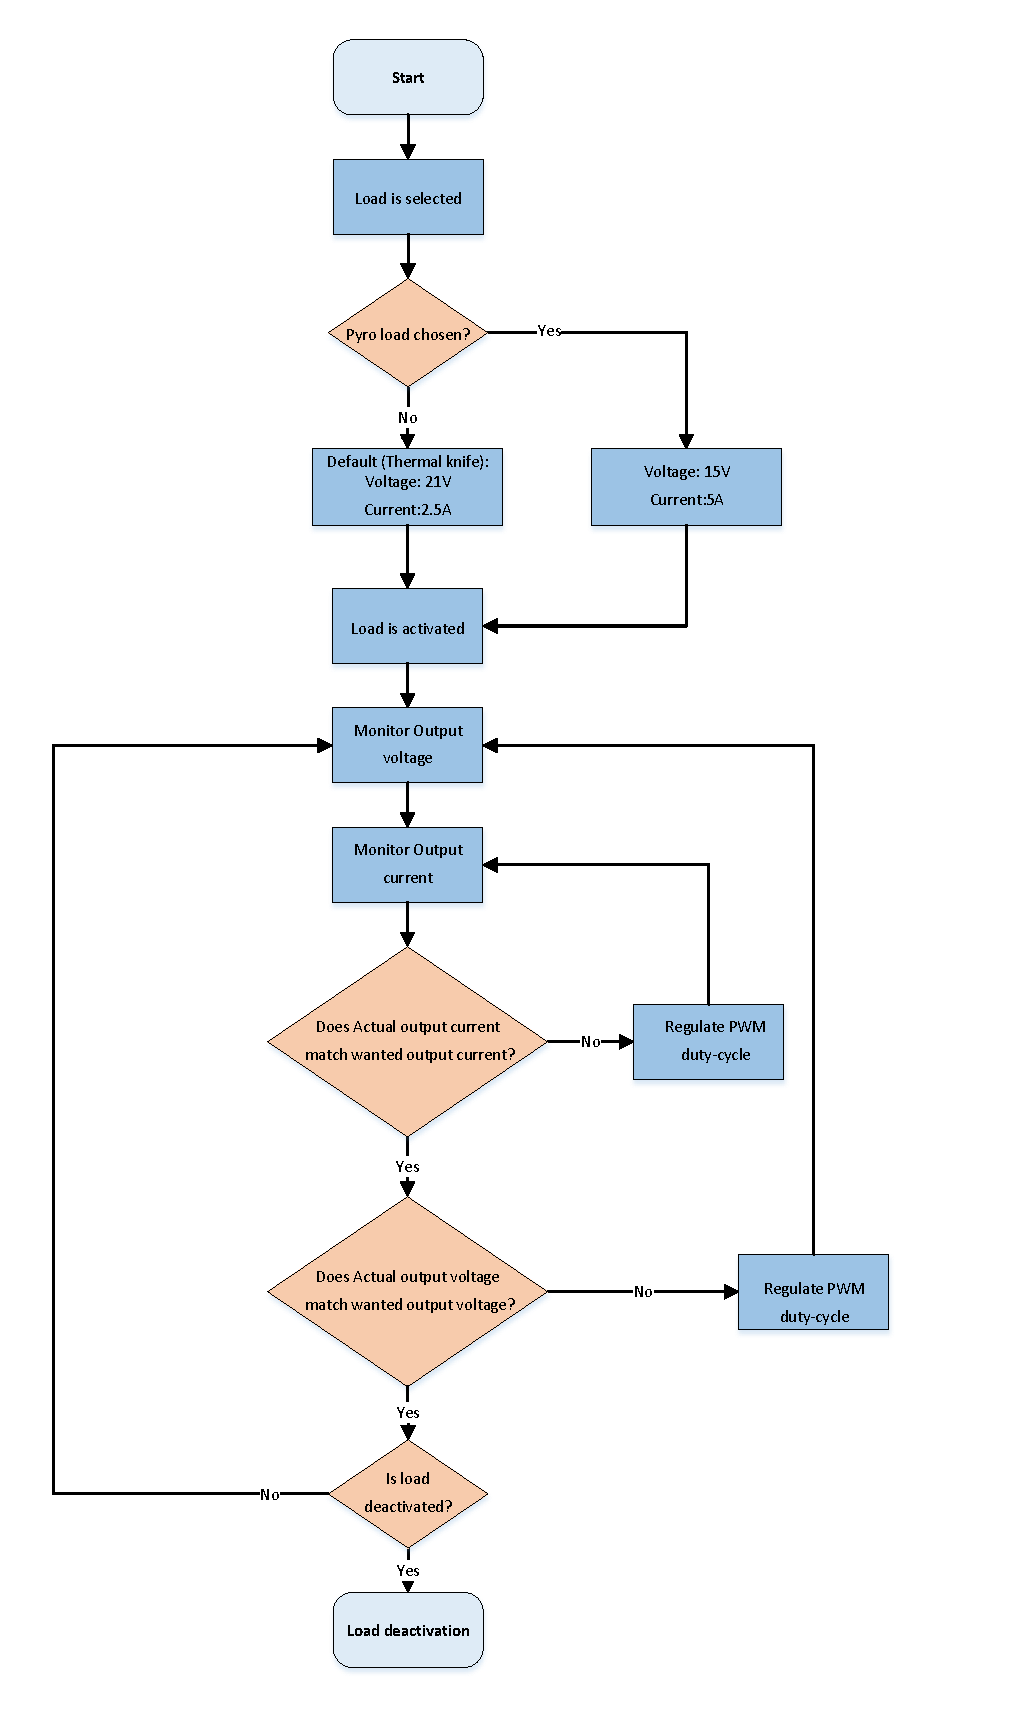
\includegraphics[width=0.7\linewidth]{../Dokumentation/tex/kravspecifikation/billeder/Flow_diagram.pdf}
	\caption{Flowdiagram for Universal Actuator Drive}
	\label{fig:flowdiagram}
\end{figure}
	
	
\chapter{Projektafgrænsning}
I dette afsnit er der beskrevet en afgrænsning af projektets indhold. Her er der taget udgangspunkt i det den ønskede funktionalitet af produktet, som sammenholdes med den egentlige opnåede funktionalitet. Elementer af projektet der er specificeret, men ikke implementeret er angivet i dette afsnit og uddybet i afsnit~\ref{future}. 

Produktets kernefunktionaliteter er prioriteret under udviklingen. Her er især prioriteret efter elementer, som kræves funktionsdygtige, før andre elementer kan udvikles. Her er udviklet en base for produktet, hvorpå flere krav og funktionaliteter skal kunne påføres.

Der blev valgt, at tage udgangspunkt i en converter med en statisk udgang. Dette ville skabe et udgangspunkt, og genere en erfaring, der ville give base for en videreudvikling til en dynamisk udgang af converteren.  

Det er valgt, at vikling af transformatoren sker af gruppen selv. Dette vil give en erfaring inden for området, der giver indsigt i hvad der er realistisk at designe efter. Derudover vil det også give et indblik i problematikkerne i vikling af en transformator. 

Converteren er designet efter de termiske krav, ved løbende vurdering og optimering af effekttabet i komponenterne.

Ved udvikling af elektroniske produkter til rumfart, kræves det udviklet med EEE-komponenter. Disse er meget omkostningsfulde, og er derfor ikke blevet brugt i projektet. Til gengælde er der brugt Terma-godkendte komponenter. Med disse komponenter har Terma en erfaring med, at opsætte disse til EEE-komponenter.  

Det blev specificeret at converteren skulle kunne operere ved et specifikt temperaturinterval. Det blev sikret ved kontrol af komponenternes specifikationer.

For at sikre en stabil indgangsspænding på converteren er det nødvendigt at implementere et indgangsfilter. Dette filter er blevet stillet tilrådighed af Terma, da det blev besluttet at fokusere andetsteds. Dette filter vil ikke blive beskrevet i denne rapport, men funktionaliteten af det er beskrevet i dokumentationen.

\fxnote{Beskriv PWM-forsyning}




	
	\chapter{Metode og proces}

\section{Metoder}

\subsection{ASE-modellen}
Til dette projekt er der brugt en iterativ udviklingsproces. Det er gjort da en iterativ proces er særligt velegnet til projekter, hvor kendskabet til domænet kan være begrænset. 

Der er taget udgangspunkt i den generelle ASE udviklingsmodel~\cite{udviklingsproces}, med den iterative proces trukket indover, hvilket ses på figur~\ref{fig:ASE}.
\begin{figure}[H]
	\center
	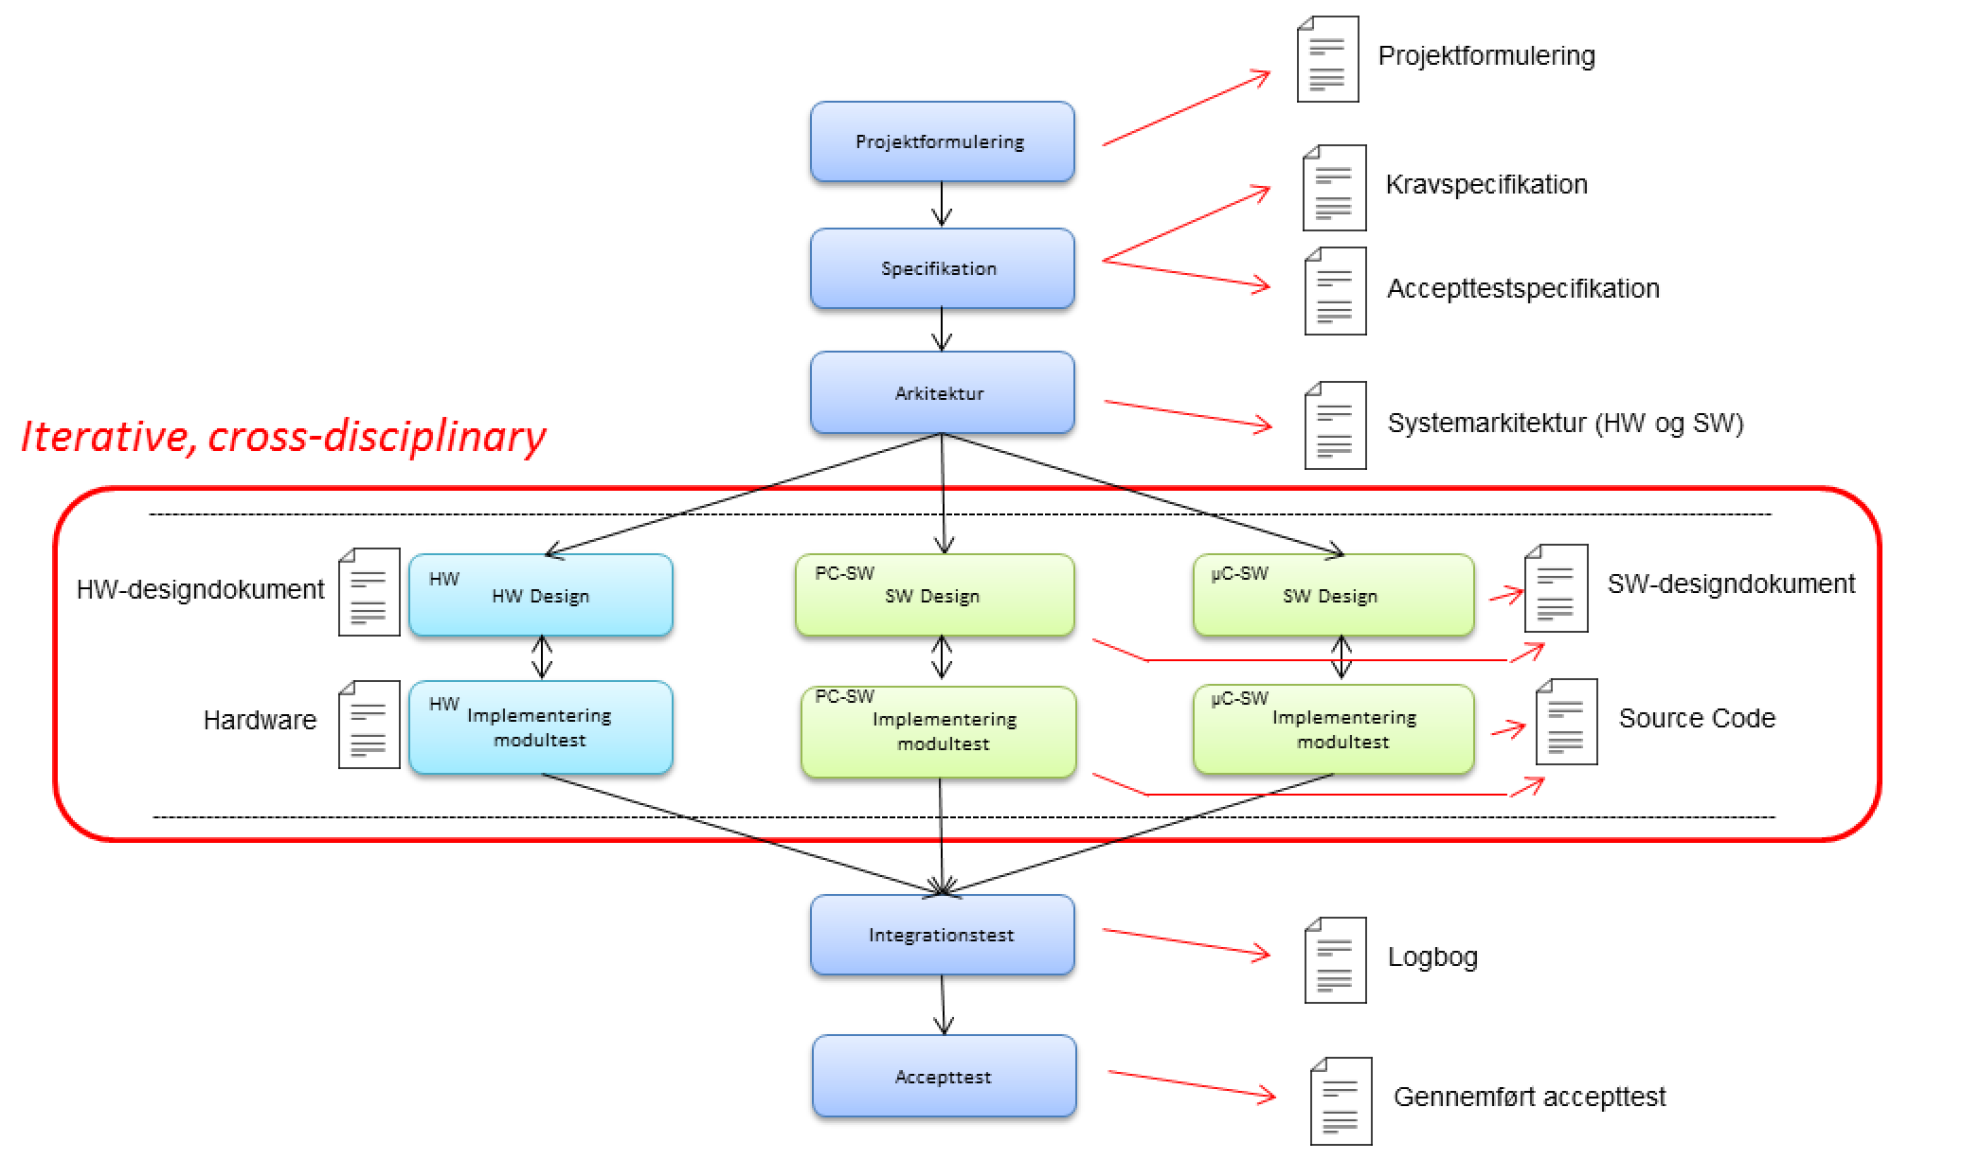
\includegraphics[max width=0.7\linewidth]{/tex/Metodeproces/billeder/ASEmodel.png}
	\caption{ASE model med fokus på iterativ proces}
	\label{fig:ASE}
\end{figure}  
I begyndelsen hvor produktet bliver specificeret med krav, har det ikke været så iterativt som de efterfølgende faser. Det skyldes at oplægget er kommet fra Terma, som har været med til at specificere kravene, og de har derfor ligget forholdsvis fast. Der har været få ændringer løbende, men det er begrænset.

Til gengæld har især design-, implementerings- og testfasen fungeret iterativt. Her er produktet blevet forbedret i små bider. Inden hver iteration begyndes gøres det klart, hvad der skal ske og hvad der skal opfyldes, inden næste iteration kan påbegyndes. 

\subsection{SysML}
Til at udarbejde systemarkitektur og design af systemet er der benyttet SysML. De anvendte SysML metoder for projektet har været block definitions diagrammer (BDD) og interne blok diagrammer (IBD). BDD'et er brugt til at nedbryde systemerne i mindre blokke, som dermed skal give et bedre overblik over systemets dele, og funktionen af disse. IBD'et viser den hardwaremæssige sammenhæng blokkene imellem.    

Ved at bruge er det nemmere for andre udviklere at sætte sig ind i systemet, og samtidig gør det designfasen nemmere, når systemets virkemåde er fastlagt forinden.

\subsection{UML}
Ofte benyttes UML mest til analyse og udarbejdelse af softwarearkitekturen. I dette projekt er UML metoden flowdiagram istedet brugt til at give et overblik over systemets ønskede virkemåde. Flow diagrammer giver et overblik over de valg, systemet gennemgår når det er aktivt.   

\subsection{MoSCoW} 
MoSCoW er en måde at prioritere krav på, alt efter hvor vigtige de er for det samlede produkt.  
De stilles op i "must", som er krav der skal overholdes. Næste prioritering er "should", som er krav der burde være overholdt. "Could" er features der ville være gode til produktet, men som der ikke forventes at være tid til at implementere. Sidste prioritering er "won't", hvilket er features som produktet ikke vil have. Med prioriteringen bør "must" kravene være opfyldt inden der kigges på "should" kravene. 

\section{Proces}
Som beskrevet tidligere har udviklingsprocessen fungeret iterativt. Til at implementere udviklingsmodellen, er der brugt Scrum~\cite{Scrum}. Scrum er valgt, da det er et projektsstyringsværktøj, begge medlemmer har haft stor succes med at bruge i tidligere semesterprojekter. Med en gruppe på to, er det ikke alle dele fra Scrum, som giver mening at bruge. Til dette projekt har det især været benyttet i forbindelse med daglige Scrum møder, og taskboards med backlog items. 

Til de daglige møder tages arbejdet fra dagen før op. Her forklares det, om man har været i stand til at udføre sine opgaver, og hvis ikke, hvilke problematikker det skyldes. Yderligere planlægges det, hvad der skal ske til næste gang. De daglige møder sørger for, at der bliver reflekteret over arbejdet løbende, hvilket sørger for at valgene der tages er gennemtænkt. 

Hver fase fra ASE modellen er blevet anset som iterationer, og har fået et taskboard hver. Hver enkelt iteration er delt op i mindre opgaver, der er lagt ind som backlog items på deres respektive taskboards. Design, implementerings og test iterationen er yderligere delt op i 3 faser for at bevare overblikket. På figur~\ref{fig:Taskboard} ses et øjebliksbillede af taskboardet for 3. iteration af design, implementerings og test.
\begin{figure}[H]
	\center
	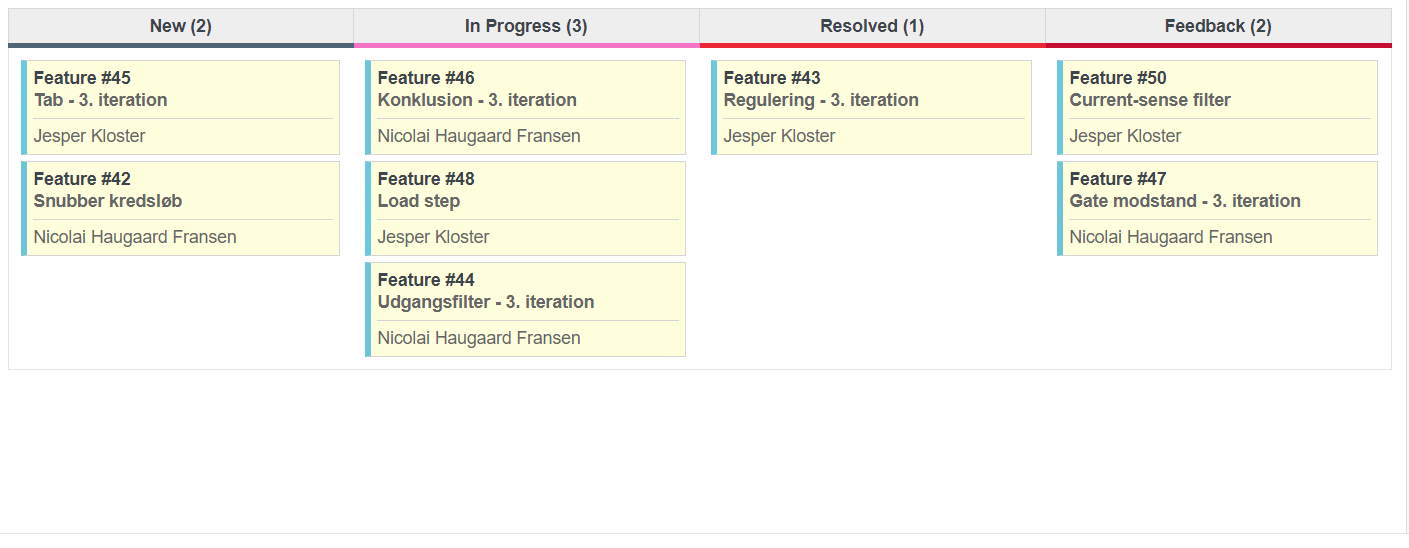
\includegraphics[max width=1\linewidth]{/tex/Metodeproces/Billeder/Scrumtask.png}
	\caption{Scrum taskboard}
	\label{fig:Taskboard}
\end{figure}        
Taskboardet sørger for at give et overblik over hvilke opgaver, der er påbegyndt og hvilke der mangles at blive lavet. På denne måde sikres det, at der ikke sidder to med samme opgave, og der er ikke opgaver, som bliver forsømt.

Til konfigurationsstyring er der benyttet et repository over Github~\cite{Github}. Det er brugt til deling af dokumenter og versionshistorik af disse. Yderligere er rapport, dokumentation og procesbeskrivelse skrevet i programmet LaTeX~\cite{Latex}. Kombinationen mellem LaTeX og Github gør det nemt at merge ændringer i dokumenterne. Det giver mulighed for at ændre i dokumenterne samtidigt, uden det skaber problemer. Samtlige dokumenter og bilag, som er vedlagt, har være administreret over Github.
Den interne kommunikation i gruppen er foregået over facebook. Det omhandler mødetidspunkter, spørgsmål og generelle informationer. Den eksterne kommunikation med vejleder og kontaktpersoner fra Terma er foregået over mail.  

Der har i projektperioden været afholdt 3 forskellige slags møder. De interne daglige møder, vejledermøde med Arne Justesen og eksterne møder med kontaktpersonerne fra Terma, Johnny Laursen og Hans Jensen. 

Langt hen ad vejen har der været afholdt vejledermøder en gang i ugen. Her har der på forhånd været tilsendt en dagsorden til vejlederen. Til møderne har der været en referent og en mødeleder, der sikrer, at dagsordenen overholdes. Disse roller er gået på skift fra møde til møde. Møderne har været brugt til, at diskutere arbejdet fra den forgangne uge og eventuelle opståede problemer. Derudover en forventning om opgaver der skal udføres inden næste møde. De omdiskuterede problemer har både været faglige- og rapportmæssige. 

Der har været afholdt møder med kontaktpersonerne fra Terma næsten hver uge. Igen har der været sendt information til kontaktpersonerne forinden, for at give et overblik om hvad der skal diskuteres. Ved disse møder har der været god mulighed for, at diskutere de fagligt opståede udfordringer, er opstået undervejs. Det er også her eventuelle ændringer af krav til produktet har været diskuteret. Under design-, implementerings- og testfasen har der dagligt været faglige diskussioner. Det har været yderst produktivt, at kunne løse et eventuelt problem med det samme, istedet for at vente til næste ugentlige møde. 

For yderligere information om den procesmæssige del af projektet henvises til dokumentet "Procesbeskrivelse" i bilagsmappen.  
	
	
\chapter{Analyse}
I dette afsnit beskrives de betragtninger og valg, der er blevet foretaget i løbet af produktudviklingen. Der er blevet vurderet på hvilke elementer der er nødvendige for realisering af produktet. Ved hvert af disse elementer er der foretaget en vurdering af hvilke muligheder og alternativer elementerne har. Der er også foretaget et vurdering på fordele og ulemper samtlige alternativer, der er blevet undersøgt i projektet. Ud fra disse vurderinger er der valget af de brugte teknologier blevet foretaget. 

\section{Converter topologi}
Converter topologien er en essentiel del af converterens endelige funktionalitet. Derfor er der undersøgt fordele og ulemper ved flere forskellige converter topologier. Converteren skal kunne konvertere indgangsspændingen til en mindre udgangsspænding, derfor er der udelukkende undersøgt topologier med denne funktionalitet. De undersøgte topologier er buck converteren, push-pull converteren og flyback converteren, som kan drives i både CCM og DCM. Disse convertere er yderligere beskrevet i dokumentationens afsnit 4.

\subsection{Buck converter}
Buck converteren er en af mere simple converter topologier, da den består af relativt få komponenter. sammen med dette er en af fordelene ved en buck converter, at der altid vil løbe en strøm i spolen. Det vil genere en minimal ripple-spænding på udganen, og derfor også et lille tab i udgangsfilteret. 

En stor ulempe ved buck converteren er at switch-komponenten, ofte en MOSFET, er placeret i den positive forsyningslinje. Det giver komplikationer ift. at drive MOSFET'en. Det vil kræve flere komponenter, og derfor også et mere kompliceret kredsløb. Af denne grund er buck converteren blevet fravalgt\cite{buck-converter}.

\subsection{Push-pull converter}

\subsection{Flyback converter}
Flyback converteren er en videreudvikling af buck converteren. Det er en transformator baseret topologi, som derfor giver et ekstra mulighed for effektoverførsel. Transformatoren erstatter spolen i buck converteren og derfor består de af det samme antal komponenter. Transformatoren giver desuden muligheden for sikre galvanisk adskillelse mellem indgangen og udgangen. 

En ulempe ved flyback converteren er en diskontinuert strømform i transformatoren, da der ikke løber strøm primær- og sekundærviklingen på samme tid. Det vil skabe større ripple- og RMS-strømme, og derved også genere et større tab i komponenterne\cite{SMPS-topologies}. 

En flyback converter kan drives på to overordnede måder - CCM og DCM. De to metoder bidrager yderligere med hver deres fordele og ulemper, som også vil blive beskrevet. 

Forskellen på de to metoder ligger i kurveformen for den strøm der løber i transformatorviklingerne. Ved CCM vil der altid løbe en strøm i enten den ene, eller den anden vikling. I modsætning til DCM hvor strømmen vil have en dødtid i løbet af en switch-periode. For at DCM skal kunne opretholde den samme udgangsstrøm som CCM, vil det betyde at peak- og RMS-strømmene ved DCM bliver større. Det giver derved anledning til et større effekttab. 

Fordelen ved at operere i DCM er primært en simplificering af reguleringssløjfen. CCM indeholder et dominerende nulpunkt langt nede i frekvens, der kan gøre systemet ustabilt, hvis der ikke tages højde for dette. Nulpunktet begrænser samtidig båndbredden, og dermed også systemets responstid. 

Ud fra disse undersøgelser er det blevet valgt, at arbejde videre med en flyback converter opereret i CCM. Dette vil sikre en converter hvor det er muligt, at holde effekttabet og kompleksiteten i converteren på et acceptabelt niveau. 

\section{Reguleringsmetode}
Der er to overordnede reguleringsmetoder der bruges til regulering i en DC/DC converter - Spændingsregulering og strømregulering. Ved spændingsregulering vil reguleringen udelukkende ske på baggrund af et spændingsfeedback til reguleringssløjfen. Ved strømregulering, reguleres der både efter strømmen og spændingen på udgangen. Det sikre en overstrømsbeskyttelse for converteren. Den ekstra reguleringsløkke vil samtidig simplificere reguleringen af en flyback converter i CCM. 

\noindent Derfor vælges det, at implementere en strømregulering i converteren. 

\section{PWM-controller}
PWM-controlleren er en central del af en DC/DC converter. Det er denne controller der står for at generere switch-signalet til converterens switch-element. Af denne grund er der mange krav PWM-controlleren skal leve op til. Den skal først og fremmest understøtte den valgt reguleringsmetode. Den skal kunne generere den maksimale duty-cycle der vil kunne fremstå i converterens switch-signal. Den skal kunne opretholde den valgte switch-frekvens. Derudover skal den også kunne generere et switch-signal med en amplitude der er høj nok, til at kunne drive den valgte MOSFET.

Ud fra disse krav, er det valgt at bruge en PWM-controller af typen UCC1801\cite{UCC1801}. Denne controller lever op til de førnævnte krav, og desuden understøtter den peak-current regulering. Den har indbyggede reguleringssløjfer, således nødvendigheden for eksterne komponenter mindskes. Derudover indeholder den flere sikkerhedsfunktioner ved opstart. Det er også en controller Terma har erfaringer med, og ved den kan omsættes til en lignende komponent der er godkendt til rumfart. 

\section{Transformator} \label{Transana}
Størrelsen på transformatoren betyder meget ift. temperaturstigningen, som en konsekvens af effektafsættelsen i transformatoren. Den termiske modstand i den er afhængig af størrelsen\cite{epcos-cores}. Derfor er det valgt at bruge en RM8\cite{RM8} som er den største kerne, der stadig overholder kravene for dimensionerne. Desuden er kernetypen RM blevet anbefalet af Terma, der har haft god erfaring med brug af disse i lignende konfigurationer. Der er valgt at bruge kernematerialet 3f3\cite{3f3}, da Terma har mere præcise målinger af materialets specifikationer, ift. databladets tolerancer.


	
	
\chapter{Systemarkitektur}
I det følgende afsnit beskrives systemarkitekturen, der er blevet udarbejdet i løbet af projektet. Projektet indeholder udelukkende hardware, derfor er der kun blevet udarbejdet arkitektur for dette. Arkitekturen ligger til grundlag for designprocessen i det videre projektforløb. Systemarkitekturen er overordnet beskrevet i det følgende afsnit, og uddybet i dokumentationens afsnit 3.

Hardwarearkitekturen er blevet beskrevet ved SysML's BDD og IBD. Der er blevet udarbejdet overordnede diagrammer for systemet, der skal give et overblik over det samlede system.

\section{Block Definition Diagram}
Figur~\ref{fig:BDD} viser et BDD for det samlede system. Det giver et overblik over de dele systemet indeholder, og hvilke forbindelser hver blok skal indeholde. 

\begin{figure}[H]
	\centering
	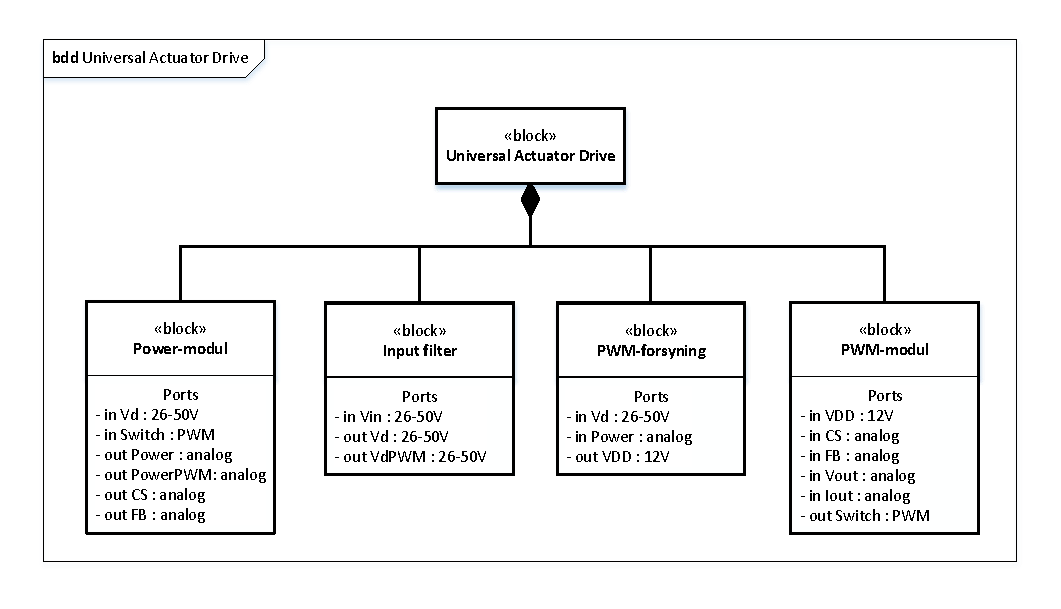
\includegraphics[width=1\linewidth]{../Dokumentation/tex/systemarkitektur/billeder/BDD.pdf}
	\caption{BDD for det overordnede system}
	\label{fig:BDD}
\end{figure}

\noindent Universal Actuator Drive består af fire overordnede blokke - et Power-modul, et Input-filter, en PWM-forsyning og et PWM-modul. Power-modulet indebærer selve effektoverførelsen fra indgang til udgang. Det er i dette modul de dominerende effektafsættelser sker, og derfor også her det termiske design skal optimeres. 

Input-filteret indebærer det filter der sikre en stabil indgangsspænding til Power-modulet. Derudover skal det fjerne højfrekvent ripple-spændinger fra indgangssignalet. 

\noindent PWM-forsyningen indebærer en regulator til regulering af PWM-modulets forsyningsspænding. Her vil der udvikles en metode der forsyner regulatoren fra indgangskilden under opstart, og udgangen når denne er stabil.

PWM-modulet indebærer PWM-controlleren der skal regulere udgangen til den ønskede belastning. Dette sker ved tilpasning af switch-signalet, samt strøm- og spændingsregulering af udgangen.

\section{Internal Block Diagram}
Figur~\ref{fig:IBD} viser et IBD for det samlede system. Det er blevet udarbejdet ud fra systemets BDD. IBD'et giver et overblik forbindelserne internt i systemet. Det viser også hvilke forbindelser systemet modtager fra andre systemer, altså grænsefladerne til omverdenen. Kravene for disse forbindelser er nærmere beskrevet i dokumentationens afsnit 3.2.

\begin{figure}[H]
	\centering
	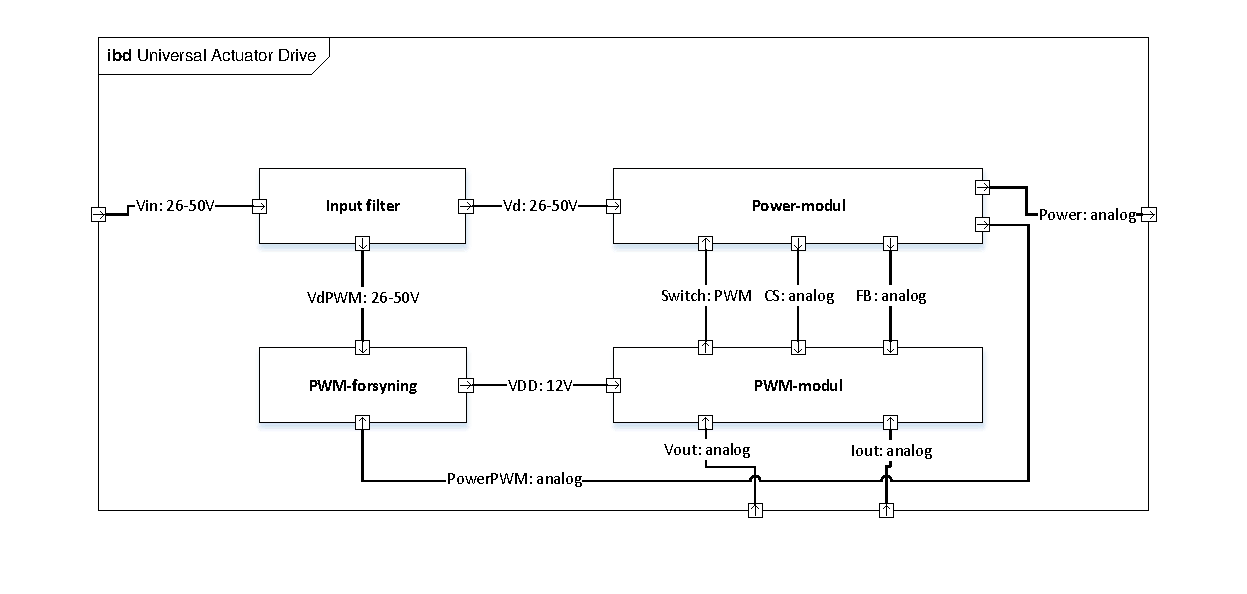
\includegraphics[width=1\linewidth]{../Dokumentation/tex/systemarkitektur/billeder/IBD.pdf}
	\caption{IBD for det overordnede system}
	\label{fig:IBD}
\end{figure}
	
	\chapter{Design, implementering og test}
I det følgende afsnit vil der blive gjort redde for designprocessen i projektforløbet. Her vil de meste essentielle dele for produktet blive beskrevet, mens en yderligere beskrivelse kan findes i dokumentationens afsnit 4-6.

Designprocessen blev delt op i tre overordnede iteration. I det følgende afsnit vil det derfor tydeliggøres, hvad der blev designet i den gældende iteration. 


\section{Første iteration}
Målet med 1. iteration var undersøgelse og valg af converter topologi. Herefter blev der opstillet en ideel simuleringsmodel for converteren, således analyse og simulering kunne sammenholdes. 
Kravet for at gå videre til 2. iteration, var opnåelse af en simulering der stemte overens med teorien. 



\subsection{Flyback converter - CCM}
Der blev valgt en flyback converter opereret i CCM, som converter topologi i projektet. En sådan converter deles op i en primær- og en sekundær side. Primærsiden består af transformatorens primærvikling og et switch-element, der typisk er en MOSFET. Sekundærsiden består af transformatorens sekundærvikling en diode, en kondensator og udgangsbelastningen. En oversigt over den ideelle flyback converter er vist på figur~\ref{fig:flyabck_ideal}. 

\begin{figure}[H]
	\centering
	\includegraphics[width=0.7\linewidth]{../Dokumentation/tex/1iteration/billeder/flyback_ideal.png}
	\caption{Ideelt diagram for flyback converteren
		\cite{SMPS-topologies}}
	\label{fig:flyabck_ideal}
\end{figure}

Når MOSFET'en er ON, vil der være en positiv spænding over primærviklingen ved prikenden af viklingen, der er lig indgangsspændingen. Da denne spænding er positiv, vil det få strømmen i viklingen til at stige lineært over den tid MOSFET'en er ON. Strømændringen er bestemt ud fra formlen:
\begin{equation}
V = L \cdot \frac{di}{dt}
\end{equation}

Fordi polariteten af sekundærviklingen er modsat primærviklingen, vil dioden være forspændt i spærreretningen da kondensatoren vil opretholde udgangsspændingen over belastningen. Når dioden ikke kan lede strømmen fra sekundærviklingen, vil transformatoren oplagre energi i kernen når MOSFET'en er ON. Når MOSFET'en går OFF vil strømmen i viklingen ikke kunne skifte momentant. Det vil vende polariteten af transformatoren, så der nu er en positiv spænding diode enden af sekundærviklingen. Nu vil dioden være forspændt i lederetningen, og derfor lede den energi der er blevet oplagret i kernen, i form af en strøm. Den strøm vil nu holde den ønskede udgang, men også oplade kondensatoren, således den kan opretholde udgangsspændingen i næste ON-periode. Da der nu vil være en negativ spænding over sekundærviklingen ift. prikenden af den, vil strømmen i viklingen aftage i løbet af MOSFET'ens OFF periode på baggrund af den førnævnte formel. 

Kurveformen for strømmene i en flyback transformator er vist på figur~\ref{fig:flyabck_ideal_currents}. Her ses det der blev forklaret før. Når MOSFET'en er ON, vil strømmen i primærviklingen rampe op, mens strømmen i sekundærviklingen er 0. Når MOSFET'en er OFF vil strømmen i sekundærviklingen rampe ned fra det niveau primærstrømmen nåede, mens strømmen i primærviklingen nu vil være 0. Niveau-forholdet mellem strømmene i viklingerne, vil blive bestemt af viklingsforholdet i transformatoren. Skal converteren bruges til omsætning af store spændingsændringer fra indgang til udgang, kan dette bruges for at mindske tabet. 

\begin{figure}[H]
	\centering
	\includegraphics[width=0.7\linewidth]{../Dokumentation/tex/1iteration/billeder/CCM_transformer_current.png}
	\caption{CCM transformator strømme}
	\label{fig:flyabck_ideal_currents}
\end{figure}

selvom transformatoren i helhed opererer i CCM, vil strømmene i individuelt i viklingerne være diskontinuerte. Det betyder peak-strømmene i viklingerne bliver større for at kunne opretholde den ønskede udgangsstrøm. 

\noindent Overføringsfunktionen for flyback converteren i CCM er\cite{SMPS-topologies2}:
\begin{equation*}
	V_{out} = \frac{N_s}{N_p} \cdot \frac{D}{1-D} \cdot V_{in}
\end{equation*}

Da den mindste indgangsspænding og største udgangsspænding converteren skal designes efter næsten er ens, vælges det at tage udgangspunkt i en transformator en et viklingsforhold på 1. Ud fra dette, og intervallet på indgangsspændingen på $26-50V$, kan den maksimale duty-cycle regnes til $D_{maks} = 0.447$ eller $44.7\percent$, og den minimale duty-cycle renes til $0.296$ eller $29.6\percent$.  

Selvinduktionen i transformatorviklingerne bestemmes ud fra den ønskede ripple-strøm i transformatoren og den valgte switch-frekvens. Der er valgt at tage udgangspunkt i en switch-frekvens på $100k\hertz$. Når der er valgt at have et omsætningsforhold på 1, vil denne selvinduktion være gældende for begge viklinger. Selvinduktionen i transformatoren kan designes ud fra følgende formel\cite{flyback-formler}:
\begin{equation*}
	L = \frac{V_{inmin} \cdot D_{min}}{I_{ripple} \cdot f_s}
\end{equation*}

RMS-strømmene i viklingerne har stor betydning for det endelige tab i converteren. Derfor estimeres de i den indledende fase, for at vurdere betydningen af dette. RMS-strømmen i primærviklingen regnes til $3.02A$, og RMS-strømmen i sekundærviklingen regnes til $3.36A$. Begge er regnet ved en indgangsspænding på $26V$. 

Den ideelle converter er simuleret, for kontrol af dens funktionalitet. Figur~\ref{fig:flyabck_ideal_diagram} viser diagrammet for den ideelle converter. Her er der udelukkende fokuseret på transformatoren. Desuden er der indsat en kondensator på $223\micro F$, for at mindske ripple-spændingen på udgangen. Udgangen er blevet simuleret til det forventede $21V$ og $2.5A$, mens RMS-strømmene i transformatorviklingerne stemte overens med det beregnede. 

\begin{figure}[H]
	\centering
	\includegraphics[width=0.7\linewidth]{../Dokumentation/tex/1iteration/billeder/flyback_ideal_diagram.png}
	\caption{Simulering af ideel flyback converter}
	\label{fig:flyabck_ideal_diagram}
\end{figure}

\noindent De præcise beregninger og simuleringer er beskrevet i dokumentationens afsnit 4.4.










\section{Anden iteration}
Målet for 2. iteration var, at indsætte ikke-ideele komponenter ind i modellen fra første iteration. Herudover skulle modellen implementeres for første gang. 
Kravet for at gå videre til 3. iteration var en funktionsdygtig implementeret converter. 
I dette afsnit beskrives hvordan nøglekomponenterne i konverteren er designet, og første implementering af converteren.

\subsection{Transformator}
Flyback converteren fungerer transformatoren lidt anderledes, i forhold til mange andre konstruktioner. Normalt vil der løbe en strøm i både den primære og sekundære vikling på samme tid. På den måde kan energien i transformatoren transformeres direkte fra den primære vikling til den sekundære vikling. Dette er ikke muligt i denne converter typologi, da der kun vil løbe strøm i én vikling ad gangen. Den energi, der skabes i den primære vikling, skal derfor kunne opbevares, indtil der begynder at løbe en strøm i sekundærviklingen. Sker det ikke, går kernen i mætning, hvilket vil sige, at der ikke er en lineær sammenhæng imellem transformatorens H-felt og B-felt.
Dette sikres ved, at indsætte et luftgab i kernen, som øger den magnetiske modstand. Det gør, at kernen kan opbevare mere energi.

I 1. iteration blev det valgt at tage udgangspunkt i en 1:1 transformator. Desuden er det i 2. iteration vigtigst, at få en velfungerende transformator. Derefter kan der senere optimeres på et mere optimalt viklingsforhold, hvis det vurderes nødvendigt. 

Med den estimerede nødvendige induktans beregnet i 1. iteration til $69.43\micro H$, blev energien, der induceres i primærviklingen udregnet til \begin{equation} \label{Primary_energy}
E = \frac{1} {2} \cdot L \cdot {I_{pk}}^2 = 1.083\milli J
\end{equation}

Denne energi skal kunne opbevares i kernen, for at undgå den føromtalte mætning. Hvornår en specifik transformator går i mætning afhænger af selve kernen og dets kernemateriale. Her faldt valget på en RM8 kerne og materialet 3f3, hvilket der er argumenteret for i sektion~\ref{Transana}.
På baggrund af databladet for 3f3, blev luftgabet designet efter at have et maksimalt B felt på $250mT$. Det gav et nødvendigt luftgap på:
\begin{equation} \label{Airgap}
l_g = \frac{L \cdot {I_{pk}}^2 \cdot \micro_0}{B^2 \cdot A_0} = 690.98\micro m
\end{equation}

Dette gav en fornyet induktans på $49\micro H$. Herefter bruges $A_L$ for 3f3 materialet og induktansen til at beregne vindingstallet, som blev udregnet og afrundet til 18 vindinger.
Analysen er herefter holdt op imod simuleringen i p-spice, at sikre at analyse og simulering stemmer overens.
 
Viklingen af transformatoren er sket med en kobbertråd med en diameter på $0.425mm$. Det er en tyndere tråd end analyseret, da der med den beregnede trådtykkelse på $0.45mm$ ikke i praksis kunne vikles 18 vindinger. Det har samtidig øget vindingstallet til 19, for stadig at udnytte hele kernens bredde bedst muligt. Med denne trådtykkelse og vindingstal er hele bredden af kernen på $8.6mm$ fuldt udnyttet. Igen for at fylde kernen ud, er der for både primær- og sekundærsiden viklet 3 viklinger i parallel, for at udnytte højden af kernen. Det giver samlet den tredobbelte højde med 6 viklinger i alt, hvilet ender i en højde $2.867mm$. Viklingen er udført ved skiftevis at vikle en primærvikling og en sekundærvikling. På den måde optimeres koblingen i transformatoren. Imellem viklingerne indsættes tape for at sikre det holdes stramt. På figur~\ref{fig: viklingsoverblik} vises et overblik over viklingerne og dimensionerne. 
\begin{figure}[H]
	\center
	\includegraphics[max width=0.7\linewidth]{../dokumentation/tex/2iteration/billeder/viklingsoverblik.png}
	\caption{Overblik over viklingsantal og tykkelse}
	\label{fig: viklingsoverblik}
\end{figure}
\noindent Med vindingstallet på 19 istedet for 18 er selvinduktionen og dermed strømmene i transformatoren igen korrigeret. Herunder ses den endelig analyserede selvinduktion, ripplestrøm og peakstrøm for den viklede transformator.
\begin{equation} \label{L_2}
L_2 = N^2 \cdot A_L = 57.76\micro H
\end{equation}
\begin{equation} \label{I_ripple_final}
I_{ripple} = \frac{V_{inmin} \cdot D_{max}}{L_2 \cdot f_s} = 2.01A
\end{equation}
\begin{equation} \label{I_pk_final}
I_{pk} = \frac{V_{out} \cdot I_{out}}{V_{inmin} \cdot D_{maks}} + \frac{I_{ripple}}{2} = 5.53A
\end{equation}
Den implementerede transformator ses på figur~\ref{fig: Viklettrans}
\begin{figure}[H]
	\center
	\includegraphics[max width=0.5\linewidth]{../dokumentation/tex/2iteration/billeder/Viklet_transformator.PNG}
	\caption{Viklet transformator}
	\label{fig: Viklettrans}
\end{figure}
\noindent Testen af transformatoren er udført ved at måle selvinduktionen i primær- og sekundærviklingerne samt spredningsselvinduktionen. Det er gjort med en impedansmåler. Her er der benyttet så korte ledninger som muligt samt 4-wire teknikken, for at undgå ekstra induktans fra ledningerne. 

For at måle selvinduktionen i primærviklingen måles henover primærviklingens to sider, mens sekundærviklingen holdes åben. Her laves et frekvenssweep fra $100Hz$ til $1MHz$. Samme fremgangsmåde for sekundærvikligen kan benyttes, men da transformatoren er 1:1, bør det være det samme.
Spredningsselvinduktionen er målt ved måle samme sted, henover primærviklingen, men derudover kortslutte sekundærviklingen. En ideel transformator vil give 0 i sådan en måling. Det betyder, at induktansen målt her, svarer til spredningsselvinduktionen. 

For yderligere forklaring af design, implementering og test af transformatoren henvises til dokumentationen afsnit 5.1, hvor dette er uddybet.

% Dokumentation af PWM-controller %
% UCC1801 %

\section{PWM-controller} \label{PWM}
PWM-controlleren er en vigtig del af en SMPS. Det er den der står for tilpasningen af switch-signalets duty-cycle, således udgangen holdes stabilt, når inputtet påvirkes eller ændres. Det er vigtigt at vælge PWM-controller ud fra kravene til converteren. PWM-controllere er ofte begrænset til en maksimal duty-cycle på enten $50\percent$ eller $100\percent$. Derudover skal der vælges, hvilken form for regulering af converterens udgangstrin der ønskes, da controlleren skal understøtte dette. 

Ud fra beregningerne af den maksimale duty-cycle i afsnit~\ref{maksimum_duty_cycle}, vælges det at PWM-controlleren maksimalt skal have en duty-cycle på $50\percent$. For at kunne opnå en mere præcis regulering, vælges det at bruge peak-current regulering. Denne form for regulering, regulerer efter peak-strømmen i transformatorens primærvikling. Da den regulere efter dette, opnås der også en strømbegrænser i regulerings-loopet. Ud fra disse krav vælges en PWM-controller af typen UCC1801\cite{UCC1801}. Det er en controller Terma har erfaring med, og derfor også nemt kan udskiftes med en space-godkendt controller.

\subsection{Funktionalitet}
På figur~\ref{fig:PWM_block_diagram} ses et funktionelt block diagram over UCC1801. Det indeholder controllerens overordnede komponenter, og giver et overblik over dens funktionalitet. 

\begin{figure}[H]
	\center
	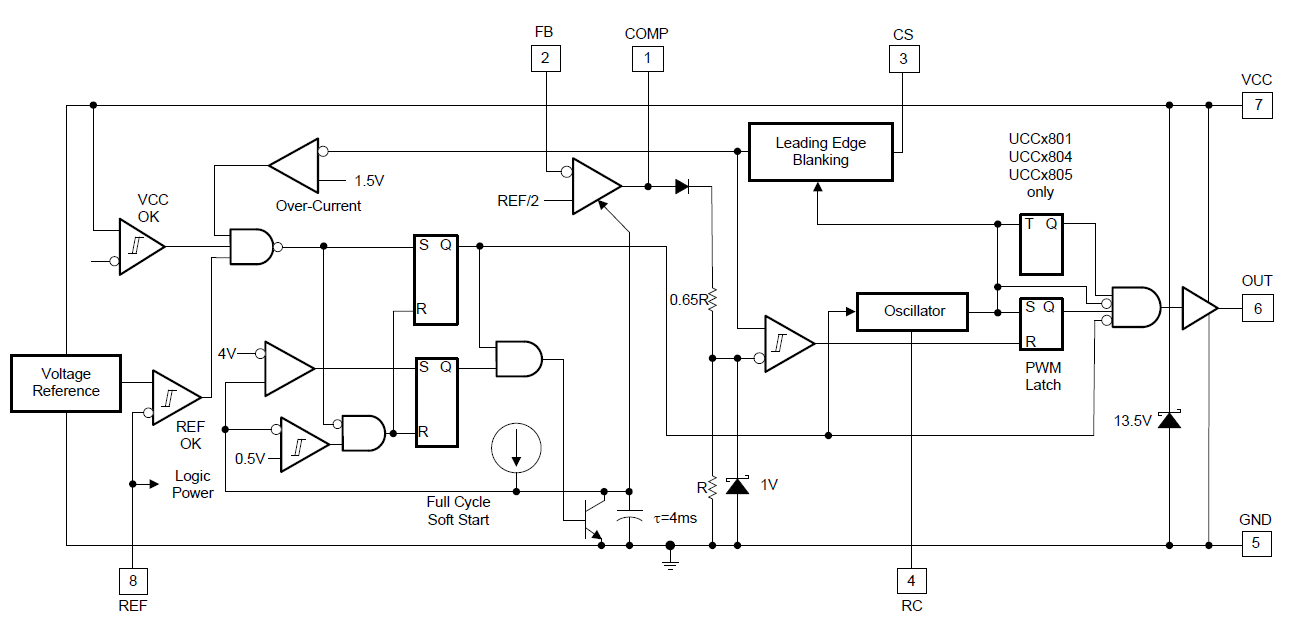
\includegraphics[max width=0.9\linewidth]{/tex/2iteration/billeder/PWM_block_diagram.PNG}
	\caption{UCC1801 - Funktionelt Block Diagram}
	\label{fig:PWM_block_diagram}
\end{figure}

Tabel~\ref{tab:ucc1801_specs} viser de mest essentielle specifikationer for UCC1801, i forhold til en flyback converter. Disse er udvalgte specifikationer fra databladet.

\begin{table}[H] 			
	\centering
	\begin{tabularx}{\textwidth}{|X|c|c|c|} 
		\hline
		\textbf{Specifikation} & \textbf{Min} & \textbf{Typ} & \textbf{Max} \\ \hline
		$V_{CC}$ &  &  & $12V$ \\ \hline
		$I_{out}$ &  &  & $1A$ \\ \hline
		$V_{Reference}$ & $4.925V$ & $5V$ & $5.075V$ \\ \hline
		$D_{max}$ & $48\percent$ & $49\percent$ & $50\percent$ \\ \hline
		$V_{on,th}$ & $8.6V$ & $9.4V$ & $10.2V$ \\ \hline
		$V_{off,th}$ & $6.8V$ & $7.4V$ & $8V$ \\ \hline
		Temperature Range & $-55\degreeCelsius$ &  & $125\degreeCelsius$ \\ \hline
		$f_{osc}$ & & & $1M\hertz$ \\ \hline
	\end{tabularx}

	\caption{Relevante specifikationer for UCC1801}
	\label{tab:ucc1801_specs}
\end{table}


\subsubsection{Ben konfiguration}
Der tages udgangspunkt i en UCC1801, med en PDIP pakke type. Figur~\ref{fig:ucc1801_pin_overview} viser en oversigt over ben konfigurationen for en sådan pakke. Det er en 8-bens IC, hvor samtlige ben bliver brugt. Benenes funktionalitet er overordnet beskrevet i tabel~\ref{tab:ucc1801_pin_functionality}, og vil blive uddybet i de følgende afsnit.

\begin{figure}[H]
	\center
	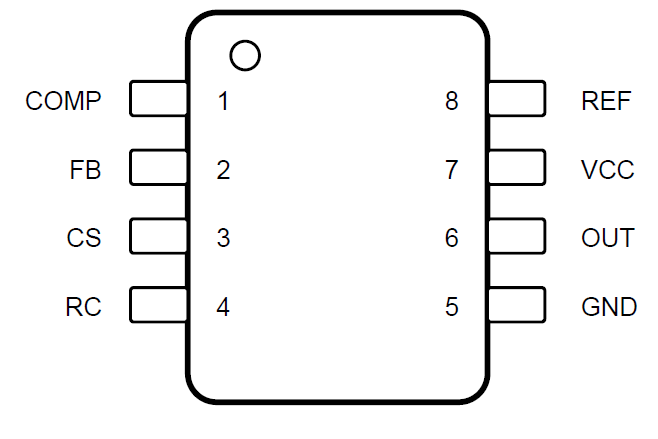
\includegraphics[max width=0.7\linewidth]{/tex/2iteration/billeder/ucc1801_pin_overview.PNG}
	\caption{Ben konfiguration for UCC1801}
	\label{fig:ucc1801_pin_overview}
\end{figure}

\begin{table}[H] 			
	\centering
	\begin{tabularx}{\textwidth}{|c|c|c|X|} 
		\hline
		\textbf{Navn} & \textbf{Ben} & \textbf{I/O} & \textbf{Beskrivelse} \\ \hline
		COMP & 1 & O & COMP er outputtet fra den indbyggede fejlforstærker. Dette ben bruges til at lave et feedback til FB benet i reguleringssløjfen. 	\\ \hline
		FB 	 & 2 & I & FB er inputtet til den indbyggede fejlforstærker. Den er forbundet til den inverterende indgang af forstærkeren. Den bruges sammen med COMP, som en del af reguleringssløjfen.\\ \hline
		CS   & 3 & I & CS er inputtet til current sense komparatorne. UCC1801 har to komparatorere til current sense: PWM komparatoren og overstrøms komparatoren. PWM-komparatoren bruges til, at trække udgangssignalet lavt, når CS-signalet overstiger $1V$. Overstrøms komparatoren er en indbygget overstrømsbeskyttelse. Den tvinger udgangen lav, så længe CS-signalet er over $1.5V$ \\ \hline
		RC 	 & 4 & I & RC er inputtet til oscillatoren. Oscillator frekvensen, og dermed også switch-frekvensen, sættes ud fra tidskonstanten mellem en modstand og en kondensator.  \\ \hline
		GND  & 5 & - & GND er ground for IC'ens komponenter.  \\ \hline
		OUT  & 6 & O & OUT er IC'ens output. Det er et PWM-signal, hvis duty-cycle afhænger af PWM-komparatoren. Outputtet skiftes mellem GND og VCC, hvilket betyder at VCC skal være høj nok, til at drive MOSFET'en.  \\ \hline
		VCC  & 7 & I & VCC er forsyning til IC'ens komponenter. Det foreslås at vælge en høj VCC, for at mindske støjpåvirkninger. For at mindske støj på forsyningen anbefales det, at bypasse VCC med en kondensator på minimum $1\micro \farad$, tæt på IC'en. \\ \hline
		REF  & 8 & O & REF er outputtet for IC'ens interne spændingsreference. Den bruges bl.a. som reference til fejlforstærkeren. Derudover forsyner den IC'ens logiske komponenter. For at mindske støj på referencen, anbefales det at bypasse REF med en kondensator på minimum $1\micro \farad$, tæt på IC'en. \\ \hline
	\end{tabularx}
	
	\caption{Ben funktionalitet for UCC1801}
	\label{tab:ucc1801_pin_functionality}
\end{table}

\subsection{Under Voltage LockOut}
UCC1801 indeholder en Under Voltage LockOut (UVLO) beskyttelse. Dette betyder at forsyningsspændingen skal være et bestemt niveau, før controlleren starter. Som en konsekvens af dette vil både outputtet og referencespændingen holdes lav, indtil grænseværdien er nået. For at have en hysteresemargin, har den både et turn ON og et turn OFF niveau. Ved UCC1801 er disse niveauer $V_{on,th}=9.4V$ og $V_{off,th}=7.4V$. Da amplituden af output-signalet er lig VCC, vil controlleren ikke prøve at drive MOSFET'en før $V_{CC}=9.4V$. Da en MOSFET typisk har en $V_{gs,th}$ mellem $4$ og $5V$, vil der ikke opnås et stadie hvor MOSFET'en kun er delvist ON. Dette ses også på referencespændingen, da den først bliver $5V$ når $V_{CC}\geqslant 9.4V$. Referencen kan derfor også bruges, som en ON/OFF indikator. 

\subsection{Switch-frekvens}
Controllerens switch-frekvens sættes af oscillator blokken i block diagrammet. Den genererer en savtand-spænding, som trigger den efterfølgende latch. Dette giver et PWM-signal, da det skifter mellem VCC og GND.
Stigetiden for savtand spændingen bliver bestemt af tidskonstanten for et eksternt RC-kredsløb. Faldetiden for signalet bliver bestemt af den eksterne kondensator, samt ON-modstanden i en intern transistor. Den on-modstand er opgivet til ca. $130\ohm$. Denne faldetid vil begrænse den maksimale duty-cycle, da outputtet vil være lavt i løbet af faldetiden. 

\begin{figure}[H]
	\center
	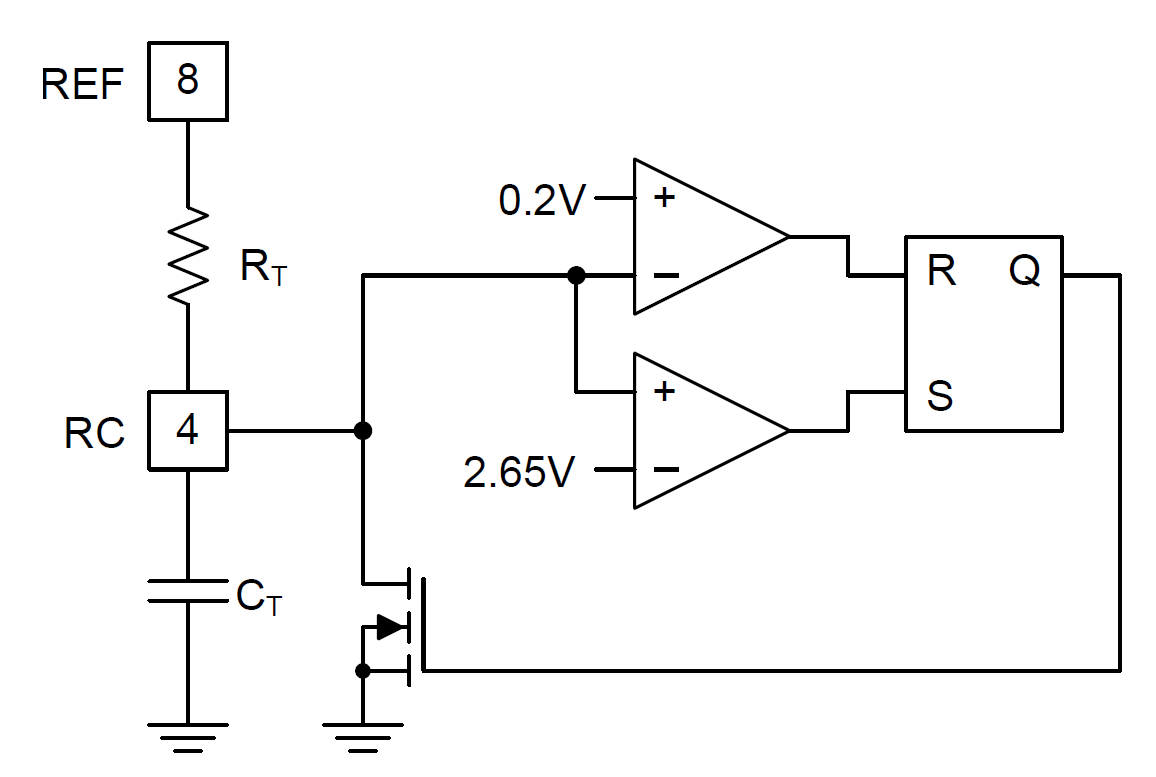
\includegraphics[max width=0.7\linewidth]{/tex/2iteration/billeder/PWM_oscillator_diagram.PNG}
	\caption{Oscillator diagram}
	\label{fig:PWM_oscillator_diagram}
\end{figure}

Figur~\ref{fig:PWM_oscillator_diagram} viser et ækvivalent diagram for oscillator blokken. Komponenterne $R_T$ og $C_T$ er det eksterne RC kredsløb, mens resten er interne komponenter. På diagrammet ses det at operationsforstærkerne er koblet til henholdsvis $0.2V$ og $2.65V$. Dette sætter maksimum og minimum for savtand spændingen. 

Da der skal komme en flanke på output-signalet hver gang savtand spændingen rammer maksimum, skal frekvensen af savtand spændingen være den dobbelte af den ønskede switch-frekvens. Der ønskes en switch-frekvens på $100k\hertz$, derfor sættes oscillator frekvensen til $f_{osc}=200k\hertz$. I databladet er det anbefalet at $R_T$ vælges mellem $10k\ohm$ og $200k\ohm$, mens det anbefales at $C_T$ vælges mellem $100p\farad$ og $1000p\farad$. Formel~\ref{f_osc} er opgivet i databladet og bruges til at estimere RC komponenterne. $C_T$ sættes til $200p\farad$, og $R_T$ beregnes:
\begin{equation} \label{f_osc}
R_{T} = \frac{1.5}{f_{osc} \cdot C_T} = \frac{1.5}{f_{osc} \cdot C_T} = 37.5k\ohm
\end{equation}
Ved et opslag i databladet ses det, at med en $C_T=200p\farad$ kan der maksimalt opnås en duty-cycle på ca. $48.9\percent$. Da converteren maksimalt skal opererer med en duty-cycle på $44.7\percent$, godtages dette.

\subsection{Current sense kredsløb} \label{CS_loop}
Som nævnt i afsnit~\ref{PWM} er der valgt at bruge peak-current regulering. Denne form for regulering består af to reguleringssløjfer - en spændings- og en strømsløjfe. I dette afsnit beskrives dimensioneringen af strøm sløjfen, mens spændingssløjfen beskrives i afsnit~\ref{V_loop}.

Current sense kredsløbet består, som minimum, af en current sense modstand. Denne modstand bruge til at konvertere strømmen i transformatorens primærvikling om til en spænding. Denne konvertering vil gøre, at kurveformen for strømmen og spændingen er ens, dog med en faktor til forskel. PWM-komparatoren i controlleren trigger udgangen, når current sense spændingen er rampet op til $1V$. Derfor skal modstanden dimensioneres således, spændingen over den er lig $1V$ når peak-strømmen i transformatoren er lig $5.53A$. Dette regnes ud fra Ohm's lov:
\begin{equation} \label{R_cs}
R_{cs} = \frac{1V}{5.53A} = 0.181\ohm
\end{equation}

Da den mindste modstandsværdi der er til rådighed er på $1\ohm$, vil der blive brugt $6\cdot 1\ohm$ i parallel. Dette vli give en modstandsværdi på $0.167\ohm$. 



\subsubsection{Filtrering}
På grund af switching-spikes i MOSFET'en, når den går ON, vil der også komme spikes på current sense signalet. Hvis disse spikes når et niveau der er højere end $1V$, vil det trigger komparatoren. Dette vil få controlleren til at generer et PWM-signal, der er meget lavere end det ønskede. Derfor implementeres der et filter, for at filtrere disse spikes væk.

UCC1801 har et indbygget digitalt filter, kaldet Leading Edge Blanking. Dette filter er designet til at filtrere de første $100ns$ af signalet væk, og dermed fjerne spiken. Ideelt set vil dette give et signal, som ses på figur~\ref{fig:ucc1801_leading_edge}.

\begin{figure}[H]
	\center
	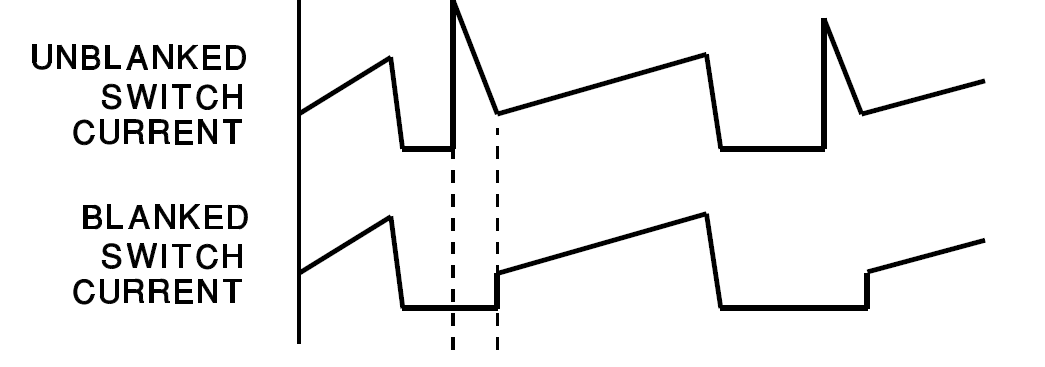
\includegraphics[max width=0.7\linewidth]{/tex/2iteration/billeder/ucc1801_leading_edge.PNG}
	\caption{Current sense signal før og efter Leading Edge Blanking}
	\label{fig:ucc1801_leading_edge}
\end{figure}

Det digitale filter er ikke altid tilstrækkeligt, og derfor designes et eksternt analogt RC-filter, for yderligere filtrering. Det designes til at have en stige tid på $300ns$, for at tilføje en yderligere filtrering på ca. $200ns$. 

\noindent Med en stige tid på $300ns$, kan båndbredden af filteret estimeres:
\begin{equation} \label{filter_BW}
BW \approx \frac{0.34}{t_r} \approx 1.133M\hertz
\end{equation}

\noindent Der vælges en kondensator på $C_f=100pF$. Ud fra kondensatoren og den ønskede båndbredde i filteret, regnes modstanden.
\begin{equation} \label{filter_R}
R_f = \frac{1}{2 \cdot \pi \cdot BW \cdot C_f} = 1.4k\ohm
\end{equation}

Med det designede filter vil stige tiden af current sense signalet, nu blive begrænset af filteret. Derfor vil den første de af signalet nu ligne et første ordens system, der stiger indtil spændingen når det niveau der svarer til strømmen i primærviklingen. Derefter vil signalet stige som en ret linje, ligesom strømmen. Dette ses på figur~\ref{fig:ucc1801_CS_filter}, hvor det øverste signal er før filteret, og det nederste er efter.

\begin{figure}[H]
	\center
	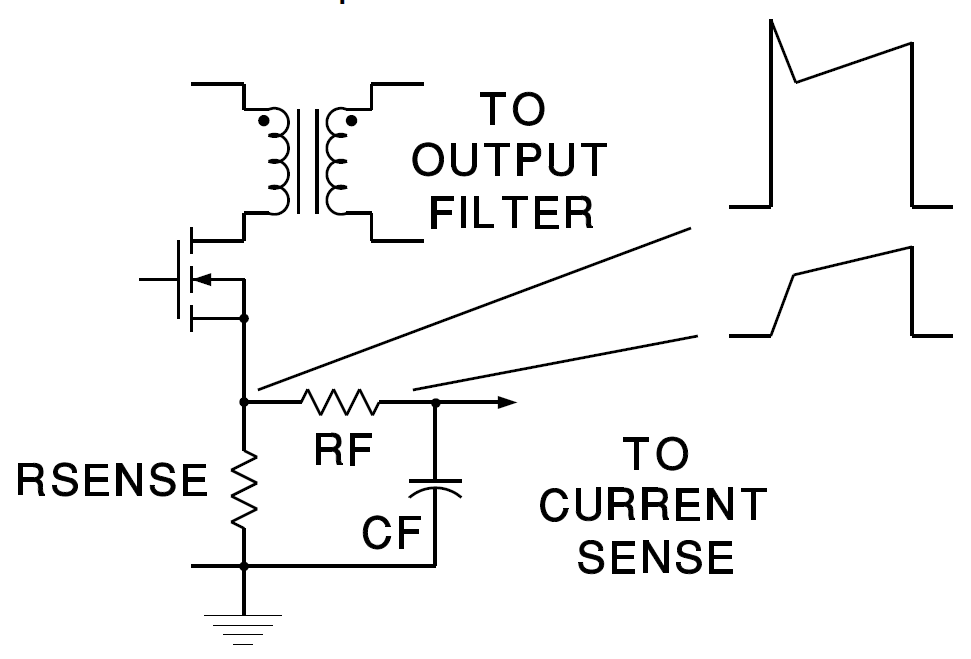
\includegraphics[max width=0.7\linewidth]{/tex/2iteration/billeder/ucc1801_CS_filter.PNG}
	\caption{Current sense signal før og efter eksternt RC-filter}
	\label{fig:ucc1801_CS_filter}
\end{figure}

\subsubsection{Overstrømsbeskyttelse} \label{CS_protection}
En fordel ved, at regulere efter strømmen i transformatoren er, at der opnås en overstrømsbeskyttelse. Når strømmen stiger, vil PWM-controlleren sænke duty-cyclen, og derved også sænke udgangsspændingen. Dette giver en I/V karakteristik der, ideelt set, er næsten firkantet. Dette er skitseret på figur~\ref{fig:I-V_karateristik}. 

\begin{figure}[H]
	\center
	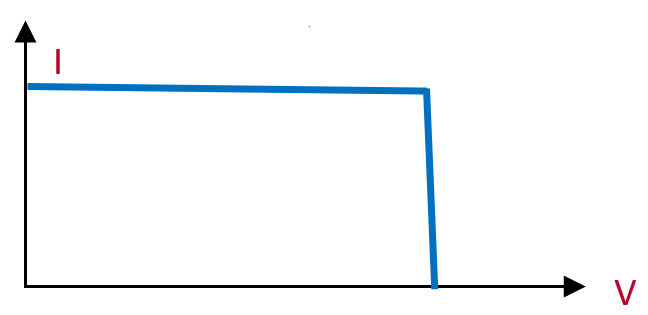
\includegraphics[max width=0.7\linewidth]{/tex/2iteration/billeder/I-V_karakteristik.PNG}
	\caption{I/V karakteristik for converteren}
	\label{fig:I-V_karateristik}
\end{figure}

Denne karakteristik kan dog ikke opnås i realiteten. Filteret der er indsat for at filtrere current sense signalet, vil lave en hale på karakteristikken. Det sker fordi controlleren ikke ser den faktiske strøm, men den filtrerede, når duty-cyclen er lav. 

Da det er nødvendigt at filtrere current sense signalet, men samtidig påvirker converterens I/V karakteristik, optimeres filteret ofte således, det kun akkurat filtrer nok. Denne optimering vil ske i 3. iteration. 

\subsection{Spændingsregulering} \label{V_loop}
I dette afsnit beskrives spændingssløjfen. Den består hovedsageligt af to dele: en spændingsdeler og en fejlforstærker. Spændingsdeleren deler udgangsspændingen ned, så den ønskede udgangsspænding er lig en intern reference i IC'en. Fejlforstærkeren står for selve reguleringen. Den inverterende indgang og udgangen på fejlforstærkeren er ført ud, således det er muligt at indsætte et kompenseringsnetværk.

\subsubsection{Spændingsdeler}
Den ikke inverterende indgang på den indbyggede fejlforstærker i UCC1801, er forbundet til den halve reference spænding, dvs. $2.5V$. Derfor skal der designes en spændingsdeler, der deler den ønskede udgangsspænding på $21V$ ned til $2.5V$. Figur~\ref{fig:Voltagedivider_ideal} viser kredsløbet for spændingsdeleren. 

\begin{figure}[H]
	\center
	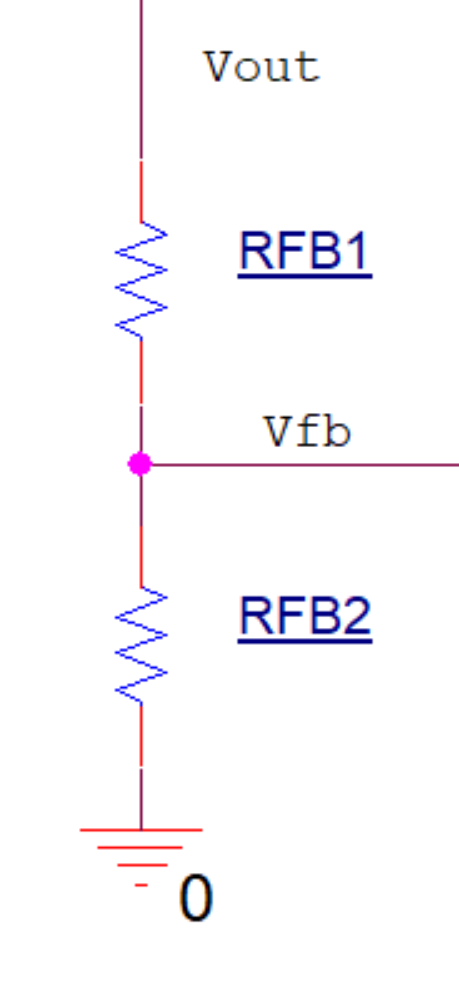
\includegraphics[max width=0.7\linewidth]{/tex/2iteration/billeder/Voltagedivider_ideal.PNG}
	\caption{Spændingsdeler diagram}
	\label{fig:Voltagedivider_ideal}
\end{figure}

Spændingsdeleren designes således der løber en strøm på $1mA$ i den. Derved påvirker den ikke udgangsstrømmen. Derudover dimensioneres de to modstande, således der er et spændingsfald på $2.5V$ over $R_{FB2}$, og $21V-2.5V$ over $R_{FB1}$. $R_{FB1}$ er beregnet med ligning~\ref{RFB1}.

\begin{equation} \label{RFB1}
R_{FB1} = \frac{V_{out}-V_{FB}}{I_{FB1}} = \frac{21V-2.5V}{1mA} = 18.5k\ohm
\end{equation}

\noindent $R_{FB2}$ er beregnet ud fra spændingsdeler formlen, ligning~\ref{RFB2}. Her løses $R_{FB2}$, og fås til $R_{FB2}=2.527k \ohm$.  
\begin{equation} \label{RFB2}
V_{FB} = \frac{R_{FB2}}{R_{FB1} + R_{RB2}} \cdot V_{out}
\end{equation}

For at opnå en præcis spændingsdeler vælges der at bruge to modstande i parallel. Den ene modstand vælges til $R_{FB21}=2.55k\ohm$. Mens den anden regnes ud fra den ønskede samlede modstandsværdi. Dette gøres ved ligning~\ref{RFB22}, som løses med hensyn til $R_{FB22}$. Dette giver $R_{FB22}=280.5k\ohm$, som afrundes til $280k\ohm$.
\begin{equation} \label{RFB22}
R_{FB2} = ((R_{FB21})^{-1} + (R_{FB22})^{-1})^{-1}
\end{equation}

\subsubsection{Fejlforstærker}
Som en del af reguleringen opstilles der først en overføringsfunktion for power-modulet. Denne overføringsfunktion er opgivet i databladet for UCC1801, og er skrevet ved ligning~\ref{H_Power}.
\begin{equation} \label{H_Power}
G_{pwr}(s) = G_0 \cdot \frac{(1+\frac{s}{2\pi \cdot f_{ESRz}}) \cdot (1-\frac{s}{2\pi \cdot f_{RHPz}})}{1+\frac{s}{2\pi \cdot f_{p1}}} \cdot \frac{1}{1 + \frac{s}{2\pi \cdot f_{p2}} + \frac{s^2}{(2\pi \cdot f_{p2})^2}}
\end{equation}

Overføringsfunktionen består af flere dele: en DC-forstærkning, to poler og to nulpunkter. DC-forstærkningen, $G_0$, er skrevet ved ligning~\ref{DC_gain}. Den er især bestemt af belastningen, current sense kredsløbet, transformatoren og switch-frekvensen. Den regnes til en forstærkning på $10.74$ gange, eller $20.6\decibel$.
\begin{equation} \label{DC_gain}
G_0 = \frac{R_{out} \cdot N}{R_{CS} \cdot A_{CS}} \cdot \frac{1}{\frac{(1-D)^2}{\tau_L} + (2 \cdot M) + 1} = 10.7GG \Rightarrow 20.6\decibel
\end{equation}
\noindent Hvor:
\newline \noindent $N$ er omsætningsforholdet i transformatoren.
\newline \noindent $A_{CS}$ er den interne forstærkning i current sense kredsløbet, og aflæses i databladet til $1.65$.
\newline \noindent $D$ er den maksimale duty-cycle, som er $0.447$.
\newline \noindent $\tau_L$ er converterens tidskonstant. Den regnes ud fra ligning~\ref{tau_L}.
\begin{equation} \label{tau_L}
\tau_L = \frac{2 \cdot L_P \cdot f_s}{R_{out} \cdot N^2}
\end{equation}
\newline \noindent $M$ er spændingsomsætningen fra indgang til udgang. Den regnes ud fra ligning~\ref{M}.
\begin{equation} \label{M}
M = \frac{V_{out} \cdot N}{V_{in}}
\end{equation}

En flyback converter, som opererer i CCM, har to primære nulpunkter der kan påvirke stabiliteten i systemet. Det er også de to nulpunkter der er inkluderet i overføringsfunktionen. Den ene, $f_{ESRz}$, er bestemt af produktet mellem udgangskapaciteten og den indre seriemodstand i udgangskondensatoren. Placeringen af denne er regnet ved ligning~\ref{ESR_zero}.
\begin{equation} \label{ESR_zero}
f_{ESRz} = \frac{1}{2 \cdot \pi \cdot R_{ESR} \cdot C_{out}} = 189.5k\hertz
\end{equation}

Det andet nulpunkt er højre-halvplans-nulpunktet. Det er ofte dette nulpunkt der er det dominerende af de to, og derfor den der skal tages højde for i reguleringen. Placeringen af dette er regnet ved ligning~\ref{RHP_zero}. Placeringen af dette nulpunkt, er afhængigt af størrelsen på belastningen, samt inputspændingen. Placeringen stiger ved højere inputspændinger, og mindre belastninger. 
\begin{equation} \label{RHP_zero}
f_{RHPz} = \frac{R_{out} \cdot (1-D)^2 \cdot N^2}{2 \cdot \pi \cdot L_P \cdot D} = 15.8k\hertz
\end{equation}

\noindent Ud fra ligning~\ref{ESR_zero} og \ref{RHP_zero}, ses det, at det er højre-halvplans nulpunktet der er det dominerende nulpunkt i converteren. Når båndbredden skal vælges, er det derfor vigtigt, at den ligger tilpas meget lavere end det dominerende nulpunkt.

Converteren har også to relevante poler. Den dominerende pol bestemmes af load'en og udgangskondensatoren. Den anden pol er placeret ved den halve switching-frekvens. De to poler er beregnet ved ligning~\ref{pol1} og \ref{pol2}.
\begin{equation} \label{pol1}
f_{p1} = \frac{\frac{(1-D)^3}{\tau_L} + 1 + D}{2\cdot \pi \cdot R_{out} \cdot C_{out}} = 132.8\hertz
\end{equation}

\begin{equation} \label{pol2}
f_{p2} = \frac{f_s}{2} = 50k\hertz
\end{equation}

\noindent Bode plottet for power-modulet plottes i MATLAB på figur~\ref{fig:MATLAB_power_module}. Her aflæses DC-forstærkningen til $20.6\decibel$. Derudover aflæses der en pol ved ca. $130\hertz$ og ved ca. $50k\hertz$. Dette stemmer overens med de beregnede værdier.

Konsekvensen af højre-halvplans nulpunktet ses også tydeligt på figur~\ref{fig:MATLAB_power_module}. Når frekvensen nærmer sig nulpunktet bliver forstærkningen øget med $20 \decibel$/decade, som ved et venstre-halvplans nulpunkt. Tilgengæld vil fasen blive trukket ned med $90^\circ$, i stedet for op. Da polen fra switch-frekvensen ligger ca. samme sted, og også trækker fasen ned med $90^\circ$, kommer der et stort fasedrej i dette frekvensområde. Det kan gøre systemet ustabilt hvis gain-marginen ikke er tilstrækkelig stor. 

\begin{figure}[H]
	\center
	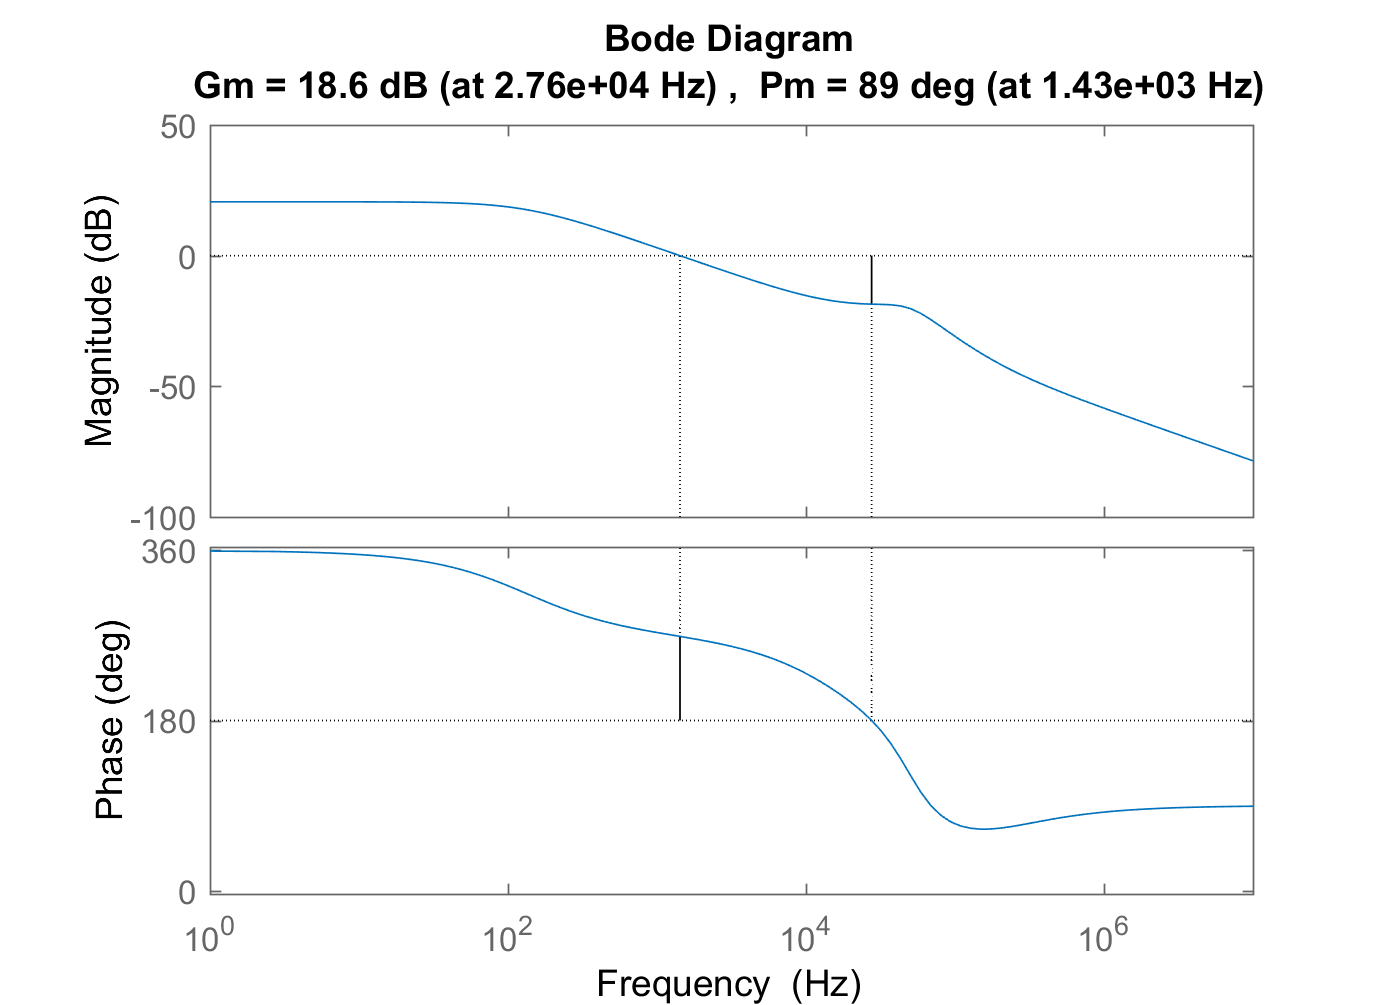
\includegraphics[max width=0.7\linewidth]{/tex/2iteration/billeder/MATLAB_power_module.PNG}
	\caption{Bode plot for power-modulet}
	\label{fig:MATLAB_power_module}
\end{figure}

I denne iteration designes der et kompensationsnetværk der vil sikre et stabilt system, med en lav båndbredde. Dette vil blive optimeret i en senere iteration. 
Da der ønskes en lavere båndbredde, end det converteren har i forvejen, indsættes et RC-led i serie som kompensationsnetværk. Ved at bruge et RC-led, vil kondensatoren bestemme forstærkningen ved lave frekvenser, fordi impedansen her er stor. Mens modstanden vil bestemme forstærkningen ved høje frekvenser, fordi kondensatoren vil blive set som en kortslutning. 

Den endelige båndbredde af systemet ønskes på ca. $800\hertz$. Det vil sikre, at systemet ikke bliver ustabilt. For at opnå den ønskede båndbredde aflæses det ud fra bode plottet på figur~\ref{fig:MATLAB_power_module}, at forstærkningen skal mindskes med ca. $5.4\decibel$, eller ca. $0.535GG$, ved frekvenser over $800\hertz$. Den samlede forstærkning af reguleringssløjfen, bestemmes af produktet mellem forstærkningen i spændingsdeleren og forstærkningen i fejlforstærkeren. Forstærkningen i spændingsdeleren regnes ved ligning~\ref{voltagedivider_gain}.
\begin{equation} \label{voltagedivider_gain}
g_{FB} = \frac{R_{FB2}}{R_{FB1}+R_{FB2}} = 0.12
\end{equation}

\noindent Nu kan feedback modstanden i fejlforstærkeren regnes ved ligning~\ref{error_opamp_gain}. 
\begin{equation} \label{error_opamp_gain}
g_{tot} = \frac{R_{comp}}{R_{par}} \cdot g_{FB}
\end{equation}

\noindent Hvor:
\newline \noindent $g_{tot}$ er det ønskede gain i fejlforstærkeren, som er $g_{tot}=0.535GG$.
\newline \noindent $R_{comp}$ er feedback modstanden i fejlforstærkeren, som ønskes dimensioneret.
\newline \noindent $R_{par}$ er parallelmodstanden mellem $R_{FB1}$ og $R_{FB2}$. Den regnes til $R_{par}=2.244k\ohm$.

\noindent De kendte værdier indsættes og ligningen løses for $R_{comp}$. Den fås til $R_{comp}\approx 10k\ohm$.


\noindent For at sikre en den lave båndbredde, sættes knækfrekvensen på integratoren til $f_0=300\hertz$. Dermed sikres det, at fejlforstærkeren dæmper signalet ved den ønskede båndbredde på $800\hertz$. Nu den tilhørende kapacitet regnes, ud fra $R_{comp}$ og $f_0$.
\begin{equation} \label{c_comp}
c_{comp} = \frac{1}{2\cdot \pi \cdot R_{comp} \cdot f_0} \approx 50nF
\end{equation}

\noindent Med afrundede komponentværdier, regnes den nye knækfrekvens for fejlforstærkeren.
\begin{equation} \label{f_0}
f_0 = \frac{1}{2\cdot \pi \cdot R_{comp}} \cdot c_{comp} = 318.3\hertz
\end{equation}

\noindent Overføringsfunktionen for fejlforstærkeren kan nu opskrives ved ligning~\ref{H_err}.
\begin{equation} \label{H_err}
G_{err}(s) = (\frac{318.3\hertz \cdot 2\cdot\pi}{s} + 1) \cdot 0.535
\end{equation}

\noindent Den plottes i MATLAB, som et bode plot på figur~\ref{fig:MATLAB_error_op_amp_2}. Her ses det, at den ønskede funktion af integratoren er opnået. På grund af kondensatoren, har den et stort gain ved lave frekvenser. Mens forstærkningen ligger konstant ved ca. $-5.4\decibel$, efter den ønskede knækfrekvens på ca. $318\hertz$.

\begin{figure}[H]
	\center
	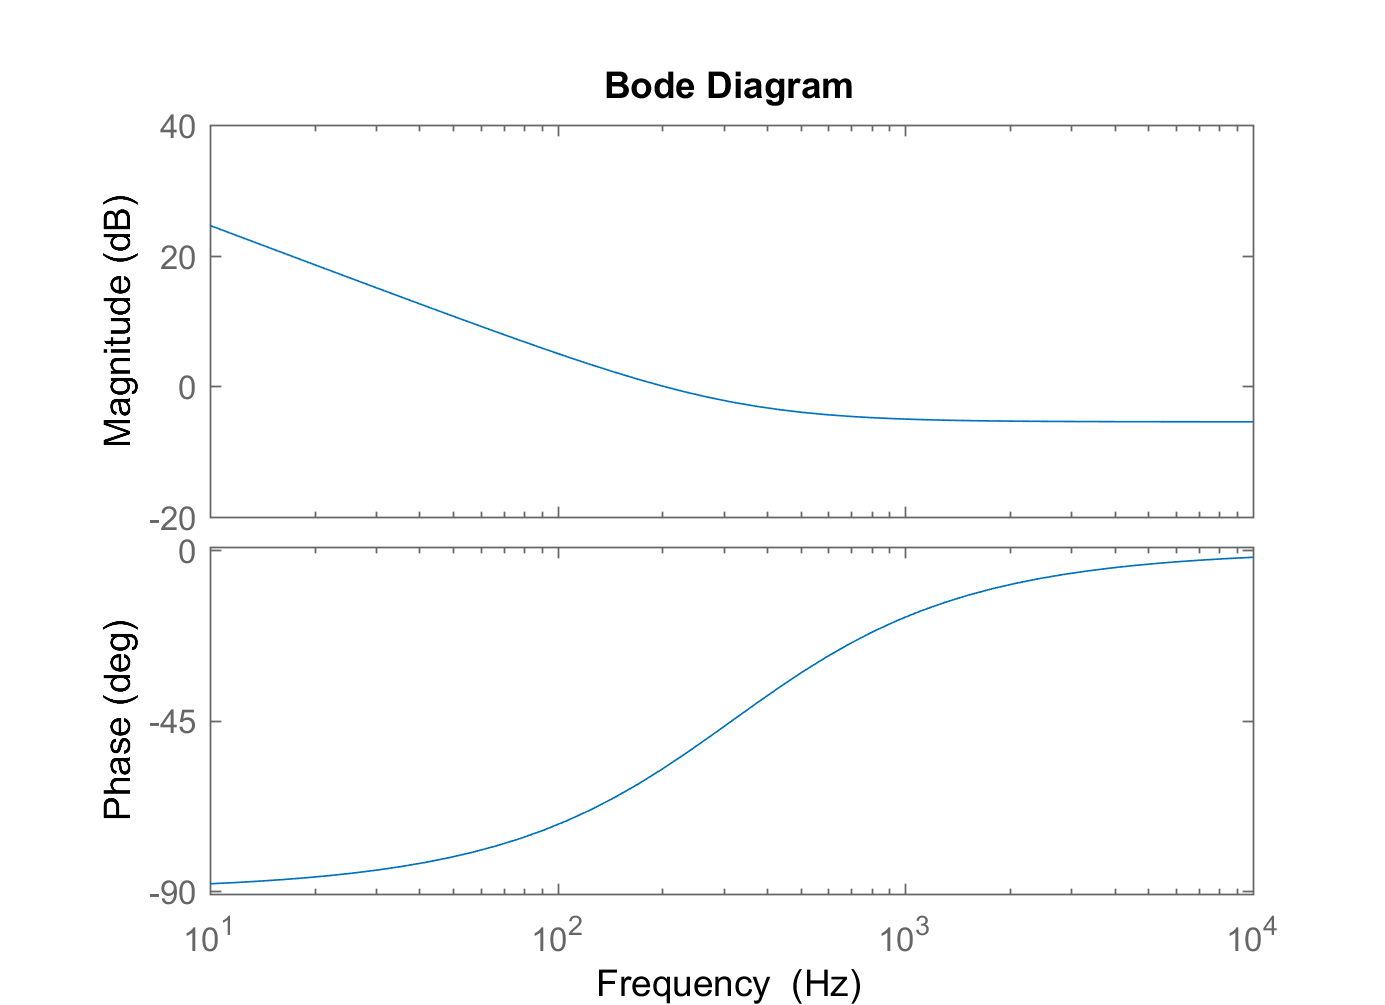
\includegraphics[max width=0.7\linewidth]{/tex/2iteration/billeder/MATLAB_error_op_amp.PNG}
	\caption{Bode plot for fejlforstærker}
	\label{fig:MATLAB_error_op_amp_2}
\end{figure}

De to overføringsfunktioner ganges sammen for, at bestemme den samlede overføringsfunktion for converteren. Figur~\ref{fig:MATLAB_total_2} viser et åben sløjfe bode plot af det. Det aflæses at converteren vil have en båndbredde på $810\hertz$. Derudover aflæses fase-margin til $74.3^\circ$, og gain-margin til $24\decibel$.

\begin{figure}[H]
	\center
	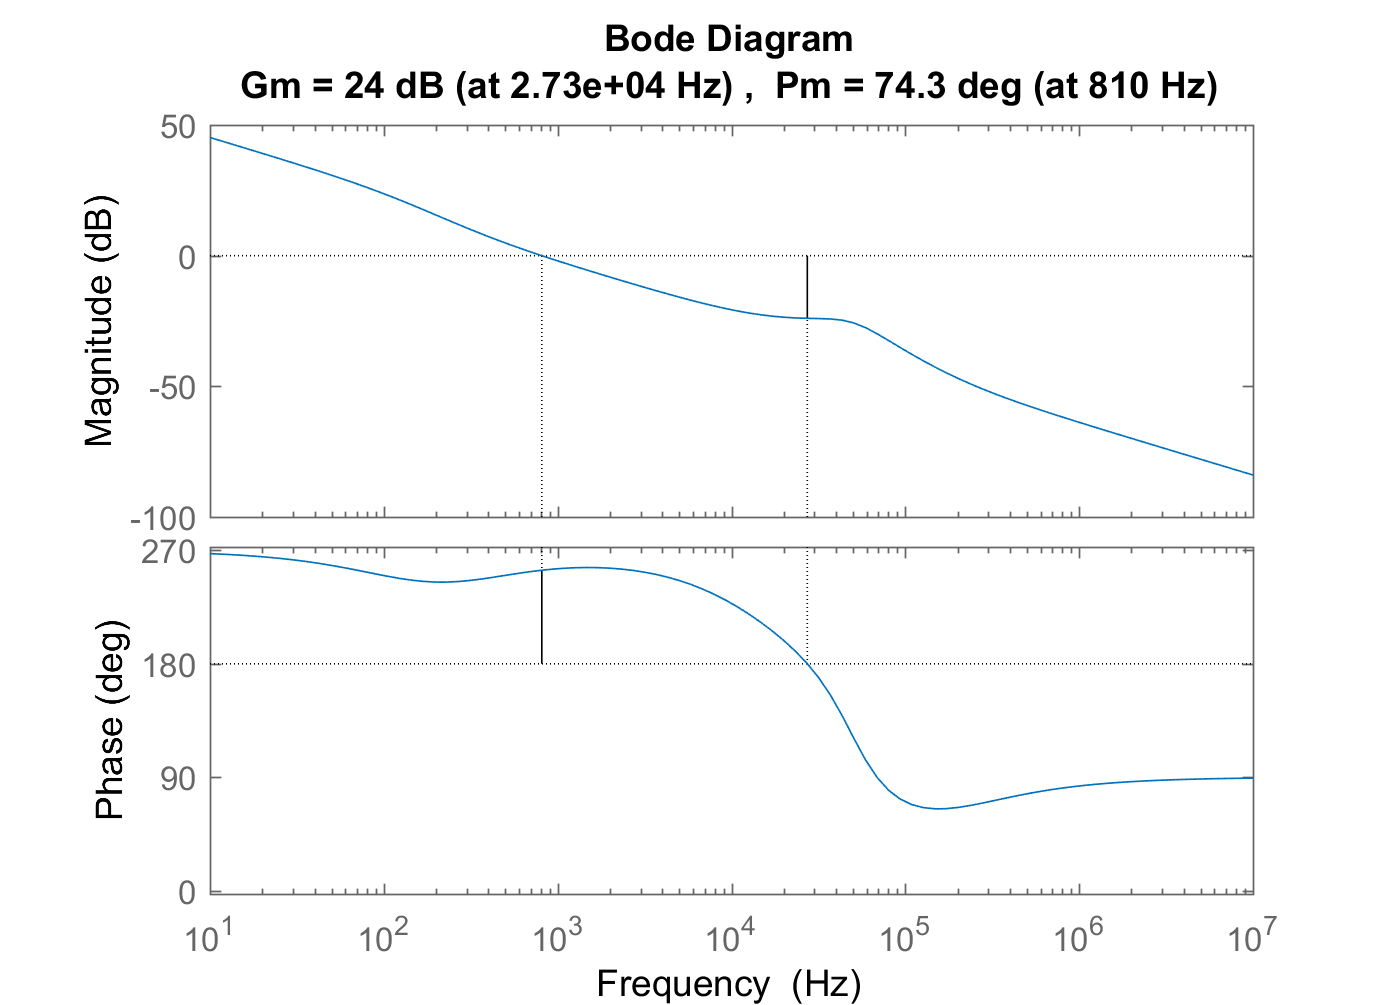
\includegraphics[max width=0.7\linewidth]{/tex/2iteration/billeder/MATLAB_total.PNG}
	\caption{Bode plot for converteren}
	\label{fig:MATLAB_total_2}
\end{figure} 





\subsection{Regulering}
Efter 2. iteration blev besluttet at optimere converterens båndbredde, da der var en stor margin til kravene for både gain- og fasemargin. Med en større båndbredde, ville der samtidig opnås en hurtigere responstid i systemet. 

For design af det nye kompensationsnetværk, blev der taget udgangspunkt i bode plottet for power-modulet. Ud fra kravene for converterens stabilitet, kunne det ses, at der kunne tilføres en forstærkning på $8.6\decibel$, og stadig overholde kravene for gain- og fasemargin. Samtidig blev knækfrekvensen for fejlforstærkeren flyttet til $132.8\hertz$, da den dominerende pol for converteren lå her. 

For at opnå den ønskede forstærkning på $8.6\decibel$, eller $2.66gg$, regnes modstanden i kompensationsnetværket til $R_{comp} = 49.8k\ohm$. For at opnå den valgte knækfrekvens regnes kondensatoren til $24.2nF$. 

For en mere detaljeret gennemgang af overføringsfunktionernes indhold, og deres bode plots, henvises til dokumentationens afsnit 6.5 og 6.8.5.


\input{tex/Implementering/2iteration/MOSdiodekon}

\section{Tab}
Dette afsnit omhandler de overvejelser, der er gjort omkring tab i 2. iteration. Her omtales hvilke bidrag, der er taget højde for, til udberegninger af tab for de enkelte komponenter. Udregningerne og yderligere forklaring af disse, kan findes dokumentationen afsnit 5.7.

\subsubsection{Transformator}
Tabet i transformatoren er set som to dele. Et kernetab og et kobbertab. Kernetabet afhænger af  kernematerialet, selvinduktionen og strømmen i viklingerne. Disse bruges til at udregne fluxen i kernen. Med denne værdi og databladskurven for det specifikke tab som funktion af maks flux massefylden, er kernetabet blevet estimeret. 

Kobbertabet kommer af modstanden, der er i kobbertrådene, som er viklet om kernen. Dette indebærer både bidrag fra en DC modstand og en AC modstand. DC modstanden er udregnet ud fra længden og tykkelsen af kobbertrådene. AC modstanden opstår på grund af magnetfeltet kobbertrådene ligger i. AC modstandens del af kobbertabet er der i dette projket ikke valgt at tage højde for.

Det samlede tab for transformatoren er testet, ved at måle temperaturen på kernen efter converteren har været i gang over længere tid. Med en datablads værdi af den termiske modstand for en RM8 kerne er tabet herefter udregnet.   

\subsubsection{MOSFET}
MOSFET'ens tab kan ligeledes deles op i to centrale bidrag; 

conduction tab og switchtab. Conduction tabet kommer af RMS strømmen der løber i MOSFET'ens ON modstand. 

Switchtabet kommer som konsekvens af effekttrekanterne, der opstår, imellem MOSFET'ens ON og OFF perioder. Effekttrekanterne er i dette projekt estimeret ved at udregne dem som arealet af to lige store trekanter. Højden på trekanten er peakaverage strømmen ganget med den maksimale spænding der vil ligge over MOSFET'en. Længden af trekanten fås af den samlede switch-tid i forhold til den samlede switch periode. 

Det samlede tab i MOSFET'en er testet ved at måle temperaturen på kølepladen efter converteren har været i gang over længere tid. Denne temperaturstigning ganget med køle-koefficienten for kølepladen giver tabet. 

\subsubsection{Diode}
Tabet i dioden er udregnet ved, at kigge på spændingsfaldet over dioden ganget udgangsstrømmen. Som nævnt benyttes en schottky diode, og der har derfor ikke været behov for betragtninger af switch-tabet i dioden. 

Tabet for dioden er fundet ved at måle temperaturen af kølepladen ligesom ved MOSFET'en ovenfor.   

\subsubsection{Kondensator}
Med en kendt ESR modstand for kondensatoren, har det været muligt at beregne tabet i denne. Da modstanden er så lille, er tabet dog uden betydning for det samlede tab.

\subsubsection{Current-sence tab}
Tabet i current-sence modstanden er udregnet ved modstandsværdien ganget med RMS strømmen i anden. Strømmen i igennem modstanden er den samme som løber i den primære vikling. 

\subsubsection{Samlet tab}
De ovenstående tab er alle analyseret og simuleret. Derudover er der lavet test af de tab, hvor det var muligt. Resultatet af dette ses i resultatafsnittet \fxnote{indsæt resultatafsnit for tab}.
Det samlede tab for converteren i 2. iteration er i analyse og simulering fundet ved at lægge de fundne tab sammen. I testen er der set på den effekt der sendes ind i converteren og trukket udgangseffekten fra denne.



\section{Integrationstest} \label{Integrationstest}
Der er lavet tre forskellige test af det samlede system, til at teste de essentielle funktioner af converteren. Det drejer sig om constant-load, gain-fase måling og load-step. For nærmere beskrivelse af hver enkelt test, henvises til dokumentationen afsnit 5.9.

På figur~\ref{fig:sche2iteration} ses et schematic for det samlede implementerede kredsløb for 2. iteration.
\begin{figure}[H]
	\center
	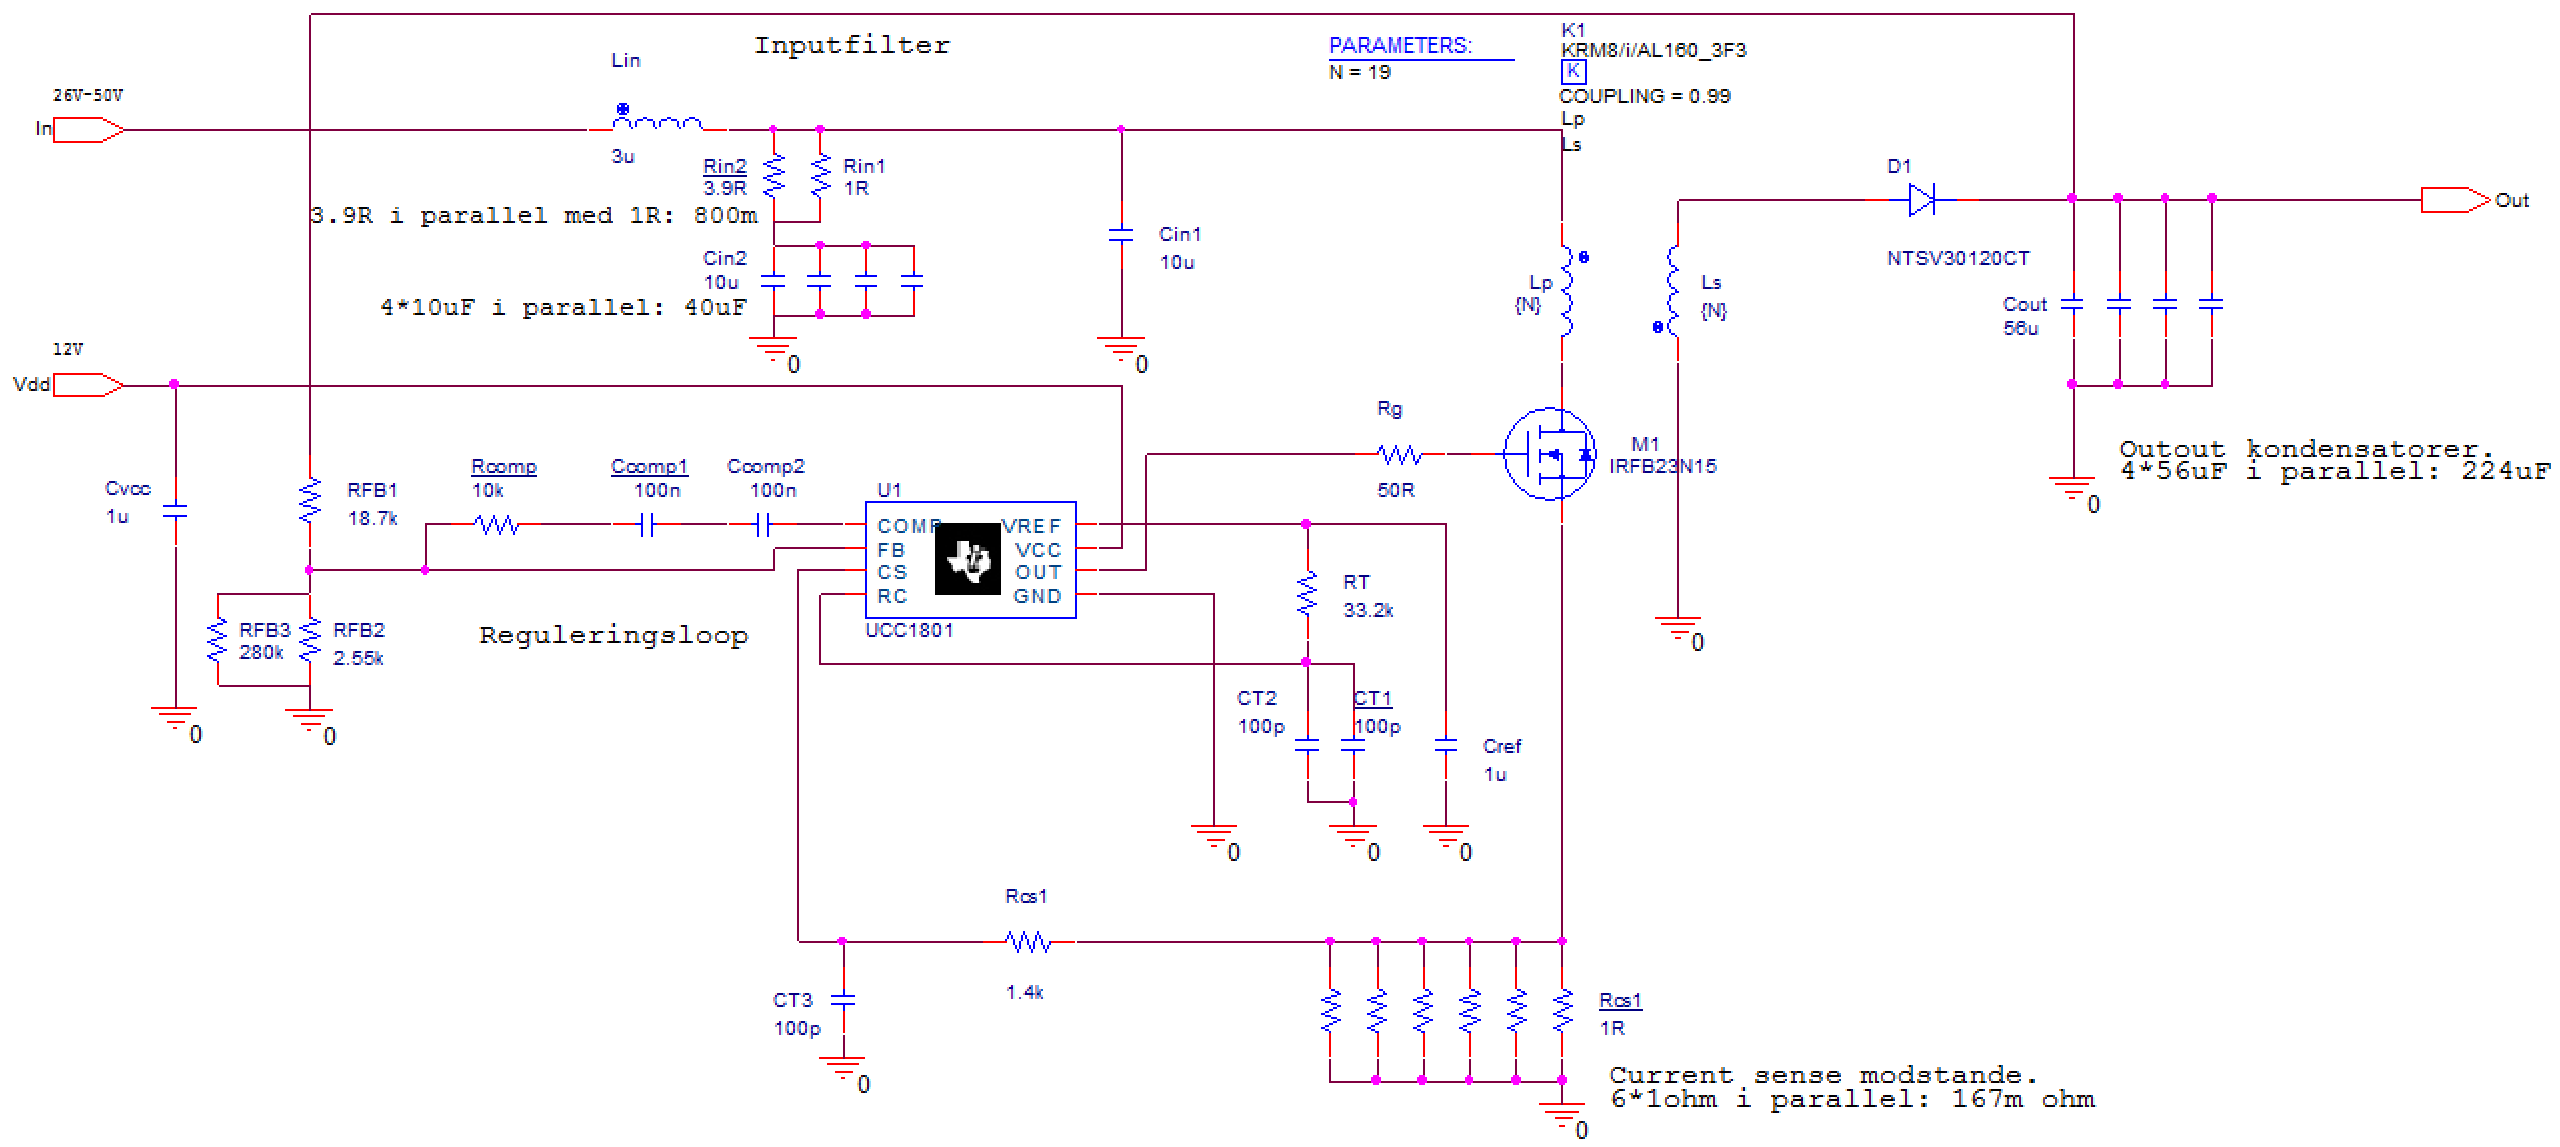
\includegraphics[max width=1.1\linewidth]{../dokumentation/tex/2iteration/billeder/Schemaricoverview_2iteration.PNG}
	\caption{Schematic overblik for 2. iteration}
	\label{fig:sche2iteration}
\end{figure}

\subsection{Constant-load}
Ved testen constant-load måles interessante steder i systemet, hvor en konstant belastning bruges. Her er en belastning på $8.4\ohm$ benyttet, med en indgangsspænding på 26V, med mindre andet er opgivet.

Ved testen er spændingen over outputtet, MOSFET'en og dioden målt. Desuden er der lavet målinger på de centrale dele af PWM-controlleren. Det indebærer målinger af switch-frekvensen, switch-tiden og stigetiden på filtret til current-sense signalet.  
Ved testen er converterens tab samtidig fundet. Tabet for transformator, MOSFET og diode er fået ved at måle temperaturen af den enkelte komponent, efter converteren har været kørende i længere tid. Temperaturstigningen er sammen med kølepladernes kølekoefficienter, og transformatorens termiske modstand, brugt til beregning af tab. Det samlede tab for converteren i 2. iteration, er i analyse og simulering fundet ved, at lægge de fundne tab sammen. I testen er der set på den effekt, der sendes ind i converteren og trukket udgangseffekten fra denne.

\subsection{Gain-fase måling}
Til gain-fase måling af converteren er Network Analyzeren HP4194A\cite{hp4194} benyttet. Her laves en måling af overføringsfunktionen for power-modul, fejlforstærker og for det samlede system. Det er gjort, ved at indføre et fejlsignal i tilbagekoblingen, og måle hvordan udgangen ændrer sig. Fejlsignalet blev indført med en amplitude på $30mV$. Dette er der lavet et frekvens-sweep på fra, $10\Hz$ til $100kHz$. Målingerne fra Network Analyzeren overføres til et Excel ark, hvor et bode plot er udarbejdet ud fra testmålingerne. 

\subsection{Load-step}
For at lave load-step testen, er der som udgangsbelastning brugt to $20\ohm$ modstande i parallel. Den ene koblet til en switch, så den kan kobles til eller fra. Det gør, at når switchen er OFF, består belastningen af en $20\ohm$ modstand. Når switchen er ON, består den i stedet af en $10\ohm$ modstand. Switchen var indstillet til at sende en puls på 10ms.

\noindent Ved denne test er det spændingsændringen på outputtet der er målt.


\clearpage

\section{Tredje iteration}
Målet for 3. iteration var, at optimere på converterens effekttab, båndbredde og udgangsens switching-spikes. Desuden blev det prioriteret at fjerne ringninger på drain- og anode spændinger, ifm. switching. Disse optimeringer er foretaget på baggrund af de diskuterede resultater fra 2. iteration i afsnit~\ref{diskussion}.
Kravet for at gå videre til 4. iteration var opnåelse af et tilfredsstillende resultat ifm. disse optimeringer.


\subsection{Switch-tid}
Efter 2. iteration blev det besluttet, at optimere effekttabet i converteren. Ud fra tabsmålingerne kunne det ses, at switch-tabet i MOSFET'en, var den dominerende faktor i det samlede effekttab. Det blev valgt, at mindske switch-tiden til lidt under en tredjedel af udgangspunktet fra 2. iteration. Det ville mindske switch-tabet betydeligt. Samtidig vil peak-spændingerne over MOSFET'en stadig overholde dens specifikationer. 

Modstanden, der skulle sikre den hurtigere switch-tid, blev designet efter samme formel som i 2.iteration. Den blev regnet til $13.7\ohm$, hvilket gav en switch-tid på ca. $37.2ns$. 

En nærmere beskrivelse af konsekvenser og designmetode, er beskrevet i dokumentationen, afsnit 6.1.


\subsection{Current-sense filter}
Efter 2. iteration blev det valgt, at optimere stigetiden i current-sense filteret. Det blev gjort for, at fjerne fejlmålinger af strømmen i primærviklingen, og dermed forbedre converterens I/V-karakteristik. 

Ved aflæsning af bredden på spikes på current-sense signalet, blev det valgt, at designe filteret til en stigetid på $100ns$. Ved at fastholde kondensatoren i filteret på $100pF$, blev den nye modstand regent til $464\ohm$. 

En nærmere begrundelse for designvalg og -metode er beskrevet i dokumentationens afsnit 6.2.


\subsection{Snubber-kredsløb}
Der blev designet to snubber-kredsløb for, at fjerne ringninger på spændingen over både MOSFET og diode. De blev anslået som en konsekvens af, at spredningsselvinduktionen fremstår som en serieforbindelse med kapaciteterne over henholdsvis MOSFET'en, dioden og den kapacitive kobling mellem transformatorens viklinger.  

Det blev valgt, at implementere RC-snubbere til både primær- og sekundærsiden. De består af en modstand i serie med en kondensator, som skal placeres over henholdsvis MOSFET og diode. 

Med kendskab til ringningernes frekvens på primærsiden og transformatorens spredningsselvinduktion, blev den resulterende kapacitet regnet til $266.6pF$. Kondensatoren i snubber-kredsløbet blev valgt til en faktor 2 større, end den resulterende kapacitet, for optimal funktionalitet\cite{snubber_design}. Modstanden blev designet således, at dens impedansen var lig impedansen af spredningsselvinduktionen ved ringningsfrekvensen. Hermed blev snubber-kredsløbet designet til $C_{snubM} = 600pF$ og $R_{snubM} = 23.7\ohm$. 

Figur~\ref{fig:snubber_diagram} viser implementeringen af de to snubber-kredsløb. Her vises de specifikke komponentværdier og placeringen af de to kredsløbene.

\begin{figure}[H]
	\centering
	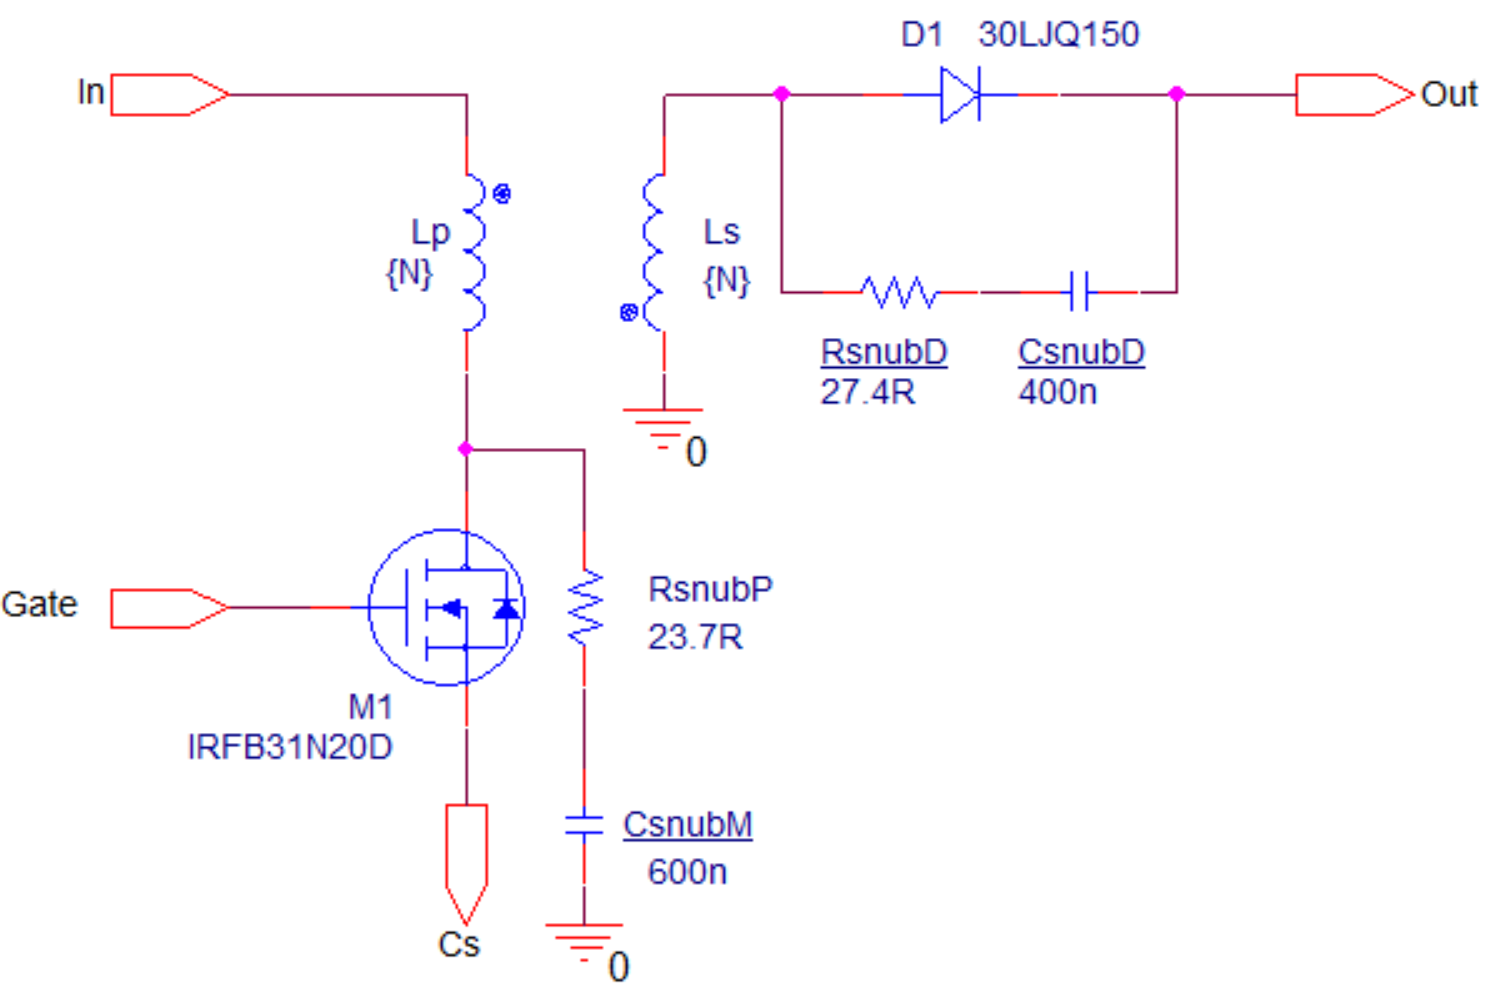
\includegraphics[width=0.4\linewidth]{/tex/Implementering/3iteration/Billeder/Snubber_diagram.png}
	\caption{P-spice diagram for snubber-kredsløb}
	\label{fig:snubber_diagram}
\end{figure}

\noindent Designmetoden for snubber-kredsløbet på sekundærsiden er den samme. Der findes en detaljeret gennemgang af designproceduren og en argumentation for valg af snubber-type i dokumentationen, afsnit 6.3.



\subsection{Udgangsfilter}
I 2. iteration blev det observeret store switching-spikes på udgangssignalet. Derfor blev det besluttet, at tilførere filtrering af disse spikes i 3. iteration. Den nødvendige kapacitet for udgangskondensatoren, blev realiseret ved fire kondensatorer i parallel. Kondensatorerne blev forbundet med ledninger på ca. $30mm$, ses på figur~\ref{fig:udgangsfilter}. Med en tommelfinger regel der siger man har selvinduktion på $1nH/mm$\cite{rule_of_thumb}, vil ledningerne og kondensatorerne derfor skabe fire LC-filtre i serie. Ved at placere udgangen efter disse filtre blev der derfor opnået en filtrering af spikes'ne uden yderligere tilføjelse af komponenter. 

\begin{figure}[H]
	\centering
	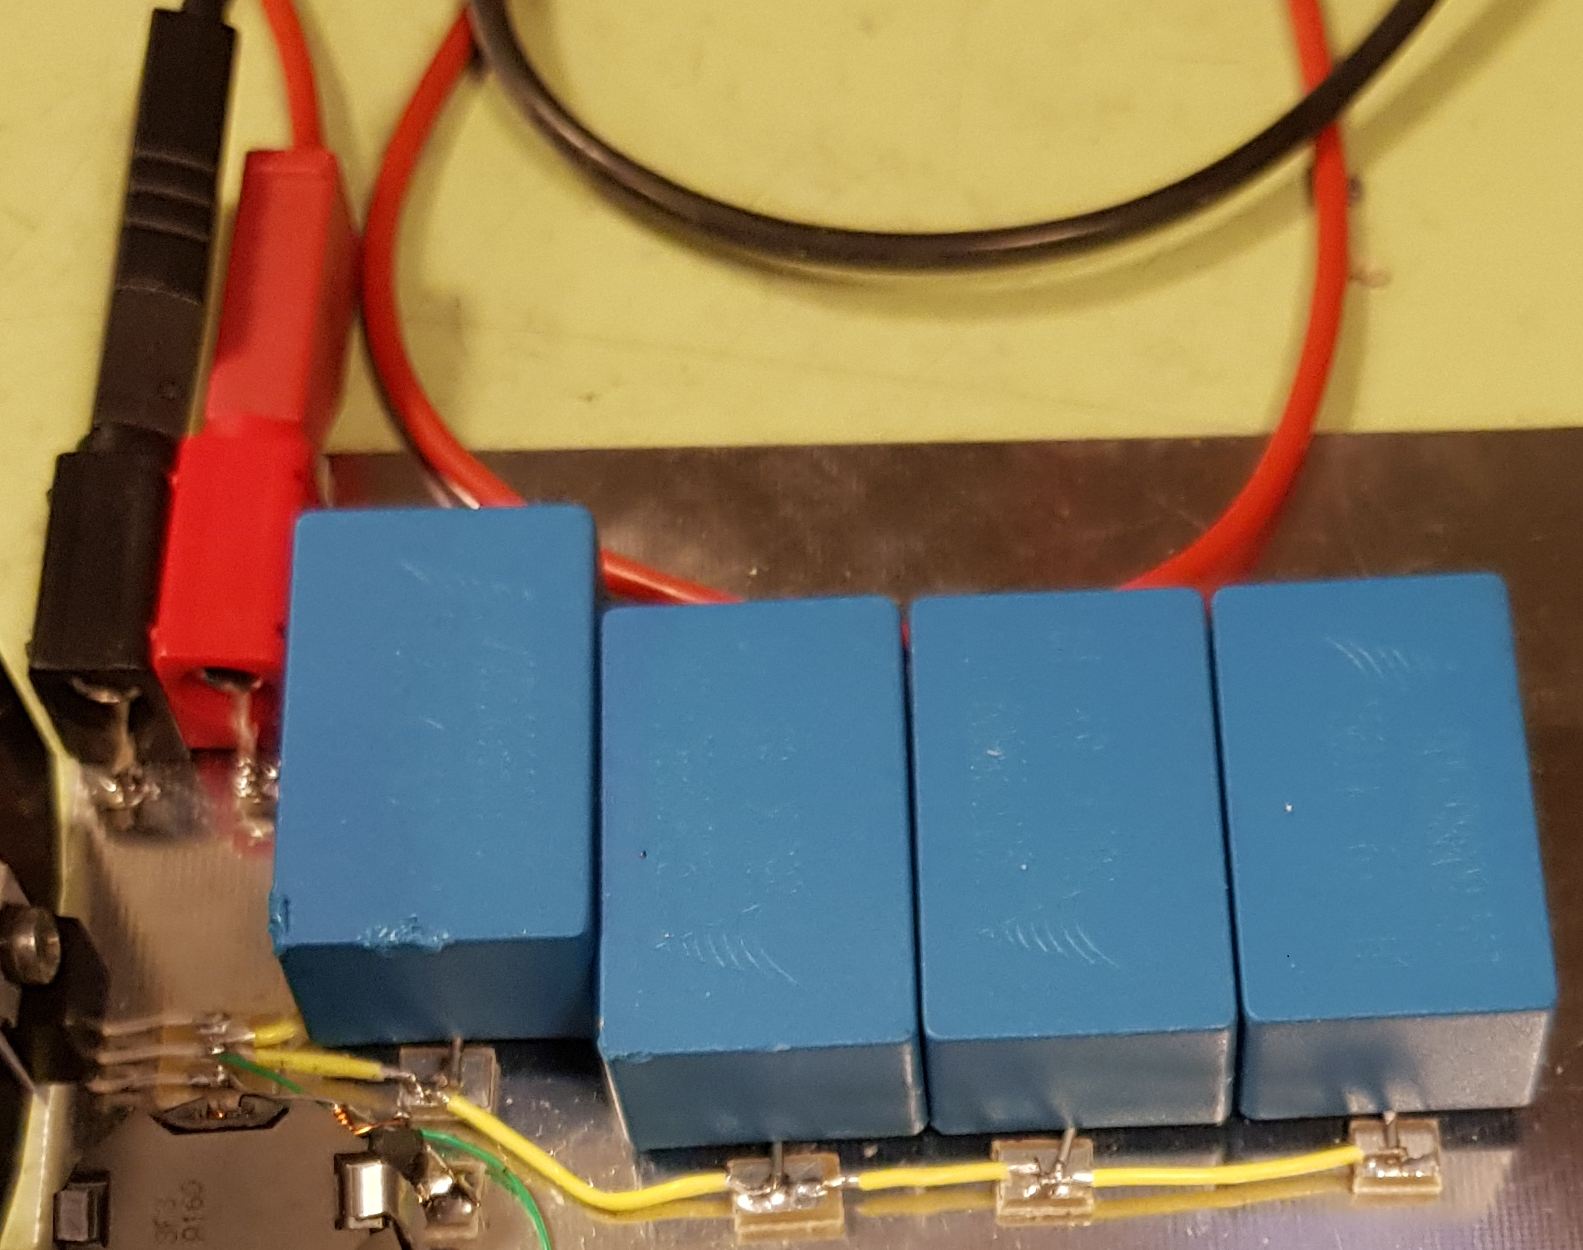
\includegraphics[width=0.5\linewidth]{../Dokumentation/tex/3iteration/Billeder/Analyse/Udgangsfilter_2iteration.png}
	\caption{Realisering af udgangsfilter efter 2. iteration}
	\label{fig:udgangsfilter}
\end{figure}

\noindent En nærmere analyse af udgangsfilteret er beskrevet i dokumentationens afsnit 6.4.


\subsection{Regulering}
Efter 2. iteration blev besluttet at optimere converterens båndbredde, da der var en stor margin til kravene for både gain- og fasemargin. Med en større båndbredde, ville der samtidig opnås en hurtigere responstid i systemet. 

For design af det nye kompensationsnetværk, blev der taget udgangspunkt i bode plottet for power-modulet. Ud fra kravene for converterens stabilitet, kunne det ses, at der kunne tilføres en forstærkning på $8.6\decibel$, og stadig overholde kravene for gain- og fasemargin. Samtidig blev knækfrekvensen for fejlforstærkeren flyttet til $132.8\hertz$, da den dominerende pol for converteren lå her. 

For at opnå den ønskede forstærkning på $8.6\decibel$, eller $2.66gg$, regnes modstanden i kompensationsnetværket til $R_{comp} = 49.8k\ohm$. For at opnå den valgte knækfrekvens regnes kondensatoren til $24.2nF$. 

For en mere detaljeret gennemgang af overføringsfunktionernes indhold, og deres bode plots, henvises til dokumentationens afsnit 6.5 og 6.8.5.


\section{Tab}
Dette afsnit omhandler de overvejelser, der er gjort omkring tab i 2. iteration. Her omtales hvilke bidrag, der er taget højde for, til udberegninger af tab for de enkelte komponenter. Udregningerne og yderligere forklaring af disse, kan findes dokumentationen afsnit 5.7.

\subsubsection{Transformator}
Tabet i transformatoren er set som to dele. Et kernetab og et kobbertab. Kernetabet afhænger af  kernematerialet, selvinduktionen og strømmen i viklingerne. Disse bruges til at udregne fluxen i kernen. Med denne værdi og databladskurven for det specifikke tab som funktion af maks flux massefylden, er kernetabet blevet estimeret. 

Kobbertabet kommer af modstanden, der er i kobbertrådene, som er viklet om kernen. Dette indebærer både bidrag fra en DC modstand og en AC modstand. DC modstanden er udregnet ud fra længden og tykkelsen af kobbertrådene. AC modstanden opstår på grund af magnetfeltet kobbertrådene ligger i. AC modstandens del af kobbertabet er der i dette projket ikke valgt at tage højde for.

Det samlede tab for transformatoren er testet, ved at måle temperaturen på kernen efter converteren har været i gang over længere tid. Med en datablads værdi af den termiske modstand for en RM8 kerne er tabet herefter udregnet.   

\subsubsection{MOSFET}
MOSFET'ens tab kan ligeledes deles op i to centrale bidrag; 

conduction tab og switchtab. Conduction tabet kommer af RMS strømmen der løber i MOSFET'ens ON modstand. 

Switchtabet kommer som konsekvens af effekttrekanterne, der opstår, imellem MOSFET'ens ON og OFF perioder. Effekttrekanterne er i dette projekt estimeret ved at udregne dem som arealet af to lige store trekanter. Højden på trekanten er peakaverage strømmen ganget med den maksimale spænding der vil ligge over MOSFET'en. Længden af trekanten fås af den samlede switch-tid i forhold til den samlede switch periode. 

Det samlede tab i MOSFET'en er testet ved at måle temperaturen på kølepladen efter converteren har været i gang over længere tid. Denne temperaturstigning ganget med køle-koefficienten for kølepladen giver tabet. 

\subsubsection{Diode}
Tabet i dioden er udregnet ved, at kigge på spændingsfaldet over dioden ganget udgangsstrømmen. Som nævnt benyttes en schottky diode, og der har derfor ikke været behov for betragtninger af switch-tabet i dioden. 

Tabet for dioden er fundet ved at måle temperaturen af kølepladen ligesom ved MOSFET'en ovenfor.   

\subsubsection{Kondensator}
Med en kendt ESR modstand for kondensatoren, har det været muligt at beregne tabet i denne. Da modstanden er så lille, er tabet dog uden betydning for det samlede tab.

\subsubsection{Current-sence tab}
Tabet i current-sence modstanden er udregnet ved modstandsværdien ganget med RMS strømmen i anden. Strømmen i igennem modstanden er den samme som løber i den primære vikling. 

\subsubsection{Samlet tab}
De ovenstående tab er alle analyseret og simuleret. Derudover er der lavet test af de tab, hvor det var muligt. Resultatet af dette ses i resultatafsnittet \fxnote{indsæt resultatafsnit for tab}.
Det samlede tab for converteren i 2. iteration er i analyse og simulering fundet ved at lægge de fundne tab sammen. I testen er der set på den effekt der sendes ind i converteren og trukket udgangseffekten fra denne.



\section{Integrationstest} \label{Integrationstest}
Der er lavet tre forskellige test af det samlede system, til at teste de essentielle funktioner af converteren. Det drejer sig om constant-load, gain-fase måling og load-step. For nærmere beskrivelse af hver enkelt test, henvises til dokumentationen afsnit 5.9.

På figur~\ref{fig:sche2iteration} ses et schematic for det samlede implementerede kredsløb for 2. iteration.
\begin{figure}[H]
	\center
	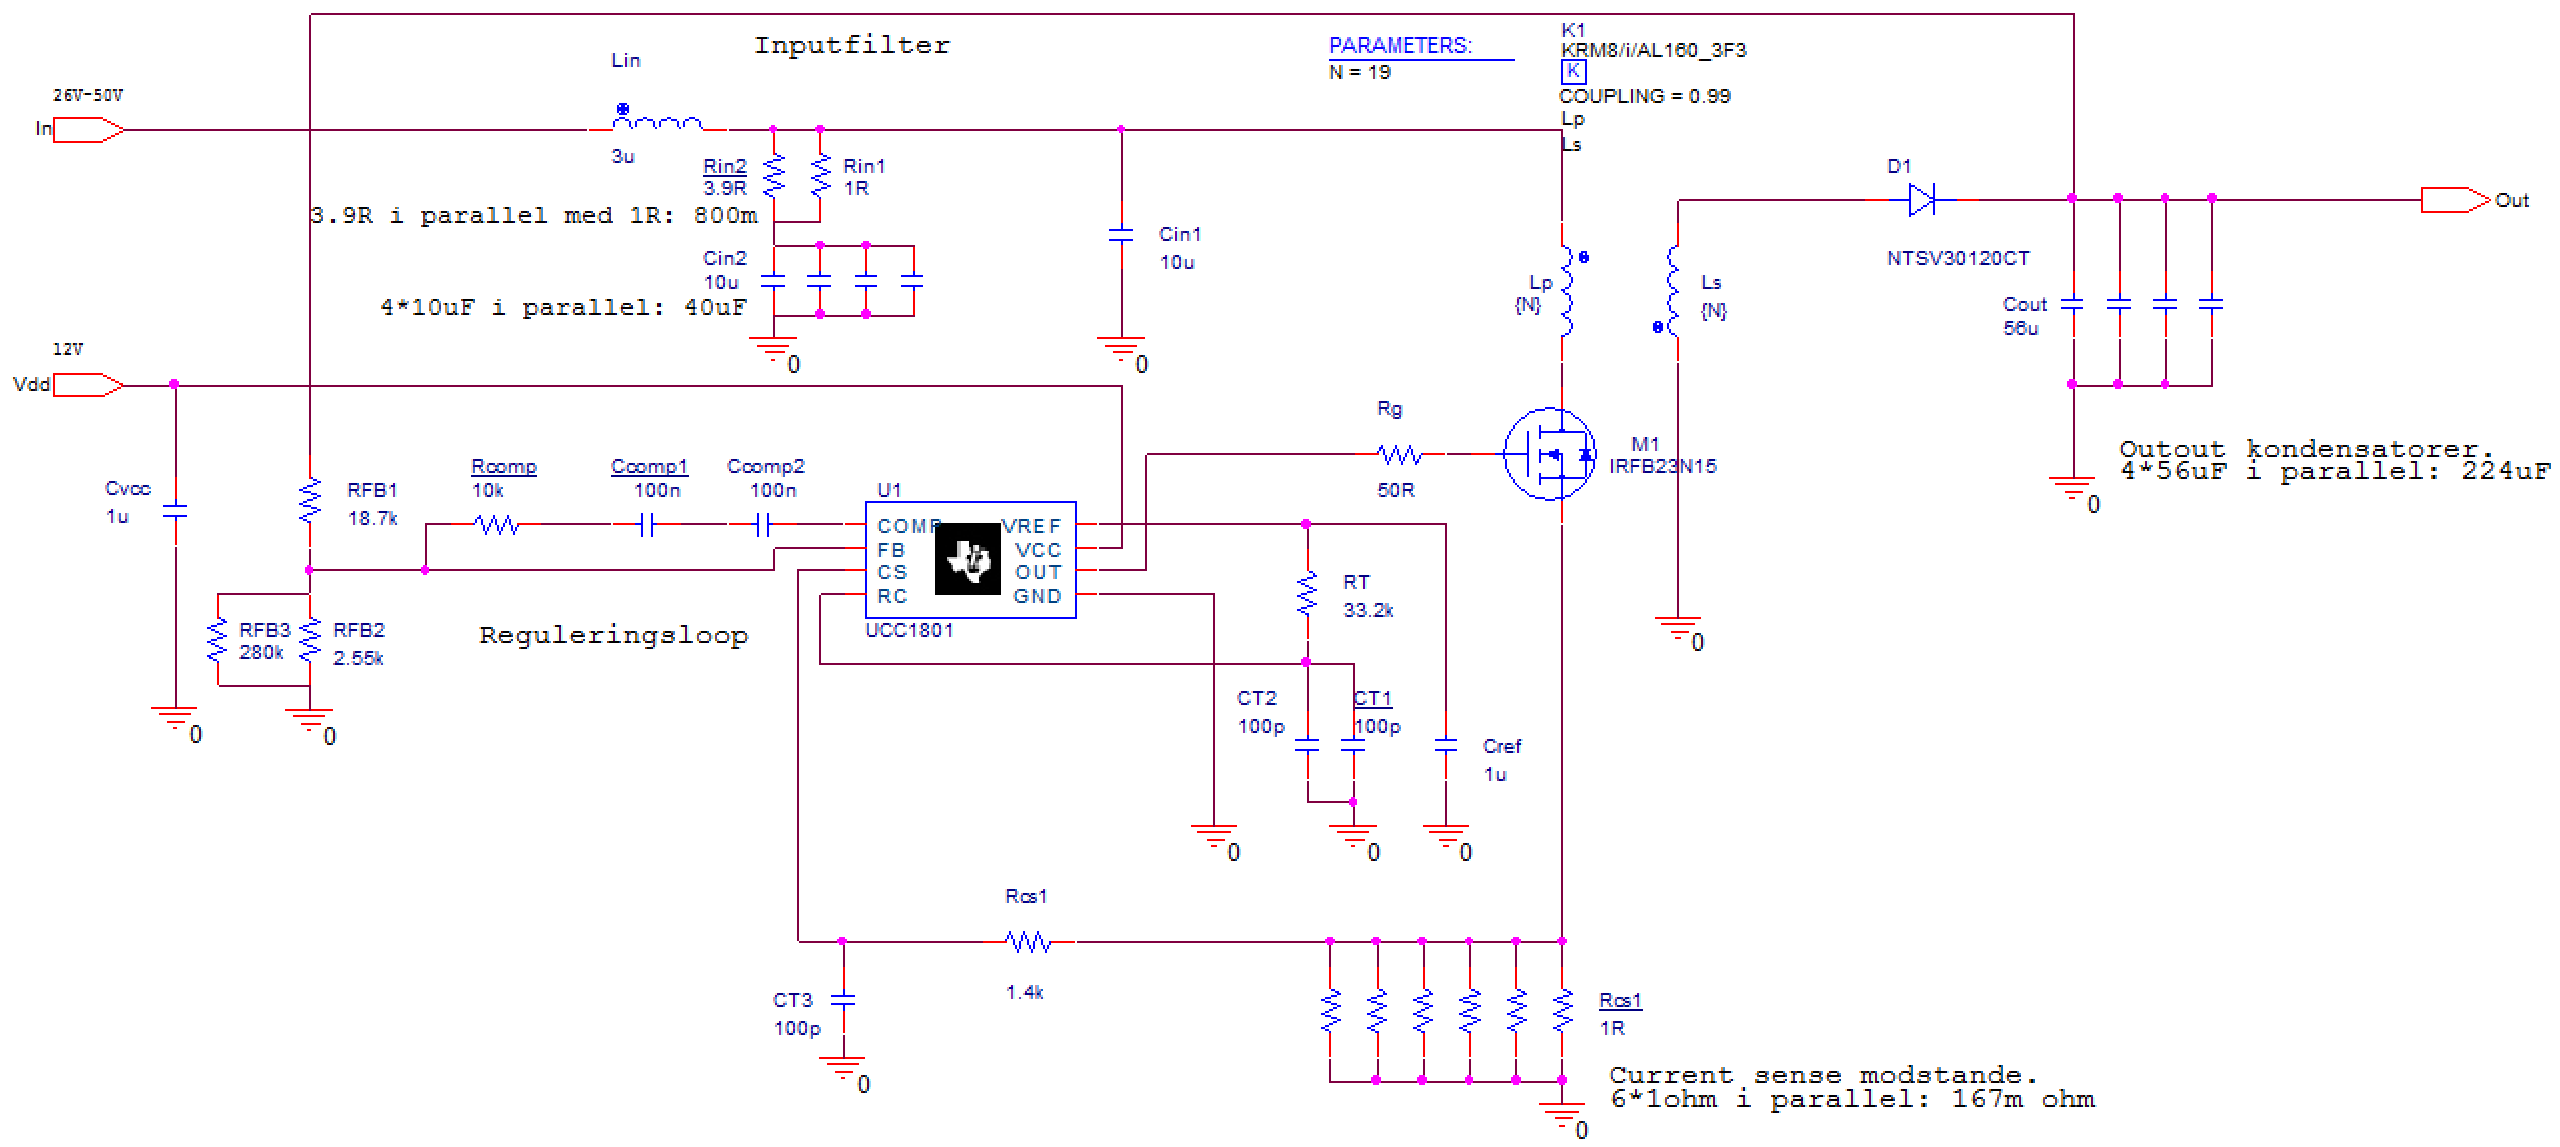
\includegraphics[max width=1.1\linewidth]{../dokumentation/tex/2iteration/billeder/Schemaricoverview_2iteration.PNG}
	\caption{Schematic overblik for 2. iteration}
	\label{fig:sche2iteration}
\end{figure}

\subsection{Constant-load}
Ved testen constant-load måles interessante steder i systemet, hvor en konstant belastning bruges. Her er en belastning på $8.4\ohm$ benyttet, med en indgangsspænding på 26V, med mindre andet er opgivet.

Ved testen er spændingen over outputtet, MOSFET'en og dioden målt. Desuden er der lavet målinger på de centrale dele af PWM-controlleren. Det indebærer målinger af switch-frekvensen, switch-tiden og stigetiden på filtret til current-sense signalet.  
Ved testen er converterens tab samtidig fundet. Tabet for transformator, MOSFET og diode er fået ved at måle temperaturen af den enkelte komponent, efter converteren har været kørende i længere tid. Temperaturstigningen er sammen med kølepladernes kølekoefficienter, og transformatorens termiske modstand, brugt til beregning af tab. Det samlede tab for converteren i 2. iteration, er i analyse og simulering fundet ved, at lægge de fundne tab sammen. I testen er der set på den effekt, der sendes ind i converteren og trukket udgangseffekten fra denne.

\subsection{Gain-fase måling}
Til gain-fase måling af converteren er Network Analyzeren HP4194A\cite{hp4194} benyttet. Her laves en måling af overføringsfunktionen for power-modul, fejlforstærker og for det samlede system. Det er gjort, ved at indføre et fejlsignal i tilbagekoblingen, og måle hvordan udgangen ændrer sig. Fejlsignalet blev indført med en amplitude på $30mV$. Dette er der lavet et frekvens-sweep på fra, $10\Hz$ til $100kHz$. Målingerne fra Network Analyzeren overføres til et Excel ark, hvor et bode plot er udarbejdet ud fra testmålingerne. 

\subsection{Load-step}
For at lave load-step testen, er der som udgangsbelastning brugt to $20\ohm$ modstande i parallel. Den ene koblet til en switch, så den kan kobles til eller fra. Det gør, at når switchen er OFF, består belastningen af en $20\ohm$ modstand. Når switchen er ON, består den i stedet af en $10\ohm$ modstand. Switchen var indstillet til at sende en puls på 10ms.

\noindent Ved denne test er det spændingsændringen på outputtet der er målt.


%%% Første iteration
	% Converter
	
%%% Anden iteration
	% Transformator
	% PWM controller
	% MOSFET, diode og udgangsfilter
	% Regulering
	% Tab
	
%%% Tredje iteration
	% Snubber
	% Switch-tid
	% Udgangsfilter
	% Regulering
	% Tab

	\chapter{Resultater}
I dette kapitel er de vigtigste resultater for hver af iterationerne vist. Detaljeret dokumentation af resultaterne kan findes i dokumentationen i afsnit 4, 5 og 6. 

% Dokumentation af converter topologi

\chapter{Første Iteration}
I dette afsnit beskrives den indledende og første iteration af designfasen. Den indebærer valg af converter topologi, samt simulering af en ideel converter.

\section{Switch Mode Power-Supply}
I dette projekt vælges der at tage udgangspunkt i Switch Mode Power-Supply (SMPS). Da der er stillet et krav om et maksimalt tab på 5W, betyder det, ved en maksimal udgangseffekt på 75W, at converteren skal have en effektivitet på:
\begin{equation}
	\eta = \frac{75W}{75W + 5W} \cdot 100 = 93.75\percent
\end{equation}

En lineær converter vil ofte have en effektivitet på mellem $30-40\percent$. Da dette ikke vil kunne efterleve kravet på $93.75\percent$, udelukkes de lineære convertere. Dette kan til gengæld tilnærmes ved brug af en SMPS. Ved optimering af tabene i converteren, kan man opnå en effektivitet på op mod $95\percent$\cite{smps}.


\section{Buck Converter}
En simpel converter der bruges til nedregulering af en spænding, er buck converteren. Den består af en transistor, der er placeret i serie med et lavpas filter, i form af et LC-filter. Derudover er der placeret en diode før filteret, således strømmen i spolen har en løbevej, når transistoren går OFF. Det overordnede kredsløb for en buck converter er vist på figur~\ref{fig:buck_converter_circuit}.


\begin{figure}[H]
	\center
	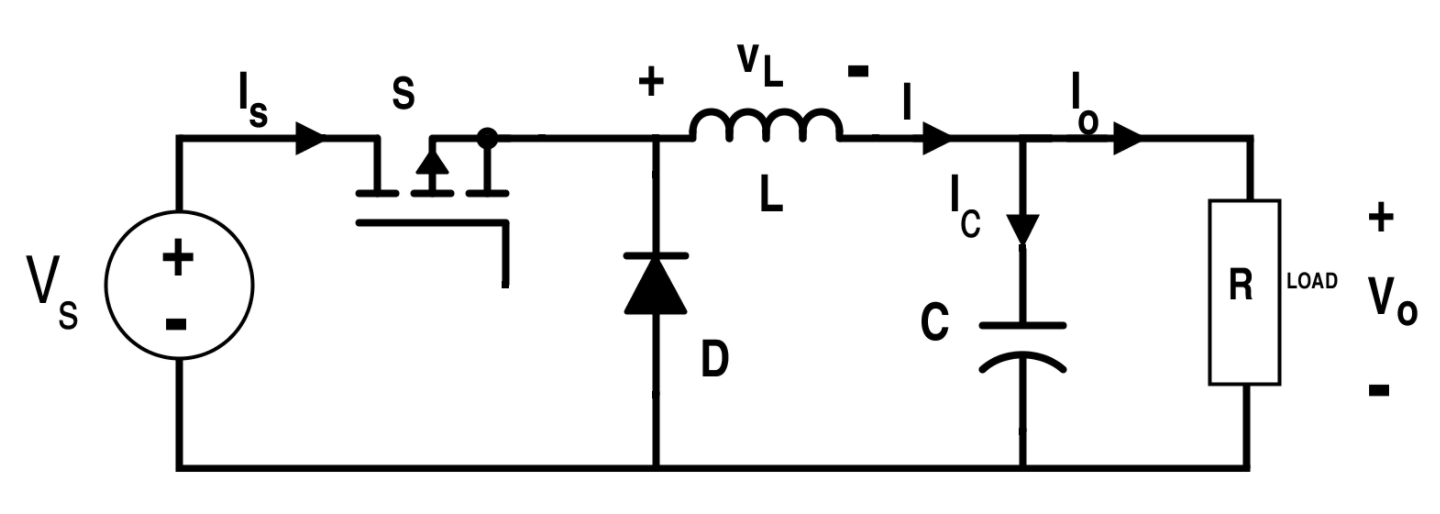
\includegraphics[max width=0.7\linewidth]{/tex/1iteration/billeder/Buck_converter_circuit.PNG}
	\caption{Ideelt diagram af buck converteren
		\cite{buck-converter}}
	\label{fig:buck_converter_circuit}
\end{figure}


I transistorens ON tid, vil strømmen i spolen, og dermed også strømmen i transistoren, rampe op. Det gør den, da der er en positiv spænding over spolen. Den spænding er lig $V_L=V_S-V_O$. Når der er et positivt spændingsfald over spolen, vil dioden være forspændt i spærreretningen, og dermed ikke lede en strøm. Når transistoren går OFF, vil strømmen begynde at løbe gennem dioden, da strømmen i en spole ikke kan skifte momentant. Hvis vi ser dioden som ideel, vil spændingen over spolen nu være lig $V_L=0-V_O$. Da dette giver et negativt spændingsfald over spolen, vil strømmen begynde at aflade i den. Strømmene er skitseret på figur~\ref{fig:buck_converter_current}. Her ses det, at der altid løber en strøm i spolen, mens den skiftes til at løbe i transistoren og dioden, afhængig af ON og OFF perioderne. 


\begin{figure}[H]
	\center
	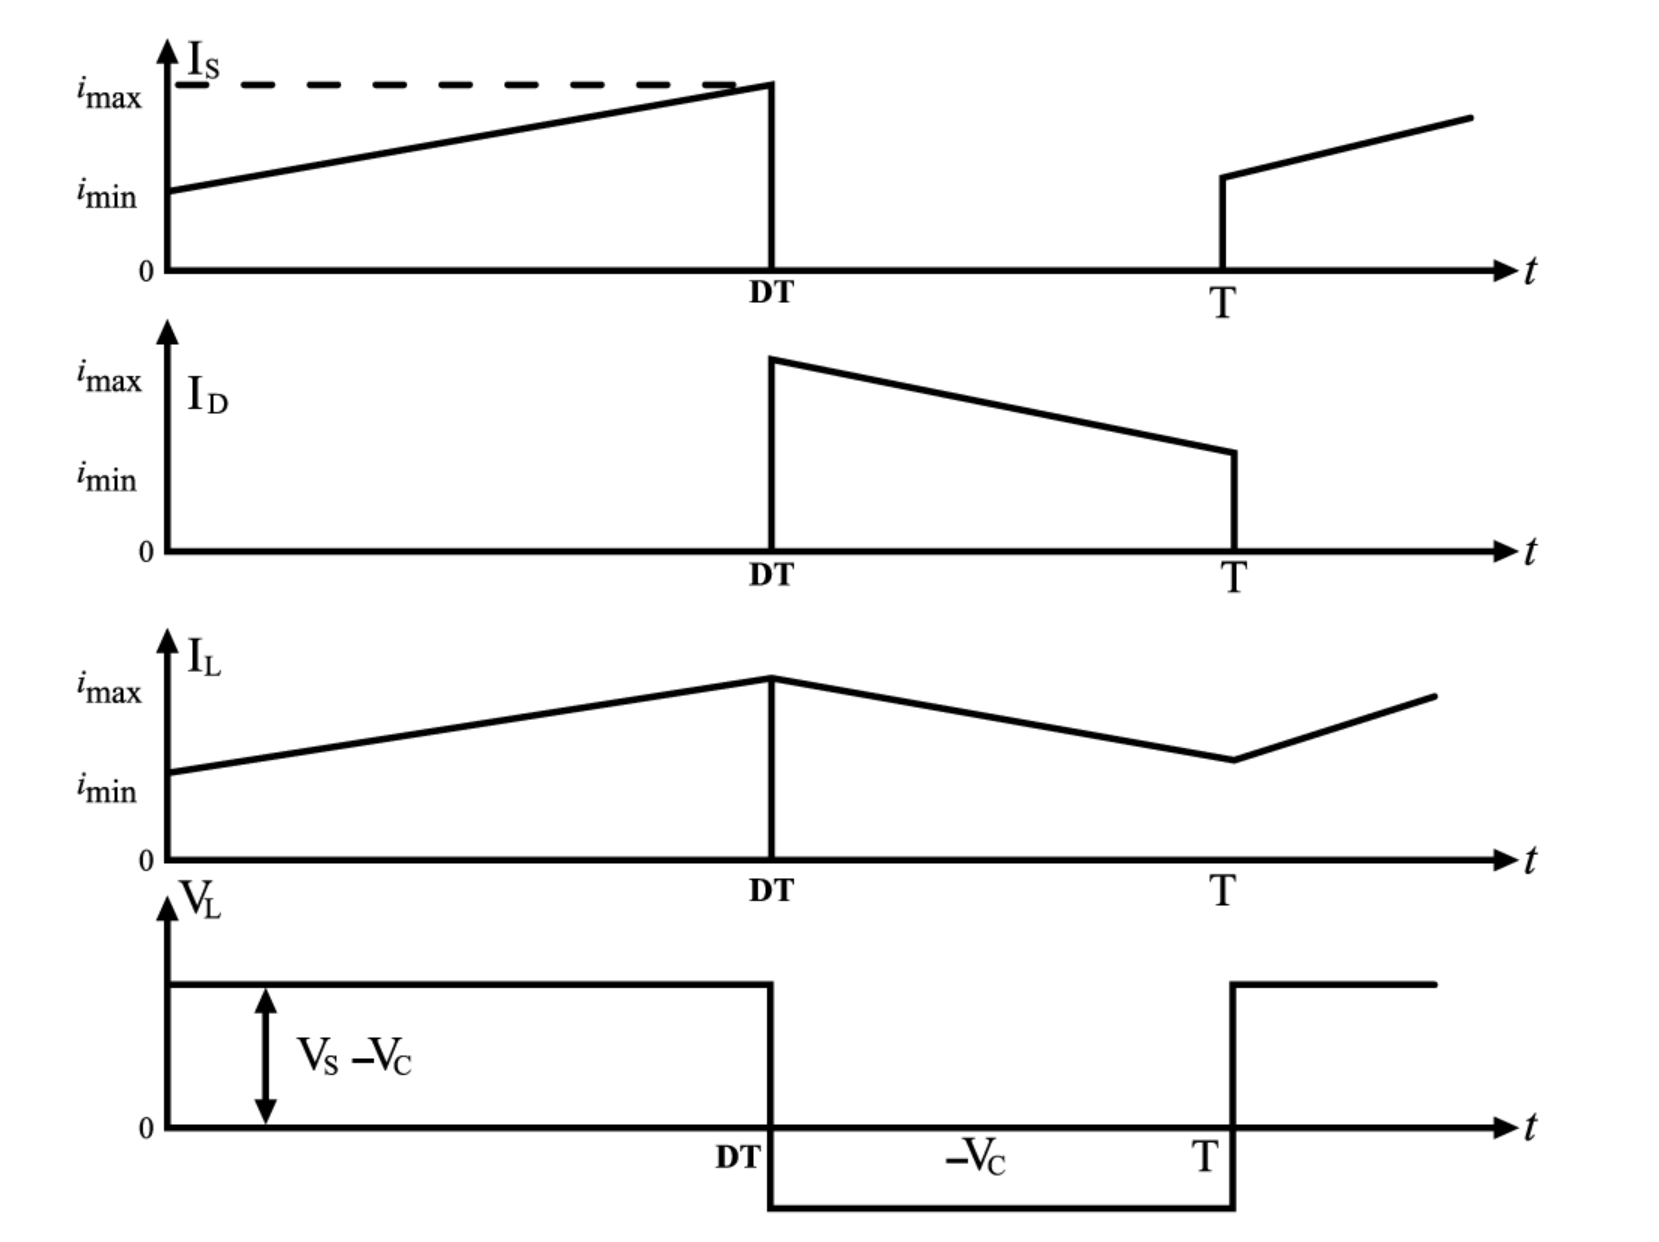
\includegraphics[max width=0.7\linewidth]{/tex/1iteration/billeder/Buck_converter_current.PNG}
	\caption{Buck converter strømme
		\cite{buck-converter}}
	\label{fig:buck_converter_current}
\end{figure}


Da strømmen i spolen aldrig når $0A$, kaldes denne form for operation Continuous Conduction Mode, eller CCM. Overføringsfunktionen for en buck converter i CCM er\cite{SMPS-topologies}:
\begin{equation} \label{buck_converter_overforinsfunktion}
V_{out} = D\cdot V_{in}
\end{equation}

Converteren skal kunne opretholde en outputspænding på $21V$, ved en inputspænding på $26V$. Ved at bruge overføringsfunktionen, regnes den maksimale duty-cycle til ca. $80\percent$. 

En af fordelene ved buck converteren, er at der altid løber en strøm i spolen. Dette gør, at der kan opnås en lille ripple-strøm i filteret, og derved også et mindre tab, både i spolen og kondensatoren. 
En af ulemperne, er at transistoren sidder i den positive forsyningslinje. Dette Kan give komplikationer ved switching af transistoren. Hvis der vælges en p-kanals MOSFET, skal der vælges en PWM-controller der kan håndtere switching af denne. Hvis der vælges en n-kanals MOSFET, skal gate signalet være større end forsyningen, før MOSFET'en er helt ON. Dette kræver flere komponenter, og vil derfor helst undgås. På grund af dette problem undersøges der en converter topologi, hvor MOSFET'en ikke sidder i den positive forsyningslinje.

\section{Flyback Converter}
Flyback converteren, er en transformator baseret topologi. Man deler converteren op i to dele: Primær- og sekundærsiden. Primærsiden består af primærviklingen af transformatoren og en transistor, hvor transistoren fungerer som en switch. Sekundærsiden består af sekundærviklingen, en diode, en udgangskondensator og belastningen. Dette er vist på figur~\ref{fig:flyback_ideal}. En af fordelene ved, at bruge flyback converteren, er at der kan opnås galvanisk adskillelse mellem primær- og sekundærsiden af transformatoren, samt MOSFET'ens source er forbundet til GND. Derudover bruges der det samme antal komponenter, som ved buck converteren.

\begin{figure}[H]
	\center
	\includegraphics[max width=0.7\linewidth]{/tex/1iteration/billeder/flyback_ideal.PNG}
	\caption{Ideelt diagram af flyback converteren
	\cite{SMPS-topologies}}
	\label{fig:flyback_ideal}
\end{figure} 

\noindent Flyback converteren bruges til at konvertere en indgangsspænding, ned til en mindre udgangsspænding. Dette gøres ved at styre transistoren med et PWM-signal, med en variabel duty-cycle. Når den er ON, vil der være en positiv spænding ved prik-enden af viklingen ift. den anden ende. Ud fra formlen $V=L\cdot \frac{di}{dt}$ kan det ses, at når der ligger en spænding over viklingen, vil strømmen i transformatoren stige lineært, over den tid transistoren er ON. Når transistoren går OFF, vil den magnetiske strøm i transformatoren inducere en spænding over sekundærviklingen. Når denne spænding bliver lig udgangsspændingen, vil dioden begynde at lede den strøm, der er oplagret i transformatoren. Da spændingen over sekundærviklingen er positiv ved prikken, og dermed modsat af primærviklingen, vil strømmen falde lineært ud fra samme forhold, som nævnt tidligere. Dette vil over tid skabe en trekantet kurveform af den samlede strøm i transformatoren. Et eksempel på dette kan ses på figur \ref{fig:CCM_transformer_current}. Da strømmen i hver vikling er diskontinuert, vil det give anledning til større peak-strømme. Det er maksimalt $50\percent$ af tiden der løber en strøm i viklingen, hvilket betyder en større strøm for at opretholde den samme middelstrøm.

Flyback converteren kan overordnet drives på to forskellige måder, Continuous Conduction Mode (CCM) og Discontinuous Conduction Mode (DCM). Disse to måder har forskellige fordele og ulemper, som skal tages højde for inden der vælges hvordan converteren skal drives. 

\subsection{Continuous Conduction Mode}
Forkellen ved CCM og DCM er, hvordan strømmen løber i transformatoren. Ved CCM vil der altid løbe en strøm i transformatoren, som der også ligger i navnet. Dog vil strømmene individuelt i viklingerne være diskontinuerte. Strømmen er skitseret på figur \ref{fig:CCM_transformer_current}. Skal man have den samlede strøm i transformatoren, skal de to kurver for primær- og sekundærviklingen samles. Dette er fordi der kun løber en strøm i primærviklingen når transistoren er ON, og en strøm i sekundærviklingen når transistoren er OFF. 

\noindent Overføringsfunktionen for en flyback converter i CCM er\cite{SMPS-topologies}:
\begin{equation} \label{flyback_converter_CCM_overforinsfunktion}
V_{out} = \frac{N_S}{N_P} \cdot \frac{D}{1-D} \cdot V_{in}
\end{equation}
Ud fra overføringsfunktionen ses det, at udgangsspændingen både afhænger af duty-cyclen, og af omsætningsforholdet i transformatoren. 

\begin{figure}[H]
	\center
	\includegraphics[max width=0.7\linewidth]{/tex/1iteration/billeder/CCM_transformer_current.PNG}
	\caption{CCM transformator strømme
	\cite{SMPS-topologies}}
	\label{fig:CCM_transformer_current}
\end{figure}

\noindent En af fordelene ved CCM er, at strømmen i transformatoren ikke når at aflade helt, inden transistoren går ON igen. Dette giver lavere ripple-strømme, og dermed også peak-strømme, hvilket giver anledning til et mindre effekttab. På grund af den mindre ripple-strøm i transformatoren, opnås der også en mindre ripplespænding på udgangen. hvilket sætter et mindre krav til udgangskondensatoren. 

\subsection{Discontinuous Conduction Mode}
Den anden måde at drive converteren på er DCM. Ved denne metode vil der være en død tid i hver periode, hvor der ikke løber en strøm i transformatoren. Dette betyder at transformatoren når at aflade helt, inden switch-perioden er ovre. Til forskel fra CCM, vil dette give nogle trekantede strømkurver i transformatoren, som ses på figur~\ref{fig:DCM_transformer_current}.
På grund af død tiden, vil peak-strømmene blive større, da arealet under kurven skal være det samme som ved CCM, for at kunne opretholde den samme udgangsstrøm. 
Fordelen ved at $di$ bliver større, er at induktansen i viklingerne bliver mindre. Tilgengæld giver det anledning til større tab, da både peak- og ripple-strømmene bliver større.

\begin{figure}[H]
	\center
	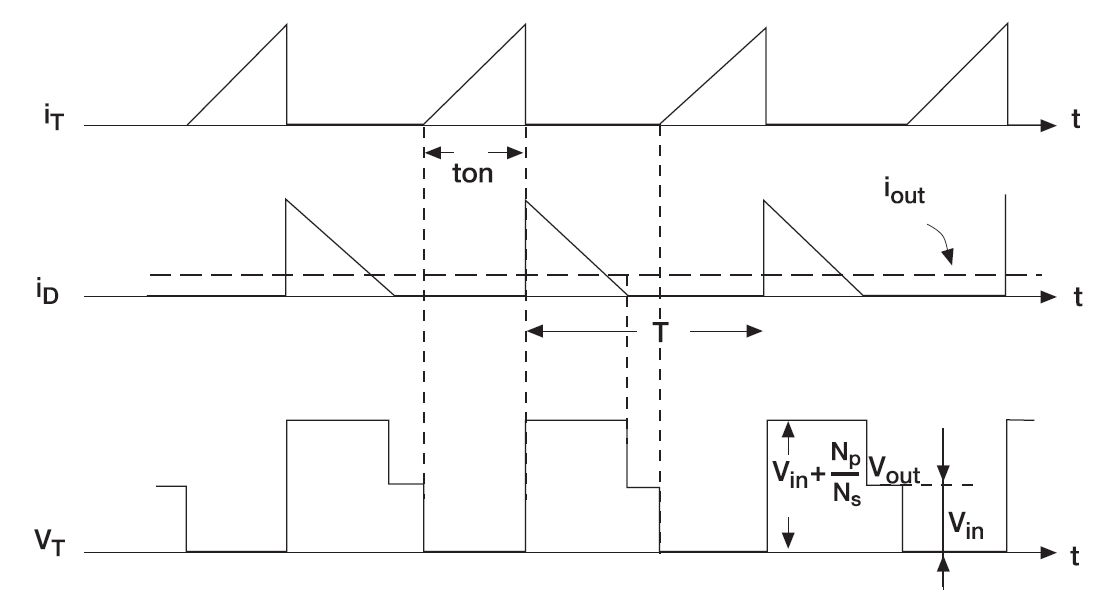
\includegraphics[max width=0.7\linewidth]{/tex/1iteration/billeder/DCM_transformer_current.PNG}
	\caption{DCM transformator strømme
		\cite{SMPS-topologies}}
	\label{fig:DCM_transformer_current}
\end{figure}

Overføringsfunktionen for flyback converteren i DCM er\cite{SMPS-topologies}:
\begin{equation} \label{flyback_converter_DCM_overforinsfunktion}
V_{out} = \frac{N_S}{N_P} \cdot \frac{D}{1-D} \cdot V_{in}
\end{equation}



\section{Ideel transformator}
Der vælges at arbejde videre med en flyback converteren, pga. komplikationerne ifm. switchingen af MOSFET'en ved buck converteren.
Der regnes strømme i transformatoren for både CCM og DCM, for derefter, at vurdere forskellene mellem de to metoder.

Der tages udgangspunkt i en converter der, ved en input spænding på $26V-50V$, skal kunne opretholde en udgang på $21V$ og $2.5A$. Derudover antages det at transformatoren har et omsætningsforhold på 1.

\subsection{CCM}
Først beregnes den maksimale og minimale duty-cycle:
\begin{equation} \label{D_maks_CCM}
D_{maks} = \frac{V_{out}}{V_{inmin} + V_{out}} = 0.447
\end{equation}
\begin{equation} \label{D_min_CCM}
D_{min} = \frac{V_{out}}{V_{inmaks} + V_{out}} = 0.174
\end{equation}

\noindent Nu kan de maksimale ripple-, peak- og RMS-strømme i transformatoren estimeres. 
\begin{equation} \label{I_ripple_CCM}
I_{ripple} = 0.6 \cdot \frac{V_{out} \cdot I_{out}}{V_{inmaks} \cdot   D_{min}} = 2.13A
\end{equation}
\begin{equation} \label{I_pk_CCM}
I_{pk} = \frac{V_{out} \cdot I_{out}}{V_{inmin} \cdot D_{maks}} + \frac{I_{ripple}}{2} = 5.58A
\end{equation}
\begin{equation} \label{I_pk_avg_CCM}
I_{pkavg} = \frac{I_{out}}{1-D_{maks}} = 4.52A
\end{equation}

\noindent Nu beregnes RMS-strømmene i både primær- og sekundærviklingerne. 
\begin{equation} \label{I_p_RMS_CCM}
I_{RMSp} = \sqrt{D_{maks} \cdot (I_{pkavg})^2} = 3.02A
\end{equation}
\begin{equation} \label{I_s_RMS_CCM}
I_{RMSs} = \sqrt{(1-D_{maks}) \cdot (I_{pkavg})^2} = 3.36A
\end{equation}

Induktansen i primærviklingen beregnes ud fra den ønskede ripplestrøm, samt switch-frekvensen. Som udgangspunkt vælges den til $100kHz$. Fordi omsætningsforholdet i transformatoren er lig 1, betyder det at $L_p = L_s$.
\begin{equation} \label{L_CCM}
L = \frac{V_{inmin} \cdot D_{min}}{I_{ripple} \cdot f_s} = 69.43\micro H
\end{equation}

\subsection{DCM}
Nu foretages strøm beregninger for en flyback converter i DCM.
Da overføringsfunktionen for CCM og DCM er den samme, betyder det både den maksimale og minimale duty-cycle er ens ved de to.
Derfor startes der med at regne peak-strømmen. Strømmen regnes ved det der kaldes boundary, som er det punkt hvor transformatoren lige præcis når at aflade i en switch-periode.
\begin{equation} \label{DCM_peak_current}
I_{pk} = I_o \cdot \frac{2}{1-D_{maks}} = 9.04A
\end{equation}

Da transformatoren når at aflade ved DCM er ripple-strømmen lig peak-strømmen:
\begin{equation} \label{DCM_ripple_current}
I_{ripple} = I_{pk} = 9.04A
\end{equation}

Induktansen i primærviklingen beregnes igen ud fra ligning~\ref{L_CCM}. Da peak-strømmen, og dermed også ripple-strømmen er regnet ved boundary, betyder det at der regnes en maksimal induktans, for hvor converteren stadig operer i DCM.
\begin{equation} \label{L_DCM}
L = \frac{V_{inmin} \cdot D_{min}}{I_{ripple} \cdot f_s} = 12.85\micro H
\end{equation}

Da induktansen er en maksimal værdi, skal man ligge med en hvis margin til denne, for at sikre, at converteren operer i DCM. Hvis induktansen i viklingerne mindskes, vil man opnå en større peak-strøm i transformatoren. Med en ripple-strøm på minimum $9.04A$, vurderes det at effekttabene ved at operere i DCM, vil blive for store. Derfor vil der fremadrettet arbejdes videre med en flyback converter i CCM.


\section{Udgangskondensator}
I en flyback converter bruges udgangskondensatoren primært til at mindske ripplespændingen på load'en. Formlen for at beregne minimumskapaciteten er
\begin{equation} \label{udgangskondensator}
C_{out} \geqslant \frac{I_{out} \cdot D_{maks}}{V_{ripple} \cdot f_s} \geqslant 223.4 \micro F
\end{equation}

\section{Simulering}
Med udgangspunkt i figur~\ref{fig:flyback_ideal} opsættes en ideel flyback converter i p-spice. Dette er gjort på figur~\ref{fig:ideal_flyback_diagram}. Converteren er sat op med en ideel transformatorkobling, et ideelt switching element, samt en ideel diode, for at få et indblik i flyback converterens virkemåde. 


\begin{figure}[H]
	\center
	\includegraphics[max width=0.7\linewidth]{/tex/1iteration/billeder/flyback_ideal_diagram.PNG}
	\caption{Ideelt flyback kredsløb}
	\label{fig:ideal_flyback_diagram}
\end{figure}

Der er to scenarier der er relevante at kigge på, ved en indgangsspænding på $26V$, samt ved en indgangsspænding på $50V$. Først kigges der på udgangen af converteren, for at kontrollere udgangsstrømmen og -spændingen. På figur~\ref{fig:26V_ideal_output} ses både outputstrømmen (rød) og -spændingen (grøn), med en inputspænding på 26V. Her ses det at spændingen ligger sig omkring $21V$ og strømmen ligger sig omkring $2.5A$, hvilket var kravet til converteren. Derudover aflæses ripplespændingen til ca. $50mV$, hvilket er overholder kravet for ripplespændingen. 

\begin{figure}[H]
	\center
	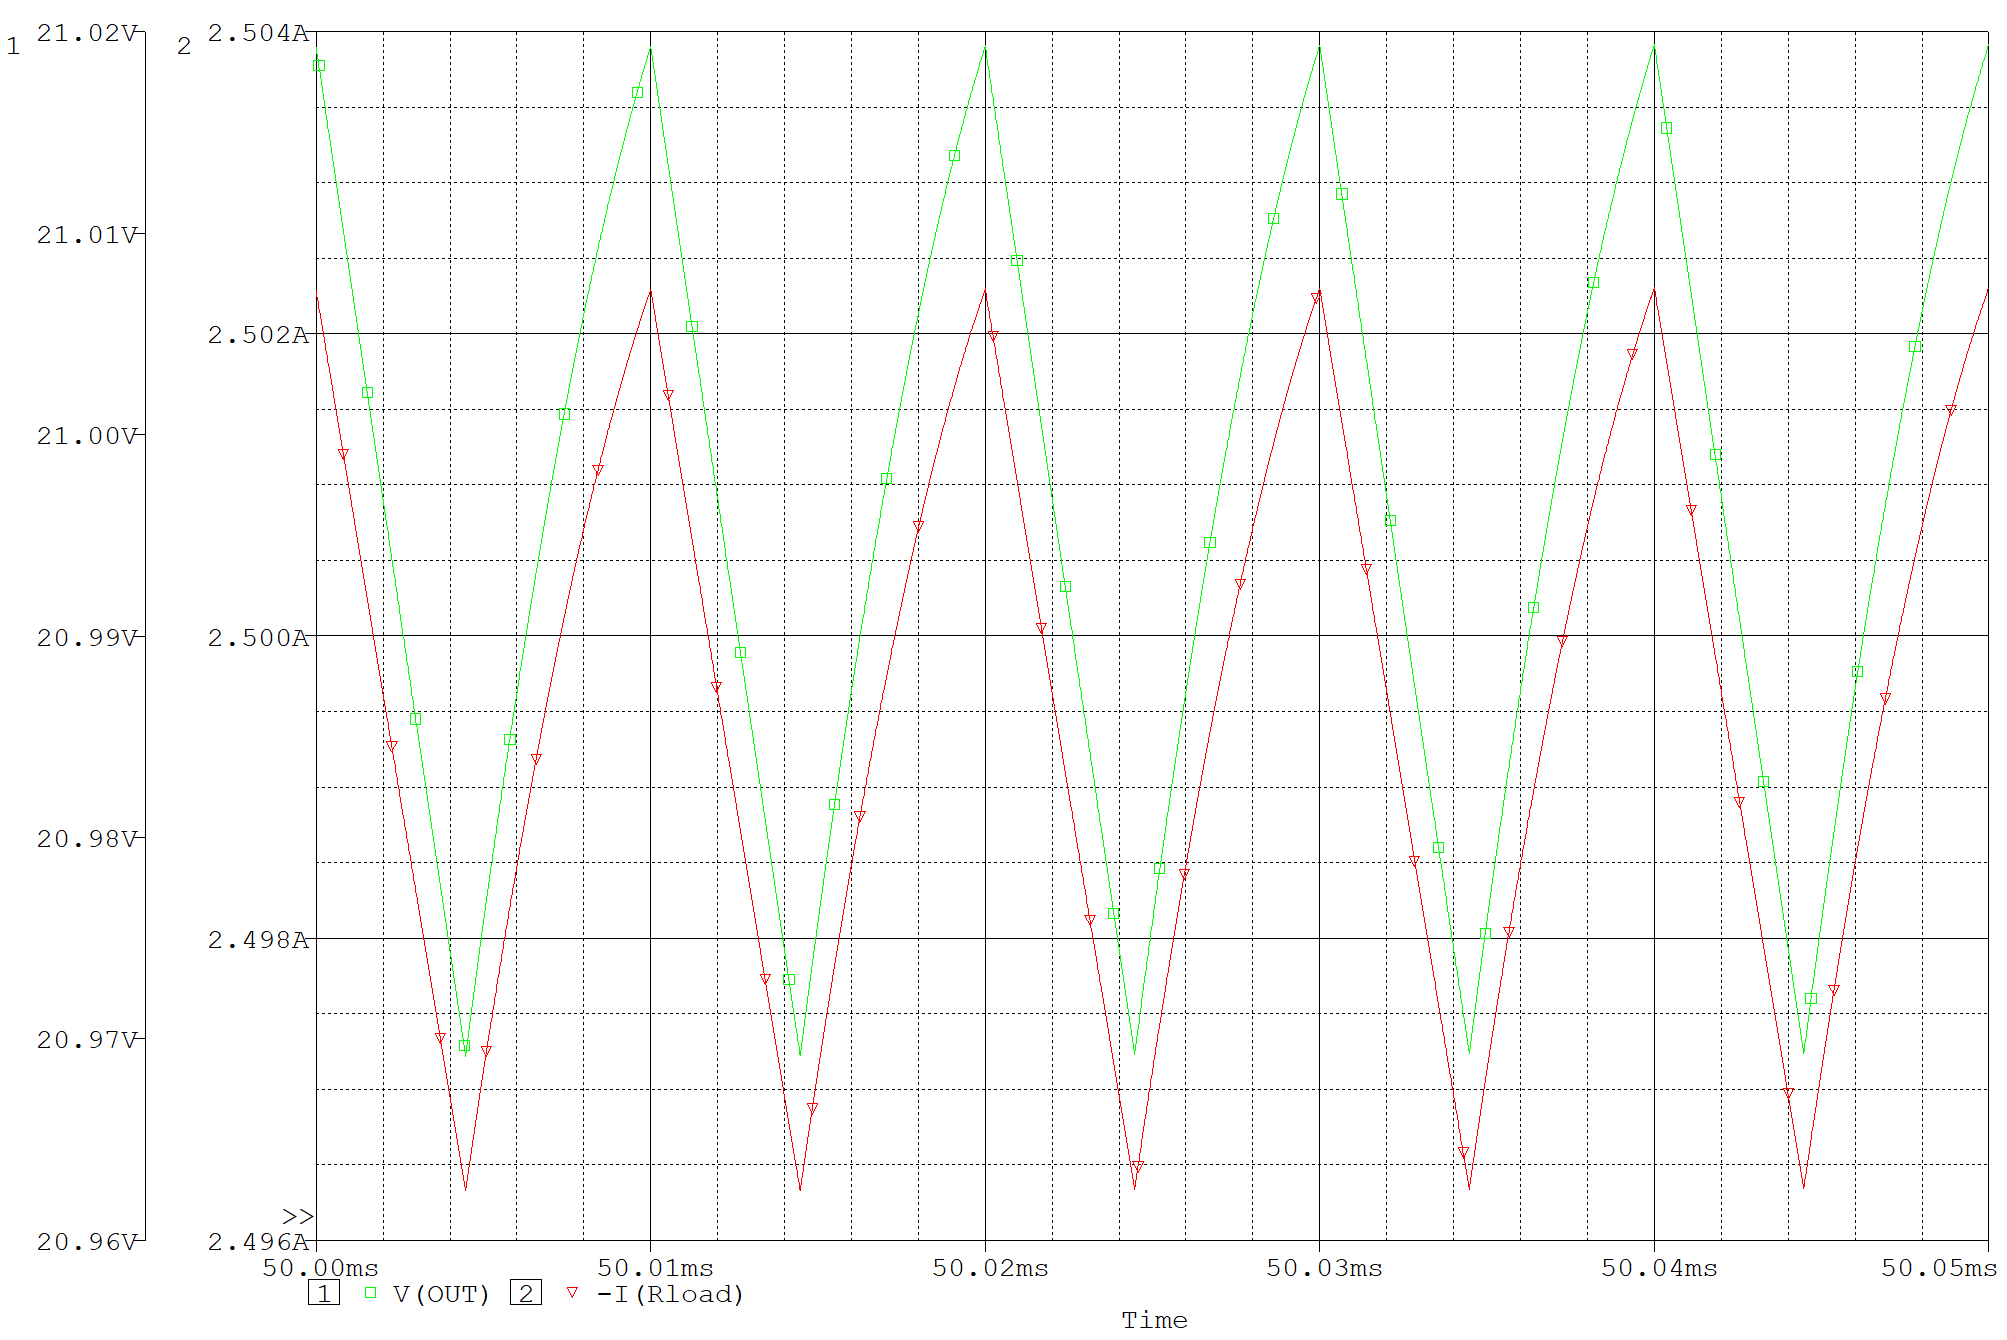
\includegraphics[max width=0.7\linewidth]{/tex/1iteration/billeder/26V_output.PNG}
	\caption{Converter output - ved 26V input}
	\label{fig:26V_ideal_output}
\end{figure}

\noindent På figur~\ref{fig:50V_ideal_output} ses det samme billede, ved $50V$ inputspænding. Da converterens duty-cycle er faldet, falder ripple-spændingen også. Den aflæses til ca. $33mV$. 


\begin{figure}[H]
	\center
	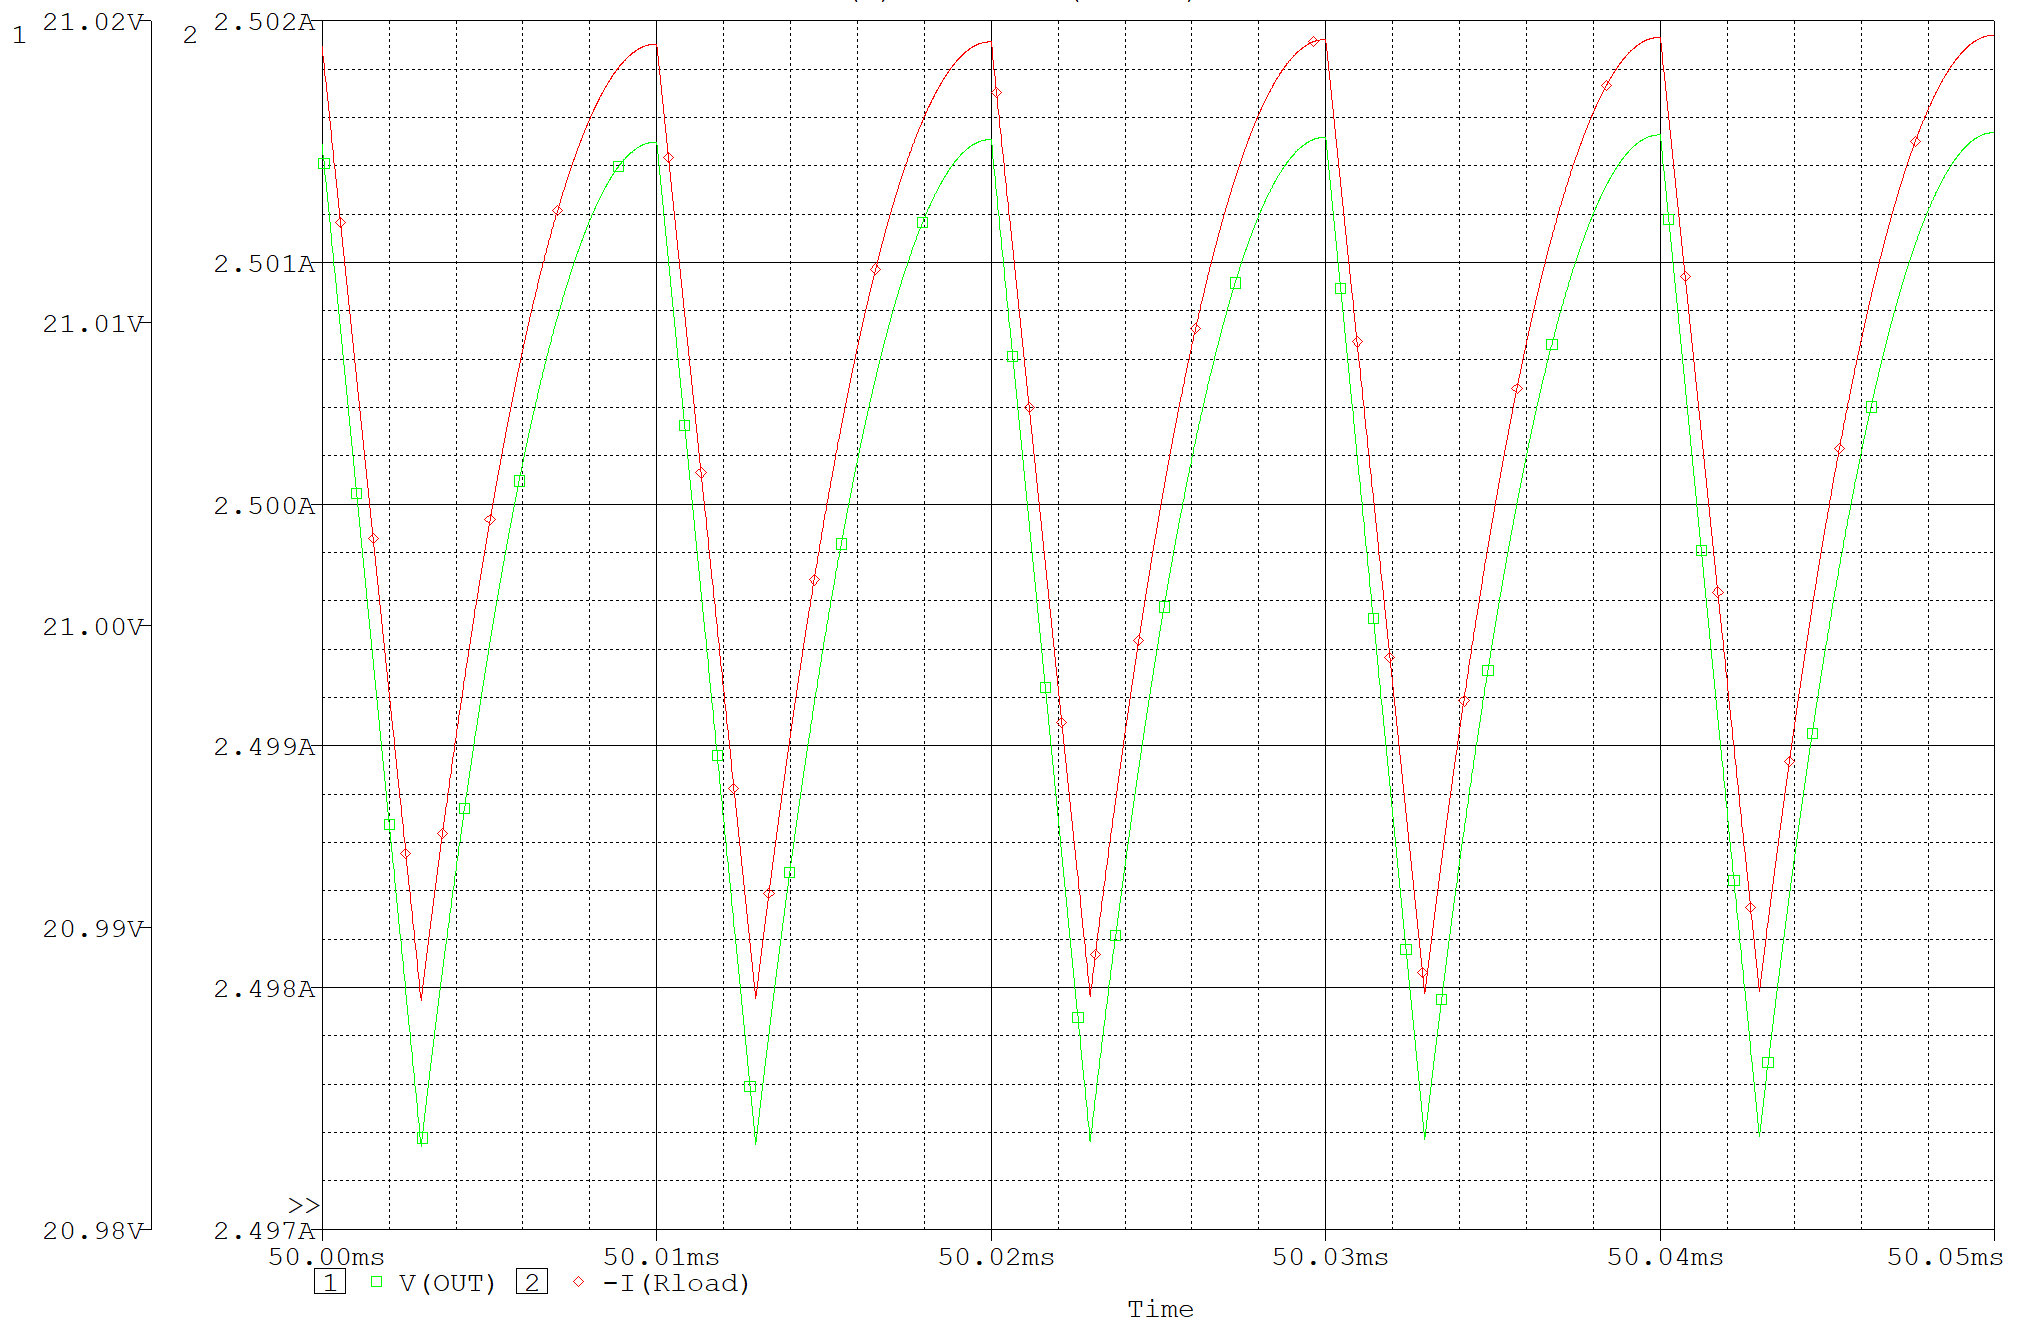
\includegraphics[max width=0.7\linewidth]{/tex/1iteration/billeder/50V_output.PNG}
	\caption{Converter output - ved 50V input}
	\label{fig:50V_ideal_output}
\end{figure}

\noindent I tabel~\ref{tab:result_ideal_converter} ses resultaterne for analyse(A) og simulering(S), af den ideelle converter. Ripple- og peak-strømmene er aflæst ud fra figur~\ref{fig:26V_transformer_current} og \ref{fig:50V_transformer_current}. RMS-strømmene findes ved, at bruge RMS-funktionen i p-spice. Derudover kan det konstateres at converteren operer i CCM, da transformatorstrømmen ikke når at aflade helt. Se figur~\ref{fig:CCM_transformer_current}. 

\begin{table}[H] 			
	\centering
	\begin{tabularx}{\textwidth}{|X|c|c|c|c|c|c|c|c|}
		\hline
		\textbf{Indgangs-spænding} & \multicolumn{2}{|X|}{\textbf{Ripple-strøm}} & \multicolumn{2}{|X|}{\textbf{Peak-strøm}} & \multicolumn{2}{|X|}{\textbf{RMS-strøm i primær}} & \multicolumn{2}{|X|}{\textbf{RMS-strøm i sekundær}} \\ \hline
		& A & S & A & S & A & S & A & S \\ \hline
		$26V$ & $1.67A$ & $1.66A$ & $5.36A$ & $5.35A$ & $3.02A$ & $3.08A$ & $3.36A$ & $3.33A$ \\ \hline 
		$50V$ & $2.13A$ & $2.11A$ & $4.62A$ & $4.61A$ & $1.93A$ & $1.98A$ & $2.98A$ & $3.01A$ \\ \hline
	\end{tabularx}
	\caption{Resultater for analyse og simulering af ideel flyback converter}
	\label{tab:result_ideal_converter}
\end{table}

\begin{figure}[H]
	\center
	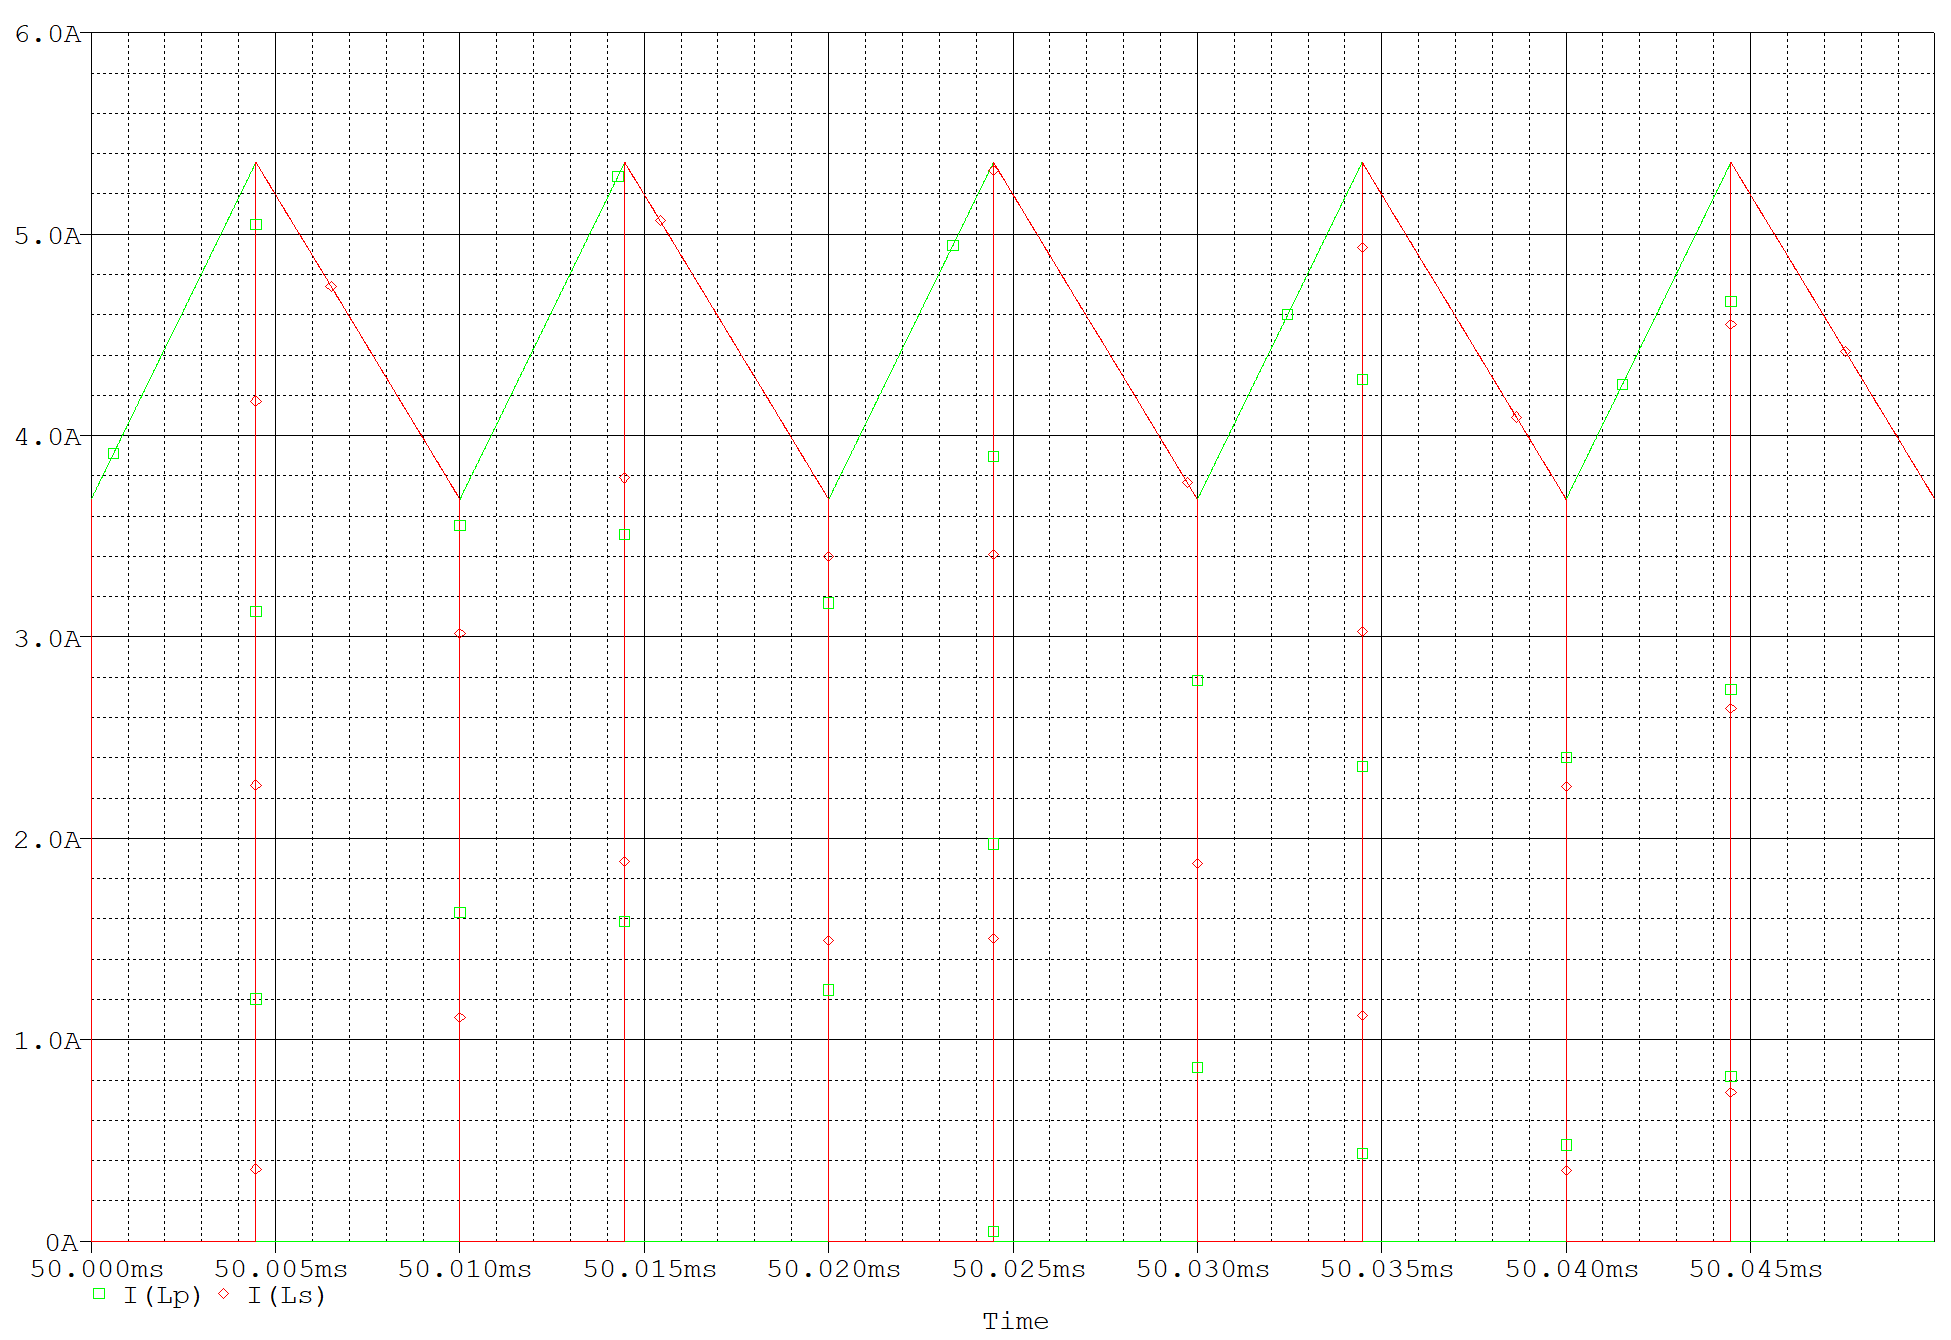
\includegraphics[max width=0.7\linewidth]{/tex/1iteration/billeder/26V_transformer_current.PNG}
	\caption{Transformator strømme - ved 26V input}
	\label{fig:26V_transformer_current}
\end{figure}

\begin{figure}[H]
	\center
	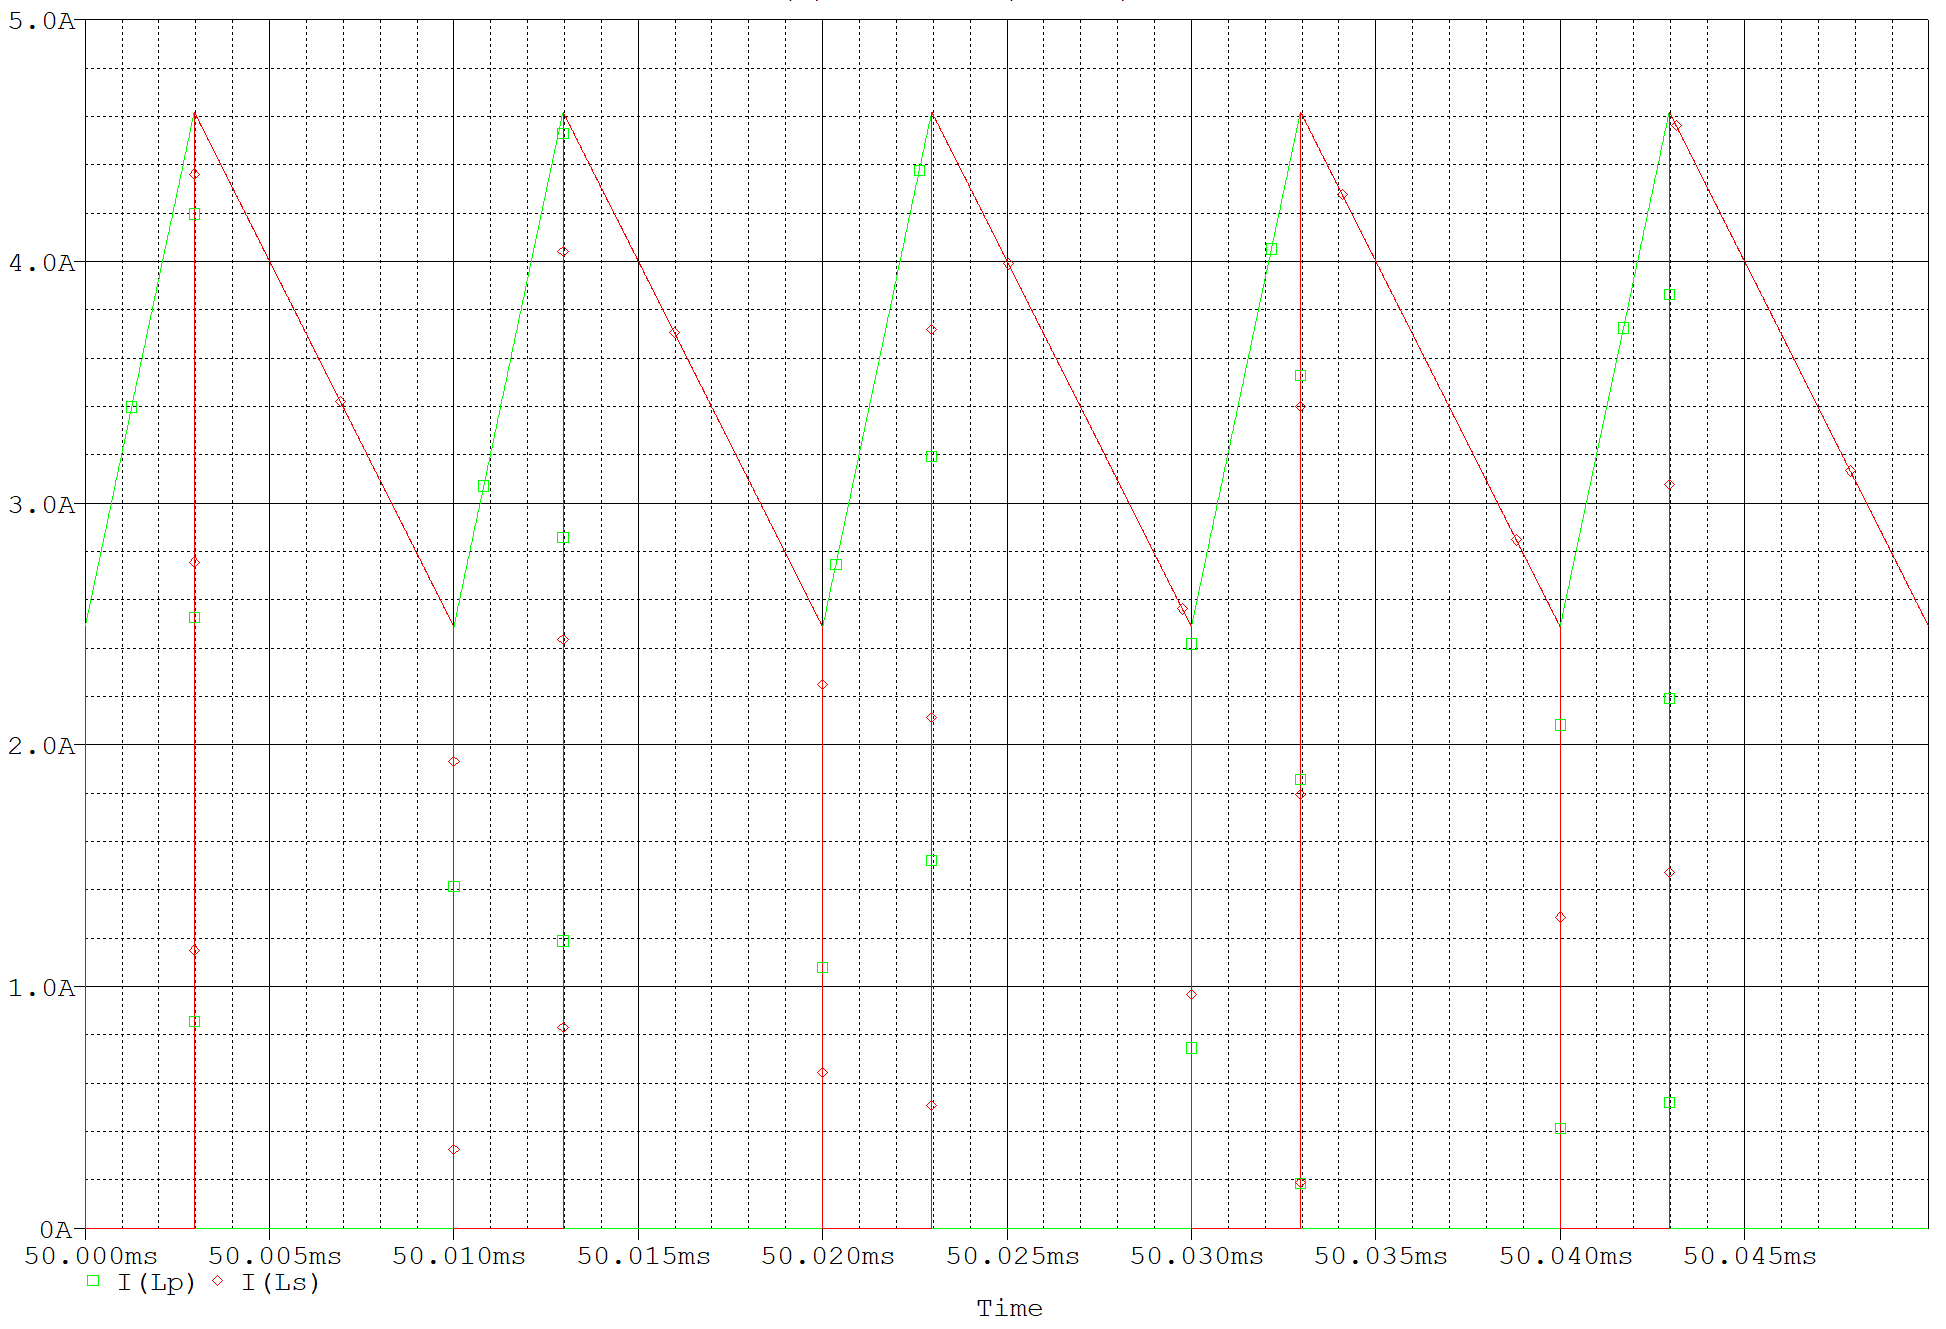
\includegraphics[max width=0.7\linewidth]{/tex/1iteration/billeder/50V_transformer_current.PNG}
	\caption{Transformator strømme - ved 50V input}
	\label{fig:50V_transformer_current}
\end{figure}





\chapter{Anden Iteration}
I dette afsnit beskrives 2. iteration af design- og implementeringsfasen. Den indebærer design og vikling af transformator samt valg af resterende komponenter i kredsløbet. Yderligere realiseres og testes hele kredsløbet for første gang i 2. iteration.

\section{Transformator}
Transformeren fungerer anderledes ved en flyback end ved de fleste andre SMPS, hvor der løber en strøm i de primære og sekundære viklinger på samme tid. Det er ikke tilfældet ved en flyback konstruktion. Her løber strømmen kun i en vikling af gangen. Når MOSFET’en er ON, vil strømmen igennem den primære vikling rampe op i forhold til indgangsspændingen og induktansen i viklingen. Pga. dioden og polariteten af den sekundære vikling, vil der på dette tidspunkt, ikke løbe en strøm i viklingen. Når transistoren går OFF falder strømmen i den primære vikling til 0, som får spændingerne over viklingerne til at skifte polaritet. Med en modsat polaritet på sekundærsiden, kan der nu løbe en strøm gennem dioden. 


Normalt kan energien fra den primære vikling transformeres direkte over i den sekundære vikling, da der løber en strøm på samme tid. Da det ikke er tilfældet ved flyback, kræver konstruktionen, at transformatoren kan opbevare energien fra den primære vikling, indtil det kan transformeres over i den sekundære vikling. Det gør, at der i transformatoren er behov for et luftgab i kernen, for transformatoren ikke skal gå i mætning. Luftgabet vil generere en større magnetisk modstand i kernen. Når den magnetiske modstand stiger, vil det blive muligt at opbevare en større energi i kernen, uden den går i mætning. 


Det er flux-ændringen i kernen, der sørger for, at der induceres en spænding over i den sekundære vikling. Det vil sige, at der er behov for at fluxen i kernen ændrer sig forholdsvis lineært, hvilket sker når der ligger en konstant spænding over viklingen. Kernen siges at have nået mætning, når en ændring i H-feltet ikke længere ændrer lineært på fluxen. 


For at sikre transformatoren ikke går i mætning, bruges hysteresekurven (ses på figur~\ref{fig: Hysteresekurve}) som plotter H-feltet på x-aksen og B-feltet op ad y-aksen. Her skal det undgås at transformatoren kommer til at blive vandret i top og/eller bund, da det er her, at transformatoren går i mætning. Yderligere fås et overblik over selve transformatortabet ud fra samme kurve. Det areal, som kurven indeholder, er nemlig tabet i transformatoren per switch-periode. Det betyder ligeledes, at kernetabet bliver større, jo højere switch frekvens der benyttes. 

\begin{figure}[H]
	\center
	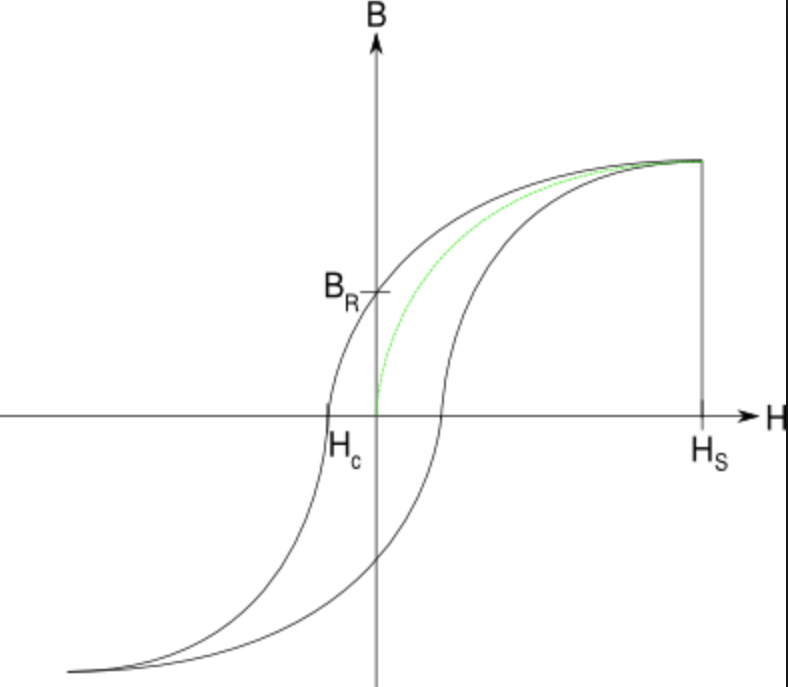
\includegraphics[max width=0.7\linewidth]{/tex/2iteration/billeder/Hysteresekurve.png}
	\caption{Hysteresekurve}
	\label{fig: Hysteresekurve}
\end{figure}


Effektiviteten i transformatoren betegens, ved koblingen mellem primær- og sekundærviklingerne. Den manglende kobling skyldes, det ikke er hele magnetfeltet der vil blive induceret i kernen. Det vil i stedet blive spredt ud i luften, og bliver derfor betegnet som spredningsselvinduktionen i transformatoren. Spredningsselvinduktionen er unik for transformatoren, og afhænger meget af hvordan den vikles. 


\subsection{Design}
Først og fremmest skal ripplestrømmen, som der løber i transformatoren bestemmes. Dette er gjort i 1. iteration, hvor ripplestrømmen blev bestemt til $I_{ripple} = 2.13A$.

Dernæst skal den nødvendige induktion det kræver for, at transformatoren kan rampe op til den nødvendige strøm, inden for duty-cyclen udregnes. Dette er også gjort i 1. iteration hvor $L=69.43\micro H$.

Som beskrevet tidligere skal kernen kunne opbevare den energi som kommer fra primær viklingen, når transistoren er on, for at undgå mætning. Mængden af energi i primærviklingen udregnes ved:
\begin{equation} \label{Primary_energy}
E = \frac{1} {2} \cdot L \cdot {I_{pk}}^2 = 1.083\milli J
\end{equation}

For at beregne den tilladelige mængde energi der kan oplagres i transformatoren, skal kernen og kernematerialet kendes. Valget er her faldet på en RM8 kerne\cite{RM8} og materialet 3f3\cite{3f3}. RM8 kernens mål gør, at den lige akkurat kan være på printet højdemæssigt. Derudover har Terma tidligere brugt RM8 kerner med 3f3 og har nogle mere præcise mål på $A_L$ og luftgab, end det oplyste i datasheets’ne. Det er essentielt for præcisionen af en fremtidig simulering, at det korrekte luftgab bruges, for at kunne sammenholde simulering og realisering.


Den effektive volumen, $V_e$, aflæses for RM8. På databladet for 3f3 aflæses et maks peak af B-feltet til lidt over $300\milli T$. Hvis der designes efter, at transformatoren vil operere med et højere B-felt, vil det risikeres at kernen går i mætning. Derfor vælges det, at designe med en $B_{maks}=250mT$, da det vil sikre en god margin til mætning. Yderligere findes permeabiliteten for 3f3 materialet uden luftgab. Med disse oplysninger vil transformatoren kunne opbevare følgende energi:
\begin{equation} \label{Energy_no_gap}
w_{kerne} = \frac{1} {2} \cdot \frac{1}{\micro_e} \cdot B^2 \cdot V_e = 53\pico J
\end{equation}

Det er tydeligt at den nødvendige energi på ingen måde kan opbevares i kernen. Da ferrit kan opbevare så lidt energi som det er tilfældet, kan det estimeres at al energien vil blive opbevaret i det luftgap, der designes. Derfor kan permeabiliteten ses som $\micro_0$ i den nye beregning. Den effektive volumen deles op i luftgab og $A_L$, så luftgabet kan isoleres. Med dette kan luftgabet beregnes: 
\begin{equation} \label{Airgap}
l_g = \frac{L \cdot {I_{pk}}^2 \cdot \micro_0}{B^2 \cdot A_0} = 690.98\micro m
\end{equation}

Med den ripplestrøm der i første omgang er benyttet, skal der bruges et luftgab på ca. $691\micro m$. Den nærmeste luftgab værdi for 3f3 ligger på $488\micro m$ hvilket giver en $A_L$ på $160\nano H$. (Dette er ikke databladets værdi, men en værdi der er blevet givet fra Terma, som har testet databladets værdier til ikke at være korrekte.) Med det udregnede luftgab, beregnes den tilhørende induktion i transformatoren. 
\begin{equation}
L_1 = \frac{l_g \cdot B^2 \cdot A_0}{{I_{pk}}^2 \cdot \micro_0} = 49.035\micro H
\end{equation}

\noindent Med kendt $A_L$ og induktion kan vindingstallet beregnes. Da der i 2. iteration bruges en 1:1 transformator er dette både for primær- og sekundærvikling:
\begin{equation} \label{N}
N = \sqrt{\frac{L_1}{A_L}} = 17.5 \approx 18
\end{equation}
Det passer fint med 18 viklinger på hver side, hvor induktansen igen bliver lidt anderledes når vindingstallet rundes op. 
\begin{equation} \label{L1}
L_2 = N^2 \cdot A_L = 51.84 \micro H
\end{equation}
Med fastlagt induktans kan ny ripple- og peak strøm beregnes.
\begin{equation}
I_{ripple} = \frac{V_{inmin} \cdot D_{max}}{L_2 \cdot f_s} = 2.24A
\end{equation}
\begin{equation}
I_{pk} = \frac{V_{out} \cdot I_{out}}{V_{inmin} \cdot D_{maks}} + \frac{I_{ripple}}{2} = 5.64A
\end{equation}

\subsection{Simulering} \label{Simkernetab}
I Pspice er kernen og materialet simuleret, hvor resten af kredsløbet har været med ideelle komponenter, for at kontrollere strømme og B-H kurve. Her ses den pspice-model af kernematerialet som bruges:
\begin{figure}[H]
	\center
	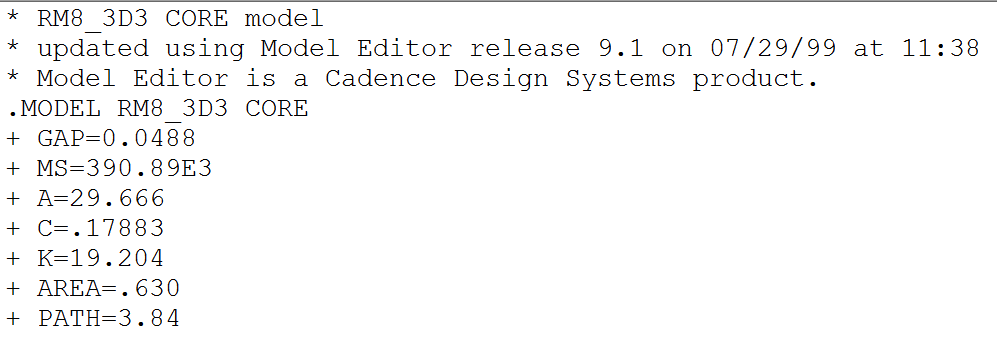
\includegraphics[max width=0.7\linewidth]{/tex/2iteration/billeder/Kernemodel.png}
	\caption{Kernemodel for RM8 3f3}
	\label{fig: Kernemodel}
\end{figure}


Kernemodellen for en 3f3 kerne er indsat, hvor det udregnede luftgab også er indtastet. Derudover er der 18 vindinger på primær og sekundærspole. Ellers ingen ændringer i forhold til den rent ideele simulering. Først ses simuleringen af strømmene i transformatoren på primær og sekundær side.
\begin{figure}[H]
	\center
	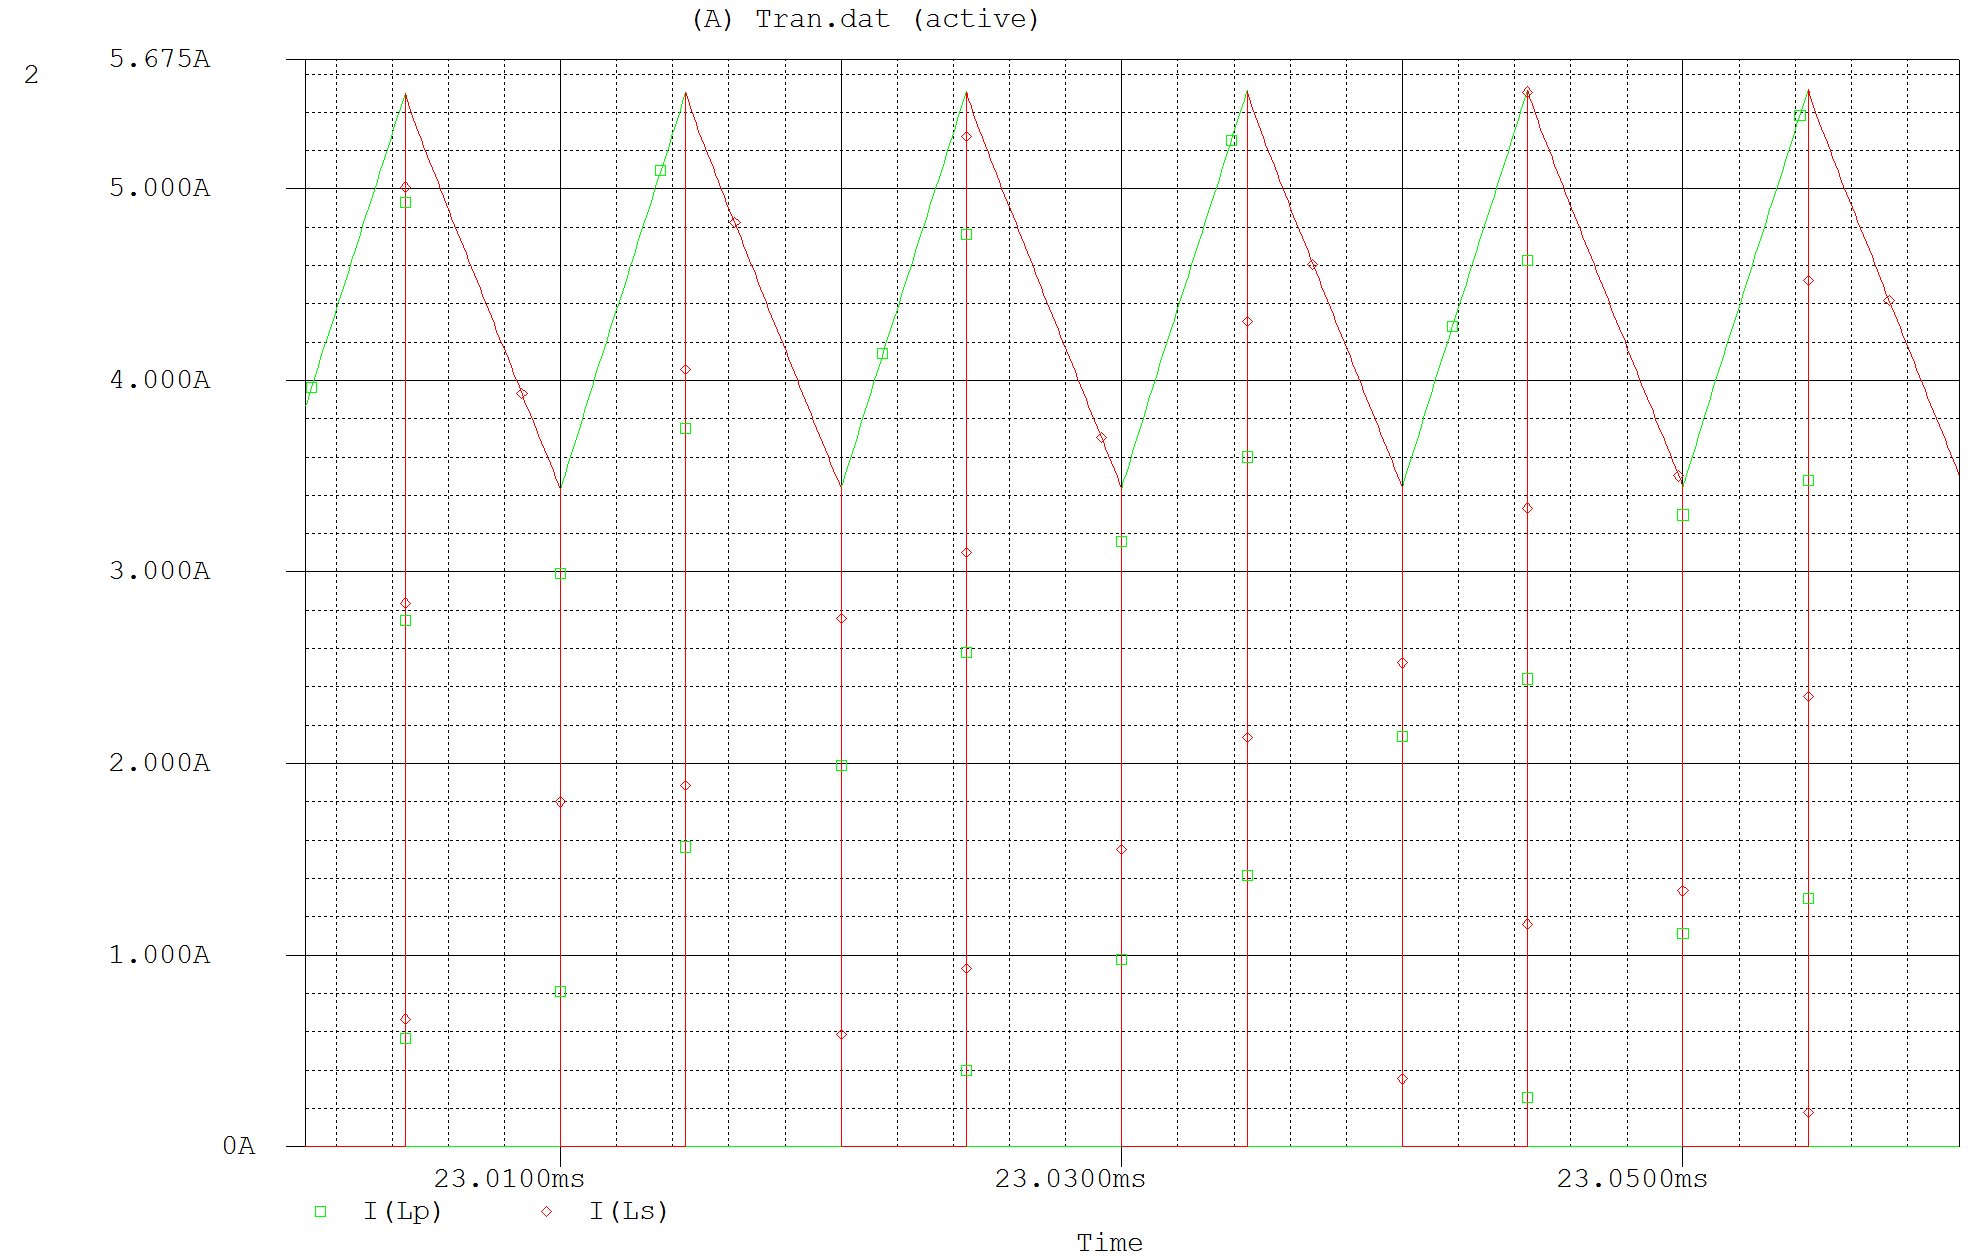
\includegraphics[max width=0.7\linewidth]{/tex/2iteration/billeder/Strom_pri_sek.png}
	\caption{Strøm i primær- og sekundærvikling}
	\label{fig: prisek_strom}
\end{figure}
Det ses tydeligt, at der som ventes køres i CCM, da ripplestrømmene ikke når ned til 0. Ripple- og peak strøm er, som det ses, ens for primær og sekundær, og aflæses til hhv. $2.1A$ og $5.5A$. Det passer fint med det udregnede på $2.24A$ og $5.64A$.
På figur~\ref{fig: RMS_trans} ses RMS strømmene:
\begin{figure}[H]
	\center
	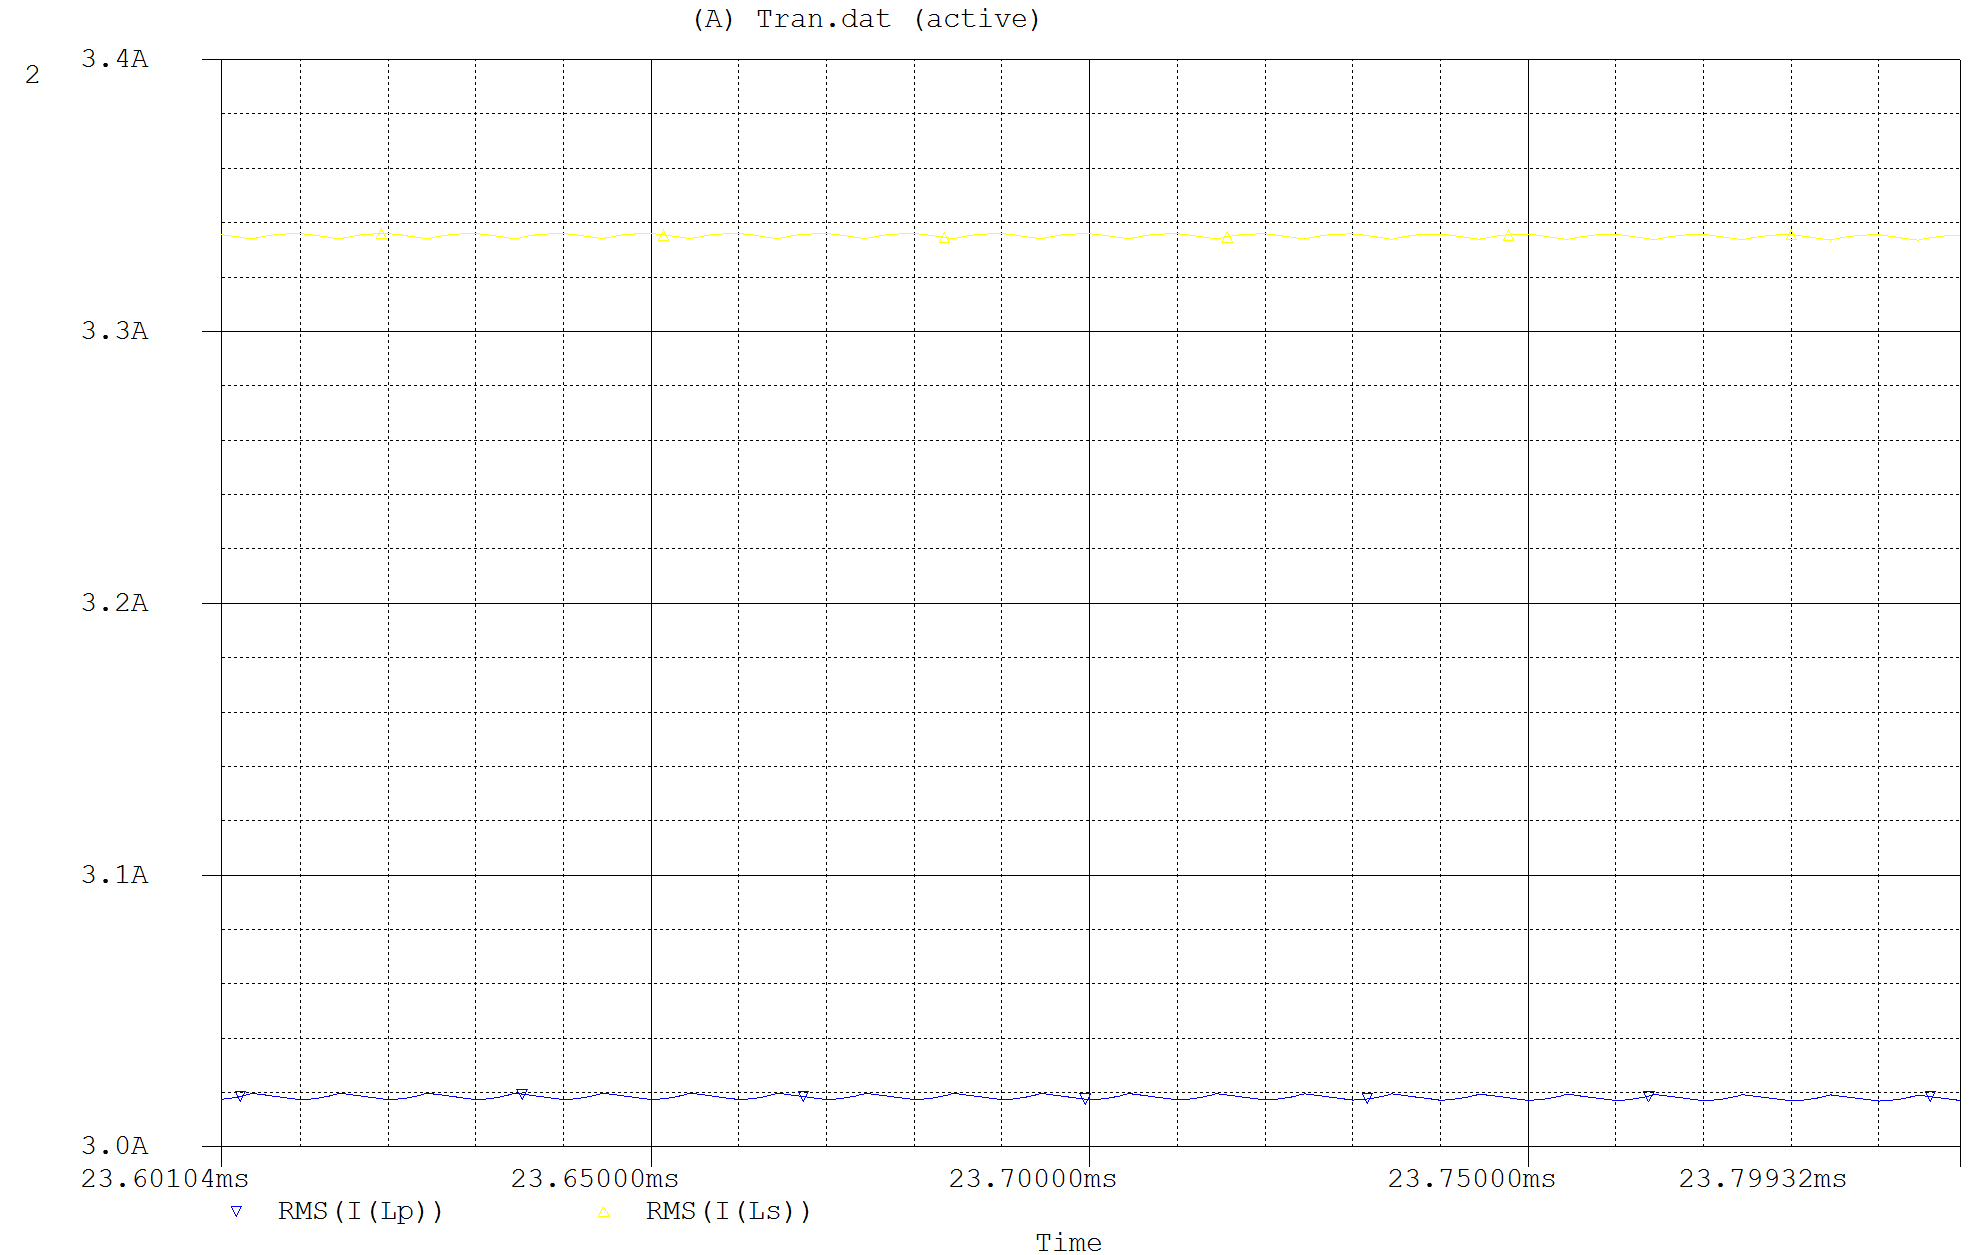
\includegraphics[max width=0.7\linewidth]{/tex/2iteration/billeder/RMS_transformator.png}
	\caption{RMS strømme i transformator (blå=primær og gul=sekundær)}
	\label{fig: RMS_trans}
\end{figure}

Her aflæses den RMS-strømmen i primærviklingen til $3.01A$ og i sekundærviklingen til $3.33A$, hvilket igen stemmer godt overens med det beregnede på $3.02A$ og $3.36A$.


\noindent Herefter kigges på hysteresekurven, og sikres at den ikke kommer langt over de $250\milli T$, som der er designet efter:
\begin{figure}[H]
	\center
	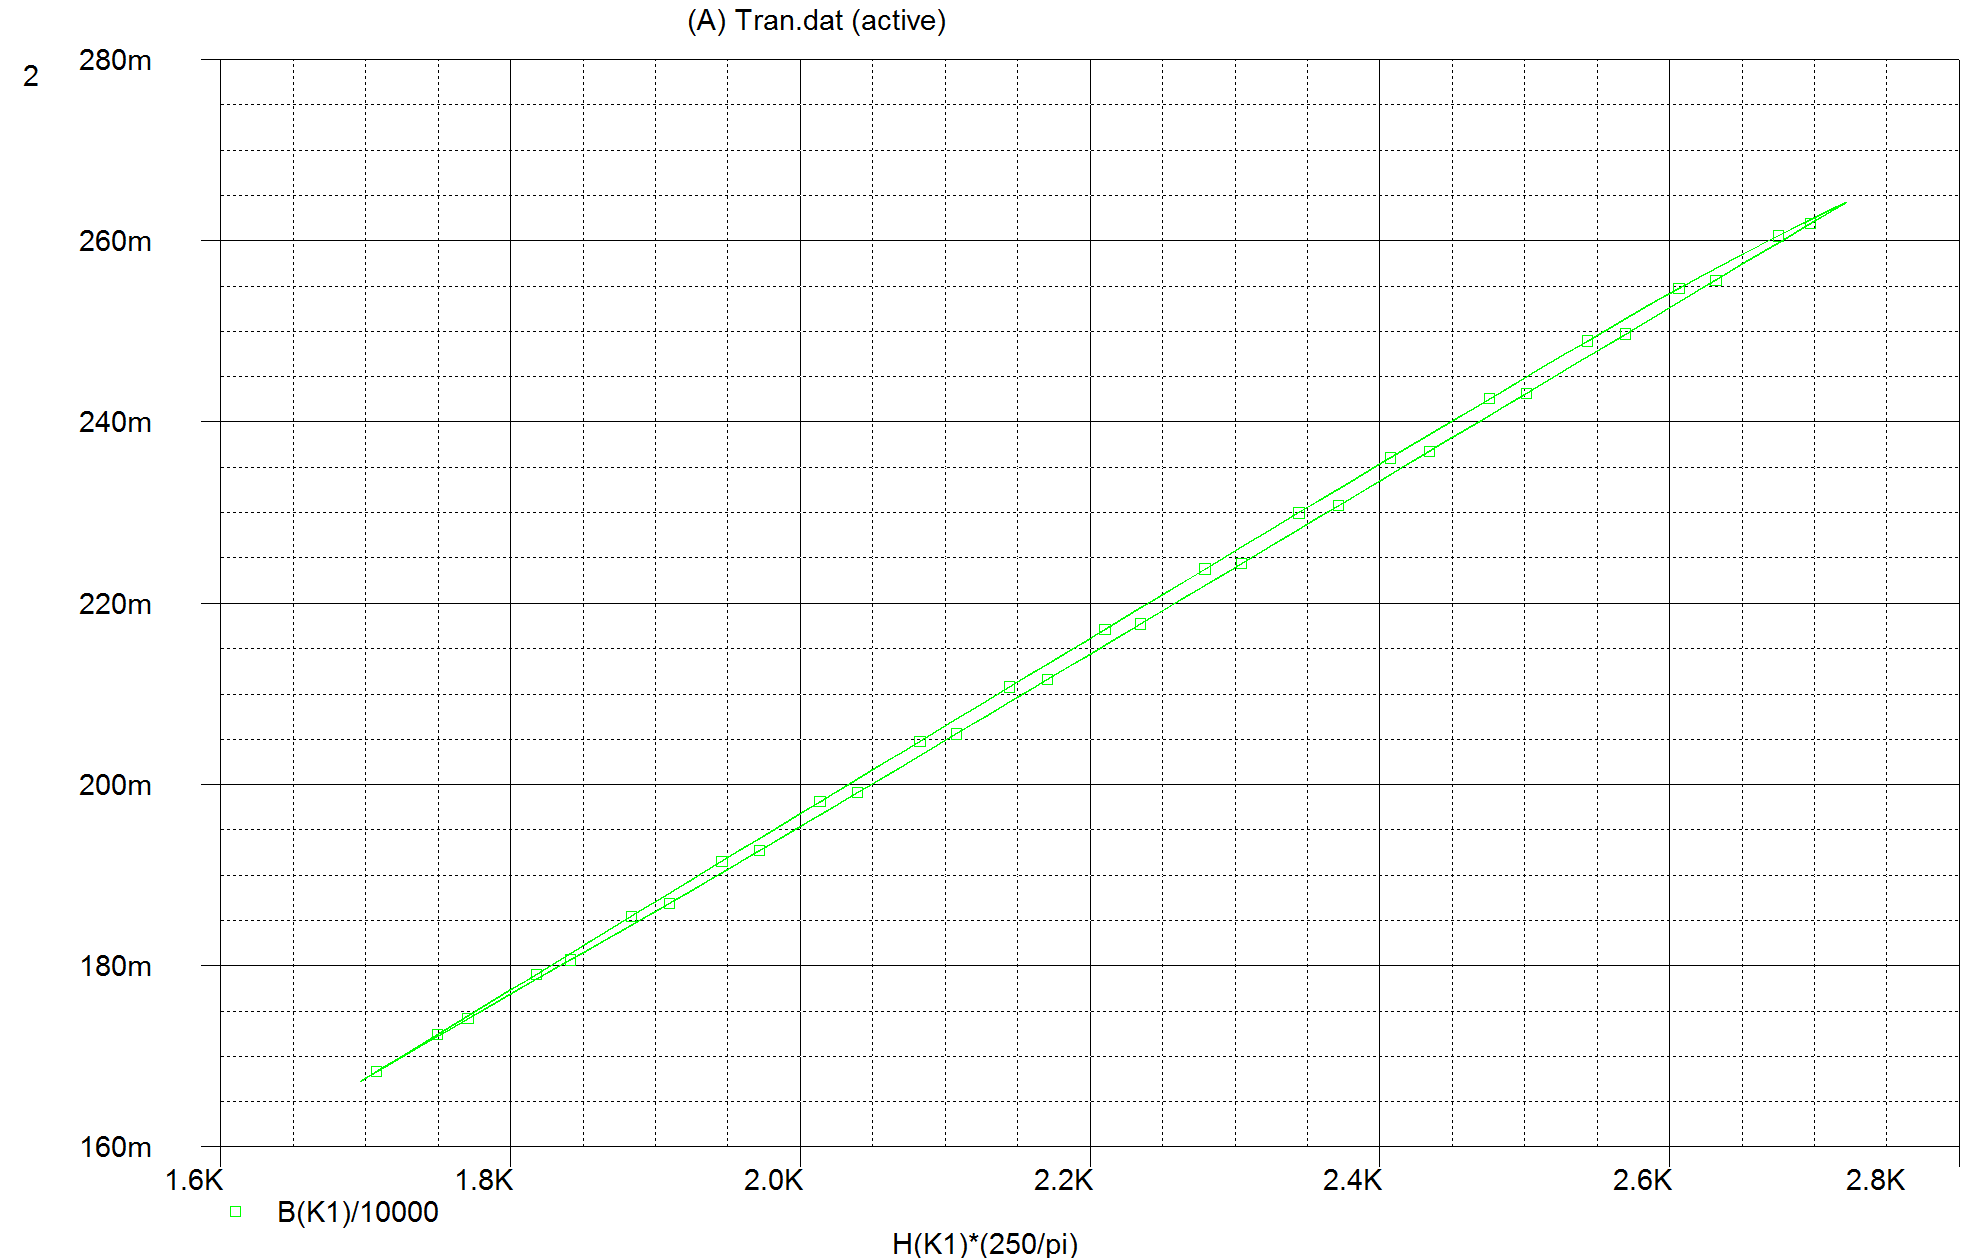
\includegraphics[max width=0.7\linewidth]{/tex/2iteration/billeder/Hysterese_trans.png}
	\caption{Hysteresekurve for transformatoren}
	\label{fig: Hysterese_trans}
\end{figure}
Peak fluxen ligger på ca. $265mT$ hvilket igen passer fint med det der er designet efter. Da induktansen er blevet rundet ned ved valg af luftgab, vil peak-fluxen stige en smule. Yderligere ville det kunne ses i toppen og bunden af kurven, hvis den gik i mætning, hvilket den ikke gør her.
Tabet i selve kernen er simuleret ved at tage effekten ved den primære vikling i forhold til den sekundære vikling. Tages der i pspice en average af dette fås nedenstående kurve:
\begin{figure}[H]
	\center
	\includegraphics[max width=0.7\linewidth]{/tex/2iteration/billeder/tabkerne.png}
	\caption{Simuleret kernetab i transformator}
	\label{fig: Kernetab}
\end{figure}
\noindent Tabet er simuleret til at ligge ved ca. $310\milli W$

\subsection{Vikling af transformator}
Det er vigtigt, at udnytte kernens mål fuldt ud når vindingerne vikles. Med RM8 kernen er der en bredde på $8.6\milli m$ og en højde på $3.475\milli m$. Ved 2. iteration forsøges de mål udnyttet bedst muligt.
Først udregnes den nødvendige diameter af tråden, når der skal ligge 18 vindinger per lag. 
\begin{equation} \label{d_trad}
d_{tråd} = \frac{8.6\milli m}{18} = 0.478\milli m
\end{equation}

Dette er dog den samlede diameter, altså inklusiv isolering. Der benyttes en isolering med grade 2, som giver en diameter på ledningen eksklusiv isolering på $0.425\milli m$\cite{wire-diameter}. Transformeren er 1:1, så både primær og sekundær vikles med 18 vindinger per lag. Et lag af hver giver en højde på $0.956\milli m$. Altså ikke i nærheden af de $3.475\milli m$ i højden. Derfor vikles 2 ekstra viklinger i parallel for både primær- og sekundærsiden og får dermed den tredobbelte højde. Der indsættes tape mellem hver af de parallelle viklinger, for at sikre viklingerne ikke rykker sig under viklingen af transformatoren. Det giver samlet en højde på $2.867\milli m$ eksklusiv tape. Det giver i alt 6 lag, 3 for primær og 3 for sekundær. Overblikket over viklingen kan ses på figur~\ref{fig: viklingsoverblik}:
\begin{figure}[H]
	\center
	\includegraphics[max width=0.7\linewidth]{/tex/2iteration/billeder/viklingsoverblik.png}
	\caption{Overblik over viklingsantal og tykkelse}
	\label{fig: viklingsoverblik}
\end{figure}

\noindent Tegnes bunden af transformatoren fås der et overblik over, hvordan viklingerne vikles. Det ses, at primær begynder og slutter i samme sidde af transformatoren, mens sekundær vikles fra den anden side. Ved at trække viklingerne ud på samme side, sikres det der altid vikles med hele vindinger.
\begin{figure}[H]
	\center
	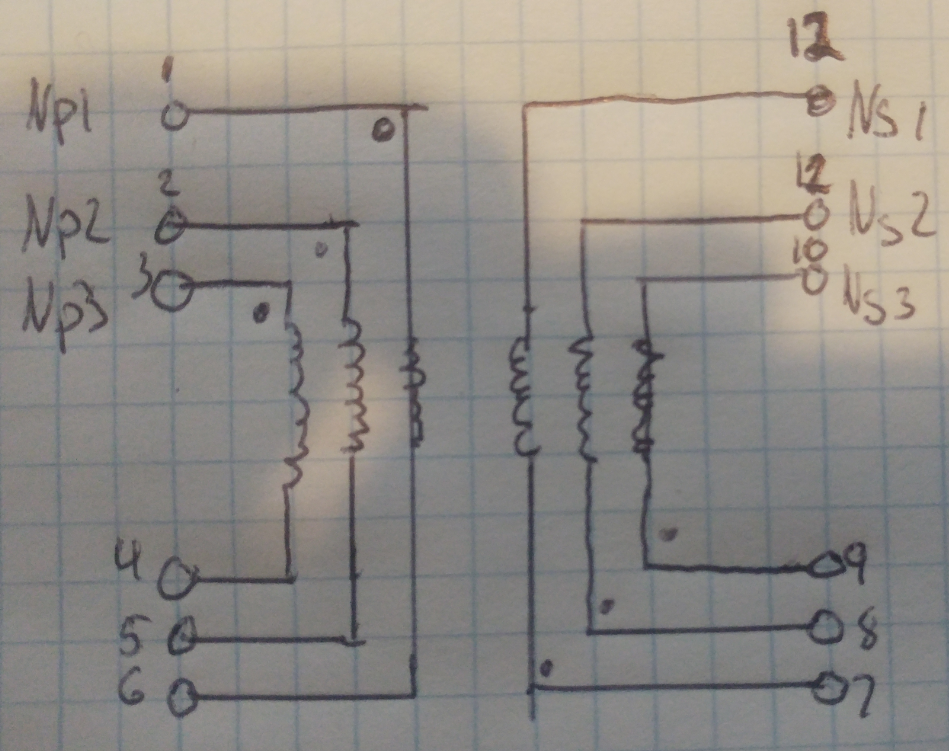
\includegraphics[max width=0.7\linewidth]{/tex/2iteration/billeder/Viklingsbegyndelse.png}
	\caption{Overblik over hvordan viklingerne vikles}
	\label{fig: viklingsbegyndelse}
\end{figure}

\noindent Sidste billede viser hvilken retning der vikles. Her vil primær og sekundær vikles modsatte vej af hinanden, for at få den modsatte polaritet som ønsket.
\begin{figure}[H]
	\center
	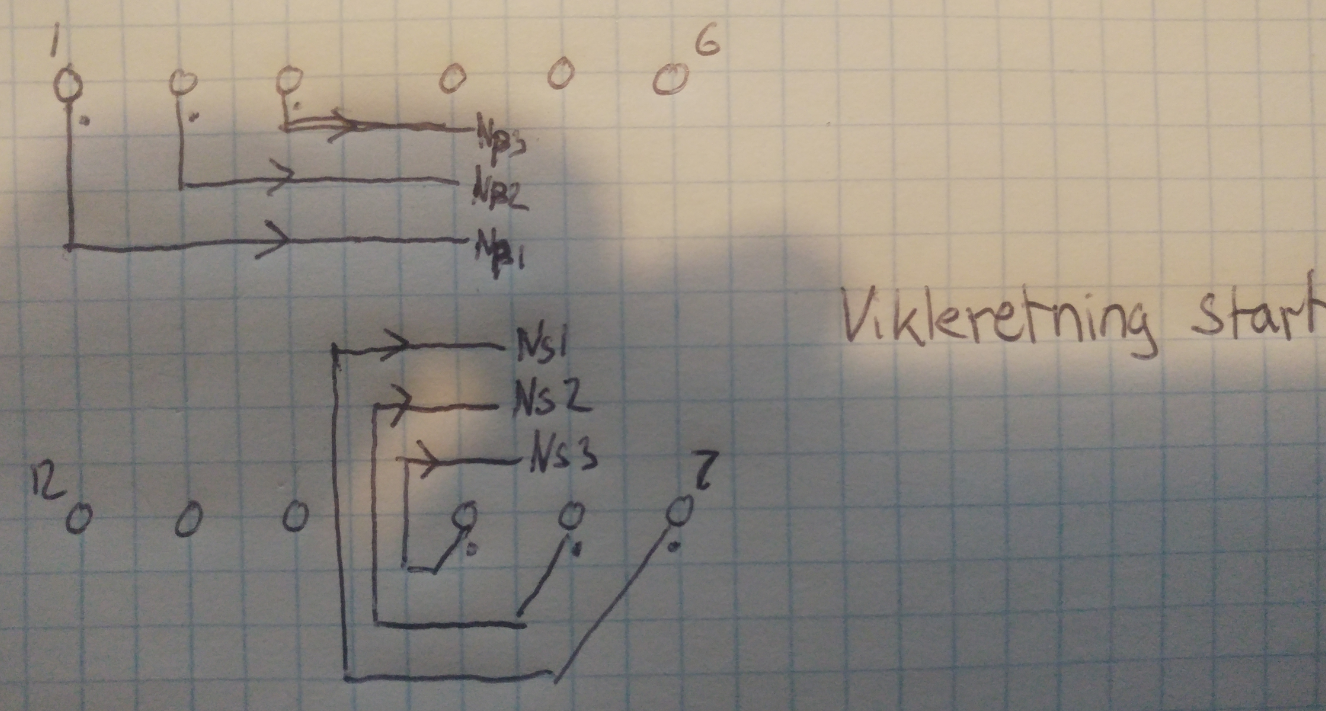
\includegraphics[max width=0.7\linewidth]{/tex/2iteration/billeder/Viklingsretning.png}
	\caption{Begyndelses retning for primær og sekundær}
	\label{fig: viklingsretning}
\end{figure}

\subsection{Realisering}
På figur~\ref{fig: Viklettrans} ses den viklede transformator. Ved viklingen måtte det erkendes, at der ikke kunne realiseres 18 vindinger ind, med en ledningstykkelse på $0.450\milli m$, som ellers i forvejen var mindre end den udregnede tykkelse på $0.478\milli m$. I stedet benyttes en tykkelse på $0.425\milli m$ og der tilføjes en ekstra vikling, så det totale antal vindinger ender på 19 per vikling. 

\begin{figure}[H]
	\center
	\includegraphics[max width=0.5\linewidth]{/tex/2iteration/billeder/Viklet_transformator.PNG}
	\caption{Viklet transformator}
	\label{fig: Viklettrans}
\end{figure}


\subsubsection{Endelig induktans}
Da vindingstallet blev korrigeret til 19, er induktansen lidt højere end beregnet i første omgang. Den endelige induktans i den viklede transformator beregnes til:
\begin{equation} \label{L_2}
L_2 = N^2 \cdot A_L = 57.76\micro H
\end{equation}
Det ændrer igen en smule på ripple- og peak strømmen i transformatoren:
\begin{equation} \label{I_ripple_final}
I_{ripple} = \frac{V_{inmin} \cdot D_{max}}{L_2 \cdot f_s} = 2.01A
\end{equation}
\begin{equation} \label{I_pk_final}
I_{pk} = \frac{V_{out} \cdot I_{out}}{V_{inmin} \cdot D_{maks}} + \frac{I_{ripple}}{2} = 5.53A
\end{equation}

\subsection{Test af transformator}
Transformatoren er testet ved at måle både selvinduktionen i primær- og sekundærviklingerne samt spredningsselvinduktionen. Til dette blev en impedansmåler brugt. 


Til sådan en måling er det vigtigt, at gøre ledningerne så korte som muligt, da der vil skabes yderligere induktans i dem. Derfor ses ved opstillingen på figur~\ref{fig: Transopstilling} de meget korte ledninger samt at der bliver brugt en 4-wire teknik. Det vil sige to ledninger på hver side af det der måles på. Det gør at strømmen kan sendes igennem det ene sæt ledninger, mens der måles med det andet sæt. Da der ikke løber en strøm i måleledningerne, undgås der en fejlmåling, der ellers vil komme fra ledningerne. 

\begin{figure}[H]
	\center
	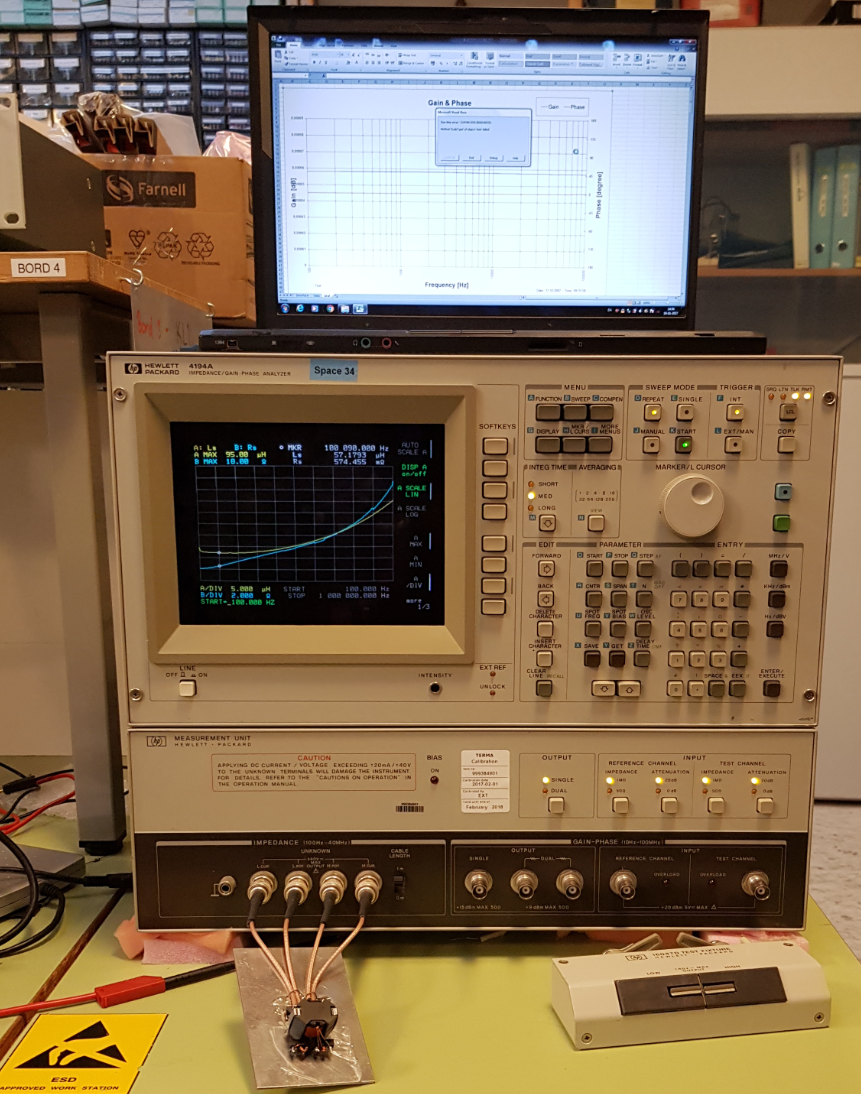
\includegraphics[max width=0.7\linewidth]{/tex/2iteration/billeder/Samlet_transformatortest_opstilling.PNG}
	\caption{Samlet transformatortest opstilling}
	\label{fig: Transopstilling}
\end{figure}

\noindent Måleresultaterne tages med USB ud af impedansmåleren og indsættes i et Excel ark.

\noindent Selve impedansmåleren havde et lille offset på målingerne. Derfor blev der først lavet en kalibreringsmåling, hvor ledningerne alle målte samme sted. Offsettet herfra er i Excel trukket fra de efterfølgende målinger.    

\noindent Herefter måles der på de 2 sider af primærviklingen, mens sekundærsiden holdes åben. På denne måde fås induktansen i den primære vikling. Da transformatoren er 1:1, er det også induktansen i den sekundære vikling. 
\begin{figure}[H]
	\center
	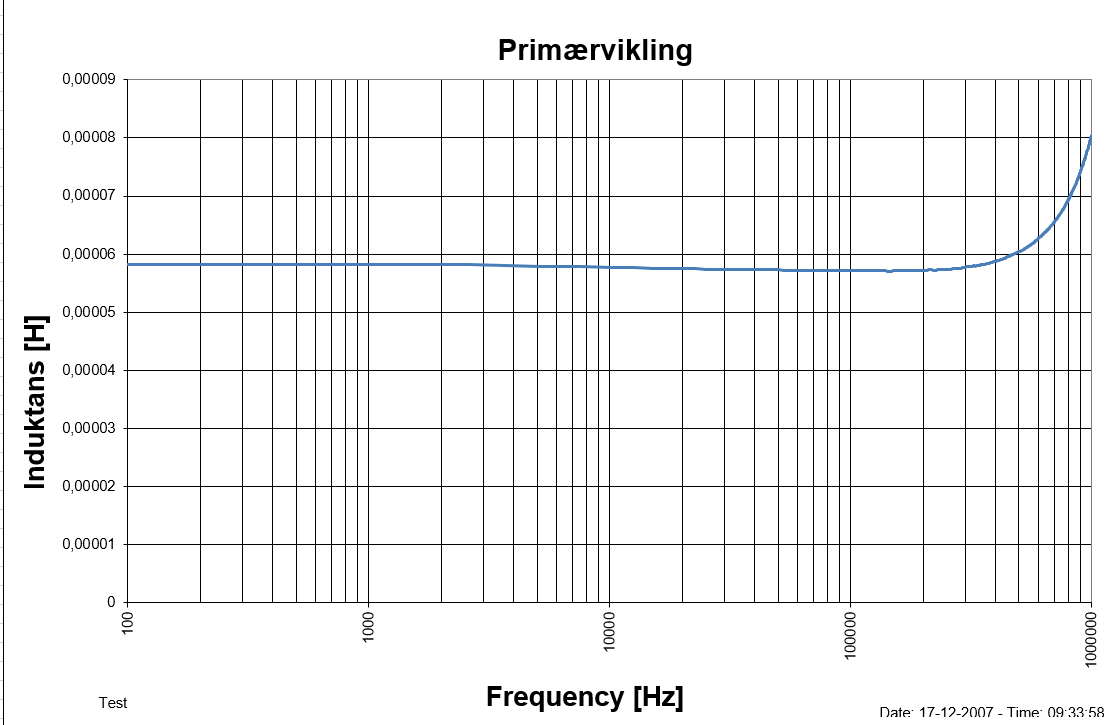
\includegraphics[max width=0.7\linewidth]{/tex/2iteration/billeder/Primarinduktans.png}
	\caption{Målt induktans i primær vikling}
	\label{fig: Primarinduktans}
\end{figure}
\noindent Her er målingen plottet med et frekvenssweep fra $100Hz$ til $1\mega Hz$. Ved de meget høje frekvenser ses det, at kapacitive parasitter tager over. Den skal benyttes ved en switch-frekvens omkring 100kHz og her fås værdien i Excel til $57.7\micro H$, hvilket er præcis den induktans der skulle opnås. Målingerne kan ses i Excel dokumentet ”Inductance primærvikling” i bilagsmappen. 

Spredningsselvinduktionen fås ved, at kortslutte den sekundære vikling, mens der igen måles over den primære vikling. I en ideel transformator bør der her måles 0. Derfor vil induktansen målt her, svare til spredningsselvinduktionen. På samme måde som før er måleresultaterne sendt til Excel hvorudfra en graf kan tegnes. De præcise målinger kan ses i Excel dokumentet ”Spredningsselvinduktion” i bilagsmappen:
\begin{figure}[H]
	\center
	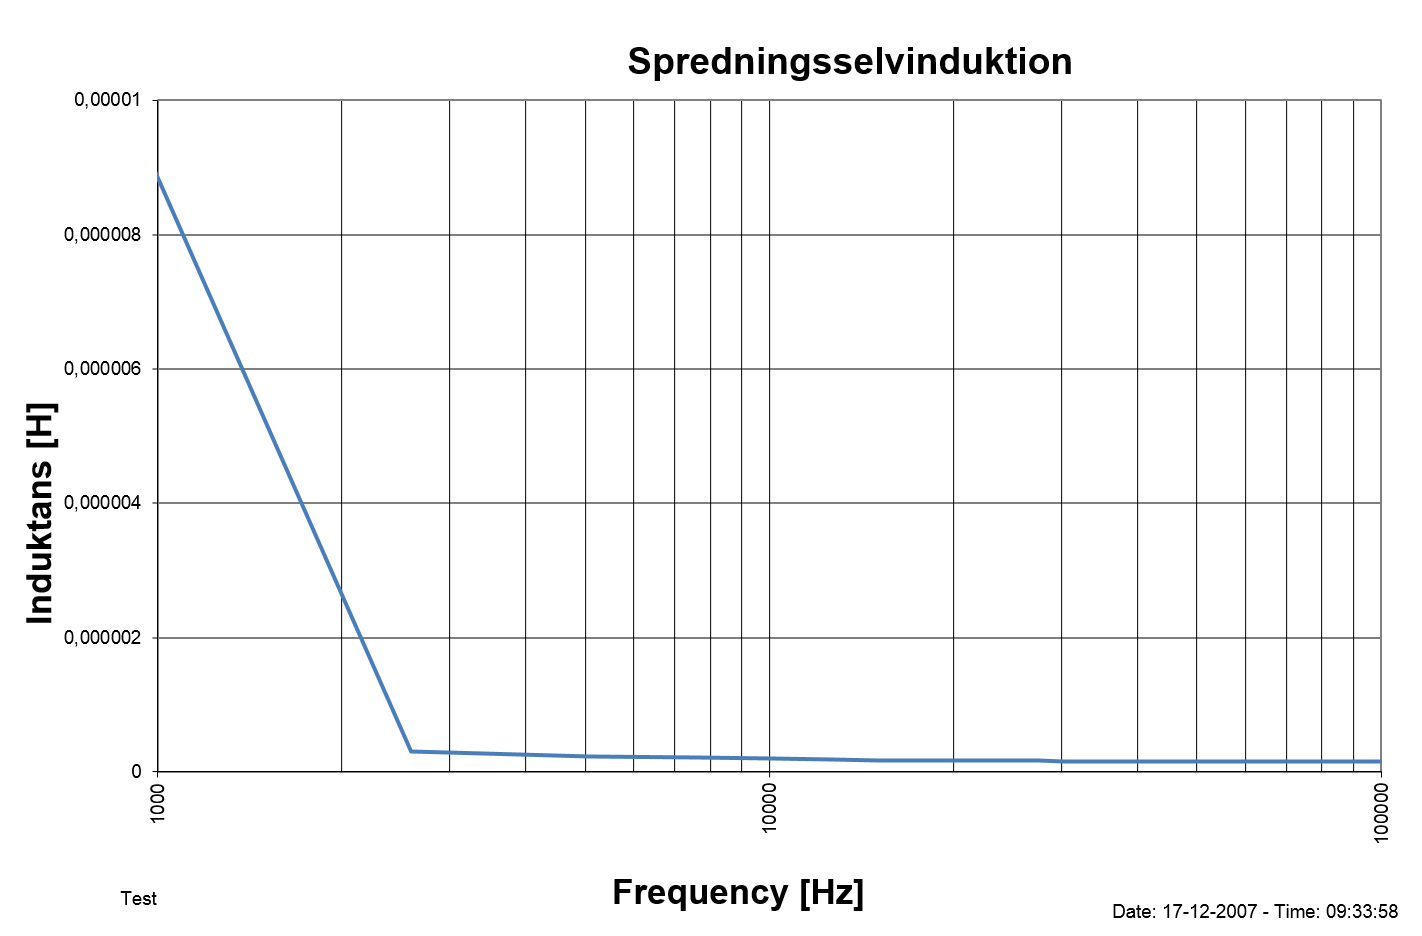
\includegraphics[max width=0.7\linewidth]{/tex/2iteration/billeder/Spredningsselvinduktion.png}
	\caption{Målt spredningsselvinduktion i transformator}
	\label{fig: leakageinductance}
\end{figure}

\noindent Denne graf er fået ud fra et frekvens-sweep fra 1kHz til $100\kilo Hz$. Ved de $100\kilo Hz$ er spredningsselvinduktionen på $152\nano H$, hvilket er den værdi der bruges. 

% Dokumentation af PWM-controller %
% UCC1801 %

\section{PWM-controller} \label{PWM}
PWM-controlleren er en vigtig del af en SMPS. Det er den der står for tilpasningen af switch-signalets duty-cycle, således udgangen holdes stabilt, når inputtet påvirkes eller ændres. Det er vigtigt at vælge PWM-controller ud fra kravene til converteren. PWM-controllere er ofte begrænset til en maksimal duty-cycle på enten $50\percent$ eller $100\percent$. Derudover skal der vælges, hvilken form for regulering af converterens udgangstrin der ønskes, da controlleren skal understøtte dette. 

Ud fra beregningerne af den maksimale duty-cycle i afsnit~\ref{maksimum_duty_cycle}, vælges det at PWM-controlleren maksimalt skal have en duty-cycle på $50\percent$. For at kunne opnå en mere præcis regulering, vælges det at bruge peak-current regulering. Denne form for regulering, regulerer efter peak-strømmen i transformatorens primærvikling. Da den regulere efter dette, opnås der også en strømbegrænser i regulerings-loopet. Ud fra disse krav vælges en PWM-controller af typen UCC1801\cite{UCC1801}. Det er en controller Terma har erfaring med, og derfor også nemt kan udskiftes med en space-godkendt controller.

\subsection{Funktionalitet}
På figur~\ref{fig:PWM_block_diagram} ses et funktionelt block diagram over UCC1801. Det indeholder controllerens overordnede komponenter, og giver et overblik over dens funktionalitet. 

\begin{figure}[H]
	\center
	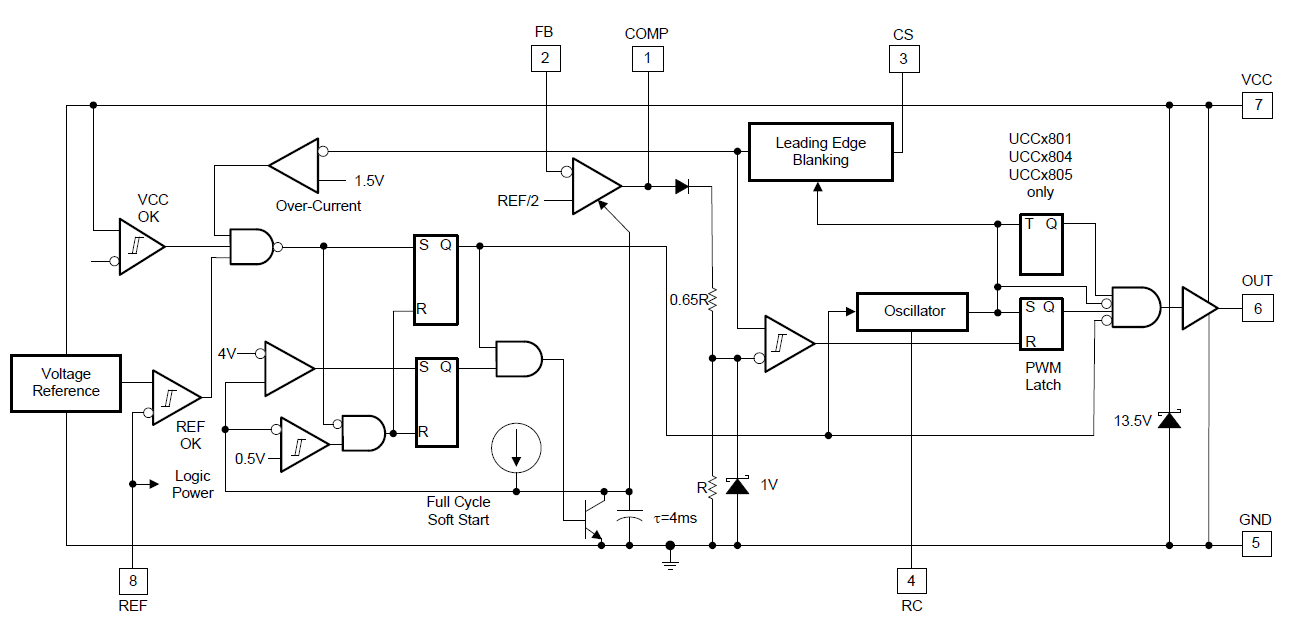
\includegraphics[max width=0.9\linewidth]{/tex/2iteration/billeder/PWM_block_diagram.PNG}
	\caption{UCC1801 - Funktionelt Block Diagram}
	\label{fig:PWM_block_diagram}
\end{figure}

Tabel~\ref{tab:ucc1801_specs} viser de mest essentielle specifikationer for UCC1801, i forhold til en flyback converter. Disse er udvalgte specifikationer fra databladet.

\begin{table}[H] 			
	\centering
	\begin{tabularx}{\textwidth}{|X|c|c|c|} 
		\hline
		\textbf{Specifikation} & \textbf{Min} & \textbf{Typ} & \textbf{Max} \\ \hline
		$V_{CC}$ &  &  & $12V$ \\ \hline
		$I_{out}$ &  &  & $1A$ \\ \hline
		$V_{Reference}$ & $4.925V$ & $5V$ & $5.075V$ \\ \hline
		$D_{max}$ & $48\percent$ & $49\percent$ & $50\percent$ \\ \hline
		$V_{on,th}$ & $8.6V$ & $9.4V$ & $10.2V$ \\ \hline
		$V_{off,th}$ & $6.8V$ & $7.4V$ & $8V$ \\ \hline
		Temperature Range & $-55\degreeCelsius$ &  & $125\degreeCelsius$ \\ \hline
		$f_{osc}$ & & & $1M\hertz$ \\ \hline
	\end{tabularx}

	\caption{Relevante specifikationer for UCC1801}
	\label{tab:ucc1801_specs}
\end{table}


\subsubsection{Ben konfiguration}
Der tages udgangspunkt i en UCC1801, med en PDIP pakke type. Figur~\ref{fig:ucc1801_pin_overview} viser en oversigt over ben konfigurationen for en sådan pakke. Det er en 8-bens IC, hvor samtlige ben bliver brugt. Benenes funktionalitet er overordnet beskrevet i tabel~\ref{tab:ucc1801_pin_functionality}, og vil blive uddybet i de følgende afsnit.

\begin{figure}[H]
	\center
	\includegraphics[max width=0.7\linewidth]{/tex/2iteration/billeder/ucc1801_pin_overview.PNG}
	\caption{Ben konfiguration for UCC1801}
	\label{fig:ucc1801_pin_overview}
\end{figure}

\begin{table}[H] 			
	\centering
	\begin{tabularx}{\textwidth}{|c|c|c|X|} 
		\hline
		\textbf{Navn} & \textbf{Ben} & \textbf{I/O} & \textbf{Beskrivelse} \\ \hline
		COMP & 1 & O & COMP er outputtet fra den indbyggede fejlforstærker. Dette ben bruges til at lave et feedback til FB benet i reguleringssløjfen. 	\\ \hline
		FB 	 & 2 & I & FB er inputtet til den indbyggede fejlforstærker. Den er forbundet til den inverterende indgang af forstærkeren. Den bruges sammen med COMP, som en del af reguleringssløjfen.\\ \hline
		CS   & 3 & I & CS er inputtet til current sense komparatorne. UCC1801 har to komparatorere til current sense: PWM komparatoren og overstrøms komparatoren. PWM-komparatoren bruges til, at trække udgangssignalet lavt, når CS-signalet overstiger $1V$. Overstrøms komparatoren er en indbygget overstrømsbeskyttelse. Den tvinger udgangen lav, så længe CS-signalet er over $1.5V$ \\ \hline
		RC 	 & 4 & I & RC er inputtet til oscillatoren. Oscillator frekvensen, og dermed også switch-frekvensen, sættes ud fra tidskonstanten mellem en modstand og en kondensator.  \\ \hline
		GND  & 5 & - & GND er ground for IC'ens komponenter.  \\ \hline
		OUT  & 6 & O & OUT er IC'ens output. Det er et PWM-signal, hvis duty-cycle afhænger af PWM-komparatoren. Outputtet skiftes mellem GND og VCC, hvilket betyder at VCC skal være høj nok, til at drive MOSFET'en.  \\ \hline
		VCC  & 7 & I & VCC er forsyning til IC'ens komponenter. Det foreslås at vælge en høj VCC, for at mindske støjpåvirkninger. For at mindske støj på forsyningen anbefales det, at bypasse VCC med en kondensator på minimum $1\micro \farad$, tæt på IC'en. \\ \hline
		REF  & 8 & O & REF er outputtet for IC'ens interne spændingsreference. Den bruges bl.a. som reference til fejlforstærkeren. Derudover forsyner den IC'ens logiske komponenter. For at mindske støj på referencen, anbefales det at bypasse REF med en kondensator på minimum $1\micro \farad$, tæt på IC'en. \\ \hline
	\end{tabularx}
	
	\caption{Ben funktionalitet for UCC1801}
	\label{tab:ucc1801_pin_functionality}
\end{table}

\subsection{Under Voltage LockOut}
UCC1801 indeholder en Under Voltage LockOut (UVLO) beskyttelse. Dette betyder at forsyningsspændingen skal være et bestemt niveau, før controlleren starter. Som en konsekvens af dette vil både outputtet og referencespændingen holdes lav, indtil grænseværdien er nået. For at have en hysteresemargin, har den både et turn ON og et turn OFF niveau. Ved UCC1801 er disse niveauer $V_{on,th}=9.4V$ og $V_{off,th}=7.4V$. Da amplituden af output-signalet er lig VCC, vil controlleren ikke prøve at drive MOSFET'en før $V_{CC}=9.4V$. Da en MOSFET typisk har en $V_{gs,th}$ mellem $4$ og $5V$, vil der ikke opnås et stadie hvor MOSFET'en kun er delvist ON. Dette ses også på referencespændingen, da den først bliver $5V$ når $V_{CC}\geqslant 9.4V$. Referencen kan derfor også bruges, som en ON/OFF indikator. 

\subsection{Switch-frekvens}
Controllerens switch-frekvens sættes af oscillator blokken i block diagrammet. Den genererer en savtand-spænding, som trigger den efterfølgende latch. Dette giver et PWM-signal, da det skifter mellem VCC og GND.
Stigetiden for savtand spændingen bliver bestemt af tidskonstanten for et eksternt RC-kredsløb. Faldetiden for signalet bliver bestemt af den eksterne kondensator, samt ON-modstanden i en intern transistor. Den on-modstand er opgivet til ca. $130\ohm$. Denne faldetid vil begrænse den maksimale duty-cycle, da outputtet vil være lavt i løbet af faldetiden. 

\begin{figure}[H]
	\center
	\includegraphics[max width=0.7\linewidth]{/tex/2iteration/billeder/PWM_oscillator_diagram.PNG}
	\caption{Oscillator diagram}
	\label{fig:PWM_oscillator_diagram}
\end{figure}

Figur~\ref{fig:PWM_oscillator_diagram} viser et ækvivalent diagram for oscillator blokken. Komponenterne $R_T$ og $C_T$ er det eksterne RC kredsløb, mens resten er interne komponenter. På diagrammet ses det at operationsforstærkerne er koblet til henholdsvis $0.2V$ og $2.65V$. Dette sætter maksimum og minimum for savtand spændingen. 

Da der skal komme en flanke på output-signalet hver gang savtand spændingen rammer maksimum, skal frekvensen af savtand spændingen være den dobbelte af den ønskede switch-frekvens. Der ønskes en switch-frekvens på $100k\hertz$, derfor sættes oscillator frekvensen til $f_{osc}=200k\hertz$. I databladet er det anbefalet at $R_T$ vælges mellem $10k\ohm$ og $200k\ohm$, mens det anbefales at $C_T$ vælges mellem $100p\farad$ og $1000p\farad$. Formel~\ref{f_osc} er opgivet i databladet og bruges til at estimere RC komponenterne. $C_T$ sættes til $200p\farad$, og $R_T$ beregnes:
\begin{equation} \label{f_osc}
R_{T} = \frac{1.5}{f_{osc} \cdot C_T} = \frac{1.5}{f_{osc} \cdot C_T} = 37.5k\ohm
\end{equation}
Ved et opslag i databladet ses det, at med en $C_T=200p\farad$ kan der maksimalt opnås en duty-cycle på ca. $48.9\percent$. Da converteren maksimalt skal opererer med en duty-cycle på $44.7\percent$, godtages dette.

\subsection{Current sense kredsløb} \label{CS_loop}
Som nævnt i afsnit~\ref{PWM} er der valgt at bruge peak-current regulering. Denne form for regulering består af to reguleringssløjfer - en spændings- og en strømsløjfe. I dette afsnit beskrives dimensioneringen af strøm sløjfen, mens spændingssløjfen beskrives i afsnit~\ref{V_loop}.

Current sense kredsløbet består, som minimum, af en current sense modstand. Denne modstand bruge til at konvertere strømmen i transformatorens primærvikling om til en spænding. Denne konvertering vil gøre, at kurveformen for strømmen og spændingen er ens, dog med en faktor til forskel. PWM-komparatoren i controlleren trigger udgangen, når current sense spændingen er rampet op til $1V$. Derfor skal modstanden dimensioneres således, spændingen over den er lig $1V$ når peak-strømmen i transformatoren er lig $5.53A$. Dette regnes ud fra Ohm's lov:
\begin{equation} \label{R_cs}
R_{cs} = \frac{1V}{5.53A} = 0.181\ohm
\end{equation}

Da den mindste modstandsværdi der er til rådighed er på $1\ohm$, vil der blive brugt $6\cdot 1\ohm$ i parallel. Dette vli give en modstandsværdi på $0.167\ohm$. 



\subsubsection{Filtrering}
På grund af switching-spikes i MOSFET'en, når den går ON, vil der også komme spikes på current sense signalet. Hvis disse spikes når et niveau der er højere end $1V$, vil det trigger komparatoren. Dette vil få controlleren til at generer et PWM-signal, der er meget lavere end det ønskede. Derfor implementeres der et filter, for at filtrere disse spikes væk.

UCC1801 har et indbygget digitalt filter, kaldet Leading Edge Blanking. Dette filter er designet til at filtrere de første $100ns$ af signalet væk, og dermed fjerne spiken. Ideelt set vil dette give et signal, som ses på figur~\ref{fig:ucc1801_leading_edge}.

\begin{figure}[H]
	\center
	\includegraphics[max width=0.7\linewidth]{/tex/2iteration/billeder/ucc1801_leading_edge.PNG}
	\caption{Current sense signal før og efter Leading Edge Blanking}
	\label{fig:ucc1801_leading_edge}
\end{figure}

Det digitale filter er ikke altid tilstrækkeligt, og derfor designes et eksternt analogt RC-filter, for yderligere filtrering. Det designes til at have en stige tid på $300ns$, for at tilføje en yderligere filtrering på ca. $200ns$. 

\noindent Med en stige tid på $300ns$, kan båndbredden af filteret estimeres:
\begin{equation} \label{filter_BW}
BW \approx \frac{0.34}{t_r} \approx 1.133M\hertz
\end{equation}

\noindent Der vælges en kondensator på $C_f=100pF$. Ud fra kondensatoren og den ønskede båndbredde i filteret, regnes modstanden.
\begin{equation} \label{filter_R}
R_f = \frac{1}{2 \cdot \pi \cdot BW \cdot C_f} = 1.4k\ohm
\end{equation}

Med det designede filter vil stige tiden af current sense signalet, nu blive begrænset af filteret. Derfor vil den første de af signalet nu ligne et første ordens system, der stiger indtil spændingen når det niveau der svarer til strømmen i primærviklingen. Derefter vil signalet stige som en ret linje, ligesom strømmen. Dette ses på figur~\ref{fig:ucc1801_CS_filter}, hvor det øverste signal er før filteret, og det nederste er efter.

\begin{figure}[H]
	\center
	\includegraphics[max width=0.7\linewidth]{/tex/2iteration/billeder/ucc1801_CS_filter.PNG}
	\caption{Current sense signal før og efter eksternt RC-filter}
	\label{fig:ucc1801_CS_filter}
\end{figure}

\subsubsection{Overstrømsbeskyttelse} \label{CS_protection}
En fordel ved, at regulere efter strømmen i transformatoren er, at der opnås en overstrømsbeskyttelse. Når strømmen stiger, vil PWM-controlleren sænke duty-cyclen, og derved også sænke udgangsspændingen. Dette giver en I/V karakteristik der, ideelt set, er næsten firkantet. Dette er skitseret på figur~\ref{fig:I-V_karateristik}. 

\begin{figure}[H]
	\center
	\includegraphics[max width=0.7\linewidth]{/tex/2iteration/billeder/I-V_karakteristik.PNG}
	\caption{I/V karakteristik for converteren}
	\label{fig:I-V_karateristik}
\end{figure}

Denne karakteristik kan dog ikke opnås i realiteten. Filteret der er indsat for at filtrere current sense signalet, vil lave en hale på karakteristikken. Det sker fordi controlleren ikke ser den faktiske strøm, men den filtrerede, når duty-cyclen er lav. 

Da det er nødvendigt at filtrere current sense signalet, men samtidig påvirker converterens I/V karakteristik, optimeres filteret ofte således, det kun akkurat filtrer nok. Denne optimering vil ske i 3. iteration. 

\subsection{Spændingsregulering} \label{V_loop}
I dette afsnit beskrives spændingssløjfen. Den består hovedsageligt af to dele: en spændingsdeler og en fejlforstærker. Spændingsdeleren deler udgangsspændingen ned, så den ønskede udgangsspænding er lig en intern reference i IC'en. Fejlforstærkeren står for selve reguleringen. Den inverterende indgang og udgangen på fejlforstærkeren er ført ud, således det er muligt at indsætte et kompenseringsnetværk.

\subsubsection{Spændingsdeler}
Den ikke inverterende indgang på den indbyggede fejlforstærker i UCC1801, er forbundet til den halve reference spænding, dvs. $2.5V$. Derfor skal der designes en spændingsdeler, der deler den ønskede udgangsspænding på $21V$ ned til $2.5V$. Figur~\ref{fig:Voltagedivider_ideal} viser kredsløbet for spændingsdeleren. 

\begin{figure}[H]
	\center
	\includegraphics[max width=0.7\linewidth]{/tex/2iteration/billeder/Voltagedivider_ideal.PNG}
	\caption{Spændingsdeler diagram}
	\label{fig:Voltagedivider_ideal}
\end{figure}

Spændingsdeleren designes således der løber en strøm på $1mA$ i den. Derved påvirker den ikke udgangsstrømmen. Derudover dimensioneres de to modstande, således der er et spændingsfald på $2.5V$ over $R_{FB2}$, og $21V-2.5V$ over $R_{FB1}$. $R_{FB1}$ er beregnet med ligning~\ref{RFB1}.

\begin{equation} \label{RFB1}
R_{FB1} = \frac{V_{out}-V_{FB}}{I_{FB1}} = \frac{21V-2.5V}{1mA} = 18.5k\ohm
\end{equation}

\noindent $R_{FB2}$ er beregnet ud fra spændingsdeler formlen, ligning~\ref{RFB2}. Her løses $R_{FB2}$, og fås til $R_{FB2}=2.527k \ohm$.  
\begin{equation} \label{RFB2}
V_{FB} = \frac{R_{FB2}}{R_{FB1} + R_{RB2}} \cdot V_{out}
\end{equation}

For at opnå en præcis spændingsdeler vælges der at bruge to modstande i parallel. Den ene modstand vælges til $R_{FB21}=2.55k\ohm$. Mens den anden regnes ud fra den ønskede samlede modstandsværdi. Dette gøres ved ligning~\ref{RFB22}, som løses med hensyn til $R_{FB22}$. Dette giver $R_{FB22}=280.5k\ohm$, som afrundes til $280k\ohm$.
\begin{equation} \label{RFB22}
R_{FB2} = ((R_{FB21})^{-1} + (R_{FB22})^{-1})^{-1}
\end{equation}

\subsubsection{Fejlforstærker}
Som en del af reguleringen opstilles der først en overføringsfunktion for power-modulet. Denne overføringsfunktion er opgivet i databladet for UCC1801, og er skrevet ved ligning~\ref{H_Power}.
\begin{equation} \label{H_Power}
G_{pwr}(s) = G_0 \cdot \frac{(1+\frac{s}{2\pi \cdot f_{ESRz}}) \cdot (1-\frac{s}{2\pi \cdot f_{RHPz}})}{1+\frac{s}{2\pi \cdot f_{p1}}} \cdot \frac{1}{1 + \frac{s}{2\pi \cdot f_{p2}} + \frac{s^2}{(2\pi \cdot f_{p2})^2}}
\end{equation}

Overføringsfunktionen består af flere dele: en DC-forstærkning, to poler og to nulpunkter. DC-forstærkningen, $G_0$, er skrevet ved ligning~\ref{DC_gain}. Den er især bestemt af belastningen, current sense kredsløbet, transformatoren og switch-frekvensen. Den regnes til en forstærkning på $10.74$ gange, eller $20.6\decibel$.
\begin{equation} \label{DC_gain}
G_0 = \frac{R_{out} \cdot N}{R_{CS} \cdot A_{CS}} \cdot \frac{1}{\frac{(1-D)^2}{\tau_L} + (2 \cdot M) + 1} = 10.7GG \Rightarrow 20.6\decibel
\end{equation}
\noindent Hvor:
\newline \noindent $N$ er omsætningsforholdet i transformatoren.
\newline \noindent $A_{CS}$ er den interne forstærkning i current sense kredsløbet, og aflæses i databladet til $1.65$.
\newline \noindent $D$ er den maksimale duty-cycle, som er $0.447$.
\newline \noindent $\tau_L$ er converterens tidskonstant. Den regnes ud fra ligning~\ref{tau_L}.
\begin{equation} \label{tau_L}
\tau_L = \frac{2 \cdot L_P \cdot f_s}{R_{out} \cdot N^2}
\end{equation}
\newline \noindent $M$ er spændingsomsætningen fra indgang til udgang. Den regnes ud fra ligning~\ref{M}.
\begin{equation} \label{M}
M = \frac{V_{out} \cdot N}{V_{in}}
\end{equation}

En flyback converter, som opererer i CCM, har to primære nulpunkter der kan påvirke stabiliteten i systemet. Det er også de to nulpunkter der er inkluderet i overføringsfunktionen. Den ene, $f_{ESRz}$, er bestemt af produktet mellem udgangskapaciteten og den indre seriemodstand i udgangskondensatoren. Placeringen af denne er regnet ved ligning~\ref{ESR_zero}.
\begin{equation} \label{ESR_zero}
f_{ESRz} = \frac{1}{2 \cdot \pi \cdot R_{ESR} \cdot C_{out}} = 189.5k\hertz
\end{equation}

Det andet nulpunkt er højre-halvplans-nulpunktet. Det er ofte dette nulpunkt der er det dominerende af de to, og derfor den der skal tages højde for i reguleringen. Placeringen af dette er regnet ved ligning~\ref{RHP_zero}. Placeringen af dette nulpunkt, er afhængigt af størrelsen på belastningen, samt inputspændingen. Placeringen stiger ved højere inputspændinger, og mindre belastninger. 
\begin{equation} \label{RHP_zero}
f_{RHPz} = \frac{R_{out} \cdot (1-D)^2 \cdot N^2}{2 \cdot \pi \cdot L_P \cdot D} = 15.8k\hertz
\end{equation}

\noindent Ud fra ligning~\ref{ESR_zero} og \ref{RHP_zero}, ses det, at det er højre-halvplans nulpunktet der er det dominerende nulpunkt i converteren. Når båndbredden skal vælges, er det derfor vigtigt, at den ligger tilpas meget lavere end det dominerende nulpunkt.

Converteren har også to relevante poler. Den dominerende pol bestemmes af load'en og udgangskondensatoren. Den anden pol er placeret ved den halve switching-frekvens. De to poler er beregnet ved ligning~\ref{pol1} og \ref{pol2}.
\begin{equation} \label{pol1}
f_{p1} = \frac{\frac{(1-D)^3}{\tau_L} + 1 + D}{2\cdot \pi \cdot R_{out} \cdot C_{out}} = 132.8\hertz
\end{equation}

\begin{equation} \label{pol2}
f_{p2} = \frac{f_s}{2} = 50k\hertz
\end{equation}

\noindent Bode plottet for power-modulet plottes i MATLAB på figur~\ref{fig:MATLAB_power_module}. Her aflæses DC-forstærkningen til $20.6\decibel$. Derudover aflæses der en pol ved ca. $130\hertz$ og ved ca. $50k\hertz$. Dette stemmer overens med de beregnede værdier.

Konsekvensen af højre-halvplans nulpunktet ses også tydeligt på figur~\ref{fig:MATLAB_power_module}. Når frekvensen nærmer sig nulpunktet bliver forstærkningen øget med $20 \decibel$/decade, som ved et venstre-halvplans nulpunkt. Tilgengæld vil fasen blive trukket ned med $90^\circ$, i stedet for op. Da polen fra switch-frekvensen ligger ca. samme sted, og også trækker fasen ned med $90^\circ$, kommer der et stort fasedrej i dette frekvensområde. Det kan gøre systemet ustabilt hvis gain-marginen ikke er tilstrækkelig stor. 

\begin{figure}[H]
	\center
	\includegraphics[max width=0.7\linewidth]{/tex/2iteration/billeder/MATLAB_power_module.PNG}
	\caption{Bode plot for power-modulet}
	\label{fig:MATLAB_power_module}
\end{figure}

I denne iteration designes der et kompensationsnetværk der vil sikre et stabilt system, med en lav båndbredde. Dette vil blive optimeret i en senere iteration. 
Da der ønskes en lavere båndbredde, end det converteren har i forvejen, indsættes et RC-led i serie som kompensationsnetværk. Ved at bruge et RC-led, vil kondensatoren bestemme forstærkningen ved lave frekvenser, fordi impedansen her er stor. Mens modstanden vil bestemme forstærkningen ved høje frekvenser, fordi kondensatoren vil blive set som en kortslutning. 

Den endelige båndbredde af systemet ønskes på ca. $800\hertz$. Det vil sikre, at systemet ikke bliver ustabilt. For at opnå den ønskede båndbredde aflæses det ud fra bode plottet på figur~\ref{fig:MATLAB_power_module}, at forstærkningen skal mindskes med ca. $5.4\decibel$, eller ca. $0.535GG$, ved frekvenser over $800\hertz$. Den samlede forstærkning af reguleringssløjfen, bestemmes af produktet mellem forstærkningen i spændingsdeleren og forstærkningen i fejlforstærkeren. Forstærkningen i spændingsdeleren regnes ved ligning~\ref{voltagedivider_gain}.
\begin{equation} \label{voltagedivider_gain}
g_{FB} = \frac{R_{FB2}}{R_{FB1}+R_{FB2}} = 0.12
\end{equation}

\noindent Nu kan feedback modstanden i fejlforstærkeren regnes ved ligning~\ref{error_opamp_gain}. 
\begin{equation} \label{error_opamp_gain}
g_{tot} = \frac{R_{comp}}{R_{par}} \cdot g_{FB}
\end{equation}

\noindent Hvor:
\newline \noindent $g_{tot}$ er det ønskede gain i fejlforstærkeren, som er $g_{tot}=0.535GG$.
\newline \noindent $R_{comp}$ er feedback modstanden i fejlforstærkeren, som ønskes dimensioneret.
\newline \noindent $R_{par}$ er parallelmodstanden mellem $R_{FB1}$ og $R_{FB2}$. Den regnes til $R_{par}=2.244k\ohm$.

\noindent De kendte værdier indsættes og ligningen løses for $R_{comp}$. Den fås til $R_{comp}\approx 10k\ohm$.


\noindent For at sikre en den lave båndbredde, sættes knækfrekvensen på integratoren til $f_0=300\hertz$. Dermed sikres det, at fejlforstærkeren dæmper signalet ved den ønskede båndbredde på $800\hertz$. Nu den tilhørende kapacitet regnes, ud fra $R_{comp}$ og $f_0$.
\begin{equation} \label{c_comp}
c_{comp} = \frac{1}{2\cdot \pi \cdot R_{comp} \cdot f_0} \approx 50nF
\end{equation}

\noindent Med afrundede komponentværdier, regnes den nye knækfrekvens for fejlforstærkeren.
\begin{equation} \label{f_0}
f_0 = \frac{1}{2\cdot \pi \cdot R_{comp}} \cdot c_{comp} = 318.3\hertz
\end{equation}

\noindent Overføringsfunktionen for fejlforstærkeren kan nu opskrives ved ligning~\ref{H_err}.
\begin{equation} \label{H_err}
G_{err}(s) = (\frac{318.3\hertz \cdot 2\cdot\pi}{s} + 1) \cdot 0.535
\end{equation}

\noindent Den plottes i MATLAB, som et bode plot på figur~\ref{fig:MATLAB_error_op_amp_2}. Her ses det, at den ønskede funktion af integratoren er opnået. På grund af kondensatoren, har den et stort gain ved lave frekvenser. Mens forstærkningen ligger konstant ved ca. $-5.4\decibel$, efter den ønskede knækfrekvens på ca. $318\hertz$.

\begin{figure}[H]
	\center
	\includegraphics[max width=0.7\linewidth]{/tex/2iteration/billeder/MATLAB_error_op_amp.PNG}
	\caption{Bode plot for fejlforstærker}
	\label{fig:MATLAB_error_op_amp_2}
\end{figure}

De to overføringsfunktioner ganges sammen for, at bestemme den samlede overføringsfunktion for converteren. Figur~\ref{fig:MATLAB_total_2} viser et åben sløjfe bode plot af det. Det aflæses at converteren vil have en båndbredde på $810\hertz$. Derudover aflæses fase-margin til $74.3^\circ$, og gain-margin til $24\decibel$.

\begin{figure}[H]
	\center
	\includegraphics[max width=0.7\linewidth]{/tex/2iteration/billeder/MATLAB_total.PNG}
	\caption{Bode plot for converteren}
	\label{fig:MATLAB_total_2}
\end{figure} 






\section{MOSFET} \label{MOSFET}
MOSFET'en skal først og fremmest kunne holde til den spænding, der vil ligge over drain-source, når den er OFF. Ved en flyback er det den maksimale indgangsspænding plus den spænding der bliver reflekteret tilbage til primærviklingen fra sekundærviklingen. Det vil sige udgangsspændingen samt diodens spændingsfald. Den reflekterede spænding skal ganges med omsætningsforholdet i transformatoren, som i dette tilfælde er 1. Det vil ideelt set betyde, at MOSFET'en skal kunne holde til:
\begin{equation} \label{Vds_breakideel}
Vds_{breakideel} = (V_{inmax}+(V_{out}+V_D))= 71.5V
\end{equation}
Der bør medtages en sikkerhedsmargin på $30\percent$, for at tage højde for de peakspændinger, der vil komme når der switches. De skyldes kombinationen af spredningsselvinduktionen og kapaciteterne fra MOSFET og diode. Derudover vil der også være kapacitet grundet transformatorens kobling. Typisk vil MOSFET og diodens kapaciteter være større og dermed dominerende. Tages der højde for disse spændingstransienter skal MOSFET'en minimum kunne holde til en spænding på: 
\begin{equation} \label{Vds_break}
Vds_{break} = (V_{inmax}+(V_{out}+V_D)) \cdot 1.3 = 92.95V
\end{equation}

Yderligere skal den valgte MOSFET kunne holde til RMS strømmen i primærviklingen på $3.02A$ samt peakstrømmen på $5.64A$.
Til 2. iteration er IRFB23N15 valgt\cite{IRFB23N15}. Den kan holde til $V_{ds}$ på $150V$ og en continous drain strøm på $17A$ samt en peak på $92A$, hvilket er rigeligt. Derudover en $R_{ds(on)}$ modstand på ca. $113\milli \ohm$ ved $50\degreeCelsius$. 

\subsection{Switch-tid}
MOSFET'ens switch-tid bestemmes af den strøm der løber i gaten. MOSFET'en indeholder flere parasitiske kapaciteter, mellem gate-drain og gate-source. Hvor opladningen af gate-drain, også kaldet \textit{Miller} kapaciteten, bestemmer hvor hurtigt MOSFET'en kan skifte tilstand fra OFF til ON. I switch-tiden vil der både løbe en strøm i MOSFET'en og ligge en spænding over den. Dette vil give anledning til et tab kaldet switch-tab. Princippet i tabet er skitseret på figur~\ref{fig:MOSFET_switch_tid}. Her ses det, at når gate spændingen går høj, skifter MOSFET'en ikke momentant. Det er først når strømmen er rampet op, spændingen begynder at falde. Da effekten er produktet mellem strøm og spænding, vil dette skabe energitrekanter, hvor længden af dem er lig switch-tiden. Den tid ønskes derfor kort, for at mindske switch-tabet. 


\begin{figure}[H]
	\center
	\includegraphics[max width=0.7\linewidth]{/tex/2iteration/billeder/MOSFET_switch_tid.png}
	\caption{Effekttrekanter for MOSFET}
	\label{fig:MOSFET_switch_tid}
\end{figure}

Gate modstanden regnes ved at løse ligning~\ref{R_g_2}\cite{gate_res}. Her er $T_{ch}$ den ønskede switch-tid, som sættes til ca. $150ns$. $Q_{gd}$ er gate-drain ladningen, som afhænger af Miller kapaciteten, den aflæses i databladet til typisk $19nC$. $V_{DD}$ er forsyningsspændingen til PWM-controlleren på $12V$, og dermed også den maksimale spænding af udgangssignalet. $V_{gs}$ er spændingsfaldet fra gate til source for MOSFET'en. Med en drain strøm på $3A$ bliver $V_{gs}\approx 5V$. Dette indsættes og ligningen løses med hensyn til $R_{g}$, som fås til $R_{g}=55.3\ohm$. Der vælges en modstand på $51.1\ohm$. Med den valgte modstand korrigeres switch-tiden til $138.7ns$.

\begin{equation} \label{R_g_2}
T_{ch} = \frac{Q_{gd} \cdot R_{g}}{V_{DD}-V_{gs}}
\end{equation}

\section{Diode}
For at mindske tabet i konverteren skal spændingsfaldet over dioden helst være så lille som muligt. Der skal dog sørges for, at dioden kan holde til den spænding, der ligger over den, når transistoren er ON. Denne breakdown voltage er ideelt se den maksimale indgangsspændingen plus udgangsspændingen.
\begin{equation} \label{Vd_breakideel}
Vd_{breakideel} = (V_{out}+V_{inmax}) = 71V
\end{equation}
Igen skal der i realiteten tages højde for peakspændinger ligesom ved MOSFET'en. Der ganges derfor igen en faktor 1.3 på, og dioden skal dermed kunne holde til spændingen:
\begin{equation} \label{Vd_break}
Vd_{break} = (V_{out}+V_{inmax}) \cdot 1.3 = 92.3V
\end{equation}
Yderligere skal dioden kunne holde til RMS strømmen på udgangen på de $3.36A$ og en peakstrøm på $5.53A$.

Schottky dioden NTSV30120CT\cite{NTSV30120} er valgt til 2. iteration med en breakdown voltage på $120V$. Dioden kan klare en continuos strøm på $5A$ og en peakstrøm på $30A$ per device. Hele pakken er med 2 dioder, og da der her kun benyttes én af dem, er det i stedet en peakstrøm på $15A$, der er maksimum. Derudover kan dens spændingsfald aflæses i databladet til ca. $0.45V$ ved $125\degreeCelsius$ og $2.5A$. 


\section{Udgangskondensator} \label{output_cap}
Som udgangskondensator er valget faldet på 4 parallelle kondensatorer på $56\micro F$ af typen . Dette var den film kondensator med højest kapacitet Terma havde til rådighed. Det vigtige her, er at det er en film kondensator, da de typisk har ret præcise kapaciteter samt en lav ESR modstand. Når kondensatorer ikke længere anses som ideele, vil der i virkeligheden både være en ESL induktans og en ESR modstand. Ækvivalentdiagrammet for en kondensator vil derfor se ud som på figur~\ref{fig: con_equi} 
%TODO: Indsæt kondensator type, og reference til datablad
\begin{figure}[H]
	\center
	\includegraphics[max width=0.7\linewidth]{/tex/2iteration/billeder/Kondensator_equivalent.png}
	\caption{Ækvivalentdiagram for kondensatorer}
	\label{fig: con_equi}
\end{figure}
I nogle datablade kan disse parasitkomponenter slås op, det er dog ikke tilfældet for denne kondensator. Med hensyn til ESR modstanden, bliver denne af og til ikke oplyst for film kondensatorer, da den er lav ved denne type, i forhold til for eksempel en elektrolyt. 
Med hensyn til induktansen kan den estimeres ved en hovedregel, der siger, $1\nano H$ per $\milli m$\cite[p.~38]{rule_of_thumb}. Den valgte kondensator er ca. $4\centi m$ lang og induktansen estimeres dermed til $40\nano F$. Med 4 kondensatorer i parrallel giver det dermed en samlet induktans for udgangskondensatoren på:
\begin{equation} \label{ESL}
C_{ESL} = ((40\nano F)^{-1} \cdot 4)^{-1} = 10\nano F
\end{equation}

\subsection{Test af kondensator}

For at få ESR modstanden og den præcise ESL induktans, måles disse med impedansmåleren, som også blev benyttet til måling af transformatoren. Opstillingen ses på figur~\ref{fig: cap}, men er den samme som tidligere, hvor transformatoren er skiftet ud med en af kondensatorerne. 
\begin{figure}[H]
	\center
	\includegraphics[max width=0.7\linewidth]{/tex/2iteration/billeder/Udgangskondensator_impedansmaling.jpg}
	\caption{Test af udgangskondensator}
	\label{fig: cap}
\end{figure}
Ligesom ved transformatoren benyttes 4-wire teknikken, for at undgå ekstra parasitter. På figur~\ref{fig: captest} ses grafen der er tegnet ud fra målingen. De enkelte målepunkter kan findes i Excel dokumentet "Kondensator impedans.xlsx"
\begin{figure}[H]
	\center
	\includegraphics[max width=0.9\linewidth]{/tex/2iteration/billeder/Kondensatortest.png}
	\caption{Kapacitet og impedans for udgangskondensator}
	\label{fig: captest}
\end{figure}
Det ses tydeligt at resonans frekvensen for det induktive og kapacitive i kondensatoren ligger ved $108\kilo \hertz$. 


Da der i projektet bruges en switch-frekvens på $100\kilo \hertz$, er en resonans frekvens på $108\kilo \hertz$ ikke optimal. Det betyder, at der ved de $100\kilo \hertz$, formodentligt ikke vil være præcis den kapacitet der forventes. Det er dog stadig denne kondensator, der benyttes i 2. iteration. Skal der senere optimeres på dette, kan resonans frekvensen rykkes længere op i frekvens. Det kan enten gøres ved at finde en lignende kondensator med mindre ESL induktans, eller finde en kondensator med lavere kapacitet og sætte flere i parrallel end de nuværende 4.


\noindent Ved resonantfrekvensen kan ESR modstanden nogenlunde aflæses, da det kapacitive og induktive her udligner hinanden. Det vil sige, at kun ESR modstanden står tilbage, hvilket i dette tilfælde aflæses til ca. $10\milli \ohm$. 
ESL modstanden kan udregnes ud fra resonantfrekvensen og kapaciteten på de $56\micro F$:
\begin{equation} \label{CESL}
C_{ESL} = \frac{1}{4 \cdot \pi^{2} \cdot {f_{res}}^{2} \cdot C_{out}} = 38.78\nano H
\end{equation}
Hvilket stemmer meget godt overens med det estimerede på de $40\nano F$.
Det betyder, at der med de 4 kondensatorer i parallel vil være en samlet ESL induktans på: 
\begin{equation} \label{CESLtot}
C_{ESLtot} = ((38.78\nano F)^{-1} \cdot 4)^{-1} = 9.70\nano F
\end{equation}
Samt en samlet ESR modstand på:
\begin{equation} \label{CSRtot}
C_{ESRtot} = ((10\milli \ohm)^{-1} \cdot 4)^{-1} = 2.5\milli \ohm
\end{equation}

\section{Input filter}
Input filtreret har som sådan ikke været en del af projektet, da det er blevet givet af Terma. Dette blev gjort, så der kunne fokuseres andetsteds. 

\noindent Herunder beskrives filtret dog stadig, så der gives forståelse for, hvordan det er designet og hvad det bruges til.

\noindent \cite{Inputfilter} Et input filter er nødvendigt i switch mode power supplies. For det første skal det sikre imod den elektromagnetiske interferens, der bliver genereret fra switching. Hvis denne interferens får lov at komme ud på forsyningsnetværket, vil det påvirke andet udstyr, hvilket selvfølgelig ikke er hensigtsmæssigt. Mængden af  tilladeligt EMI (elektromagnetisk interferens) er fastlagt af standarder verden over, så hvis ikke produktet overholder dette, kommer det aldrig på markedet.

\noindent Udover EMI skal filtret også sikre, at højfrekvent spænding fra forsyningsnettet, ikke når outputtet for power supplien.\fxnote{Converteren?} 

Det er i dette projekt gjort med et parallel dæmpet filter. Det består af et LC led, der giver en overordnet resonant frekvens. I sig selv, bør det kunne sikre sig imod de 2 punkter beskrevet ovenfor. Problemet i kun at bruge denne del, ligger ved knækfrekvensen\fxnote{Find en graf for et anden ordensfilter}. Når filtret er udæmpet, som det er ved et LC, kan der komme stor forstærkning ved cut off frekvensen, og derfor forstærke støjen ved den frekvens istedet. Det betyder at der gerne skal ligge en stor dæmpning ved frekvensen. Med en lille dæmpningsfaktor fås et stort gain ved cut off frekvensen og omvendt. En dårlig dæmpningsfaktor kan give resten af systemet en dårligere performance. Det kan gå ind og påvirke overføringsfunktionen til reguleringsloopet og på den måde få systemet til at oscillere. Hvis der sørges for, at udgangsimpedans kurven for input filtret ligger meget under impedanskurven for konverteren, vil konverterens loop gain ikke blive ændret det store. Det vil sige, at det er vigtigt at holde peak impedansen nede for filtret, for at undgå oscillerings problemer forårsaget af inputfiltret.     

Det er her, det parallelle led kommer ind i billedet. Det består af en modstand i serie med en kondensator. Meningen med modstanden er, at reducere udgangs peak impedancen af filtrets cutoff frekvens. Samtidig vil kondensatoren i serie med modstanden sørge for, at blokere DC delen af inputspændingen og derfor mindske effekttabet i modstanden. Denne kondensator skal have en mindre impedans end modstanden ved resonantfrekvensen og en større kapacitans end filter kapaciteten. Dette vil gøre, at cutoff frekvensen af R-L filtret ikke påvirkes af kondensatoren. På figur~\ref{fig: Inputfilter} ses hele filtret givet af Terma.    
\begin{figure}[H]
	\center
	\includegraphics[max width=0.7\linewidth]{/tex/2iteration/billeder/Inputfilter.png}
	\caption{Inputfilter}
	\label{fig: Inputfilter}
\end{figure}
Det ses, at filtret har en overordnet knækfrekvens på:
\begin{equation} \label{fc}
f_c = \frac{1}{2 \cdot \pi \cdot \sqrt{3\micro H \cdot 10\micro F}} = 29.06kHz
\end{equation}
Samtidig kan det konkluderes, at selve kapaciteten på $C_{in2}$ er 4 gange større end $C_{in}$ samt impedansen bliver:
\begin{equation} \label{XC2}
X_{Cin2} = \frac{1}{2 \cdot \pi \cdot 40\micro F \cdot 29.06kHz} = 0.137\ohm
\end{equation}
Hvilket er mindre end modstanden på $0.8\ohm$. Det vil sige, at filtret opfylder kriterier opstillet ovenfor.

\section{Tab}
Her vil tabene for komponenterne i 2. iteration blive udregnet. 

\subsection{Transformatortab}
Transformatortabet kan deles op i 2 dele. Et kernetab og et kobbertab. Det beregnes herunder

\subsubsection{Kernetab}
Selve kernetabet afhænger af kernematerialet, induktans og strømmen der løber i viklingerne. Først udregnes delta B.
\begin{equation} \label{DeltaB}
\Delta B = \frac{L \cdot I_{pk21}}{N \cdot A_0} = 263.59\milli T
\end{equation}
For at få peak fluxen divideres med 2. Med den kan tabet i kernen per $\frac{\kilo W}{m^3}$
\begin{equation} \label{B}
B = \frac{\Delta B}{2} = 131.79\milli T
\end{equation}
Med den information kigges i databladet under kurven for power loss som funktion af peak flux density.
\begin{figure}[H]
	\center
	\includegraphics[max width=0.7\linewidth]{/tex/2iteration/billeder/Powerloss.png}
	\caption{Power loss som funktion af peak flux density}
	\label{fig: Powerloss}
\end{figure}
Her ses på de $100\kilo Hz$ ved de ca. $132\milli T$. Det aflæses til et power loss på ca. $150\frac{\kilo W}{m^3}$.
Det samlede kernetab fås med denne værdi ganget med den effektive volumen for RM8 kernen.
\begin{equation} \label{DeltaB}
P = P_V \cdot V_e = 366\milli W
\end{equation}
Dette passer forholdsvis pænt med det simulerede tab i kernen på $310\milli W$.

\subsubsection{Kobbertab}
Kobbertabet i transformatoren opstår på grund af modstanden i de kobbertråde den er viklet med. Den modstand deles op i to bidrag - en DC-modstand og en AC-modstand. DC-modstanden bestemmes ud fra længden og tykkelsen af tråden, mens AC-modstanden afhænger af indtrængningsdybden og trådens diameter. 

\paragraph{AC-modstand}
AC-modstanden i viklingerne opstår på grund af, det magnetfelt kobbertrådene ligger i. Magnetfeltet skaber en hvirvelstrøm der løber i trådene. Hvirvelstrømmen vil derfor være et ekstra bidrag, til den driftsstrøm der bliver sendt ind i transformatoren. Dette vil komme til udtryk, som et ekstra bidrag til den samlede modstand i viklingerne. 

AC-modstanden afhænger af indtrængningsdybden og trådens diameter. Hvis diameteren er tilpas lille i forhold til indtrængningsdybden, vil  hvirvelstrømmene i tråden udligne sig selv, og derved ikke bidrage til tabet. Er tråden til gengæld for tyk i forhold til indtrængningsdybden, vil det resultere i en hvirvelstrøm, der løber i hele trådens længde. 

Måden AC-modstanden bestemmes, er vha. princippet \textit{Eddy Current Losses}. Det siger at forholdet mellem AC- og DC-modstanden, kan bestemmes ud fra forholdet mellem trådens diameter og indtrængningsdybden. Disse forhold er skitseret på figur~\ref{fig:Eddy_current_losses}\cite{eddyCurrentLosses}. Her ses det også, at AC-modstanden afhænger af hvor mange lag der er vikler på transformatoren. 

\begin{figure}[H]
	\center
	\includegraphics[max width=0.7\linewidth]{/tex/2iteration/billeder/Eddy_current_losses.PNG}
	\caption{Eddy Current Losses}
	\label{fig:Eddy_current_losses}
\end{figure}

Det er valgt at se bort fra AC-modstanden, når kobbertabet regnes. Derfor vil det, kun være en estimering af det samlede kobbertab i transformatoren. 

\paragraph{DC-modstand}
For at beregne DC-modstanden, udregnes først omkredsen af kerneformen. Transformatoren er viklet på en RM8. Denne form har i følge databladet en indre diameter på $9.95mm$ og en ydre diameter på $16.9mm$. For at finde en gennemsnitslængde på tråden, beregnes et gennemsnit af formens diameter, for derefter at beregne omkredsen af formen.
\begin{equation} \label{Diameter}
D = \frac{9.95mm \cdot 16.9mm}{2} = 13.43mm
\end{equation}
\begin{equation} \label{Omkreds}
O = D \cdot \pi = 4.23cm
\end{equation}

Ud fra omkredsen på kerneformen, kan længden af hver kobbertråd beregnes, ved at gange med antallet af vindinger for en vikling. For den viklede transformator er $N=19$.
\begin{equation} \label{Lengde}
l = O \cdot N = 80.13mm
\end{equation}

Diameteren på kobbertråden er valgt til $0.425mm$. Denne diameter er inkl. lakering. Ud fra et tabelopslag ved Grade 2\cite{wire-diameter}, aflæses den nominelle kobberdiameter af denne tråd $0.375mm$.
Ud fra denne diameter beregnes trådens tværsnitsareal.
\begin{equation} \label{kobber-areal}
A_{cu} = \frac{0.375mm}{2}^2 \cdot \pi = 0.11mm^2
\end{equation}

For at beregne DC-modstanden bruges kobbers resistivitet ved $100\degreeCelsius$, for at regne worst case. Denne opslås til $\rho=2.204\cdot 10^{-8}\ohm \cdot m$. Nu kan hver enkelt tråds DC-modstand bregnes ud fra trådens længde, samt tværsnitsareal.
\begin{equation} \label{dc1-modstand}
R_{DC1} = \frac{l \cdot \rho}{A_{cu}} = 159.91\milli\ohm
\end{equation}

Transformatoren er viklet med tre tråde i parallel ved både primær- og sekundærviklingen. Derfor beregnes den samlede modstand, ved at regne parallelmodstanden:
\begin{equation} \label{dc-modstand}
R_{DC} = ((R_{DC1})^{-1} \cdot 3)^{-1} = 53.3\milli\ohm
\end{equation}

Kobbertabet i transformatoren, kan nu beregnes ved RMS-strømmene i primær- og sekundærviklingerne. Hvor $I_{RMSp} = 3.02A$ og $I_{RMSs} = 3.36A$.
\begin{equation} \label{dc-tab-pri}
P_{cuP} = (I_{RMSp})^2 \cdot R_{DC} = 0.486\watt
\end{equation}

\begin{equation} \label{dc-tab-sek}
P_{cuS} = (I_{RMSs})^2 \cdot R_{DC} = 0.602\watt
\end{equation}

\subsection{MOSFET}
Tabet i MOSFET'en kan deles op i 2 dele. Den har et conduction tab og et switchtab. 

\subsubsection{Conduction tab}
Til at beregne conduction tab i MOSFET'en benyttes RMS strømmen i den primære vikling som i 1. iteration blev udregnet til 3.09A. RMS strømmen i anden ganget med MOSFET'ens on modstand, som er $113\milli \ohm$, giver et tab på:
\begin{equation} \label{P_con}
P_{cond} = (I_{RMSp})^2 \cdot R_{on} = 1.06\watt
\end{equation}

\subsubsection{Switchtab} \label{switchtab2}
Switchtabet i MOSFET'en opstår som konsekvens af de effekttrekanter, der blev omtalt i MOSFET afsnittet ~\ref{MOSFET}. I denne udregning tages peak strømmen som peakaverage og der estimeres derved ved at lave effekttrekanterne lige store. Selve udregningen kommer af arealet af en trekant hvor peakaverage strøm ganget med max spænding er højden på trekanten. Længden af de 2 trekanter tilsammen ganges også på, og kommer af tr og tf tilsammen, som hver især i 2. iteration er designet til 138.7ns. Det giver et switchtab i MOSFET'en på:
 \begin{equation} \label{P_switch}
 P_{switch} = \frac{1}{2} \cdot I_{pkavg21} \cdot (V_{inmax}+V_{out21}) \cdot \frac{(t_r+t_f)}{T}= 4.493\watt
 \end{equation} 
Kapaciteten $C_{oss}$ i MOSFET'en giver også anledning til et tab. Det er dog så småt i forhold til resten af switchtabet, at det ikke er taget med i udregningen her. 

\subsection{Diode}
For at udregne tabet i dioden kigges der på strømmen i den samt spændingsfaldet over den. I diode afsnittet blev spændingsfaldet fastlagt ved $125\degreeCelsius$ til $0.45\ohm$. Ved strømmen ses på peakaverage strømmen på sekundærsiden, som udregnes ved:
\begin{equation} \label{I_pk_avg}
I_{pkavg} = \frac{I_{out}}{1-D_{maks}} = \frac{2.5A}{0.548} = 4.56A
\end{equation}

Disse 2 tal ganges sammen ligesom D for sekundærsiden ganges på. Dette giver et tab i dioden på:

\begin{equation} \label{diodetab}
P_D = I_{pkavg} \cdot V_D \cdot (1-D_{max21}) = 4.56A \cdot 0.45V \cdot 0.56 = 1.125W 
\end{equation}  
Kigges der nærmere på de 2 formler svarer udregninger til, at gange udgangsstrømmen med spændingsfaldet, da $1-D_{max21}$ vil gå ud med hinanden.

Da der i dette projekt benyttes en schottky diode, har den ikke nogen reverse recovery tid. Det betyder, at der ikke vil være noget nævneværdigt switchtab i dioden. 

\subsubsection{Kondensator}
Med ESR modstanden i kondensatoren giver det anledning til et tab pga. den RMS strøm der ligger over den.  RMS strømmen i kondensatoren kan beregnes med ligningen nedenfor. 
\begin{equation} \label{kondensatorrms}
I_{C rms} = \sqrt{I_o^{2}\cdot D_{max}+(I_{pkavg}\cdot {D_{max})}^{2}\cdot (1-D_{max})} = 2.247A
\end{equation}  
For at estimere strømmen der løber i kondensatoren bruges udgangsstrømmen sammen med averagestrømmen på sekundærsiden. Desuden ganges dutycyclen for sekundærsiden på til sidst, da det er sekundærsiden kondensatoren sidder på.
Med RMS strømmen igennem kondensatoren kan tabet i ESR modstanden beregnes.
\begin{equation} \label{kondensatortab}
P_{Cesr} = (I_{C rms})^2 \cdot C_{esrtot} = 12.62\milli\watt
\end{equation}
Det ses, at tabet i kondensatoren i forhold til de resterende tab i converteren er ubetydeligt. 
\fxnote{Bør udregne RMS på samme måde tidligere}

\subsubsection{CS modstands tab}
Strømmen der løber i current sense modstanden er den samme, som den der løber i transformatorens primærvikling. Derfor bruges den udregnede RMS strøm i denne til at finde tabet i modstanden
\begin{equation} \label{kondensatortab}
P_{CS} = (I_{prirms})^2 \cdot R_{sense} = 1.524\watt
\end{equation}

\subsection{Oversigt over analyseret tab}

\begin{table}[H] 			
	\centering
	\begin{tabularx}{\textwidth}{|X|c|}
		\hline
		\textbf{\large Komponent} & {\textbf{\large Tab}} \\ \hline
		& 	\\ \hline
		\textbf{Transformator samlet} & $1.46\watt$ \\ \hline 
		Kernetab & $366m\watt$ \\ \hline
		Kobbertab & $1.09\watt$ \\ \hline
		& 	\\ \hline
		\textbf{MOSFET samlet} & $5.55\watt$ \\ \hline
		Conductiontab & $1.06\watt$ \\ \hline
		Switchtab & $4.49\watt$ \\ \hline
		& 	\\ \hline
		\textbf{Diode} & $1.13\watt$ \\ \hline
		& 	\\ \hline
		\textbf{Kondensator} & $12.62\milli\watt$ \\ \hline
		& 	\\ \hline
			\textbf{Current sense} & $1.52\milli\watt$ \\ \hline
		& 	\\ \hline
		\textbf{Total tab} & $9.672\watt$ \\ \hline
	\end{tabularx}
	\caption{Oversigt over analyseret tab}
	\label{tab:analyseret}
\end{table}

\section{Simulering}

I dette afsnit laves simuleringen for det samlede kredsløb i 2. iteration. 
Selve simuleringsdokumentet er delt op i blokke for at gøre det mere overskueligt. 


\noindent Kigges der på det yderste trin på figur~\ref{fig: simtop}, ses blot indgangsspændingen på 26V og udgangsloaden, der er sat op til $8.4\ohm$.
\begin{figure}[H]
	\center
	\includegraphics[max width=0.7\linewidth]{/tex/2iteration/billeder/Simulering_2iteration_top.png}
	\caption{Yderste blok af simulering}
	\label{fig: simtop}
\end{figure}
Imellem er blokken "Flyback". Heri er selve kredsløbet. Dykkes der ind i denne blok fås det der ses på figur~\ref{fig: simfly} 
\begin{figure}[H]
	\center
	\includegraphics[max width=0.7\linewidth]{/tex/2iteration/billeder/Simulering_2iteration_flyback.png}
	\caption{Flyback blok}
	\label{fig: simfly}
\end{figure}
Her ses yderligere 2 blokke hhv. Inputfilter og flyback converter. Ud over disse blokke ses de komponenter, der er brugt til at få PWM controlleren til at køre efter hensigten. Selve controlleren ligger inde i flyback converter blokken. Værdierne og forklaringen af komponenterne blev gennemgået i analyse afsnittet om PWM controlleren??
Desuden ses output kondensatoren med de udregnede parasitter også.


\noindent Blokken for inputfiltret er allerede vist tidligere under forklaringen af denne, så den vises ikke igen. Til gengæld ses indholdet af Flyback converter blokken på figur~\ref{fig: simflycon}. 
\begin{figure}[H]
	\center
	\includegraphics[max width=0.7\linewidth]{/tex/2iteration/billeder/Simulering_2iteration_flycon.png}
	\caption{Flyback converter blok}
	\label{fig: simflycon}
\end{figure}
Heri ses selve PWM controlleren UCC1801, som der er trukket en model ind for. \cite{??}. Også MOSFET'en og Dioden er der trukket modeller ind for. Ved MOSFET'en har det ikke været muligt at finde den præcise model. Derfor er IRF630 modellen istedet brugt, da det er vurderet, at den minder en del om den. \cite{IRF630MOSFET} 
Yderligere ses transformatoren, hvor både spredningsselvinduktion og kobbermodstanden i ledningerne er tegnet med samt kernemodellen for 3F3 er trukket ind.

\subsection{Constant load}
Ved constant load simuleringen simuleres ved en load på $8.4\ohm$, efter $20ms$ så det sikres, at der ses på den stationære udgang. Indgangsspændingen er sat til 26V.
Første plot af denne simulering ses på figur~\ref{fig: simflycon}. Her ses både strøm og spænding på udgangen.
\begin{figure}[H]
	\center
	\includegraphics[max width=0.7\linewidth]{/tex/2iteration/billeder/Simudgang.png}
	\caption{Simulering af udgang}
	\label{fig: simudgang}
\end{figure}
Her ses det at spændingen V(out) ligger på 21V, dog med svingninger hver gang der switches. Det ser altså ud til at switching transienter fra MOSFET og diode kommer til syne på udgangen. Det er samme billede for strømmen I(Gload), der ellers ligger på de forventede 2.5A.

På figur~\ref{fig: simMOSdio} ses en spændingsperiode for drain benet på MOSFET'en samt dioden. 
\begin{figure}[H]
	\center
	\includegraphics[max width=0.7\linewidth]{/tex/2iteration/billeder/SIMMOSFETdiode.png}
	\caption{Simulering af spænding over diode og drain ben på MOSFET}
	\label{fig: simMOSdio}
\end{figure}
Det ses, at når transistoren (rød kurve) går off så kommer den tidligere omtalte peakspænding samt den svinger, inden den går til en stationær værdi på ca. 48V, inden MOSFET'en switches on igen. Dette stemmer fint overens med analysen hvor den stationær værdi bør ligge på 21V+26V=47V.
Peak'en er ca. 93V.
Det samme ses for dioden (grøn kurve) at når transistoren er on, vil dioden ikke være i lederetningen, og skal derfor kunne holde til den peak på ca. 80V der ses på grafen. Derudover lægger den sig på en stationær værdi på ca. 46V, hvilket igen stemmer pænt overens med de 47V.

\clearpage 

\section{Realisering}
I dette afsnit implementeres, og testes, den designede converter i anden iteration. Implementeringen sker på et Mini-Mount, som består af et stort ground plan. Selve banerne består af små PCB-stykker der klistres ovenpå, hvor komponenterne loddes på. Ground plannet giver optimale forhold for både strømveje og afkobling. Da det er essentielt at holde banerne til ground på det minimale, giver ground planet de bedst mulige betingelser for converteren. På figur~\ref{fig:Schematic2iteartion} ses et schematic, der viser, et overblik over præcis de komponenter og komponentværdier, der er loddet på printet.
\begin{figure}[H]
	\center
	\includegraphics[max width=1.2\linewidth, angle=-90]{/tex/2iteration/billeder/Schemaricoverview_2iteration.png}
	\caption{Schematic overblik for 2. iteration}
	\label{fig:Schematic2iteration}
\end{figure}

Implementeringen af converteren ses på figur~\ref{fig:Mini_Mount}. Inputspændingen er placeret i midten til højre, inputspændingen til PWM-controlleren er placeret nederst til højre, og udgangen til loaden er placeret øverst til venstre. Med mindre andet er beskrevet testes der med fuld belastning ved ca. $8.4\ohm$.

\begin{figure}[H]
	\center
	\includegraphics[max width=0.7\linewidth, angle=-90]{/tex/2iteration/billeder/Realisering/Print.JPG}
	\caption{Implementering af converter}
	\label{fig:Mini_Mount}
\end{figure}

%%% Realisering af PWM controller %%%

\subsection{PWM-controller}
I det følgende afsnit testes implementeringen af PWM-controlleren. Her måles frekvensen af savtandspændingen og selve switch-frekvensen, samt signalet over current-sense modstanden både før og efter filteret.

\subsubsection{Switch-frekvens}
Først måles frekvensen af savtandspændingen. Denne frekvens måles til $160k\hertz$, hvor der ønskes $200k\hertz$. Da switch-frekvensen af indflydelse på mange ting i converteren, ændres modstanden således der opnås en frekvens på ca. $200k\hertz$. Der vælges en modstand på $33.2k\ohm$. På figur~\ref{fig:Savtand} og \ref{fig:Udgang_PWM} ses henholdsvis målingen af savtandspændingen og udgangen af PWM-controlleren. Her ses det, at der er opnået en frekvens for savtandspændingen på $192k\hertz$, og en frekvens for udgangssignalet på $102.6k\hertz$. Med et udgangspunkt på $100k\hertz$, godtages denne afvigelse. Resultaterne for analyse, simulering og realisering indføres i tabel~\ref{tab:resultat_switch_frekvens}.


\begin{table}[H] 			
	\centering
	\begin{tabularx}{\textwidth}{|X|c|c|c|}
		\hline
		\textbf{Frekvens} & \multicolumn{3}{|c|}{\textbf{Oscillator frekvens}} 										\\ \hline
		& A & S & R 									\\ \hline
		$f_{osc}$ & $200k\hertz$ & $199.6k\hertz$ & $192k\hertz$ 									\\ \hline 
		$f_s$ & $100k\hertz$ & $99.01k\hertz$ & $102.6k\hertz$ 									\\ \hline
	\end{tabularx}
	\caption{Resultater for analyse, simulering og realisering af switch-frekvens}
	\label{tab:resultat_switch_frekvens}
\end{table}


\begin{figure}[H]
	\center
	\includegraphics[max width=0.7\linewidth]{/tex/2iteration/billeder/Realisering/Savtand.png}
	\caption{Måling af savtandspænding}
	\label{fig:Savtand}
\end{figure} 

\begin{figure}[H]
	\center
	\includegraphics[max width=0.7\linewidth]{/tex/2iteration/billeder/Realisering/Udgang_PWM.png}
	\caption{Udgang af PWM-controller}
	\label{fig:Udgang_PWM}
\end{figure} 

\subsubsection{Switch-tid}
Målingen af switch-tiden er vist på figur~\ref{fig:Realisering_MOSFET_switch_tid_2}. Figuren viser MOSFET'ens drain på kannal 1, og MOSFET'ens gate på kannal 2. Her aflæses switch-tiden i MOSFET'en som længden af plateauet på gate signalet, og aflæses til ca. $120ns$. Resultaterne for analyse, simulering og realisering er indført i tabel~\ref{tab:resultat_switch_tid_2}. Her er simuleringen dog foretaget med en anden MOSFET.

\begin{table}[H] 			
	\centering
	\begin{tabularx}{\textwidth}{|X|c|c|c|}
		\hline
		\textbf{Tid} & \multicolumn{3}{|c|}{\textbf{Switch-tid}} 										\\ \hline
		& A & S & R 									\\ \hline
		$T_{ch}$ & $138.7ns$ & $103ns$ & $120ns$ 									\\ \hline 
		
	\end{tabularx}
	\caption{Resultater for analyse, simulering og realisering af switch-tid}
	\label{tab:resultat_switch_tid_2}
\end{table}

 
\begin{figure}[H]
	\center
	\includegraphics[max width=0.7\linewidth]{/tex/2iteration/billeder/Realisering/MOSFET_switch_tid.png}
	\caption{Switch-tid for MOSFET'en}
	\label{fig:Realisering_MOSFET_switch_tid_2}
\end{figure} 


\subsubsection{Current-sense kredsløb}
Current-sense signalet måles både før og efter filteret. Signalet før filteret ses på figur~\ref{fig:CS_U_filter}. Her ses tydeligt de spikes der ønskes filtreret væk, da de overstiger den egentlige peak på signalet. Figur~\ref{fig:CS_M_filter} viser signalet efter filteret. Her ses det at de spikes der var på signalet er blevet filtreret væk. Til gengælder ses det at signalet er blevet langsommere, ved de afrundede hjørner. Dette er ikke optimalt ved lavere duty-cycles, da det som nævnt i afsnit~\ref{CS_protection} vil påvirke systemets I/V-karakteristik. Derfor vil stige tiden af filteret blive optimeret i tredje iteration. 

\begin{figure}[H]
	\center
	\includegraphics[max width=0.7\linewidth]{/tex/2iteration/billeder/Realisering/CS_U_filter.png}
	\caption{Current-sense signal før filter}
	\label{fig:CS_U_filter}
\end{figure}

\begin{figure}[H]
	\center
	\includegraphics[max width=0.7\linewidth]{/tex/2iteration/billeder/Realisering/CS_M_filter.png}
	\caption{Current-sense signal efter filter}
	\label{fig:CS_M_filter}
\end{figure}


\subsubsection{Spændingsdeler}
Spændingsdeleren testes ved at måle indgangsspændingen til fejlforstærkeren, når udgangsspændingen er $21V$. Dette er gjort på figur. Spændingen er målt til $2.5V$. Resultaterne for analyse, simulering og realisering er indført i tabel~\ref{label}.

\begin{table}[H] 			
	\centering
	\begin{tabularx}{\textwidth}{|X|c|c|c|}
		\hline
		\textbf{Spænding} & \multicolumn{3}{|c|}{\textbf{Resultater}} 		\\ \hline
		& A & S & R 									\\ \hline
		$V_{FB}$ & $2.5V$ & $103ns$ & $120ns$ 									\\ \hline 
		
	\end{tabularx}
	\caption{Resultater for analyse, simulering og realisering af switch-tid}
	\label{tab:resultat_voltage_divider}
\end{table}

\subsubsection{Constant load}
Ligesom ved simuleringsafsnittet ~\ref{constant} ses der på spænding på både udgang og begge sider af transformatoren. Der er brugt en indgangsspænding på 26V og en load på $8.4\ohm$. 
Først er scoopets proper sat henover udgangen og resultatet af dette se på figur~\ref{fig: Out26V}
\begin{figure}[H]
	\center
	\includegraphics[max width=0.7\linewidth]{/tex/2iteration/billeder/Realisering/Output_filtreret_26V.png}
	\caption{Spændingsoutput ved 26V}
	\label{fig: Out26V}
\end{figure}
Det ses at spændingen ligger på 20.97V, altså de forventede 21V. Der kan dog identificeres nogle ret store spikes. På figur~\ref{fig: Out26Vzoom} er der zoomet ind på disse.
\begin{figure}[H]
	\center
	\includegraphics[max width=0.7\linewidth]{/tex/2iteration/billeder/Realisering/Outputspike_zoom.png}
	\caption{Zoomet på outputspike}
	\label{fig: Out26Vzoom}
\end{figure}
Her ses det, at spiken når helt op på en peak af 4,5V. Disse peaks skyldes switching transienter og ved figur~\ref{fig: Out26V} kan det også ses, at det sker hver gang transistoren går on eller off.

Disse transienter er endnu tydeligere ved transformatorens primær- og sekundærvikling. Først ses på figur~\ref{fig: privolt} spændingen ved den primærevikling. Det svarer til spændingen over drain på MOSFET'en. 
\begin{figure}[H]
	\center
	\includegraphics[max width=0.7\linewidth]{/tex/2iteration/billeder/Realisering/Transformator_Primar.png}
	\caption{Primær spænding}
	\label{fig: privolt}
\end{figure}
Det ses, at spændingen stiger med et stort peak på 80V, når transistoren går off, og ligger sig stationært på ca. 47V og falder til 0V igen, når transistoren går on. På figur~\ref{fig: prizoom} zoomes der ind på spiken.
\begin{figure}[H]
	\center
	\includegraphics[max width=0.7\linewidth]{/tex/2iteration/billeder/Realisering/Transformator_Primarzoom.png}
	\caption{Zoomet på primær peak}
	\label{fig: prizoom}
\end{figure}
Udover peaken ses det, at spændingen svinger inden den ligger sig på den stationære værdi. Ses der på 2. svingningsperiode, aflæses svingningen for en periode til 40ns. Det betyder at frekvensen der ses ligger på ca:
\begin{equation} \label{svingpri}
f_{oscpri} = \frac{1}{40ns} = 25MHz
\end{equation}

På samme måde ses der på figur~\ref{fig:sek} på spændingen over den sekundære vikling. Det svarer også til spændingen på anoden af dioden. 
\begin{figure}[H]
	\center
	\includegraphics[max width=0.7\linewidth]{/tex/2iteration/billeder/Realisering/Transformator_sekundar.png}
	\caption{Sekundær spænding}
	\label{fig:sek}
\end{figure}
Her falder spændingen, når transistoren går on, og falder i første omgang med ca. 60V. Herefter ligger den på ca. 45V indtil transistoren går off og spændingen ligger sig på 20V med et mindre peak. På figur~\ref{fig:sekzoom} zoomes der ind på peaken hvor transistoren går on.
\begin{figure}[H]
	\center
	\includegraphics[max width=0.7\linewidth]{/tex/2iteration/billeder/Realisering/Transformator_sekundarzoomrise.png}
	\caption{Zoomet på sekundær peak}
	\label{fig:sekzoom}
\end{figure}
Igen observeres det, at spændingen svinger indtil den når sin stationære værdi. Her aflæses svingningen til at være 35ns, og derfor lidt kortere end ved primærviklingen. Det giver en frekvens på:
\begin{equation} \label{svingsek}
f_{oscsek} = \frac{1}{35ns} = 28.57MHz
\end{equation}

I tabellen nedenfor ses en oversigt over simulering og realisering for drain spændingen på MOSFET'en samt anoden på dioden.

\begin{table}[H] 			
	\centering
	\begin{tabularx}{\textwidth}{|X|l|l|l|l|}
		\hline
		 & \multicolumn{2}{|X|}{\textbf{Simulering}} & \multicolumn{2}{|X|}{\textbf{Realisering}} \\ \hline
		 & MOSFET & Diode & MOSFET & Diode \\ \hline
		Stationær spænding & $48V$ & $46V$ & $47V$ & $45V$ \\ \hline
		Peakspænding & $93V$ & $80V$ & $80V$ & $60V$ \\ \hline
		Svingningsfrekvens & $29.41M\hertz$ & $33.33M\hertz$ & $25.00M\hertz$ & $28.57M\hertz$ \\ \hline
	\end{tabularx}
	\caption{Simulering og realisering af spændinger over MOSFET og diode}
	\label{tab:MOSDIODE}
\end{table}

\subsubsection{Load step}
Load steppet er realiseret på samme måde som det blev simuleret tidligere. Med 2 $20\ohm$ modstande i parallel. Den ene med en switch, så når switchen er off består loaden af en $20\ohm$ modstand, men når switchen går on er loaden $10\ohm$. Switchen blev indstillet til at sende en puls på 10ms. Oscilloskop propperne blev sat til at måle over udgangen, og resultatet af dette ses På figur~\ref{fig:belastning_samlet} 
\begin{figure}[H]
	\center
	\includegraphics[max width=0.7\linewidth]{/tex/2iteration/billeder/Realisering/belastningsamlet.png}
	\caption{Realisering af load step}
	\label{fig:belastningsamlet}
\end{figure}
Det ses hvordan spændingen falder først hvor belastningen stiger til $10\ohm$ og efter 10ms stiger spændingen, hvor belastningen kommer tilbage tl de $20\ohm$. På figur~\ref{fig:belastning_10ohm} er der zoomet ind på dykket ved de 10 ohm. 
\begin{figure}[H]
	\center
	\includegraphics[max width=0.7\linewidth]{/tex/2iteration/billeder/Realisering/belastningstiger(10ohm).png}
	\caption{Zoom på dyk ved 10ohm}
	\label{fig:belastning_10ohm}
\end{figure}
Det kan aflæses at spændingen når at falde med ca. $700mV$ og det tager ca. $1.5ms$ at regulere tilbage igen.

På samme måde ses stigningen ved de $20\ohm$ på figur~\ref{fig:belastning_20ohm}
\begin{figure}[H]
	\center
	\includegraphics[max width=0.7\linewidth]{/tex/2iteration/billeder/Realisering/belastningfalder(20ohm).png}
	\caption{Zoom på stigning ved 20ohm}
	\label{fig:belastning_20ohm}
\end{figure}
Her stiger spændingen med ca. $600mV$ og bruger også omkring $1.5ms$ på at regulere ind igen. 

Nedenfor ses et overblik over simuleringen af load steppet i forhold til realiseringen. 

\begin{table}[H] 			
	\centering
	\begin{tabularx}{\textwidth}{|X|l|l|l|l|}
		\hline
		& \multicolumn{2}{|l|}{\textbf{Simulering}} & \multicolumn{2}{|l|}{\textbf{Realisering}} \\ \hline
		\textbf{Belastning} & $10\ohm$ & $20\ohm$ & $10\ohm$ & $20\ohm$ \\ \hline
		Overshoot & $650mV$ & $700mV$ & $700mV$ & $600mV$  \\ \hline
		Reguleringstid & $1.6ms$ & $1.6ms$ & $1.5ms$ & $1.5ms$ \\ \hline
	\end{tabularx}
	\caption{Simulering og realisering af load step}
	\label{tab:Loadstep}
\end{table}
Det ses at simulering og realisering stemmer godt overens. Da der både ved simulering og realisering aflæses på kurver, kan usikkerheden ved det skyldes den lille afvigelse.

\subsection{Gain-fase måling} \label{gain_fase_2}
Gain-fase målingen deles op i tre, ligesom ved analysen og simuleringen. Der måles overføringsfunktion for power modulet, fejlforstærkeren, og for det samlede system. Målingerne foretages vha. en Network Analyzer af typen HP4194A. Den måler overføringsfunktionen ved at indførere et fejlsignal i tilbagekoblingen, og måle hvordan udgange ændre sig. Derved opnås åbensløjfe overføringsfunktionen. Som ved simuleringen indføres fejlsignalet over en $51.1\ohm$ modstand, placeret i serie med den første modstand i spændingsdeleren. 

Amplituden af fejlsignalet vælges til $30mV$. Ved for lille en amplitude kan signal/støj forholdet blive for småt ved lave frekvenser, mens en stor amplitude kan overstyre fejlforstærkeren. Ud fra Termas erfaringer er $30mV$ et fint udgangspunkt, men den skal muligvis justeres senere. For frekvens-sweepet vælges der et logaritmisk sweep, mens startfrekvensen vælges til $10\hertz$, og slutfrekvensen vælges til $100k\hertz$. 

Først måles gain-fasen for selve power modulet. Det gøres ved at måle mellem udgangen fra fejlforstærkeren, og udgangen fra converteren. Det er vist på figur~\ref{fig:realisering_gain_fase_power}. Der vist bode plot for både analyse og realisering. På grund af usikkerhed i simuleringen er denne del udeladt. Gain for realiseringen er den blå, mens gain for analysen er den grønne stiplede. Fasen for realiseringen er er den røde, mens fasen for analysen er den stiplede lilla. Det ses at gain-fase karakteristikken ser ud som forventet ud fra analysen. Det er først ved de høje frekvenser målingen afviger fra analysen. Båndbredden for power modulet aflæses til ca. $1400\hertz$, mens DC-gain aflæses til ca. $20.3\decibel$.

\begin{figure}[H]
	\center
	\includegraphics[max width=0.7\linewidth]{/tex/2iteration/billeder/Realisering/Realisering_gain_fase_power.png}
	\caption{Realisering af gain-fase for power modul}
	\label{fig:realisering_gain_fase_power}
\end{figure}

%TODO: Beskriv fejlforstærker når målinger hentes ved Terma


Til sidst måles den samlede overføringsfunktion for systemet. Her måles der over den modstand, hvor fejlsignalet indføres. Det svarer til at måle fra indgangen af fejlforstærkeren til udgangen af converteren. Bode plottet for både analyse og realiseringen er vist på figur~\ref{fig:realisering_gain_fase_tot}. Gain for realiseringen er den blå, mens gain for analysen er den grønne stiplede. Fasen for realiseringen er er den røde, mens fasen for analysen er den stiplede lilla. På bode plottet ses det at der er en smule større afvigelse, både ved gain og fasen. På trods af afvigelsen aflæses båndbredden dog nogenlunde til det samme på ca. $900\hertz$. Fase-margin aflæses til ca. $62^\circ$, og gain-margin aflæses til ca. $24\decibel$. Holdt op mod analysen var det forventet at opnå en fase-margin på $74.3^\circ$ og en gain-margin på $24\decibel$. Afvigelsen i fase-margin ses på figur~\ref{fig:realisering_gain_fase_tot}, da den faktiske fase ligger under den analyserede. 

\begin{figure}[H]
	\center
	\includegraphics[max width=0.7\linewidth]{/tex/2iteration/billeder/Realisering/Realisering_gain_fase_tot.png}
	\caption{Realisering af gain-fase for hele systemet}
	\label{fig:realisering_gain_fase_tot}
\end{figure}


















\subsection{Opsummering/del konklusion}
Det kan efter 2. iteration konkluderes, at der er realiseret en converter, som fungerer til en udgangsspænding på 21V og udgangsstrøm 2.5A.
\subsubsection{Transformator}
Der er i 2. iteration designet og viklet en transformator. Der blev viklet efter en induktans på $57.7\micro H$ hvilket er præcis den induktans der blev målt i testen. Derudover blev spredningsselvinduktion målt til $152nH$. Dette er acceptabelt og vil ikke blive yderligere optimeret i 3. iteration. 
\subsubsection{PWM controller} 
PWM controlleren er testet. Efter at have ændret den analyserede modstand er der her opnået en savtandspænding på 192kHz og en frekvens på udgangssignalet på 102,6kHz, hvilket er acceptabelt.


\noindent Derudover er der målt en switchtid på 120ns. Denne resulterer i et stort switch tab i MOSFET'en på 4.49W, der svarer til $51.5\percent$ af det samlede tab for converteren. \fxnote{Det er det analyserede tab. VI skal bruge et realiseret} Det vil derfor blive forsøgt at optimere på det i 3. iteration. 


\noindent Current-sense kredsløbet er testet og det kan konkluderes , at det indsatte filter får dæmpet spikes'ne som ønsket. Det kan dog observeres, at det er overdimensioneret da rise time er langsom. For at forbedre I/V-karakteristikken vil dette også blive optimeret i 3. iteration. 
\subsubsection{Constant load}
Ved constant load er det på udgangen konkluderes at den ved en load på $8.4\ohm$ er 21V. Det giver samtidig en strøm på 2.5A. Der ses dog switching transienter der ligger på ca. 4.56V pk-pk. Kravet for disse switching spikes er på 100mV pk-pk, hvilket er langt under det nuværende. Dette vil derfor blive undersøgt nærmere i 3. iteration.


\noindent Derudover blev der set på primær- og sekundærsidernes spikes. Det er forventet, at spredningsselvinduktionen sammen med dioden og MOSFET'ens parasit kapaciteter vil give spikes ved switching. Svingninger der kommer efterfølgende med en frekvens på $25M\hertz$ for MOSFET og $28.57M\hertz$ for dioden kan dog ikke ignoreres. Disse skal fjernes i 3. iteration. Udover dette ser signalet ud som forventet fra analyse og simulering. Dette betyder samtidig, at de worstcase spændinger og strømme, som diode og MOSFET er designet til, bliver overholdt. 
\subsubsection{Load step}
Ved load steppet stemmer simulering og realisering igen fint overens. Der ses et overshoot på $600-700mV$ samt en reguleringstid på $1.5ms$. 
\subsubsection{Gain-fase}
Ved Gain-fase målingen kan det konkluderes at analyse, simulering og realisering stemmer godt overens. Der er realiseret en fasemargin på $62^\circ$ og gain margen på $24dB.$ Kravene på $50^\circ$ og $10dB$ er derfor længe overholdt. Resultatet er det, er en båndbredde på $900\hertz$. Båndbredden bør derfor gøres større da der er masser af fase- og gainmargin at tage af. Dette vil også give et forbedret load step. Det bliver derfor også en del af 3. iteration at lave den optimering.   
\subsubsection{Tab}
Samlet tab for 2. iteration.

\section{Tredje iteration}

\subsection{Integrationstest - Constant load}
På figur~\ref{fig:realisering_udgang_e_filter_3} ses udgangen efter den er flyttet efter filtrene kondensatorerne danner. 
\begin{figure}[H]
	\center
	\includegraphics[max width=0.7\linewidth]{../dokumentation/tex/3iteration/billeder/Realisering/udgang_e_filter_3iteration.png}
	\caption{Udgangssignal efter filter - 3. iteration}
	\label{fig:realisering_udgang_e_filter_3}
\end{figure}
Switching spikes aflæses til at være ca. $920mV$ pk-pk.
Der er zoomet ind på udgangssignalet på figur~\ref{label}, hvor spændingsripplen kan aflæses til ca. $50mV$ pk-pk

Efter snubber kredsløbene er indsat, kan den nye realiserede drain spænding ses på figur~\ref{fig:realiseirng_snubber_MOSFET_3} 
\begin{figure}[H]
	\center
	\includegraphics[max width=0.7\linewidth]{../dokumentation/tex/3iteration/billeder/Realisering/Realisering_switch_tid.PNG}
	\caption{Drain spænding efter snubber er tilføjet}
	\label{fig:realiseirng_snubber_MOSFET_3}
\end{figure} 
Der observeres ingen svingninger efter peaken.

\subsection{Integrationstest PWM-controller}
Tabel~\ref{tab:resultat_klkl} viser ændrede analyse-, simulerings- og realiseringsresultater. Det drejer sig om switch-tid og current sence filterets stigetid.
\begin{table}[H] 			
	\centering
	\begin{tabularx}{\textwidth}{|X|c|c|c|}
		\hline
		\textbf{Frekvens} & \multicolumn{3}{|c|}{\textbf{Resultat}} 		\\ \hline
		& A & S & R 									\\ \hline 
		$T_{ch}$ & $37.2ns$ & $29.4ns$ & $40ns$ 									\\ \hline
		$T_r$ & $100ns$ & $85ns$ & $100ns$					\\  \hline
	\end{tabularx}
	\caption{Resultater for analyse, simulering og realisering af switch-tid og current-sense filter stigetid}
	\label{tab:resultat_klkl}
\end{table}

\subsection{Integrationstest - regulering}

\subsubsection{Gain-fase måling}
Med det ændrede kompenseringsnetværk bliver den realiserede gain-fase måling af det samlede system, som vist på figur~\ref{fig:Realisering_total_3}. Igen med det analyserede for at sammenligne.
\begin{figure}[H]
	\center
	\includegraphics[max width=0.7\linewidth]{../dokumentation/tex/3iteration/billeder/Realisering/Realisering_gain_fase_total.PNG}
	\caption{Gain-fase måling af det samlede system}
	\label{fig:Realisering_total_3}
\end{figure}
Her aflæses den realiserede gain-margin til $14.5dB$. Fase-margin og båndbredde aflæses til hhv. $69.8^\circ$ og $3.86k\hertz$. Den analyserede gain-margin aflæses til $10dB$ med samme båndbredde og fase-margin som det realiserede.

\subsubsection{Load step}
På figur~\ref{fig:Loadstep3} ses det realiserede load step for 3. iteration.
\begin{figure}[H]
	\center
	\includegraphics[max width=0.7\linewidth]{../dokumentation/tex/3iteration/billeder/realisering/Loadstep.PNG}
	\caption{Realiseret load step}
	\label{fig:Loadstep3}
\end{figure} 
Ved skiftet til $10\ohm$ falder spændingen med ca. $300mV$, og bruger $2ms$ på at regulere ind igen. Når loaden skifter tilbage til $20\ohm$ stiger spændingen med ca. $200mV$ og bruger $2ms$ på at regulere ind. 

\subsection{Tab}
Tabel~\ref{tab:realisering_tab_3} giver et overblik over sammenhængen imellem det analyserede, simulerede og realiserede tab for 3. iteration.
\begin{table}[H] 			
	\centering
	\begin{tabularx}{\textwidth}{|X|l|l|l|}
		\hline
		\textbf{\large Komponent} & \multicolumn{3}{|l|}{\textbf{\large Tab}} \\ \hline
		& A & S & R	\\ \hline
		\textbf{Transformator samlet} & $1.46\watt$ & $1.62\watt$ & $0.8W$ \\ \hline 
		Kernetab & $366m\watt$ & $311m\watt$ & \\ \hline
		Kobbertab & $1.09\watt$ & $1.31\watt$ & \\ \hline
		& &	& \\ \hline
		\textbf{MOSFET samlet} & $2.54\watt$ & $3.2\watt$ & $2.29W$ \\ \hline
		Conduction-tab & $1.06\watt$ &  &	\\ \hline
		Switch-tab & $1.48\watt$ & 	&		\\ \hline
		& &	& \\ \hline
		\textbf{Diode} & $1.13\watt$ & $1.47\watt$ & $1.77W$ \\ \hline
		& &	& \\ \hline
		\textbf{CS modstands tab} & $1.52\watt$ & $2.03\watt$ & \\ \hline
		& & &	\\ \hline
		\textbf{Snubber-kredsløb} & $220.9m\watt$ & $308m\watt$ & \\ \hline
		Primær snubber	& $132.5m\watt$	& $234m\watt$	&	\\ \hline
		Sekundær snubber &	$88.4m\watt$ &	$74m\watt$	&	\\ \hline
		& &	& \\ \hline
		\textbf{Total tab} & $6.87\watt$ & $8.63\watt$ & $5.9W$	\\ \hline
	\end{tabularx}
	\caption{Oversigt over analyseret, simuleret og realiseret tab}
	\label{tab:realisering_tab_3}
\end{table}


%%% 1. iteration %%%% 

%%% 2. iteration %%%% 

%%% 3. iteration %%%% 
	
	
\chapter{Diskussion af resultater} \label{diskussion}
Dette afsnit diskuteres resultaterne fremsat i afsnit~\ref{resultater}. Afsnittet deles ind i de tre iterationer, designprocessen blev opdelt i. Der vil i hvert afsnit blive lagt vægt på de essentielle dele i den gældende iteration.

% Dokumentation af converter topologi

\chapter{Første Iteration}
I dette afsnit beskrives den indledende og første iteration af designfasen. Den indebærer valg af converter topologi, samt simulering af en ideel converter.

\section{Switch Mode Power-Supply}
I dette projekt vælges der at tage udgangspunkt i Switch Mode Power-Supply (SMPS). Da der er stillet et krav om et maksimalt tab på 5W, betyder det, ved en maksimal udgangseffekt på 75W, at converteren skal have en effektivitet på:
\begin{equation}
	\eta = \frac{75W}{75W + 5W} \cdot 100 = 93.75\percent
\end{equation}

En lineær converter vil ofte have en effektivitet på mellem $30-40\percent$. Da dette ikke vil kunne efterleve kravet på $93.75\percent$, udelukkes de lineære convertere. Dette kan til gengæld tilnærmes ved brug af en SMPS. Ved optimering af tabene i converteren, kan man opnå en effektivitet på op mod $95\percent$\cite{smps}.


\section{Buck Converter}
En simpel converter der bruges til nedregulering af en spænding, er buck converteren. Den består af en transistor, der er placeret i serie med et lavpas filter, i form af et LC-filter. Derudover er der placeret en diode før filteret, således strømmen i spolen har en løbevej, når transistoren går OFF. Det overordnede kredsløb for en buck converter er vist på figur~\ref{fig:buck_converter_circuit}.


\begin{figure}[H]
	\center
	\includegraphics[max width=0.7\linewidth]{/tex/1iteration/billeder/Buck_converter_circuit.PNG}
	\caption{Ideelt diagram af buck converteren
		\cite{buck-converter}}
	\label{fig:buck_converter_circuit}
\end{figure}


I transistorens ON tid, vil strømmen i spolen, og dermed også strømmen i transistoren, rampe op. Det gør den, da der er en positiv spænding over spolen. Den spænding er lig $V_L=V_S-V_O$. Når der er et positivt spændingsfald over spolen, vil dioden være forspændt i spærreretningen, og dermed ikke lede en strøm. Når transistoren går OFF, vil strømmen begynde at løbe gennem dioden, da strømmen i en spole ikke kan skifte momentant. Hvis vi ser dioden som ideel, vil spændingen over spolen nu være lig $V_L=0-V_O$. Da dette giver et negativt spændingsfald over spolen, vil strømmen begynde at aflade i den. Strømmene er skitseret på figur~\ref{fig:buck_converter_current}. Her ses det, at der altid løber en strøm i spolen, mens den skiftes til at løbe i transistoren og dioden, afhængig af ON og OFF perioderne. 


\begin{figure}[H]
	\center
	\includegraphics[max width=0.7\linewidth]{/tex/1iteration/billeder/Buck_converter_current.PNG}
	\caption{Buck converter strømme
		\cite{buck-converter}}
	\label{fig:buck_converter_current}
\end{figure}


Da strømmen i spolen aldrig når $0A$, kaldes denne form for operation Continuous Conduction Mode, eller CCM. Overføringsfunktionen for en buck converter i CCM er\cite{SMPS-topologies}:
\begin{equation} \label{buck_converter_overforinsfunktion}
V_{out} = D\cdot V_{in}
\end{equation}

Converteren skal kunne opretholde en outputspænding på $21V$, ved en inputspænding på $26V$. Ved at bruge overføringsfunktionen, regnes den maksimale duty-cycle til ca. $80\percent$. 

En af fordelene ved buck converteren, er at der altid løber en strøm i spolen. Dette gør, at der kan opnås en lille ripple-strøm i filteret, og derved også et mindre tab, både i spolen og kondensatoren. 
En af ulemperne, er at transistoren sidder i den positive forsyningslinje. Dette Kan give komplikationer ved switching af transistoren. Hvis der vælges en p-kanals MOSFET, skal der vælges en PWM-controller der kan håndtere switching af denne. Hvis der vælges en n-kanals MOSFET, skal gate signalet være større end forsyningen, før MOSFET'en er helt ON. Dette kræver flere komponenter, og vil derfor helst undgås. På grund af dette problem undersøges der en converter topologi, hvor MOSFET'en ikke sidder i den positive forsyningslinje.

\section{Flyback Converter}
Flyback converteren, er en transformator baseret topologi. Man deler converteren op i to dele: Primær- og sekundærsiden. Primærsiden består af primærviklingen af transformatoren og en transistor, hvor transistoren fungerer som en switch. Sekundærsiden består af sekundærviklingen, en diode, en udgangskondensator og belastningen. Dette er vist på figur~\ref{fig:flyback_ideal}. En af fordelene ved, at bruge flyback converteren, er at der kan opnås galvanisk adskillelse mellem primær- og sekundærsiden af transformatoren, samt MOSFET'ens source er forbundet til GND. Derudover bruges der det samme antal komponenter, som ved buck converteren.

\begin{figure}[H]
	\center
	\includegraphics[max width=0.7\linewidth]{/tex/1iteration/billeder/flyback_ideal.PNG}
	\caption{Ideelt diagram af flyback converteren
	\cite{SMPS-topologies}}
	\label{fig:flyback_ideal}
\end{figure} 

\noindent Flyback converteren bruges til at konvertere en indgangsspænding, ned til en mindre udgangsspænding. Dette gøres ved at styre transistoren med et PWM-signal, med en variabel duty-cycle. Når den er ON, vil der være en positiv spænding ved prik-enden af viklingen ift. den anden ende. Ud fra formlen $V=L\cdot \frac{di}{dt}$ kan det ses, at når der ligger en spænding over viklingen, vil strømmen i transformatoren stige lineært, over den tid transistoren er ON. Når transistoren går OFF, vil den magnetiske strøm i transformatoren inducere en spænding over sekundærviklingen. Når denne spænding bliver lig udgangsspændingen, vil dioden begynde at lede den strøm, der er oplagret i transformatoren. Da spændingen over sekundærviklingen er positiv ved prikken, og dermed modsat af primærviklingen, vil strømmen falde lineært ud fra samme forhold, som nævnt tidligere. Dette vil over tid skabe en trekantet kurveform af den samlede strøm i transformatoren. Et eksempel på dette kan ses på figur \ref{fig:CCM_transformer_current}. Da strømmen i hver vikling er diskontinuert, vil det give anledning til større peak-strømme. Det er maksimalt $50\percent$ af tiden der løber en strøm i viklingen, hvilket betyder en større strøm for at opretholde den samme middelstrøm.

Flyback converteren kan overordnet drives på to forskellige måder, Continuous Conduction Mode (CCM) og Discontinuous Conduction Mode (DCM). Disse to måder har forskellige fordele og ulemper, som skal tages højde for inden der vælges hvordan converteren skal drives. 

\subsection{Continuous Conduction Mode}
Forkellen ved CCM og DCM er, hvordan strømmen løber i transformatoren. Ved CCM vil der altid løbe en strøm i transformatoren, som der også ligger i navnet. Dog vil strømmene individuelt i viklingerne være diskontinuerte. Strømmen er skitseret på figur \ref{fig:CCM_transformer_current}. Skal man have den samlede strøm i transformatoren, skal de to kurver for primær- og sekundærviklingen samles. Dette er fordi der kun løber en strøm i primærviklingen når transistoren er ON, og en strøm i sekundærviklingen når transistoren er OFF. 

\noindent Overføringsfunktionen for en flyback converter i CCM er\cite{SMPS-topologies}:
\begin{equation} \label{flyback_converter_CCM_overforinsfunktion}
V_{out} = \frac{N_S}{N_P} \cdot \frac{D}{1-D} \cdot V_{in}
\end{equation}
Ud fra overføringsfunktionen ses det, at udgangsspændingen både afhænger af duty-cyclen, og af omsætningsforholdet i transformatoren. 

\begin{figure}[H]
	\center
	\includegraphics[max width=0.7\linewidth]{/tex/1iteration/billeder/CCM_transformer_current.PNG}
	\caption{CCM transformator strømme
	\cite{SMPS-topologies}}
	\label{fig:CCM_transformer_current}
\end{figure}

\noindent En af fordelene ved CCM er, at strømmen i transformatoren ikke når at aflade helt, inden transistoren går ON igen. Dette giver lavere ripple-strømme, og dermed også peak-strømme, hvilket giver anledning til et mindre effekttab. På grund af den mindre ripple-strøm i transformatoren, opnås der også en mindre ripplespænding på udgangen. hvilket sætter et mindre krav til udgangskondensatoren. 

\subsection{Discontinuous Conduction Mode}
Den anden måde at drive converteren på er DCM. Ved denne metode vil der være en død tid i hver periode, hvor der ikke løber en strøm i transformatoren. Dette betyder at transformatoren når at aflade helt, inden switch-perioden er ovre. Til forskel fra CCM, vil dette give nogle trekantede strømkurver i transformatoren, som ses på figur~\ref{fig:DCM_transformer_current}.
På grund af død tiden, vil peak-strømmene blive større, da arealet under kurven skal være det samme som ved CCM, for at kunne opretholde den samme udgangsstrøm. 
Fordelen ved at $di$ bliver større, er at induktansen i viklingerne bliver mindre. Tilgengæld giver det anledning til større tab, da både peak- og ripple-strømmene bliver større.

\begin{figure}[H]
	\center
	\includegraphics[max width=0.7\linewidth]{/tex/1iteration/billeder/DCM_transformer_current.PNG}
	\caption{DCM transformator strømme
		\cite{SMPS-topologies}}
	\label{fig:DCM_transformer_current}
\end{figure}

Overføringsfunktionen for flyback converteren i DCM er\cite{SMPS-topologies}:
\begin{equation} \label{flyback_converter_DCM_overforinsfunktion}
V_{out} = \frac{N_S}{N_P} \cdot \frac{D}{1-D} \cdot V_{in}
\end{equation}



\section{Ideel transformator}
Der vælges at arbejde videre med en flyback converteren, pga. komplikationerne ifm. switchingen af MOSFET'en ved buck converteren.
Der regnes strømme i transformatoren for både CCM og DCM, for derefter, at vurdere forskellene mellem de to metoder.

Der tages udgangspunkt i en converter der, ved en input spænding på $26V-50V$, skal kunne opretholde en udgang på $21V$ og $2.5A$. Derudover antages det at transformatoren har et omsætningsforhold på 1.

\subsection{CCM}
Først beregnes den maksimale og minimale duty-cycle:
\begin{equation} \label{D_maks_CCM}
D_{maks} = \frac{V_{out}}{V_{inmin} + V_{out}} = 0.447
\end{equation}
\begin{equation} \label{D_min_CCM}
D_{min} = \frac{V_{out}}{V_{inmaks} + V_{out}} = 0.174
\end{equation}

\noindent Nu kan de maksimale ripple-, peak- og RMS-strømme i transformatoren estimeres. 
\begin{equation} \label{I_ripple_CCM}
I_{ripple} = 0.6 \cdot \frac{V_{out} \cdot I_{out}}{V_{inmaks} \cdot   D_{min}} = 2.13A
\end{equation}
\begin{equation} \label{I_pk_CCM}
I_{pk} = \frac{V_{out} \cdot I_{out}}{V_{inmin} \cdot D_{maks}} + \frac{I_{ripple}}{2} = 5.58A
\end{equation}
\begin{equation} \label{I_pk_avg_CCM}
I_{pkavg} = \frac{I_{out}}{1-D_{maks}} = 4.52A
\end{equation}

\noindent Nu beregnes RMS-strømmene i både primær- og sekundærviklingerne. 
\begin{equation} \label{I_p_RMS_CCM}
I_{RMSp} = \sqrt{D_{maks} \cdot (I_{pkavg})^2} = 3.02A
\end{equation}
\begin{equation} \label{I_s_RMS_CCM}
I_{RMSs} = \sqrt{(1-D_{maks}) \cdot (I_{pkavg})^2} = 3.36A
\end{equation}

Induktansen i primærviklingen beregnes ud fra den ønskede ripplestrøm, samt switch-frekvensen. Som udgangspunkt vælges den til $100kHz$. Fordi omsætningsforholdet i transformatoren er lig 1, betyder det at $L_p = L_s$.
\begin{equation} \label{L_CCM}
L = \frac{V_{inmin} \cdot D_{min}}{I_{ripple} \cdot f_s} = 69.43\micro H
\end{equation}

\subsection{DCM}
Nu foretages strøm beregninger for en flyback converter i DCM.
Da overføringsfunktionen for CCM og DCM er den samme, betyder det både den maksimale og minimale duty-cycle er ens ved de to.
Derfor startes der med at regne peak-strømmen. Strømmen regnes ved det der kaldes boundary, som er det punkt hvor transformatoren lige præcis når at aflade i en switch-periode.
\begin{equation} \label{DCM_peak_current}
I_{pk} = I_o \cdot \frac{2}{1-D_{maks}} = 9.04A
\end{equation}

Da transformatoren når at aflade ved DCM er ripple-strømmen lig peak-strømmen:
\begin{equation} \label{DCM_ripple_current}
I_{ripple} = I_{pk} = 9.04A
\end{equation}

Induktansen i primærviklingen beregnes igen ud fra ligning~\ref{L_CCM}. Da peak-strømmen, og dermed også ripple-strømmen er regnet ved boundary, betyder det at der regnes en maksimal induktans, for hvor converteren stadig operer i DCM.
\begin{equation} \label{L_DCM}
L = \frac{V_{inmin} \cdot D_{min}}{I_{ripple} \cdot f_s} = 12.85\micro H
\end{equation}

Da induktansen er en maksimal værdi, skal man ligge med en hvis margin til denne, for at sikre, at converteren operer i DCM. Hvis induktansen i viklingerne mindskes, vil man opnå en større peak-strøm i transformatoren. Med en ripple-strøm på minimum $9.04A$, vurderes det at effekttabene ved at operere i DCM, vil blive for store. Derfor vil der fremadrettet arbejdes videre med en flyback converter i CCM.


\section{Udgangskondensator}
I en flyback converter bruges udgangskondensatoren primært til at mindske ripplespændingen på load'en. Formlen for at beregne minimumskapaciteten er
\begin{equation} \label{udgangskondensator}
C_{out} \geqslant \frac{I_{out} \cdot D_{maks}}{V_{ripple} \cdot f_s} \geqslant 223.4 \micro F
\end{equation}

\section{Simulering}
Med udgangspunkt i figur~\ref{fig:flyback_ideal} opsættes en ideel flyback converter i p-spice. Dette er gjort på figur~\ref{fig:ideal_flyback_diagram}. Converteren er sat op med en ideel transformatorkobling, et ideelt switching element, samt en ideel diode, for at få et indblik i flyback converterens virkemåde. 


\begin{figure}[H]
	\center
	\includegraphics[max width=0.7\linewidth]{/tex/1iteration/billeder/flyback_ideal_diagram.PNG}
	\caption{Ideelt flyback kredsløb}
	\label{fig:ideal_flyback_diagram}
\end{figure}

Der er to scenarier der er relevante at kigge på, ved en indgangsspænding på $26V$, samt ved en indgangsspænding på $50V$. Først kigges der på udgangen af converteren, for at kontrollere udgangsstrømmen og -spændingen. På figur~\ref{fig:26V_ideal_output} ses både outputstrømmen (rød) og -spændingen (grøn), med en inputspænding på 26V. Her ses det at spændingen ligger sig omkring $21V$ og strømmen ligger sig omkring $2.5A$, hvilket var kravet til converteren. Derudover aflæses ripplespændingen til ca. $50mV$, hvilket er overholder kravet for ripplespændingen. 

\begin{figure}[H]
	\center
	\includegraphics[max width=0.7\linewidth]{/tex/1iteration/billeder/26V_output.PNG}
	\caption{Converter output - ved 26V input}
	\label{fig:26V_ideal_output}
\end{figure}

\noindent På figur~\ref{fig:50V_ideal_output} ses det samme billede, ved $50V$ inputspænding. Da converterens duty-cycle er faldet, falder ripple-spændingen også. Den aflæses til ca. $33mV$. 


\begin{figure}[H]
	\center
	\includegraphics[max width=0.7\linewidth]{/tex/1iteration/billeder/50V_output.PNG}
	\caption{Converter output - ved 50V input}
	\label{fig:50V_ideal_output}
\end{figure}

\noindent I tabel~\ref{tab:result_ideal_converter} ses resultaterne for analyse(A) og simulering(S), af den ideelle converter. Ripple- og peak-strømmene er aflæst ud fra figur~\ref{fig:26V_transformer_current} og \ref{fig:50V_transformer_current}. RMS-strømmene findes ved, at bruge RMS-funktionen i p-spice. Derudover kan det konstateres at converteren operer i CCM, da transformatorstrømmen ikke når at aflade helt. Se figur~\ref{fig:CCM_transformer_current}. 

\begin{table}[H] 			
	\centering
	\begin{tabularx}{\textwidth}{|X|c|c|c|c|c|c|c|c|}
		\hline
		\textbf{Indgangs-spænding} & \multicolumn{2}{|X|}{\textbf{Ripple-strøm}} & \multicolumn{2}{|X|}{\textbf{Peak-strøm}} & \multicolumn{2}{|X|}{\textbf{RMS-strøm i primær}} & \multicolumn{2}{|X|}{\textbf{RMS-strøm i sekundær}} \\ \hline
		& A & S & A & S & A & S & A & S \\ \hline
		$26V$ & $1.67A$ & $1.66A$ & $5.36A$ & $5.35A$ & $3.02A$ & $3.08A$ & $3.36A$ & $3.33A$ \\ \hline 
		$50V$ & $2.13A$ & $2.11A$ & $4.62A$ & $4.61A$ & $1.93A$ & $1.98A$ & $2.98A$ & $3.01A$ \\ \hline
	\end{tabularx}
	\caption{Resultater for analyse og simulering af ideel flyback converter}
	\label{tab:result_ideal_converter}
\end{table}

\begin{figure}[H]
	\center
	\includegraphics[max width=0.7\linewidth]{/tex/1iteration/billeder/26V_transformer_current.PNG}
	\caption{Transformator strømme - ved 26V input}
	\label{fig:26V_transformer_current}
\end{figure}

\begin{figure}[H]
	\center
	\includegraphics[max width=0.7\linewidth]{/tex/1iteration/billeder/50V_transformer_current.PNG}
	\caption{Transformator strømme - ved 50V input}
	\label{fig:50V_transformer_current}
\end{figure}





\chapter{Anden Iteration}
I dette afsnit beskrives 2. iteration af design- og implementeringsfasen. Den indebærer design og vikling af transformator samt valg af resterende komponenter i kredsløbet. Yderligere realiseres og testes hele kredsløbet for første gang i 2. iteration.

\section{Transformator}
Transformeren fungerer anderledes ved en flyback end ved de fleste andre SMPS, hvor der løber en strøm i de primære og sekundære viklinger på samme tid. Det er ikke tilfældet ved en flyback konstruktion. Her løber strømmen kun i en vikling af gangen. Når MOSFET’en er ON, vil strømmen igennem den primære vikling rampe op i forhold til indgangsspændingen og induktansen i viklingen. Pga. dioden og polariteten af den sekundære vikling, vil der på dette tidspunkt, ikke løbe en strøm i viklingen. Når transistoren går OFF falder strømmen i den primære vikling til 0, som får spændingerne over viklingerne til at skifte polaritet. Med en modsat polaritet på sekundærsiden, kan der nu løbe en strøm gennem dioden. 


Normalt kan energien fra den primære vikling transformeres direkte over i den sekundære vikling, da der løber en strøm på samme tid. Da det ikke er tilfældet ved flyback, kræver konstruktionen, at transformatoren kan opbevare energien fra den primære vikling, indtil det kan transformeres over i den sekundære vikling. Det gør, at der i transformatoren er behov for et luftgab i kernen, for transformatoren ikke skal gå i mætning. Luftgabet vil generere en større magnetisk modstand i kernen. Når den magnetiske modstand stiger, vil det blive muligt at opbevare en større energi i kernen, uden den går i mætning. 


Det er flux-ændringen i kernen, der sørger for, at der induceres en spænding over i den sekundære vikling. Det vil sige, at der er behov for at fluxen i kernen ændrer sig forholdsvis lineært, hvilket sker når der ligger en konstant spænding over viklingen. Kernen siges at have nået mætning, når en ændring i H-feltet ikke længere ændrer lineært på fluxen. 


For at sikre transformatoren ikke går i mætning, bruges hysteresekurven (ses på figur~\ref{fig: Hysteresekurve}) som plotter H-feltet på x-aksen og B-feltet op ad y-aksen. Her skal det undgås at transformatoren kommer til at blive vandret i top og/eller bund, da det er her, at transformatoren går i mætning. Yderligere fås et overblik over selve transformatortabet ud fra samme kurve. Det areal, som kurven indeholder, er nemlig tabet i transformatoren per switch-periode. Det betyder ligeledes, at kernetabet bliver større, jo højere switch frekvens der benyttes. 

\begin{figure}[H]
	\center
	\includegraphics[max width=0.7\linewidth]{/tex/2iteration/billeder/Hysteresekurve.png}
	\caption{Hysteresekurve}
	\label{fig: Hysteresekurve}
\end{figure}


Effektiviteten i transformatoren betegens, ved koblingen mellem primær- og sekundærviklingerne. Den manglende kobling skyldes, det ikke er hele magnetfeltet der vil blive induceret i kernen. Det vil i stedet blive spredt ud i luften, og bliver derfor betegnet som spredningsselvinduktionen i transformatoren. Spredningsselvinduktionen er unik for transformatoren, og afhænger meget af hvordan den vikles. 


\subsection{Design}
Først og fremmest skal ripplestrømmen, som der løber i transformatoren bestemmes. Dette er gjort i 1. iteration, hvor ripplestrømmen blev bestemt til $I_{ripple} = 2.13A$.

Dernæst skal den nødvendige induktion det kræver for, at transformatoren kan rampe op til den nødvendige strøm, inden for duty-cyclen udregnes. Dette er også gjort i 1. iteration hvor $L=69.43\micro H$.

Som beskrevet tidligere skal kernen kunne opbevare den energi som kommer fra primær viklingen, når transistoren er on, for at undgå mætning. Mængden af energi i primærviklingen udregnes ved:
\begin{equation} \label{Primary_energy}
E = \frac{1} {2} \cdot L \cdot {I_{pk}}^2 = 1.083\milli J
\end{equation}

For at beregne den tilladelige mængde energi der kan oplagres i transformatoren, skal kernen og kernematerialet kendes. Valget er her faldet på en RM8 kerne\cite{RM8} og materialet 3f3\cite{3f3}. RM8 kernens mål gør, at den lige akkurat kan være på printet højdemæssigt. Derudover har Terma tidligere brugt RM8 kerner med 3f3 og har nogle mere præcise mål på $A_L$ og luftgab, end det oplyste i datasheets’ne. Det er essentielt for præcisionen af en fremtidig simulering, at det korrekte luftgab bruges, for at kunne sammenholde simulering og realisering.


Den effektive volumen, $V_e$, aflæses for RM8. På databladet for 3f3 aflæses et maks peak af B-feltet til lidt over $300\milli T$. Hvis der designes efter, at transformatoren vil operere med et højere B-felt, vil det risikeres at kernen går i mætning. Derfor vælges det, at designe med en $B_{maks}=250mT$, da det vil sikre en god margin til mætning. Yderligere findes permeabiliteten for 3f3 materialet uden luftgab. Med disse oplysninger vil transformatoren kunne opbevare følgende energi:
\begin{equation} \label{Energy_no_gap}
w_{kerne} = \frac{1} {2} \cdot \frac{1}{\micro_e} \cdot B^2 \cdot V_e = 53\pico J
\end{equation}

Det er tydeligt at den nødvendige energi på ingen måde kan opbevares i kernen. Da ferrit kan opbevare så lidt energi som det er tilfældet, kan det estimeres at al energien vil blive opbevaret i det luftgap, der designes. Derfor kan permeabiliteten ses som $\micro_0$ i den nye beregning. Den effektive volumen deles op i luftgab og $A_L$, så luftgabet kan isoleres. Med dette kan luftgabet beregnes: 
\begin{equation} \label{Airgap}
l_g = \frac{L \cdot {I_{pk}}^2 \cdot \micro_0}{B^2 \cdot A_0} = 690.98\micro m
\end{equation}

Med den ripplestrøm der i første omgang er benyttet, skal der bruges et luftgab på ca. $691\micro m$. Den nærmeste luftgab værdi for 3f3 ligger på $488\micro m$ hvilket giver en $A_L$ på $160\nano H$. (Dette er ikke databladets værdi, men en værdi der er blevet givet fra Terma, som har testet databladets værdier til ikke at være korrekte.) Med det udregnede luftgab, beregnes den tilhørende induktion i transformatoren. 
\begin{equation}
L_1 = \frac{l_g \cdot B^2 \cdot A_0}{{I_{pk}}^2 \cdot \micro_0} = 49.035\micro H
\end{equation}

\noindent Med kendt $A_L$ og induktion kan vindingstallet beregnes. Da der i 2. iteration bruges en 1:1 transformator er dette både for primær- og sekundærvikling:
\begin{equation} \label{N}
N = \sqrt{\frac{L_1}{A_L}} = 17.5 \approx 18
\end{equation}
Det passer fint med 18 viklinger på hver side, hvor induktansen igen bliver lidt anderledes når vindingstallet rundes op. 
\begin{equation} \label{L1}
L_2 = N^2 \cdot A_L = 51.84 \micro H
\end{equation}
Med fastlagt induktans kan ny ripple- og peak strøm beregnes.
\begin{equation}
I_{ripple} = \frac{V_{inmin} \cdot D_{max}}{L_2 \cdot f_s} = 2.24A
\end{equation}
\begin{equation}
I_{pk} = \frac{V_{out} \cdot I_{out}}{V_{inmin} \cdot D_{maks}} + \frac{I_{ripple}}{2} = 5.64A
\end{equation}

\subsection{Simulering} \label{Simkernetab}
I Pspice er kernen og materialet simuleret, hvor resten af kredsløbet har været med ideelle komponenter, for at kontrollere strømme og B-H kurve. Her ses den pspice-model af kernematerialet som bruges:
\begin{figure}[H]
	\center
	\includegraphics[max width=0.7\linewidth]{/tex/2iteration/billeder/Kernemodel.png}
	\caption{Kernemodel for RM8 3f3}
	\label{fig: Kernemodel}
\end{figure}


Kernemodellen for en 3f3 kerne er indsat, hvor det udregnede luftgab også er indtastet. Derudover er der 18 vindinger på primær og sekundærspole. Ellers ingen ændringer i forhold til den rent ideele simulering. Først ses simuleringen af strømmene i transformatoren på primær og sekundær side.
\begin{figure}[H]
	\center
	\includegraphics[max width=0.7\linewidth]{/tex/2iteration/billeder/Strom_pri_sek.png}
	\caption{Strøm i primær- og sekundærvikling}
	\label{fig: prisek_strom}
\end{figure}
Det ses tydeligt, at der som ventes køres i CCM, da ripplestrømmene ikke når ned til 0. Ripple- og peak strøm er, som det ses, ens for primær og sekundær, og aflæses til hhv. $2.1A$ og $5.5A$. Det passer fint med det udregnede på $2.24A$ og $5.64A$.
På figur~\ref{fig: RMS_trans} ses RMS strømmene:
\begin{figure}[H]
	\center
	\includegraphics[max width=0.7\linewidth]{/tex/2iteration/billeder/RMS_transformator.png}
	\caption{RMS strømme i transformator (blå=primær og gul=sekundær)}
	\label{fig: RMS_trans}
\end{figure}

Her aflæses den RMS-strømmen i primærviklingen til $3.01A$ og i sekundærviklingen til $3.33A$, hvilket igen stemmer godt overens med det beregnede på $3.02A$ og $3.36A$.


\noindent Herefter kigges på hysteresekurven, og sikres at den ikke kommer langt over de $250\milli T$, som der er designet efter:
\begin{figure}[H]
	\center
	\includegraphics[max width=0.7\linewidth]{/tex/2iteration/billeder/Hysterese_trans.png}
	\caption{Hysteresekurve for transformatoren}
	\label{fig: Hysterese_trans}
\end{figure}
Peak fluxen ligger på ca. $265mT$ hvilket igen passer fint med det der er designet efter. Da induktansen er blevet rundet ned ved valg af luftgab, vil peak-fluxen stige en smule. Yderligere ville det kunne ses i toppen og bunden af kurven, hvis den gik i mætning, hvilket den ikke gør her.
Tabet i selve kernen er simuleret ved at tage effekten ved den primære vikling i forhold til den sekundære vikling. Tages der i pspice en average af dette fås nedenstående kurve:
\begin{figure}[H]
	\center
	\includegraphics[max width=0.7\linewidth]{/tex/2iteration/billeder/tabkerne.png}
	\caption{Simuleret kernetab i transformator}
	\label{fig: Kernetab}
\end{figure}
\noindent Tabet er simuleret til at ligge ved ca. $310\milli W$

\subsection{Vikling af transformator}
Det er vigtigt, at udnytte kernens mål fuldt ud når vindingerne vikles. Med RM8 kernen er der en bredde på $8.6\milli m$ og en højde på $3.475\milli m$. Ved 2. iteration forsøges de mål udnyttet bedst muligt.
Først udregnes den nødvendige diameter af tråden, når der skal ligge 18 vindinger per lag. 
\begin{equation} \label{d_trad}
d_{tråd} = \frac{8.6\milli m}{18} = 0.478\milli m
\end{equation}

Dette er dog den samlede diameter, altså inklusiv isolering. Der benyttes en isolering med grade 2, som giver en diameter på ledningen eksklusiv isolering på $0.425\milli m$\cite{wire-diameter}. Transformeren er 1:1, så både primær og sekundær vikles med 18 vindinger per lag. Et lag af hver giver en højde på $0.956\milli m$. Altså ikke i nærheden af de $3.475\milli m$ i højden. Derfor vikles 2 ekstra viklinger i parallel for både primær- og sekundærsiden og får dermed den tredobbelte højde. Der indsættes tape mellem hver af de parallelle viklinger, for at sikre viklingerne ikke rykker sig under viklingen af transformatoren. Det giver samlet en højde på $2.867\milli m$ eksklusiv tape. Det giver i alt 6 lag, 3 for primær og 3 for sekundær. Overblikket over viklingen kan ses på figur~\ref{fig: viklingsoverblik}:
\begin{figure}[H]
	\center
	\includegraphics[max width=0.7\linewidth]{/tex/2iteration/billeder/viklingsoverblik.png}
	\caption{Overblik over viklingsantal og tykkelse}
	\label{fig: viklingsoverblik}
\end{figure}

\noindent Tegnes bunden af transformatoren fås der et overblik over, hvordan viklingerne vikles. Det ses, at primær begynder og slutter i samme sidde af transformatoren, mens sekundær vikles fra den anden side. Ved at trække viklingerne ud på samme side, sikres det der altid vikles med hele vindinger.
\begin{figure}[H]
	\center
	\includegraphics[max width=0.7\linewidth]{/tex/2iteration/billeder/Viklingsbegyndelse.png}
	\caption{Overblik over hvordan viklingerne vikles}
	\label{fig: viklingsbegyndelse}
\end{figure}

\noindent Sidste billede viser hvilken retning der vikles. Her vil primær og sekundær vikles modsatte vej af hinanden, for at få den modsatte polaritet som ønsket.
\begin{figure}[H]
	\center
	\includegraphics[max width=0.7\linewidth]{/tex/2iteration/billeder/Viklingsretning.png}
	\caption{Begyndelses retning for primær og sekundær}
	\label{fig: viklingsretning}
\end{figure}

\subsection{Realisering}
På figur~\ref{fig: Viklettrans} ses den viklede transformator. Ved viklingen måtte det erkendes, at der ikke kunne realiseres 18 vindinger ind, med en ledningstykkelse på $0.450\milli m$, som ellers i forvejen var mindre end den udregnede tykkelse på $0.478\milli m$. I stedet benyttes en tykkelse på $0.425\milli m$ og der tilføjes en ekstra vikling, så det totale antal vindinger ender på 19 per vikling. 

\begin{figure}[H]
	\center
	\includegraphics[max width=0.5\linewidth]{/tex/2iteration/billeder/Viklet_transformator.PNG}
	\caption{Viklet transformator}
	\label{fig: Viklettrans}
\end{figure}


\subsubsection{Endelig induktans}
Da vindingstallet blev korrigeret til 19, er induktansen lidt højere end beregnet i første omgang. Den endelige induktans i den viklede transformator beregnes til:
\begin{equation} \label{L_2}
L_2 = N^2 \cdot A_L = 57.76\micro H
\end{equation}
Det ændrer igen en smule på ripple- og peak strømmen i transformatoren:
\begin{equation} \label{I_ripple_final}
I_{ripple} = \frac{V_{inmin} \cdot D_{max}}{L_2 \cdot f_s} = 2.01A
\end{equation}
\begin{equation} \label{I_pk_final}
I_{pk} = \frac{V_{out} \cdot I_{out}}{V_{inmin} \cdot D_{maks}} + \frac{I_{ripple}}{2} = 5.53A
\end{equation}

\subsection{Test af transformator}
Transformatoren er testet ved at måle både selvinduktionen i primær- og sekundærviklingerne samt spredningsselvinduktionen. Til dette blev en impedansmåler brugt. 


Til sådan en måling er det vigtigt, at gøre ledningerne så korte som muligt, da der vil skabes yderligere induktans i dem. Derfor ses ved opstillingen på figur~\ref{fig: Transopstilling} de meget korte ledninger samt at der bliver brugt en 4-wire teknik. Det vil sige to ledninger på hver side af det der måles på. Det gør at strømmen kan sendes igennem det ene sæt ledninger, mens der måles med det andet sæt. Da der ikke løber en strøm i måleledningerne, undgås der en fejlmåling, der ellers vil komme fra ledningerne. 

\begin{figure}[H]
	\center
	\includegraphics[max width=0.7\linewidth]{/tex/2iteration/billeder/Samlet_transformatortest_opstilling.PNG}
	\caption{Samlet transformatortest opstilling}
	\label{fig: Transopstilling}
\end{figure}

\noindent Måleresultaterne tages med USB ud af impedansmåleren og indsættes i et Excel ark.

\noindent Selve impedansmåleren havde et lille offset på målingerne. Derfor blev der først lavet en kalibreringsmåling, hvor ledningerne alle målte samme sted. Offsettet herfra er i Excel trukket fra de efterfølgende målinger.    

\noindent Herefter måles der på de 2 sider af primærviklingen, mens sekundærsiden holdes åben. På denne måde fås induktansen i den primære vikling. Da transformatoren er 1:1, er det også induktansen i den sekundære vikling. 
\begin{figure}[H]
	\center
	\includegraphics[max width=0.7\linewidth]{/tex/2iteration/billeder/Primarinduktans.png}
	\caption{Målt induktans i primær vikling}
	\label{fig: Primarinduktans}
\end{figure}
\noindent Her er målingen plottet med et frekvenssweep fra $100Hz$ til $1\mega Hz$. Ved de meget høje frekvenser ses det, at kapacitive parasitter tager over. Den skal benyttes ved en switch-frekvens omkring 100kHz og her fås værdien i Excel til $57.7\micro H$, hvilket er præcis den induktans der skulle opnås. Målingerne kan ses i Excel dokumentet ”Inductance primærvikling” i bilagsmappen. 

Spredningsselvinduktionen fås ved, at kortslutte den sekundære vikling, mens der igen måles over den primære vikling. I en ideel transformator bør der her måles 0. Derfor vil induktansen målt her, svare til spredningsselvinduktionen. På samme måde som før er måleresultaterne sendt til Excel hvorudfra en graf kan tegnes. De præcise målinger kan ses i Excel dokumentet ”Spredningsselvinduktion” i bilagsmappen:
\begin{figure}[H]
	\center
	\includegraphics[max width=0.7\linewidth]{/tex/2iteration/billeder/Spredningsselvinduktion.png}
	\caption{Målt spredningsselvinduktion i transformator}
	\label{fig: leakageinductance}
\end{figure}

\noindent Denne graf er fået ud fra et frekvens-sweep fra 1kHz til $100\kilo Hz$. Ved de $100\kilo Hz$ er spredningsselvinduktionen på $152\nano H$, hvilket er den værdi der bruges. 

% Dokumentation af PWM-controller %
% UCC1801 %

\section{PWM-controller} \label{PWM}
PWM-controlleren er en vigtig del af en SMPS. Det er den der står for tilpasningen af switch-signalets duty-cycle, således udgangen holdes stabilt, når inputtet påvirkes eller ændres. Det er vigtigt at vælge PWM-controller ud fra kravene til converteren. PWM-controllere er ofte begrænset til en maksimal duty-cycle på enten $50\percent$ eller $100\percent$. Derudover skal der vælges, hvilken form for regulering af converterens udgangstrin der ønskes, da controlleren skal understøtte dette. 

Ud fra beregningerne af den maksimale duty-cycle i afsnit~\ref{maksimum_duty_cycle}, vælges det at PWM-controlleren maksimalt skal have en duty-cycle på $50\percent$. For at kunne opnå en mere præcis regulering, vælges det at bruge peak-current regulering. Denne form for regulering, regulerer efter peak-strømmen i transformatorens primærvikling. Da den regulere efter dette, opnås der også en strømbegrænser i regulerings-loopet. Ud fra disse krav vælges en PWM-controller af typen UCC1801\cite{UCC1801}. Det er en controller Terma har erfaring med, og derfor også nemt kan udskiftes med en space-godkendt controller.

\subsection{Funktionalitet}
På figur~\ref{fig:PWM_block_diagram} ses et funktionelt block diagram over UCC1801. Det indeholder controllerens overordnede komponenter, og giver et overblik over dens funktionalitet. 

\begin{figure}[H]
	\center
	\includegraphics[max width=0.9\linewidth]{/tex/2iteration/billeder/PWM_block_diagram.PNG}
	\caption{UCC1801 - Funktionelt Block Diagram}
	\label{fig:PWM_block_diagram}
\end{figure}

Tabel~\ref{tab:ucc1801_specs} viser de mest essentielle specifikationer for UCC1801, i forhold til en flyback converter. Disse er udvalgte specifikationer fra databladet.

\begin{table}[H] 			
	\centering
	\begin{tabularx}{\textwidth}{|X|c|c|c|} 
		\hline
		\textbf{Specifikation} & \textbf{Min} & \textbf{Typ} & \textbf{Max} \\ \hline
		$V_{CC}$ &  &  & $12V$ \\ \hline
		$I_{out}$ &  &  & $1A$ \\ \hline
		$V_{Reference}$ & $4.925V$ & $5V$ & $5.075V$ \\ \hline
		$D_{max}$ & $48\percent$ & $49\percent$ & $50\percent$ \\ \hline
		$V_{on,th}$ & $8.6V$ & $9.4V$ & $10.2V$ \\ \hline
		$V_{off,th}$ & $6.8V$ & $7.4V$ & $8V$ \\ \hline
		Temperature Range & $-55\degreeCelsius$ &  & $125\degreeCelsius$ \\ \hline
		$f_{osc}$ & & & $1M\hertz$ \\ \hline
	\end{tabularx}

	\caption{Relevante specifikationer for UCC1801}
	\label{tab:ucc1801_specs}
\end{table}


\subsubsection{Ben konfiguration}
Der tages udgangspunkt i en UCC1801, med en PDIP pakke type. Figur~\ref{fig:ucc1801_pin_overview} viser en oversigt over ben konfigurationen for en sådan pakke. Det er en 8-bens IC, hvor samtlige ben bliver brugt. Benenes funktionalitet er overordnet beskrevet i tabel~\ref{tab:ucc1801_pin_functionality}, og vil blive uddybet i de følgende afsnit.

\begin{figure}[H]
	\center
	\includegraphics[max width=0.7\linewidth]{/tex/2iteration/billeder/ucc1801_pin_overview.PNG}
	\caption{Ben konfiguration for UCC1801}
	\label{fig:ucc1801_pin_overview}
\end{figure}

\begin{table}[H] 			
	\centering
	\begin{tabularx}{\textwidth}{|c|c|c|X|} 
		\hline
		\textbf{Navn} & \textbf{Ben} & \textbf{I/O} & \textbf{Beskrivelse} \\ \hline
		COMP & 1 & O & COMP er outputtet fra den indbyggede fejlforstærker. Dette ben bruges til at lave et feedback til FB benet i reguleringssløjfen. 	\\ \hline
		FB 	 & 2 & I & FB er inputtet til den indbyggede fejlforstærker. Den er forbundet til den inverterende indgang af forstærkeren. Den bruges sammen med COMP, som en del af reguleringssløjfen.\\ \hline
		CS   & 3 & I & CS er inputtet til current sense komparatorne. UCC1801 har to komparatorere til current sense: PWM komparatoren og overstrøms komparatoren. PWM-komparatoren bruges til, at trække udgangssignalet lavt, når CS-signalet overstiger $1V$. Overstrøms komparatoren er en indbygget overstrømsbeskyttelse. Den tvinger udgangen lav, så længe CS-signalet er over $1.5V$ \\ \hline
		RC 	 & 4 & I & RC er inputtet til oscillatoren. Oscillator frekvensen, og dermed også switch-frekvensen, sættes ud fra tidskonstanten mellem en modstand og en kondensator.  \\ \hline
		GND  & 5 & - & GND er ground for IC'ens komponenter.  \\ \hline
		OUT  & 6 & O & OUT er IC'ens output. Det er et PWM-signal, hvis duty-cycle afhænger af PWM-komparatoren. Outputtet skiftes mellem GND og VCC, hvilket betyder at VCC skal være høj nok, til at drive MOSFET'en.  \\ \hline
		VCC  & 7 & I & VCC er forsyning til IC'ens komponenter. Det foreslås at vælge en høj VCC, for at mindske støjpåvirkninger. For at mindske støj på forsyningen anbefales det, at bypasse VCC med en kondensator på minimum $1\micro \farad$, tæt på IC'en. \\ \hline
		REF  & 8 & O & REF er outputtet for IC'ens interne spændingsreference. Den bruges bl.a. som reference til fejlforstærkeren. Derudover forsyner den IC'ens logiske komponenter. For at mindske støj på referencen, anbefales det at bypasse REF med en kondensator på minimum $1\micro \farad$, tæt på IC'en. \\ \hline
	\end{tabularx}
	
	\caption{Ben funktionalitet for UCC1801}
	\label{tab:ucc1801_pin_functionality}
\end{table}

\subsection{Under Voltage LockOut}
UCC1801 indeholder en Under Voltage LockOut (UVLO) beskyttelse. Dette betyder at forsyningsspændingen skal være et bestemt niveau, før controlleren starter. Som en konsekvens af dette vil både outputtet og referencespændingen holdes lav, indtil grænseværdien er nået. For at have en hysteresemargin, har den både et turn ON og et turn OFF niveau. Ved UCC1801 er disse niveauer $V_{on,th}=9.4V$ og $V_{off,th}=7.4V$. Da amplituden af output-signalet er lig VCC, vil controlleren ikke prøve at drive MOSFET'en før $V_{CC}=9.4V$. Da en MOSFET typisk har en $V_{gs,th}$ mellem $4$ og $5V$, vil der ikke opnås et stadie hvor MOSFET'en kun er delvist ON. Dette ses også på referencespændingen, da den først bliver $5V$ når $V_{CC}\geqslant 9.4V$. Referencen kan derfor også bruges, som en ON/OFF indikator. 

\subsection{Switch-frekvens}
Controllerens switch-frekvens sættes af oscillator blokken i block diagrammet. Den genererer en savtand-spænding, som trigger den efterfølgende latch. Dette giver et PWM-signal, da det skifter mellem VCC og GND.
Stigetiden for savtand spændingen bliver bestemt af tidskonstanten for et eksternt RC-kredsløb. Faldetiden for signalet bliver bestemt af den eksterne kondensator, samt ON-modstanden i en intern transistor. Den on-modstand er opgivet til ca. $130\ohm$. Denne faldetid vil begrænse den maksimale duty-cycle, da outputtet vil være lavt i løbet af faldetiden. 

\begin{figure}[H]
	\center
	\includegraphics[max width=0.7\linewidth]{/tex/2iteration/billeder/PWM_oscillator_diagram.PNG}
	\caption{Oscillator diagram}
	\label{fig:PWM_oscillator_diagram}
\end{figure}

Figur~\ref{fig:PWM_oscillator_diagram} viser et ækvivalent diagram for oscillator blokken. Komponenterne $R_T$ og $C_T$ er det eksterne RC kredsløb, mens resten er interne komponenter. På diagrammet ses det at operationsforstærkerne er koblet til henholdsvis $0.2V$ og $2.65V$. Dette sætter maksimum og minimum for savtand spændingen. 

Da der skal komme en flanke på output-signalet hver gang savtand spændingen rammer maksimum, skal frekvensen af savtand spændingen være den dobbelte af den ønskede switch-frekvens. Der ønskes en switch-frekvens på $100k\hertz$, derfor sættes oscillator frekvensen til $f_{osc}=200k\hertz$. I databladet er det anbefalet at $R_T$ vælges mellem $10k\ohm$ og $200k\ohm$, mens det anbefales at $C_T$ vælges mellem $100p\farad$ og $1000p\farad$. Formel~\ref{f_osc} er opgivet i databladet og bruges til at estimere RC komponenterne. $C_T$ sættes til $200p\farad$, og $R_T$ beregnes:
\begin{equation} \label{f_osc}
R_{T} = \frac{1.5}{f_{osc} \cdot C_T} = \frac{1.5}{f_{osc} \cdot C_T} = 37.5k\ohm
\end{equation}
Ved et opslag i databladet ses det, at med en $C_T=200p\farad$ kan der maksimalt opnås en duty-cycle på ca. $48.9\percent$. Da converteren maksimalt skal opererer med en duty-cycle på $44.7\percent$, godtages dette.

\subsection{Current sense kredsløb} \label{CS_loop}
Som nævnt i afsnit~\ref{PWM} er der valgt at bruge peak-current regulering. Denne form for regulering består af to reguleringssløjfer - en spændings- og en strømsløjfe. I dette afsnit beskrives dimensioneringen af strøm sløjfen, mens spændingssløjfen beskrives i afsnit~\ref{V_loop}.

Current sense kredsløbet består, som minimum, af en current sense modstand. Denne modstand bruge til at konvertere strømmen i transformatorens primærvikling om til en spænding. Denne konvertering vil gøre, at kurveformen for strømmen og spændingen er ens, dog med en faktor til forskel. PWM-komparatoren i controlleren trigger udgangen, når current sense spændingen er rampet op til $1V$. Derfor skal modstanden dimensioneres således, spændingen over den er lig $1V$ når peak-strømmen i transformatoren er lig $5.53A$. Dette regnes ud fra Ohm's lov:
\begin{equation} \label{R_cs}
R_{cs} = \frac{1V}{5.53A} = 0.181\ohm
\end{equation}

Da den mindste modstandsværdi der er til rådighed er på $1\ohm$, vil der blive brugt $6\cdot 1\ohm$ i parallel. Dette vli give en modstandsværdi på $0.167\ohm$. 



\subsubsection{Filtrering}
På grund af switching-spikes i MOSFET'en, når den går ON, vil der også komme spikes på current sense signalet. Hvis disse spikes når et niveau der er højere end $1V$, vil det trigger komparatoren. Dette vil få controlleren til at generer et PWM-signal, der er meget lavere end det ønskede. Derfor implementeres der et filter, for at filtrere disse spikes væk.

UCC1801 har et indbygget digitalt filter, kaldet Leading Edge Blanking. Dette filter er designet til at filtrere de første $100ns$ af signalet væk, og dermed fjerne spiken. Ideelt set vil dette give et signal, som ses på figur~\ref{fig:ucc1801_leading_edge}.

\begin{figure}[H]
	\center
	\includegraphics[max width=0.7\linewidth]{/tex/2iteration/billeder/ucc1801_leading_edge.PNG}
	\caption{Current sense signal før og efter Leading Edge Blanking}
	\label{fig:ucc1801_leading_edge}
\end{figure}

Det digitale filter er ikke altid tilstrækkeligt, og derfor designes et eksternt analogt RC-filter, for yderligere filtrering. Det designes til at have en stige tid på $300ns$, for at tilføje en yderligere filtrering på ca. $200ns$. 

\noindent Med en stige tid på $300ns$, kan båndbredden af filteret estimeres:
\begin{equation} \label{filter_BW}
BW \approx \frac{0.34}{t_r} \approx 1.133M\hertz
\end{equation}

\noindent Der vælges en kondensator på $C_f=100pF$. Ud fra kondensatoren og den ønskede båndbredde i filteret, regnes modstanden.
\begin{equation} \label{filter_R}
R_f = \frac{1}{2 \cdot \pi \cdot BW \cdot C_f} = 1.4k\ohm
\end{equation}

Med det designede filter vil stige tiden af current sense signalet, nu blive begrænset af filteret. Derfor vil den første de af signalet nu ligne et første ordens system, der stiger indtil spændingen når det niveau der svarer til strømmen i primærviklingen. Derefter vil signalet stige som en ret linje, ligesom strømmen. Dette ses på figur~\ref{fig:ucc1801_CS_filter}, hvor det øverste signal er før filteret, og det nederste er efter.

\begin{figure}[H]
	\center
	\includegraphics[max width=0.7\linewidth]{/tex/2iteration/billeder/ucc1801_CS_filter.PNG}
	\caption{Current sense signal før og efter eksternt RC-filter}
	\label{fig:ucc1801_CS_filter}
\end{figure}

\subsubsection{Overstrømsbeskyttelse} \label{CS_protection}
En fordel ved, at regulere efter strømmen i transformatoren er, at der opnås en overstrømsbeskyttelse. Når strømmen stiger, vil PWM-controlleren sænke duty-cyclen, og derved også sænke udgangsspændingen. Dette giver en I/V karakteristik der, ideelt set, er næsten firkantet. Dette er skitseret på figur~\ref{fig:I-V_karateristik}. 

\begin{figure}[H]
	\center
	\includegraphics[max width=0.7\linewidth]{/tex/2iteration/billeder/I-V_karakteristik.PNG}
	\caption{I/V karakteristik for converteren}
	\label{fig:I-V_karateristik}
\end{figure}

Denne karakteristik kan dog ikke opnås i realiteten. Filteret der er indsat for at filtrere current sense signalet, vil lave en hale på karakteristikken. Det sker fordi controlleren ikke ser den faktiske strøm, men den filtrerede, når duty-cyclen er lav. 

Da det er nødvendigt at filtrere current sense signalet, men samtidig påvirker converterens I/V karakteristik, optimeres filteret ofte således, det kun akkurat filtrer nok. Denne optimering vil ske i 3. iteration. 

\subsection{Spændingsregulering} \label{V_loop}
I dette afsnit beskrives spændingssløjfen. Den består hovedsageligt af to dele: en spændingsdeler og en fejlforstærker. Spændingsdeleren deler udgangsspændingen ned, så den ønskede udgangsspænding er lig en intern reference i IC'en. Fejlforstærkeren står for selve reguleringen. Den inverterende indgang og udgangen på fejlforstærkeren er ført ud, således det er muligt at indsætte et kompenseringsnetværk.

\subsubsection{Spændingsdeler}
Den ikke inverterende indgang på den indbyggede fejlforstærker i UCC1801, er forbundet til den halve reference spænding, dvs. $2.5V$. Derfor skal der designes en spændingsdeler, der deler den ønskede udgangsspænding på $21V$ ned til $2.5V$. Figur~\ref{fig:Voltagedivider_ideal} viser kredsløbet for spændingsdeleren. 

\begin{figure}[H]
	\center
	\includegraphics[max width=0.7\linewidth]{/tex/2iteration/billeder/Voltagedivider_ideal.PNG}
	\caption{Spændingsdeler diagram}
	\label{fig:Voltagedivider_ideal}
\end{figure}

Spændingsdeleren designes således der løber en strøm på $1mA$ i den. Derved påvirker den ikke udgangsstrømmen. Derudover dimensioneres de to modstande, således der er et spændingsfald på $2.5V$ over $R_{FB2}$, og $21V-2.5V$ over $R_{FB1}$. $R_{FB1}$ er beregnet med ligning~\ref{RFB1}.

\begin{equation} \label{RFB1}
R_{FB1} = \frac{V_{out}-V_{FB}}{I_{FB1}} = \frac{21V-2.5V}{1mA} = 18.5k\ohm
\end{equation}

\noindent $R_{FB2}$ er beregnet ud fra spændingsdeler formlen, ligning~\ref{RFB2}. Her løses $R_{FB2}$, og fås til $R_{FB2}=2.527k \ohm$.  
\begin{equation} \label{RFB2}
V_{FB} = \frac{R_{FB2}}{R_{FB1} + R_{RB2}} \cdot V_{out}
\end{equation}

For at opnå en præcis spændingsdeler vælges der at bruge to modstande i parallel. Den ene modstand vælges til $R_{FB21}=2.55k\ohm$. Mens den anden regnes ud fra den ønskede samlede modstandsværdi. Dette gøres ved ligning~\ref{RFB22}, som løses med hensyn til $R_{FB22}$. Dette giver $R_{FB22}=280.5k\ohm$, som afrundes til $280k\ohm$.
\begin{equation} \label{RFB22}
R_{FB2} = ((R_{FB21})^{-1} + (R_{FB22})^{-1})^{-1}
\end{equation}

\subsubsection{Fejlforstærker}
Som en del af reguleringen opstilles der først en overføringsfunktion for power-modulet. Denne overføringsfunktion er opgivet i databladet for UCC1801, og er skrevet ved ligning~\ref{H_Power}.
\begin{equation} \label{H_Power}
G_{pwr}(s) = G_0 \cdot \frac{(1+\frac{s}{2\pi \cdot f_{ESRz}}) \cdot (1-\frac{s}{2\pi \cdot f_{RHPz}})}{1+\frac{s}{2\pi \cdot f_{p1}}} \cdot \frac{1}{1 + \frac{s}{2\pi \cdot f_{p2}} + \frac{s^2}{(2\pi \cdot f_{p2})^2}}
\end{equation}

Overføringsfunktionen består af flere dele: en DC-forstærkning, to poler og to nulpunkter. DC-forstærkningen, $G_0$, er skrevet ved ligning~\ref{DC_gain}. Den er især bestemt af belastningen, current sense kredsløbet, transformatoren og switch-frekvensen. Den regnes til en forstærkning på $10.74$ gange, eller $20.6\decibel$.
\begin{equation} \label{DC_gain}
G_0 = \frac{R_{out} \cdot N}{R_{CS} \cdot A_{CS}} \cdot \frac{1}{\frac{(1-D)^2}{\tau_L} + (2 \cdot M) + 1} = 10.7GG \Rightarrow 20.6\decibel
\end{equation}
\noindent Hvor:
\newline \noindent $N$ er omsætningsforholdet i transformatoren.
\newline \noindent $A_{CS}$ er den interne forstærkning i current sense kredsløbet, og aflæses i databladet til $1.65$.
\newline \noindent $D$ er den maksimale duty-cycle, som er $0.447$.
\newline \noindent $\tau_L$ er converterens tidskonstant. Den regnes ud fra ligning~\ref{tau_L}.
\begin{equation} \label{tau_L}
\tau_L = \frac{2 \cdot L_P \cdot f_s}{R_{out} \cdot N^2}
\end{equation}
\newline \noindent $M$ er spændingsomsætningen fra indgang til udgang. Den regnes ud fra ligning~\ref{M}.
\begin{equation} \label{M}
M = \frac{V_{out} \cdot N}{V_{in}}
\end{equation}

En flyback converter, som opererer i CCM, har to primære nulpunkter der kan påvirke stabiliteten i systemet. Det er også de to nulpunkter der er inkluderet i overføringsfunktionen. Den ene, $f_{ESRz}$, er bestemt af produktet mellem udgangskapaciteten og den indre seriemodstand i udgangskondensatoren. Placeringen af denne er regnet ved ligning~\ref{ESR_zero}.
\begin{equation} \label{ESR_zero}
f_{ESRz} = \frac{1}{2 \cdot \pi \cdot R_{ESR} \cdot C_{out}} = 189.5k\hertz
\end{equation}

Det andet nulpunkt er højre-halvplans-nulpunktet. Det er ofte dette nulpunkt der er det dominerende af de to, og derfor den der skal tages højde for i reguleringen. Placeringen af dette er regnet ved ligning~\ref{RHP_zero}. Placeringen af dette nulpunkt, er afhængigt af størrelsen på belastningen, samt inputspændingen. Placeringen stiger ved højere inputspændinger, og mindre belastninger. 
\begin{equation} \label{RHP_zero}
f_{RHPz} = \frac{R_{out} \cdot (1-D)^2 \cdot N^2}{2 \cdot \pi \cdot L_P \cdot D} = 15.8k\hertz
\end{equation}

\noindent Ud fra ligning~\ref{ESR_zero} og \ref{RHP_zero}, ses det, at det er højre-halvplans nulpunktet der er det dominerende nulpunkt i converteren. Når båndbredden skal vælges, er det derfor vigtigt, at den ligger tilpas meget lavere end det dominerende nulpunkt.

Converteren har også to relevante poler. Den dominerende pol bestemmes af load'en og udgangskondensatoren. Den anden pol er placeret ved den halve switching-frekvens. De to poler er beregnet ved ligning~\ref{pol1} og \ref{pol2}.
\begin{equation} \label{pol1}
f_{p1} = \frac{\frac{(1-D)^3}{\tau_L} + 1 + D}{2\cdot \pi \cdot R_{out} \cdot C_{out}} = 132.8\hertz
\end{equation}

\begin{equation} \label{pol2}
f_{p2} = \frac{f_s}{2} = 50k\hertz
\end{equation}

\noindent Bode plottet for power-modulet plottes i MATLAB på figur~\ref{fig:MATLAB_power_module}. Her aflæses DC-forstærkningen til $20.6\decibel$. Derudover aflæses der en pol ved ca. $130\hertz$ og ved ca. $50k\hertz$. Dette stemmer overens med de beregnede værdier.

Konsekvensen af højre-halvplans nulpunktet ses også tydeligt på figur~\ref{fig:MATLAB_power_module}. Når frekvensen nærmer sig nulpunktet bliver forstærkningen øget med $20 \decibel$/decade, som ved et venstre-halvplans nulpunkt. Tilgengæld vil fasen blive trukket ned med $90^\circ$, i stedet for op. Da polen fra switch-frekvensen ligger ca. samme sted, og også trækker fasen ned med $90^\circ$, kommer der et stort fasedrej i dette frekvensområde. Det kan gøre systemet ustabilt hvis gain-marginen ikke er tilstrækkelig stor. 

\begin{figure}[H]
	\center
	\includegraphics[max width=0.7\linewidth]{/tex/2iteration/billeder/MATLAB_power_module.PNG}
	\caption{Bode plot for power-modulet}
	\label{fig:MATLAB_power_module}
\end{figure}

I denne iteration designes der et kompensationsnetværk der vil sikre et stabilt system, med en lav båndbredde. Dette vil blive optimeret i en senere iteration. 
Da der ønskes en lavere båndbredde, end det converteren har i forvejen, indsættes et RC-led i serie som kompensationsnetværk. Ved at bruge et RC-led, vil kondensatoren bestemme forstærkningen ved lave frekvenser, fordi impedansen her er stor. Mens modstanden vil bestemme forstærkningen ved høje frekvenser, fordi kondensatoren vil blive set som en kortslutning. 

Den endelige båndbredde af systemet ønskes på ca. $800\hertz$. Det vil sikre, at systemet ikke bliver ustabilt. For at opnå den ønskede båndbredde aflæses det ud fra bode plottet på figur~\ref{fig:MATLAB_power_module}, at forstærkningen skal mindskes med ca. $5.4\decibel$, eller ca. $0.535GG$, ved frekvenser over $800\hertz$. Den samlede forstærkning af reguleringssløjfen, bestemmes af produktet mellem forstærkningen i spændingsdeleren og forstærkningen i fejlforstærkeren. Forstærkningen i spændingsdeleren regnes ved ligning~\ref{voltagedivider_gain}.
\begin{equation} \label{voltagedivider_gain}
g_{FB} = \frac{R_{FB2}}{R_{FB1}+R_{FB2}} = 0.12
\end{equation}

\noindent Nu kan feedback modstanden i fejlforstærkeren regnes ved ligning~\ref{error_opamp_gain}. 
\begin{equation} \label{error_opamp_gain}
g_{tot} = \frac{R_{comp}}{R_{par}} \cdot g_{FB}
\end{equation}

\noindent Hvor:
\newline \noindent $g_{tot}$ er det ønskede gain i fejlforstærkeren, som er $g_{tot}=0.535GG$.
\newline \noindent $R_{comp}$ er feedback modstanden i fejlforstærkeren, som ønskes dimensioneret.
\newline \noindent $R_{par}$ er parallelmodstanden mellem $R_{FB1}$ og $R_{FB2}$. Den regnes til $R_{par}=2.244k\ohm$.

\noindent De kendte værdier indsættes og ligningen løses for $R_{comp}$. Den fås til $R_{comp}\approx 10k\ohm$.


\noindent For at sikre en den lave båndbredde, sættes knækfrekvensen på integratoren til $f_0=300\hertz$. Dermed sikres det, at fejlforstærkeren dæmper signalet ved den ønskede båndbredde på $800\hertz$. Nu den tilhørende kapacitet regnes, ud fra $R_{comp}$ og $f_0$.
\begin{equation} \label{c_comp}
c_{comp} = \frac{1}{2\cdot \pi \cdot R_{comp} \cdot f_0} \approx 50nF
\end{equation}

\noindent Med afrundede komponentværdier, regnes den nye knækfrekvens for fejlforstærkeren.
\begin{equation} \label{f_0}
f_0 = \frac{1}{2\cdot \pi \cdot R_{comp}} \cdot c_{comp} = 318.3\hertz
\end{equation}

\noindent Overføringsfunktionen for fejlforstærkeren kan nu opskrives ved ligning~\ref{H_err}.
\begin{equation} \label{H_err}
G_{err}(s) = (\frac{318.3\hertz \cdot 2\cdot\pi}{s} + 1) \cdot 0.535
\end{equation}

\noindent Den plottes i MATLAB, som et bode plot på figur~\ref{fig:MATLAB_error_op_amp_2}. Her ses det, at den ønskede funktion af integratoren er opnået. På grund af kondensatoren, har den et stort gain ved lave frekvenser. Mens forstærkningen ligger konstant ved ca. $-5.4\decibel$, efter den ønskede knækfrekvens på ca. $318\hertz$.

\begin{figure}[H]
	\center
	\includegraphics[max width=0.7\linewidth]{/tex/2iteration/billeder/MATLAB_error_op_amp.PNG}
	\caption{Bode plot for fejlforstærker}
	\label{fig:MATLAB_error_op_amp_2}
\end{figure}

De to overføringsfunktioner ganges sammen for, at bestemme den samlede overføringsfunktion for converteren. Figur~\ref{fig:MATLAB_total_2} viser et åben sløjfe bode plot af det. Det aflæses at converteren vil have en båndbredde på $810\hertz$. Derudover aflæses fase-margin til $74.3^\circ$, og gain-margin til $24\decibel$.

\begin{figure}[H]
	\center
	\includegraphics[max width=0.7\linewidth]{/tex/2iteration/billeder/MATLAB_total.PNG}
	\caption{Bode plot for converteren}
	\label{fig:MATLAB_total_2}
\end{figure} 






\section{MOSFET} \label{MOSFET}
MOSFET'en skal først og fremmest kunne holde til den spænding, der vil ligge over drain-source, når den er OFF. Ved en flyback er det den maksimale indgangsspænding plus den spænding der bliver reflekteret tilbage til primærviklingen fra sekundærviklingen. Det vil sige udgangsspændingen samt diodens spændingsfald. Den reflekterede spænding skal ganges med omsætningsforholdet i transformatoren, som i dette tilfælde er 1. Det vil ideelt set betyde, at MOSFET'en skal kunne holde til:
\begin{equation} \label{Vds_breakideel}
Vds_{breakideel} = (V_{inmax}+(V_{out}+V_D))= 71.5V
\end{equation}
Der bør medtages en sikkerhedsmargin på $30\percent$, for at tage højde for de peakspændinger, der vil komme når der switches. De skyldes kombinationen af spredningsselvinduktionen og kapaciteterne fra MOSFET og diode. Derudover vil der også være kapacitet grundet transformatorens kobling. Typisk vil MOSFET og diodens kapaciteter være større og dermed dominerende. Tages der højde for disse spændingstransienter skal MOSFET'en minimum kunne holde til en spænding på: 
\begin{equation} \label{Vds_break}
Vds_{break} = (V_{inmax}+(V_{out}+V_D)) \cdot 1.3 = 92.95V
\end{equation}

Yderligere skal den valgte MOSFET kunne holde til RMS strømmen i primærviklingen på $3.02A$ samt peakstrømmen på $5.64A$.
Til 2. iteration er IRFB23N15 valgt\cite{IRFB23N15}. Den kan holde til $V_{ds}$ på $150V$ og en continous drain strøm på $17A$ samt en peak på $92A$, hvilket er rigeligt. Derudover en $R_{ds(on)}$ modstand på ca. $113\milli \ohm$ ved $50\degreeCelsius$. 

\subsection{Switch-tid}
MOSFET'ens switch-tid bestemmes af den strøm der løber i gaten. MOSFET'en indeholder flere parasitiske kapaciteter, mellem gate-drain og gate-source. Hvor opladningen af gate-drain, også kaldet \textit{Miller} kapaciteten, bestemmer hvor hurtigt MOSFET'en kan skifte tilstand fra OFF til ON. I switch-tiden vil der både løbe en strøm i MOSFET'en og ligge en spænding over den. Dette vil give anledning til et tab kaldet switch-tab. Princippet i tabet er skitseret på figur~\ref{fig:MOSFET_switch_tid}. Her ses det, at når gate spændingen går høj, skifter MOSFET'en ikke momentant. Det er først når strømmen er rampet op, spændingen begynder at falde. Da effekten er produktet mellem strøm og spænding, vil dette skabe energitrekanter, hvor længden af dem er lig switch-tiden. Den tid ønskes derfor kort, for at mindske switch-tabet. 


\begin{figure}[H]
	\center
	\includegraphics[max width=0.7\linewidth]{/tex/2iteration/billeder/MOSFET_switch_tid.png}
	\caption{Effekttrekanter for MOSFET}
	\label{fig:MOSFET_switch_tid}
\end{figure}

Gate modstanden regnes ved at løse ligning~\ref{R_g_2}\cite{gate_res}. Her er $T_{ch}$ den ønskede switch-tid, som sættes til ca. $150ns$. $Q_{gd}$ er gate-drain ladningen, som afhænger af Miller kapaciteten, den aflæses i databladet til typisk $19nC$. $V_{DD}$ er forsyningsspændingen til PWM-controlleren på $12V$, og dermed også den maksimale spænding af udgangssignalet. $V_{gs}$ er spændingsfaldet fra gate til source for MOSFET'en. Med en drain strøm på $3A$ bliver $V_{gs}\approx 5V$. Dette indsættes og ligningen løses med hensyn til $R_{g}$, som fås til $R_{g}=55.3\ohm$. Der vælges en modstand på $51.1\ohm$. Med den valgte modstand korrigeres switch-tiden til $138.7ns$.

\begin{equation} \label{R_g_2}
T_{ch} = \frac{Q_{gd} \cdot R_{g}}{V_{DD}-V_{gs}}
\end{equation}

\section{Diode}
For at mindske tabet i konverteren skal spændingsfaldet over dioden helst være så lille som muligt. Der skal dog sørges for, at dioden kan holde til den spænding, der ligger over den, når transistoren er ON. Denne breakdown voltage er ideelt se den maksimale indgangsspændingen plus udgangsspændingen.
\begin{equation} \label{Vd_breakideel}
Vd_{breakideel} = (V_{out}+V_{inmax}) = 71V
\end{equation}
Igen skal der i realiteten tages højde for peakspændinger ligesom ved MOSFET'en. Der ganges derfor igen en faktor 1.3 på, og dioden skal dermed kunne holde til spændingen:
\begin{equation} \label{Vd_break}
Vd_{break} = (V_{out}+V_{inmax}) \cdot 1.3 = 92.3V
\end{equation}
Yderligere skal dioden kunne holde til RMS strømmen på udgangen på de $3.36A$ og en peakstrøm på $5.53A$.

Schottky dioden NTSV30120CT\cite{NTSV30120} er valgt til 2. iteration med en breakdown voltage på $120V$. Dioden kan klare en continuos strøm på $5A$ og en peakstrøm på $30A$ per device. Hele pakken er med 2 dioder, og da der her kun benyttes én af dem, er det i stedet en peakstrøm på $15A$, der er maksimum. Derudover kan dens spændingsfald aflæses i databladet til ca. $0.45V$ ved $125\degreeCelsius$ og $2.5A$. 


\section{Udgangskondensator} \label{output_cap}
Som udgangskondensator er valget faldet på 4 parallelle kondensatorer på $56\micro F$ af typen . Dette var den film kondensator med højest kapacitet Terma havde til rådighed. Det vigtige her, er at det er en film kondensator, da de typisk har ret præcise kapaciteter samt en lav ESR modstand. Når kondensatorer ikke længere anses som ideele, vil der i virkeligheden både være en ESL induktans og en ESR modstand. Ækvivalentdiagrammet for en kondensator vil derfor se ud som på figur~\ref{fig: con_equi} 
%TODO: Indsæt kondensator type, og reference til datablad
\begin{figure}[H]
	\center
	\includegraphics[max width=0.7\linewidth]{/tex/2iteration/billeder/Kondensator_equivalent.png}
	\caption{Ækvivalentdiagram for kondensatorer}
	\label{fig: con_equi}
\end{figure}
I nogle datablade kan disse parasitkomponenter slås op, det er dog ikke tilfældet for denne kondensator. Med hensyn til ESR modstanden, bliver denne af og til ikke oplyst for film kondensatorer, da den er lav ved denne type, i forhold til for eksempel en elektrolyt. 
Med hensyn til induktansen kan den estimeres ved en hovedregel, der siger, $1\nano H$ per $\milli m$\cite[p.~38]{rule_of_thumb}. Den valgte kondensator er ca. $4\centi m$ lang og induktansen estimeres dermed til $40\nano F$. Med 4 kondensatorer i parrallel giver det dermed en samlet induktans for udgangskondensatoren på:
\begin{equation} \label{ESL}
C_{ESL} = ((40\nano F)^{-1} \cdot 4)^{-1} = 10\nano F
\end{equation}

\subsection{Test af kondensator}

For at få ESR modstanden og den præcise ESL induktans, måles disse med impedansmåleren, som også blev benyttet til måling af transformatoren. Opstillingen ses på figur~\ref{fig: cap}, men er den samme som tidligere, hvor transformatoren er skiftet ud med en af kondensatorerne. 
\begin{figure}[H]
	\center
	\includegraphics[max width=0.7\linewidth]{/tex/2iteration/billeder/Udgangskondensator_impedansmaling.jpg}
	\caption{Test af udgangskondensator}
	\label{fig: cap}
\end{figure}
Ligesom ved transformatoren benyttes 4-wire teknikken, for at undgå ekstra parasitter. På figur~\ref{fig: captest} ses grafen der er tegnet ud fra målingen. De enkelte målepunkter kan findes i Excel dokumentet "Kondensator impedans.xlsx"
\begin{figure}[H]
	\center
	\includegraphics[max width=0.9\linewidth]{/tex/2iteration/billeder/Kondensatortest.png}
	\caption{Kapacitet og impedans for udgangskondensator}
	\label{fig: captest}
\end{figure}
Det ses tydeligt at resonans frekvensen for det induktive og kapacitive i kondensatoren ligger ved $108\kilo \hertz$. 


Da der i projektet bruges en switch-frekvens på $100\kilo \hertz$, er en resonans frekvens på $108\kilo \hertz$ ikke optimal. Det betyder, at der ved de $100\kilo \hertz$, formodentligt ikke vil være præcis den kapacitet der forventes. Det er dog stadig denne kondensator, der benyttes i 2. iteration. Skal der senere optimeres på dette, kan resonans frekvensen rykkes længere op i frekvens. Det kan enten gøres ved at finde en lignende kondensator med mindre ESL induktans, eller finde en kondensator med lavere kapacitet og sætte flere i parrallel end de nuværende 4.


\noindent Ved resonantfrekvensen kan ESR modstanden nogenlunde aflæses, da det kapacitive og induktive her udligner hinanden. Det vil sige, at kun ESR modstanden står tilbage, hvilket i dette tilfælde aflæses til ca. $10\milli \ohm$. 
ESL modstanden kan udregnes ud fra resonantfrekvensen og kapaciteten på de $56\micro F$:
\begin{equation} \label{CESL}
C_{ESL} = \frac{1}{4 \cdot \pi^{2} \cdot {f_{res}}^{2} \cdot C_{out}} = 38.78\nano H
\end{equation}
Hvilket stemmer meget godt overens med det estimerede på de $40\nano F$.
Det betyder, at der med de 4 kondensatorer i parallel vil være en samlet ESL induktans på: 
\begin{equation} \label{CESLtot}
C_{ESLtot} = ((38.78\nano F)^{-1} \cdot 4)^{-1} = 9.70\nano F
\end{equation}
Samt en samlet ESR modstand på:
\begin{equation} \label{CSRtot}
C_{ESRtot} = ((10\milli \ohm)^{-1} \cdot 4)^{-1} = 2.5\milli \ohm
\end{equation}

\section{Input filter}
Input filtreret har som sådan ikke været en del af projektet, da det er blevet givet af Terma. Dette blev gjort, så der kunne fokuseres andetsteds. 

\noindent Herunder beskrives filtret dog stadig, så der gives forståelse for, hvordan det er designet og hvad det bruges til.

\noindent \cite{Inputfilter} Et input filter er nødvendigt i switch mode power supplies. For det første skal det sikre imod den elektromagnetiske interferens, der bliver genereret fra switching. Hvis denne interferens får lov at komme ud på forsyningsnetværket, vil det påvirke andet udstyr, hvilket selvfølgelig ikke er hensigtsmæssigt. Mængden af  tilladeligt EMI (elektromagnetisk interferens) er fastlagt af standarder verden over, så hvis ikke produktet overholder dette, kommer det aldrig på markedet.

\noindent Udover EMI skal filtret også sikre, at højfrekvent spænding fra forsyningsnettet, ikke når outputtet for power supplien.\fxnote{Converteren?} 

Det er i dette projekt gjort med et parallel dæmpet filter. Det består af et LC led, der giver en overordnet resonant frekvens. I sig selv, bør det kunne sikre sig imod de 2 punkter beskrevet ovenfor. Problemet i kun at bruge denne del, ligger ved knækfrekvensen\fxnote{Find en graf for et anden ordensfilter}. Når filtret er udæmpet, som det er ved et LC, kan der komme stor forstærkning ved cut off frekvensen, og derfor forstærke støjen ved den frekvens istedet. Det betyder at der gerne skal ligge en stor dæmpning ved frekvensen. Med en lille dæmpningsfaktor fås et stort gain ved cut off frekvensen og omvendt. En dårlig dæmpningsfaktor kan give resten af systemet en dårligere performance. Det kan gå ind og påvirke overføringsfunktionen til reguleringsloopet og på den måde få systemet til at oscillere. Hvis der sørges for, at udgangsimpedans kurven for input filtret ligger meget under impedanskurven for konverteren, vil konverterens loop gain ikke blive ændret det store. Det vil sige, at det er vigtigt at holde peak impedansen nede for filtret, for at undgå oscillerings problemer forårsaget af inputfiltret.     

Det er her, det parallelle led kommer ind i billedet. Det består af en modstand i serie med en kondensator. Meningen med modstanden er, at reducere udgangs peak impedancen af filtrets cutoff frekvens. Samtidig vil kondensatoren i serie med modstanden sørge for, at blokere DC delen af inputspændingen og derfor mindske effekttabet i modstanden. Denne kondensator skal have en mindre impedans end modstanden ved resonantfrekvensen og en større kapacitans end filter kapaciteten. Dette vil gøre, at cutoff frekvensen af R-L filtret ikke påvirkes af kondensatoren. På figur~\ref{fig: Inputfilter} ses hele filtret givet af Terma.    
\begin{figure}[H]
	\center
	\includegraphics[max width=0.7\linewidth]{/tex/2iteration/billeder/Inputfilter.png}
	\caption{Inputfilter}
	\label{fig: Inputfilter}
\end{figure}
Det ses, at filtret har en overordnet knækfrekvens på:
\begin{equation} \label{fc}
f_c = \frac{1}{2 \cdot \pi \cdot \sqrt{3\micro H \cdot 10\micro F}} = 29.06kHz
\end{equation}
Samtidig kan det konkluderes, at selve kapaciteten på $C_{in2}$ er 4 gange større end $C_{in}$ samt impedansen bliver:
\begin{equation} \label{XC2}
X_{Cin2} = \frac{1}{2 \cdot \pi \cdot 40\micro F \cdot 29.06kHz} = 0.137\ohm
\end{equation}
Hvilket er mindre end modstanden på $0.8\ohm$. Det vil sige, at filtret opfylder kriterier opstillet ovenfor.

\section{Tab}
Her vil tabene for komponenterne i 2. iteration blive udregnet. 

\subsection{Transformatortab}
Transformatortabet kan deles op i 2 dele. Et kernetab og et kobbertab. Det beregnes herunder

\subsubsection{Kernetab}
Selve kernetabet afhænger af kernematerialet, induktans og strømmen der løber i viklingerne. Først udregnes delta B.
\begin{equation} \label{DeltaB}
\Delta B = \frac{L \cdot I_{pk21}}{N \cdot A_0} = 263.59\milli T
\end{equation}
For at få peak fluxen divideres med 2. Med den kan tabet i kernen per $\frac{\kilo W}{m^3}$
\begin{equation} \label{B}
B = \frac{\Delta B}{2} = 131.79\milli T
\end{equation}
Med den information kigges i databladet under kurven for power loss som funktion af peak flux density.
\begin{figure}[H]
	\center
	\includegraphics[max width=0.7\linewidth]{/tex/2iteration/billeder/Powerloss.png}
	\caption{Power loss som funktion af peak flux density}
	\label{fig: Powerloss}
\end{figure}
Her ses på de $100\kilo Hz$ ved de ca. $132\milli T$. Det aflæses til et power loss på ca. $150\frac{\kilo W}{m^3}$.
Det samlede kernetab fås med denne værdi ganget med den effektive volumen for RM8 kernen.
\begin{equation} \label{DeltaB}
P = P_V \cdot V_e = 366\milli W
\end{equation}
Dette passer forholdsvis pænt med det simulerede tab i kernen på $310\milli W$.

\subsubsection{Kobbertab}
Kobbertabet i transformatoren opstår på grund af modstanden i de kobbertråde den er viklet med. Den modstand deles op i to bidrag - en DC-modstand og en AC-modstand. DC-modstanden bestemmes ud fra længden og tykkelsen af tråden, mens AC-modstanden afhænger af indtrængningsdybden og trådens diameter. 

\paragraph{AC-modstand}
AC-modstanden i viklingerne opstår på grund af, det magnetfelt kobbertrådene ligger i. Magnetfeltet skaber en hvirvelstrøm der løber i trådene. Hvirvelstrømmen vil derfor være et ekstra bidrag, til den driftsstrøm der bliver sendt ind i transformatoren. Dette vil komme til udtryk, som et ekstra bidrag til den samlede modstand i viklingerne. 

AC-modstanden afhænger af indtrængningsdybden og trådens diameter. Hvis diameteren er tilpas lille i forhold til indtrængningsdybden, vil  hvirvelstrømmene i tråden udligne sig selv, og derved ikke bidrage til tabet. Er tråden til gengæld for tyk i forhold til indtrængningsdybden, vil det resultere i en hvirvelstrøm, der løber i hele trådens længde. 

Måden AC-modstanden bestemmes, er vha. princippet \textit{Eddy Current Losses}. Det siger at forholdet mellem AC- og DC-modstanden, kan bestemmes ud fra forholdet mellem trådens diameter og indtrængningsdybden. Disse forhold er skitseret på figur~\ref{fig:Eddy_current_losses}\cite{eddyCurrentLosses}. Her ses det også, at AC-modstanden afhænger af hvor mange lag der er vikler på transformatoren. 

\begin{figure}[H]
	\center
	\includegraphics[max width=0.7\linewidth]{/tex/2iteration/billeder/Eddy_current_losses.PNG}
	\caption{Eddy Current Losses}
	\label{fig:Eddy_current_losses}
\end{figure}

Det er valgt at se bort fra AC-modstanden, når kobbertabet regnes. Derfor vil det, kun være en estimering af det samlede kobbertab i transformatoren. 

\paragraph{DC-modstand}
For at beregne DC-modstanden, udregnes først omkredsen af kerneformen. Transformatoren er viklet på en RM8. Denne form har i følge databladet en indre diameter på $9.95mm$ og en ydre diameter på $16.9mm$. For at finde en gennemsnitslængde på tråden, beregnes et gennemsnit af formens diameter, for derefter at beregne omkredsen af formen.
\begin{equation} \label{Diameter}
D = \frac{9.95mm \cdot 16.9mm}{2} = 13.43mm
\end{equation}
\begin{equation} \label{Omkreds}
O = D \cdot \pi = 4.23cm
\end{equation}

Ud fra omkredsen på kerneformen, kan længden af hver kobbertråd beregnes, ved at gange med antallet af vindinger for en vikling. For den viklede transformator er $N=19$.
\begin{equation} \label{Lengde}
l = O \cdot N = 80.13mm
\end{equation}

Diameteren på kobbertråden er valgt til $0.425mm$. Denne diameter er inkl. lakering. Ud fra et tabelopslag ved Grade 2\cite{wire-diameter}, aflæses den nominelle kobberdiameter af denne tråd $0.375mm$.
Ud fra denne diameter beregnes trådens tværsnitsareal.
\begin{equation} \label{kobber-areal}
A_{cu} = \frac{0.375mm}{2}^2 \cdot \pi = 0.11mm^2
\end{equation}

For at beregne DC-modstanden bruges kobbers resistivitet ved $100\degreeCelsius$, for at regne worst case. Denne opslås til $\rho=2.204\cdot 10^{-8}\ohm \cdot m$. Nu kan hver enkelt tråds DC-modstand bregnes ud fra trådens længde, samt tværsnitsareal.
\begin{equation} \label{dc1-modstand}
R_{DC1} = \frac{l \cdot \rho}{A_{cu}} = 159.91\milli\ohm
\end{equation}

Transformatoren er viklet med tre tråde i parallel ved både primær- og sekundærviklingen. Derfor beregnes den samlede modstand, ved at regne parallelmodstanden:
\begin{equation} \label{dc-modstand}
R_{DC} = ((R_{DC1})^{-1} \cdot 3)^{-1} = 53.3\milli\ohm
\end{equation}

Kobbertabet i transformatoren, kan nu beregnes ved RMS-strømmene i primær- og sekundærviklingerne. Hvor $I_{RMSp} = 3.02A$ og $I_{RMSs} = 3.36A$.
\begin{equation} \label{dc-tab-pri}
P_{cuP} = (I_{RMSp})^2 \cdot R_{DC} = 0.486\watt
\end{equation}

\begin{equation} \label{dc-tab-sek}
P_{cuS} = (I_{RMSs})^2 \cdot R_{DC} = 0.602\watt
\end{equation}

\subsection{MOSFET}
Tabet i MOSFET'en kan deles op i 2 dele. Den har et conduction tab og et switchtab. 

\subsubsection{Conduction tab}
Til at beregne conduction tab i MOSFET'en benyttes RMS strømmen i den primære vikling som i 1. iteration blev udregnet til 3.09A. RMS strømmen i anden ganget med MOSFET'ens on modstand, som er $113\milli \ohm$, giver et tab på:
\begin{equation} \label{P_con}
P_{cond} = (I_{RMSp})^2 \cdot R_{on} = 1.06\watt
\end{equation}

\subsubsection{Switchtab} \label{switchtab2}
Switchtabet i MOSFET'en opstår som konsekvens af de effekttrekanter, der blev omtalt i MOSFET afsnittet ~\ref{MOSFET}. I denne udregning tages peak strømmen som peakaverage og der estimeres derved ved at lave effekttrekanterne lige store. Selve udregningen kommer af arealet af en trekant hvor peakaverage strøm ganget med max spænding er højden på trekanten. Længden af de 2 trekanter tilsammen ganges også på, og kommer af tr og tf tilsammen, som hver især i 2. iteration er designet til 138.7ns. Det giver et switchtab i MOSFET'en på:
 \begin{equation} \label{P_switch}
 P_{switch} = \frac{1}{2} \cdot I_{pkavg21} \cdot (V_{inmax}+V_{out21}) \cdot \frac{(t_r+t_f)}{T}= 4.493\watt
 \end{equation} 
Kapaciteten $C_{oss}$ i MOSFET'en giver også anledning til et tab. Det er dog så småt i forhold til resten af switchtabet, at det ikke er taget med i udregningen her. 

\subsection{Diode}
For at udregne tabet i dioden kigges der på strømmen i den samt spændingsfaldet over den. I diode afsnittet blev spændingsfaldet fastlagt ved $125\degreeCelsius$ til $0.45\ohm$. Ved strømmen ses på peakaverage strømmen på sekundærsiden, som udregnes ved:
\begin{equation} \label{I_pk_avg}
I_{pkavg} = \frac{I_{out}}{1-D_{maks}} = \frac{2.5A}{0.548} = 4.56A
\end{equation}

Disse 2 tal ganges sammen ligesom D for sekundærsiden ganges på. Dette giver et tab i dioden på:

\begin{equation} \label{diodetab}
P_D = I_{pkavg} \cdot V_D \cdot (1-D_{max21}) = 4.56A \cdot 0.45V \cdot 0.56 = 1.125W 
\end{equation}  
Kigges der nærmere på de 2 formler svarer udregninger til, at gange udgangsstrømmen med spændingsfaldet, da $1-D_{max21}$ vil gå ud med hinanden.

Da der i dette projekt benyttes en schottky diode, har den ikke nogen reverse recovery tid. Det betyder, at der ikke vil være noget nævneværdigt switchtab i dioden. 

\subsubsection{Kondensator}
Med ESR modstanden i kondensatoren giver det anledning til et tab pga. den RMS strøm der ligger over den.  RMS strømmen i kondensatoren kan beregnes med ligningen nedenfor. 
\begin{equation} \label{kondensatorrms}
I_{C rms} = \sqrt{I_o^{2}\cdot D_{max}+(I_{pkavg}\cdot {D_{max})}^{2}\cdot (1-D_{max})} = 2.247A
\end{equation}  
For at estimere strømmen der løber i kondensatoren bruges udgangsstrømmen sammen med averagestrømmen på sekundærsiden. Desuden ganges dutycyclen for sekundærsiden på til sidst, da det er sekundærsiden kondensatoren sidder på.
Med RMS strømmen igennem kondensatoren kan tabet i ESR modstanden beregnes.
\begin{equation} \label{kondensatortab}
P_{Cesr} = (I_{C rms})^2 \cdot C_{esrtot} = 12.62\milli\watt
\end{equation}
Det ses, at tabet i kondensatoren i forhold til de resterende tab i converteren er ubetydeligt. 
\fxnote{Bør udregne RMS på samme måde tidligere}

\subsubsection{CS modstands tab}
Strømmen der løber i current sense modstanden er den samme, som den der løber i transformatorens primærvikling. Derfor bruges den udregnede RMS strøm i denne til at finde tabet i modstanden
\begin{equation} \label{kondensatortab}
P_{CS} = (I_{prirms})^2 \cdot R_{sense} = 1.524\watt
\end{equation}

\subsection{Oversigt over analyseret tab}

\begin{table}[H] 			
	\centering
	\begin{tabularx}{\textwidth}{|X|c|}
		\hline
		\textbf{\large Komponent} & {\textbf{\large Tab}} \\ \hline
		& 	\\ \hline
		\textbf{Transformator samlet} & $1.46\watt$ \\ \hline 
		Kernetab & $366m\watt$ \\ \hline
		Kobbertab & $1.09\watt$ \\ \hline
		& 	\\ \hline
		\textbf{MOSFET samlet} & $5.55\watt$ \\ \hline
		Conductiontab & $1.06\watt$ \\ \hline
		Switchtab & $4.49\watt$ \\ \hline
		& 	\\ \hline
		\textbf{Diode} & $1.13\watt$ \\ \hline
		& 	\\ \hline
		\textbf{Kondensator} & $12.62\milli\watt$ \\ \hline
		& 	\\ \hline
			\textbf{Current sense} & $1.52\milli\watt$ \\ \hline
		& 	\\ \hline
		\textbf{Total tab} & $9.672\watt$ \\ \hline
	\end{tabularx}
	\caption{Oversigt over analyseret tab}
	\label{tab:analyseret}
\end{table}

\section{Simulering}

I dette afsnit laves simuleringen for det samlede kredsløb i 2. iteration. 
Selve simuleringsdokumentet er delt op i blokke for at gøre det mere overskueligt. 


\noindent Kigges der på det yderste trin på figur~\ref{fig: simtop}, ses blot indgangsspændingen på 26V og udgangsloaden, der er sat op til $8.4\ohm$.
\begin{figure}[H]
	\center
	\includegraphics[max width=0.7\linewidth]{/tex/2iteration/billeder/Simulering_2iteration_top.png}
	\caption{Yderste blok af simulering}
	\label{fig: simtop}
\end{figure}
Imellem er blokken "Flyback". Heri er selve kredsløbet. Dykkes der ind i denne blok fås det der ses på figur~\ref{fig: simfly} 
\begin{figure}[H]
	\center
	\includegraphics[max width=0.7\linewidth]{/tex/2iteration/billeder/Simulering_2iteration_flyback.png}
	\caption{Flyback blok}
	\label{fig: simfly}
\end{figure}
Her ses yderligere 2 blokke hhv. Inputfilter og flyback converter. Ud over disse blokke ses de komponenter, der er brugt til at få PWM controlleren til at køre efter hensigten. Selve controlleren ligger inde i flyback converter blokken. Værdierne og forklaringen af komponenterne blev gennemgået i analyse afsnittet om PWM controlleren??
Desuden ses output kondensatoren med de udregnede parasitter også.


\noindent Blokken for inputfiltret er allerede vist tidligere under forklaringen af denne, så den vises ikke igen. Til gengæld ses indholdet af Flyback converter blokken på figur~\ref{fig: simflycon}. 
\begin{figure}[H]
	\center
	\includegraphics[max width=0.7\linewidth]{/tex/2iteration/billeder/Simulering_2iteration_flycon.png}
	\caption{Flyback converter blok}
	\label{fig: simflycon}
\end{figure}
Heri ses selve PWM controlleren UCC1801, som der er trukket en model ind for. \cite{??}. Også MOSFET'en og Dioden er der trukket modeller ind for. Ved MOSFET'en har det ikke været muligt at finde den præcise model. Derfor er IRF630 modellen istedet brugt, da det er vurderet, at den minder en del om den. \cite{IRF630MOSFET} 
Yderligere ses transformatoren, hvor både spredningsselvinduktion og kobbermodstanden i ledningerne er tegnet med samt kernemodellen for 3F3 er trukket ind.

\subsection{Constant load}
Ved constant load simuleringen simuleres ved en load på $8.4\ohm$, efter $20ms$ så det sikres, at der ses på den stationære udgang. Indgangsspændingen er sat til 26V.
Første plot af denne simulering ses på figur~\ref{fig: simflycon}. Her ses både strøm og spænding på udgangen.
\begin{figure}[H]
	\center
	\includegraphics[max width=0.7\linewidth]{/tex/2iteration/billeder/Simudgang.png}
	\caption{Simulering af udgang}
	\label{fig: simudgang}
\end{figure}
Her ses det at spændingen V(out) ligger på 21V, dog med svingninger hver gang der switches. Det ser altså ud til at switching transienter fra MOSFET og diode kommer til syne på udgangen. Det er samme billede for strømmen I(Gload), der ellers ligger på de forventede 2.5A.

På figur~\ref{fig: simMOSdio} ses en spændingsperiode for drain benet på MOSFET'en samt dioden. 
\begin{figure}[H]
	\center
	\includegraphics[max width=0.7\linewidth]{/tex/2iteration/billeder/SIMMOSFETdiode.png}
	\caption{Simulering af spænding over diode og drain ben på MOSFET}
	\label{fig: simMOSdio}
\end{figure}
Det ses, at når transistoren (rød kurve) går off så kommer den tidligere omtalte peakspænding samt den svinger, inden den går til en stationær værdi på ca. 48V, inden MOSFET'en switches on igen. Dette stemmer fint overens med analysen hvor den stationær værdi bør ligge på 21V+26V=47V.
Peak'en er ca. 93V.
Det samme ses for dioden (grøn kurve) at når transistoren er on, vil dioden ikke være i lederetningen, og skal derfor kunne holde til den peak på ca. 80V der ses på grafen. Derudover lægger den sig på en stationær værdi på ca. 46V, hvilket igen stemmer pænt overens med de 47V.

\clearpage 

\section{Realisering}
I dette afsnit implementeres, og testes, den designede converter i anden iteration. Implementeringen sker på et Mini-Mount, som består af et stort ground plan. Selve banerne består af små PCB-stykker der klistres ovenpå, hvor komponenterne loddes på. Ground plannet giver optimale forhold for både strømveje og afkobling. Da det er essentielt at holde banerne til ground på det minimale, giver ground planet de bedst mulige betingelser for converteren. På figur~\ref{fig:Schematic2iteartion} ses et schematic, der viser, et overblik over præcis de komponenter og komponentværdier, der er loddet på printet.
\begin{figure}[H]
	\center
	\includegraphics[max width=1.2\linewidth, angle=-90]{/tex/2iteration/billeder/Schemaricoverview_2iteration.png}
	\caption{Schematic overblik for 2. iteration}
	\label{fig:Schematic2iteration}
\end{figure}

Implementeringen af converteren ses på figur~\ref{fig:Mini_Mount}. Inputspændingen er placeret i midten til højre, inputspændingen til PWM-controlleren er placeret nederst til højre, og udgangen til loaden er placeret øverst til venstre. Med mindre andet er beskrevet testes der med fuld belastning ved ca. $8.4\ohm$.

\begin{figure}[H]
	\center
	\includegraphics[max width=0.7\linewidth, angle=-90]{/tex/2iteration/billeder/Realisering/Print.JPG}
	\caption{Implementering af converter}
	\label{fig:Mini_Mount}
\end{figure}

%%% Realisering af PWM controller %%%

\subsection{PWM-controller}
I det følgende afsnit testes implementeringen af PWM-controlleren. Her måles frekvensen af savtandspændingen og selve switch-frekvensen, samt signalet over current-sense modstanden både før og efter filteret.

\subsubsection{Switch-frekvens}
Først måles frekvensen af savtandspændingen. Denne frekvens måles til $160k\hertz$, hvor der ønskes $200k\hertz$. Da switch-frekvensen af indflydelse på mange ting i converteren, ændres modstanden således der opnås en frekvens på ca. $200k\hertz$. Der vælges en modstand på $33.2k\ohm$. På figur~\ref{fig:Savtand} og \ref{fig:Udgang_PWM} ses henholdsvis målingen af savtandspændingen og udgangen af PWM-controlleren. Her ses det, at der er opnået en frekvens for savtandspændingen på $192k\hertz$, og en frekvens for udgangssignalet på $102.6k\hertz$. Med et udgangspunkt på $100k\hertz$, godtages denne afvigelse. Resultaterne for analyse, simulering og realisering indføres i tabel~\ref{tab:resultat_switch_frekvens}.


\begin{table}[H] 			
	\centering
	\begin{tabularx}{\textwidth}{|X|c|c|c|}
		\hline
		\textbf{Frekvens} & \multicolumn{3}{|c|}{\textbf{Oscillator frekvens}} 										\\ \hline
		& A & S & R 									\\ \hline
		$f_{osc}$ & $200k\hertz$ & $199.6k\hertz$ & $192k\hertz$ 									\\ \hline 
		$f_s$ & $100k\hertz$ & $99.01k\hertz$ & $102.6k\hertz$ 									\\ \hline
	\end{tabularx}
	\caption{Resultater for analyse, simulering og realisering af switch-frekvens}
	\label{tab:resultat_switch_frekvens}
\end{table}


\begin{figure}[H]
	\center
	\includegraphics[max width=0.7\linewidth]{/tex/2iteration/billeder/Realisering/Savtand.png}
	\caption{Måling af savtandspænding}
	\label{fig:Savtand}
\end{figure} 

\begin{figure}[H]
	\center
	\includegraphics[max width=0.7\linewidth]{/tex/2iteration/billeder/Realisering/Udgang_PWM.png}
	\caption{Udgang af PWM-controller}
	\label{fig:Udgang_PWM}
\end{figure} 

\subsubsection{Switch-tid}
Målingen af switch-tiden er vist på figur~\ref{fig:Realisering_MOSFET_switch_tid_2}. Figuren viser MOSFET'ens drain på kannal 1, og MOSFET'ens gate på kannal 2. Her aflæses switch-tiden i MOSFET'en som længden af plateauet på gate signalet, og aflæses til ca. $120ns$. Resultaterne for analyse, simulering og realisering er indført i tabel~\ref{tab:resultat_switch_tid_2}. Her er simuleringen dog foretaget med en anden MOSFET.

\begin{table}[H] 			
	\centering
	\begin{tabularx}{\textwidth}{|X|c|c|c|}
		\hline
		\textbf{Tid} & \multicolumn{3}{|c|}{\textbf{Switch-tid}} 										\\ \hline
		& A & S & R 									\\ \hline
		$T_{ch}$ & $138.7ns$ & $103ns$ & $120ns$ 									\\ \hline 
		
	\end{tabularx}
	\caption{Resultater for analyse, simulering og realisering af switch-tid}
	\label{tab:resultat_switch_tid_2}
\end{table}

 
\begin{figure}[H]
	\center
	\includegraphics[max width=0.7\linewidth]{/tex/2iteration/billeder/Realisering/MOSFET_switch_tid.png}
	\caption{Switch-tid for MOSFET'en}
	\label{fig:Realisering_MOSFET_switch_tid_2}
\end{figure} 


\subsubsection{Current-sense kredsløb}
Current-sense signalet måles både før og efter filteret. Signalet før filteret ses på figur~\ref{fig:CS_U_filter}. Her ses tydeligt de spikes der ønskes filtreret væk, da de overstiger den egentlige peak på signalet. Figur~\ref{fig:CS_M_filter} viser signalet efter filteret. Her ses det at de spikes der var på signalet er blevet filtreret væk. Til gengælder ses det at signalet er blevet langsommere, ved de afrundede hjørner. Dette er ikke optimalt ved lavere duty-cycles, da det som nævnt i afsnit~\ref{CS_protection} vil påvirke systemets I/V-karakteristik. Derfor vil stige tiden af filteret blive optimeret i tredje iteration. 

\begin{figure}[H]
	\center
	\includegraphics[max width=0.7\linewidth]{/tex/2iteration/billeder/Realisering/CS_U_filter.png}
	\caption{Current-sense signal før filter}
	\label{fig:CS_U_filter}
\end{figure}

\begin{figure}[H]
	\center
	\includegraphics[max width=0.7\linewidth]{/tex/2iteration/billeder/Realisering/CS_M_filter.png}
	\caption{Current-sense signal efter filter}
	\label{fig:CS_M_filter}
\end{figure}


\subsubsection{Spændingsdeler}
Spændingsdeleren testes ved at måle indgangsspændingen til fejlforstærkeren, når udgangsspændingen er $21V$. Dette er gjort på figur. Spændingen er målt til $2.5V$. Resultaterne for analyse, simulering og realisering er indført i tabel~\ref{label}.

\begin{table}[H] 			
	\centering
	\begin{tabularx}{\textwidth}{|X|c|c|c|}
		\hline
		\textbf{Spænding} & \multicolumn{3}{|c|}{\textbf{Resultater}} 		\\ \hline
		& A & S & R 									\\ \hline
		$V_{FB}$ & $2.5V$ & $103ns$ & $120ns$ 									\\ \hline 
		
	\end{tabularx}
	\caption{Resultater for analyse, simulering og realisering af switch-tid}
	\label{tab:resultat_voltage_divider}
\end{table}

\subsubsection{Constant load}
Ligesom ved simuleringsafsnittet ~\ref{constant} ses der på spænding på både udgang og begge sider af transformatoren. Der er brugt en indgangsspænding på 26V og en load på $8.4\ohm$. 
Først er scoopets proper sat henover udgangen og resultatet af dette se på figur~\ref{fig: Out26V}
\begin{figure}[H]
	\center
	\includegraphics[max width=0.7\linewidth]{/tex/2iteration/billeder/Realisering/Output_filtreret_26V.png}
	\caption{Spændingsoutput ved 26V}
	\label{fig: Out26V}
\end{figure}
Det ses at spændingen ligger på 20.97V, altså de forventede 21V. Der kan dog identificeres nogle ret store spikes. På figur~\ref{fig: Out26Vzoom} er der zoomet ind på disse.
\begin{figure}[H]
	\center
	\includegraphics[max width=0.7\linewidth]{/tex/2iteration/billeder/Realisering/Outputspike_zoom.png}
	\caption{Zoomet på outputspike}
	\label{fig: Out26Vzoom}
\end{figure}
Her ses det, at spiken når helt op på en peak af 4,5V. Disse peaks skyldes switching transienter og ved figur~\ref{fig: Out26V} kan det også ses, at det sker hver gang transistoren går on eller off.

Disse transienter er endnu tydeligere ved transformatorens primær- og sekundærvikling. Først ses på figur~\ref{fig: privolt} spændingen ved den primærevikling. Det svarer til spændingen over drain på MOSFET'en. 
\begin{figure}[H]
	\center
	\includegraphics[max width=0.7\linewidth]{/tex/2iteration/billeder/Realisering/Transformator_Primar.png}
	\caption{Primær spænding}
	\label{fig: privolt}
\end{figure}
Det ses, at spændingen stiger med et stort peak på 80V, når transistoren går off, og ligger sig stationært på ca. 47V og falder til 0V igen, når transistoren går on. På figur~\ref{fig: prizoom} zoomes der ind på spiken.
\begin{figure}[H]
	\center
	\includegraphics[max width=0.7\linewidth]{/tex/2iteration/billeder/Realisering/Transformator_Primarzoom.png}
	\caption{Zoomet på primær peak}
	\label{fig: prizoom}
\end{figure}
Udover peaken ses det, at spændingen svinger inden den ligger sig på den stationære værdi. Ses der på 2. svingningsperiode, aflæses svingningen for en periode til 40ns. Det betyder at frekvensen der ses ligger på ca:
\begin{equation} \label{svingpri}
f_{oscpri} = \frac{1}{40ns} = 25MHz
\end{equation}

På samme måde ses der på figur~\ref{fig:sek} på spændingen over den sekundære vikling. Det svarer også til spændingen på anoden af dioden. 
\begin{figure}[H]
	\center
	\includegraphics[max width=0.7\linewidth]{/tex/2iteration/billeder/Realisering/Transformator_sekundar.png}
	\caption{Sekundær spænding}
	\label{fig:sek}
\end{figure}
Her falder spændingen, når transistoren går on, og falder i første omgang med ca. 60V. Herefter ligger den på ca. 45V indtil transistoren går off og spændingen ligger sig på 20V med et mindre peak. På figur~\ref{fig:sekzoom} zoomes der ind på peaken hvor transistoren går on.
\begin{figure}[H]
	\center
	\includegraphics[max width=0.7\linewidth]{/tex/2iteration/billeder/Realisering/Transformator_sekundarzoomrise.png}
	\caption{Zoomet på sekundær peak}
	\label{fig:sekzoom}
\end{figure}
Igen observeres det, at spændingen svinger indtil den når sin stationære værdi. Her aflæses svingningen til at være 35ns, og derfor lidt kortere end ved primærviklingen. Det giver en frekvens på:
\begin{equation} \label{svingsek}
f_{oscsek} = \frac{1}{35ns} = 28.57MHz
\end{equation}

I tabellen nedenfor ses en oversigt over simulering og realisering for drain spændingen på MOSFET'en samt anoden på dioden.

\begin{table}[H] 			
	\centering
	\begin{tabularx}{\textwidth}{|X|l|l|l|l|}
		\hline
		 & \multicolumn{2}{|X|}{\textbf{Simulering}} & \multicolumn{2}{|X|}{\textbf{Realisering}} \\ \hline
		 & MOSFET & Diode & MOSFET & Diode \\ \hline
		Stationær spænding & $48V$ & $46V$ & $47V$ & $45V$ \\ \hline
		Peakspænding & $93V$ & $80V$ & $80V$ & $60V$ \\ \hline
		Svingningsfrekvens & $29.41M\hertz$ & $33.33M\hertz$ & $25.00M\hertz$ & $28.57M\hertz$ \\ \hline
	\end{tabularx}
	\caption{Simulering og realisering af spændinger over MOSFET og diode}
	\label{tab:MOSDIODE}
\end{table}

\subsubsection{Load step}
Load steppet er realiseret på samme måde som det blev simuleret tidligere. Med 2 $20\ohm$ modstande i parallel. Den ene med en switch, så når switchen er off består loaden af en $20\ohm$ modstand, men når switchen går on er loaden $10\ohm$. Switchen blev indstillet til at sende en puls på 10ms. Oscilloskop propperne blev sat til at måle over udgangen, og resultatet af dette ses På figur~\ref{fig:belastning_samlet} 
\begin{figure}[H]
	\center
	\includegraphics[max width=0.7\linewidth]{/tex/2iteration/billeder/Realisering/belastningsamlet.png}
	\caption{Realisering af load step}
	\label{fig:belastningsamlet}
\end{figure}
Det ses hvordan spændingen falder først hvor belastningen stiger til $10\ohm$ og efter 10ms stiger spændingen, hvor belastningen kommer tilbage tl de $20\ohm$. På figur~\ref{fig:belastning_10ohm} er der zoomet ind på dykket ved de 10 ohm. 
\begin{figure}[H]
	\center
	\includegraphics[max width=0.7\linewidth]{/tex/2iteration/billeder/Realisering/belastningstiger(10ohm).png}
	\caption{Zoom på dyk ved 10ohm}
	\label{fig:belastning_10ohm}
\end{figure}
Det kan aflæses at spændingen når at falde med ca. $700mV$ og det tager ca. $1.5ms$ at regulere tilbage igen.

På samme måde ses stigningen ved de $20\ohm$ på figur~\ref{fig:belastning_20ohm}
\begin{figure}[H]
	\center
	\includegraphics[max width=0.7\linewidth]{/tex/2iteration/billeder/Realisering/belastningfalder(20ohm).png}
	\caption{Zoom på stigning ved 20ohm}
	\label{fig:belastning_20ohm}
\end{figure}
Her stiger spændingen med ca. $600mV$ og bruger også omkring $1.5ms$ på at regulere ind igen. 

Nedenfor ses et overblik over simuleringen af load steppet i forhold til realiseringen. 

\begin{table}[H] 			
	\centering
	\begin{tabularx}{\textwidth}{|X|l|l|l|l|}
		\hline
		& \multicolumn{2}{|l|}{\textbf{Simulering}} & \multicolumn{2}{|l|}{\textbf{Realisering}} \\ \hline
		\textbf{Belastning} & $10\ohm$ & $20\ohm$ & $10\ohm$ & $20\ohm$ \\ \hline
		Overshoot & $650mV$ & $700mV$ & $700mV$ & $600mV$  \\ \hline
		Reguleringstid & $1.6ms$ & $1.6ms$ & $1.5ms$ & $1.5ms$ \\ \hline
	\end{tabularx}
	\caption{Simulering og realisering af load step}
	\label{tab:Loadstep}
\end{table}
Det ses at simulering og realisering stemmer godt overens. Da der både ved simulering og realisering aflæses på kurver, kan usikkerheden ved det skyldes den lille afvigelse.

\subsection{Gain-fase måling} \label{gain_fase_2}
Gain-fase målingen deles op i tre, ligesom ved analysen og simuleringen. Der måles overføringsfunktion for power modulet, fejlforstærkeren, og for det samlede system. Målingerne foretages vha. en Network Analyzer af typen HP4194A. Den måler overføringsfunktionen ved at indførere et fejlsignal i tilbagekoblingen, og måle hvordan udgange ændre sig. Derved opnås åbensløjfe overføringsfunktionen. Som ved simuleringen indføres fejlsignalet over en $51.1\ohm$ modstand, placeret i serie med den første modstand i spændingsdeleren. 

Amplituden af fejlsignalet vælges til $30mV$. Ved for lille en amplitude kan signal/støj forholdet blive for småt ved lave frekvenser, mens en stor amplitude kan overstyre fejlforstærkeren. Ud fra Termas erfaringer er $30mV$ et fint udgangspunkt, men den skal muligvis justeres senere. For frekvens-sweepet vælges der et logaritmisk sweep, mens startfrekvensen vælges til $10\hertz$, og slutfrekvensen vælges til $100k\hertz$. 

Først måles gain-fasen for selve power modulet. Det gøres ved at måle mellem udgangen fra fejlforstærkeren, og udgangen fra converteren. Det er vist på figur~\ref{fig:realisering_gain_fase_power}. Der vist bode plot for både analyse og realisering. På grund af usikkerhed i simuleringen er denne del udeladt. Gain for realiseringen er den blå, mens gain for analysen er den grønne stiplede. Fasen for realiseringen er er den røde, mens fasen for analysen er den stiplede lilla. Det ses at gain-fase karakteristikken ser ud som forventet ud fra analysen. Det er først ved de høje frekvenser målingen afviger fra analysen. Båndbredden for power modulet aflæses til ca. $1400\hertz$, mens DC-gain aflæses til ca. $20.3\decibel$.

\begin{figure}[H]
	\center
	\includegraphics[max width=0.7\linewidth]{/tex/2iteration/billeder/Realisering/Realisering_gain_fase_power.png}
	\caption{Realisering af gain-fase for power modul}
	\label{fig:realisering_gain_fase_power}
\end{figure}

%TODO: Beskriv fejlforstærker når målinger hentes ved Terma


Til sidst måles den samlede overføringsfunktion for systemet. Her måles der over den modstand, hvor fejlsignalet indføres. Det svarer til at måle fra indgangen af fejlforstærkeren til udgangen af converteren. Bode plottet for både analyse og realiseringen er vist på figur~\ref{fig:realisering_gain_fase_tot}. Gain for realiseringen er den blå, mens gain for analysen er den grønne stiplede. Fasen for realiseringen er er den røde, mens fasen for analysen er den stiplede lilla. På bode plottet ses det at der er en smule større afvigelse, både ved gain og fasen. På trods af afvigelsen aflæses båndbredden dog nogenlunde til det samme på ca. $900\hertz$. Fase-margin aflæses til ca. $62^\circ$, og gain-margin aflæses til ca. $24\decibel$. Holdt op mod analysen var det forventet at opnå en fase-margin på $74.3^\circ$ og en gain-margin på $24\decibel$. Afvigelsen i fase-margin ses på figur~\ref{fig:realisering_gain_fase_tot}, da den faktiske fase ligger under den analyserede. 

\begin{figure}[H]
	\center
	\includegraphics[max width=0.7\linewidth]{/tex/2iteration/billeder/Realisering/Realisering_gain_fase_tot.png}
	\caption{Realisering af gain-fase for hele systemet}
	\label{fig:realisering_gain_fase_tot}
\end{figure}


















\subsection{Opsummering/del konklusion}
Det kan efter 2. iteration konkluderes, at der er realiseret en converter, som fungerer til en udgangsspænding på 21V og udgangsstrøm 2.5A.
\subsubsection{Transformator}
Der er i 2. iteration designet og viklet en transformator. Der blev viklet efter en induktans på $57.7\micro H$ hvilket er præcis den induktans der blev målt i testen. Derudover blev spredningsselvinduktion målt til $152nH$. Dette er acceptabelt og vil ikke blive yderligere optimeret i 3. iteration. 
\subsubsection{PWM controller} 
PWM controlleren er testet. Efter at have ændret den analyserede modstand er der her opnået en savtandspænding på 192kHz og en frekvens på udgangssignalet på 102,6kHz, hvilket er acceptabelt.


\noindent Derudover er der målt en switchtid på 120ns. Denne resulterer i et stort switch tab i MOSFET'en på 4.49W, der svarer til $51.5\percent$ af det samlede tab for converteren. \fxnote{Det er det analyserede tab. VI skal bruge et realiseret} Det vil derfor blive forsøgt at optimere på det i 3. iteration. 


\noindent Current-sense kredsløbet er testet og det kan konkluderes , at det indsatte filter får dæmpet spikes'ne som ønsket. Det kan dog observeres, at det er overdimensioneret da rise time er langsom. For at forbedre I/V-karakteristikken vil dette også blive optimeret i 3. iteration. 
\subsubsection{Constant load}
Ved constant load er det på udgangen konkluderes at den ved en load på $8.4\ohm$ er 21V. Det giver samtidig en strøm på 2.5A. Der ses dog switching transienter der ligger på ca. 4.56V pk-pk. Kravet for disse switching spikes er på 100mV pk-pk, hvilket er langt under det nuværende. Dette vil derfor blive undersøgt nærmere i 3. iteration.


\noindent Derudover blev der set på primær- og sekundærsidernes spikes. Det er forventet, at spredningsselvinduktionen sammen med dioden og MOSFET'ens parasit kapaciteter vil give spikes ved switching. Svingninger der kommer efterfølgende med en frekvens på $25M\hertz$ for MOSFET og $28.57M\hertz$ for dioden kan dog ikke ignoreres. Disse skal fjernes i 3. iteration. Udover dette ser signalet ud som forventet fra analyse og simulering. Dette betyder samtidig, at de worstcase spændinger og strømme, som diode og MOSFET er designet til, bliver overholdt. 
\subsubsection{Load step}
Ved load steppet stemmer simulering og realisering igen fint overens. Der ses et overshoot på $600-700mV$ samt en reguleringstid på $1.5ms$. 
\subsubsection{Gain-fase}
Ved Gain-fase målingen kan det konkluderes at analyse, simulering og realisering stemmer godt overens. Der er realiseret en fasemargin på $62^\circ$ og gain margen på $24dB.$ Kravene på $50^\circ$ og $10dB$ er derfor længe overholdt. Resultatet er det, er en båndbredde på $900\hertz$. Båndbredden bør derfor gøres større da der er masser af fase- og gainmargin at tage af. Dette vil også give et forbedret load step. Det bliver derfor også en del af 3. iteration at lave den optimering.   
\subsubsection{Tab}
Samlet tab for 2. iteration.

\section{Tredje iteration}

\subsection{Integrationstest - Constant load}
På figur~\ref{fig:realisering_udgang_e_filter_3} ses udgangen efter den er flyttet efter filtrene kondensatorerne danner. 
\begin{figure}[H]
	\center
	\includegraphics[max width=0.7\linewidth]{../dokumentation/tex/3iteration/billeder/Realisering/udgang_e_filter_3iteration.png}
	\caption{Udgangssignal efter filter - 3. iteration}
	\label{fig:realisering_udgang_e_filter_3}
\end{figure}
Switching spikes aflæses til at være ca. $920mV$ pk-pk.
Der er zoomet ind på udgangssignalet på figur~\ref{label}, hvor spændingsripplen kan aflæses til ca. $50mV$ pk-pk

Efter snubber kredsløbene er indsat, kan den nye realiserede drain spænding ses på figur~\ref{fig:realiseirng_snubber_MOSFET_3} 
\begin{figure}[H]
	\center
	\includegraphics[max width=0.7\linewidth]{../dokumentation/tex/3iteration/billeder/Realisering/Realisering_switch_tid.PNG}
	\caption{Drain spænding efter snubber er tilføjet}
	\label{fig:realiseirng_snubber_MOSFET_3}
\end{figure} 
Der observeres ingen svingninger efter peaken.

\subsection{Integrationstest PWM-controller}
Tabel~\ref{tab:resultat_klkl} viser ændrede analyse-, simulerings- og realiseringsresultater. Det drejer sig om switch-tid og current sence filterets stigetid.
\begin{table}[H] 			
	\centering
	\begin{tabularx}{\textwidth}{|X|c|c|c|}
		\hline
		\textbf{Frekvens} & \multicolumn{3}{|c|}{\textbf{Resultat}} 		\\ \hline
		& A & S & R 									\\ \hline 
		$T_{ch}$ & $37.2ns$ & $29.4ns$ & $40ns$ 									\\ \hline
		$T_r$ & $100ns$ & $85ns$ & $100ns$					\\  \hline
	\end{tabularx}
	\caption{Resultater for analyse, simulering og realisering af switch-tid og current-sense filter stigetid}
	\label{tab:resultat_klkl}
\end{table}

\subsection{Integrationstest - regulering}

\subsubsection{Gain-fase måling}
Med det ændrede kompenseringsnetværk bliver den realiserede gain-fase måling af det samlede system, som vist på figur~\ref{fig:Realisering_total_3}. Igen med det analyserede for at sammenligne.
\begin{figure}[H]
	\center
	\includegraphics[max width=0.7\linewidth]{../dokumentation/tex/3iteration/billeder/Realisering/Realisering_gain_fase_total.PNG}
	\caption{Gain-fase måling af det samlede system}
	\label{fig:Realisering_total_3}
\end{figure}
Her aflæses den realiserede gain-margin til $14.5dB$. Fase-margin og båndbredde aflæses til hhv. $69.8^\circ$ og $3.86k\hertz$. Den analyserede gain-margin aflæses til $10dB$ med samme båndbredde og fase-margin som det realiserede.

\subsubsection{Load step}
På figur~\ref{fig:Loadstep3} ses det realiserede load step for 3. iteration.
\begin{figure}[H]
	\center
	\includegraphics[max width=0.7\linewidth]{../dokumentation/tex/3iteration/billeder/realisering/Loadstep.PNG}
	\caption{Realiseret load step}
	\label{fig:Loadstep3}
\end{figure} 
Ved skiftet til $10\ohm$ falder spændingen med ca. $300mV$, og bruger $2ms$ på at regulere ind igen. Når loaden skifter tilbage til $20\ohm$ stiger spændingen med ca. $200mV$ og bruger $2ms$ på at regulere ind. 

\subsection{Tab}
Tabel~\ref{tab:realisering_tab_3} giver et overblik over sammenhængen imellem det analyserede, simulerede og realiserede tab for 3. iteration.
\begin{table}[H] 			
	\centering
	\begin{tabularx}{\textwidth}{|X|l|l|l|}
		\hline
		\textbf{\large Komponent} & \multicolumn{3}{|l|}{\textbf{\large Tab}} \\ \hline
		& A & S & R	\\ \hline
		\textbf{Transformator samlet} & $1.46\watt$ & $1.62\watt$ & $0.8W$ \\ \hline 
		Kernetab & $366m\watt$ & $311m\watt$ & \\ \hline
		Kobbertab & $1.09\watt$ & $1.31\watt$ & \\ \hline
		& &	& \\ \hline
		\textbf{MOSFET samlet} & $2.54\watt$ & $3.2\watt$ & $2.29W$ \\ \hline
		Conduction-tab & $1.06\watt$ &  &	\\ \hline
		Switch-tab & $1.48\watt$ & 	&		\\ \hline
		& &	& \\ \hline
		\textbf{Diode} & $1.13\watt$ & $1.47\watt$ & $1.77W$ \\ \hline
		& &	& \\ \hline
		\textbf{CS modstands tab} & $1.52\watt$ & $2.03\watt$ & \\ \hline
		& & &	\\ \hline
		\textbf{Snubber-kredsløb} & $220.9m\watt$ & $308m\watt$ & \\ \hline
		Primær snubber	& $132.5m\watt$	& $234m\watt$	&	\\ \hline
		Sekundær snubber &	$88.4m\watt$ &	$74m\watt$	&	\\ \hline
		& &	& \\ \hline
		\textbf{Total tab} & $6.87\watt$ & $8.63\watt$ & $5.9W$	\\ \hline
	\end{tabularx}
	\caption{Oversigt over analyseret, simuleret og realiseret tab}
	\label{tab:realisering_tab_3}
\end{table}
	
	\chapter{Fremtidig arbejde}
Dette afsnit beskriver hvordan det er tænkt at løse de krav fra MoSCoW'en, som endnu ikke er implementeret. Rækkefølgen punkterne i det fremtidige arbejde forventes at blive udført, sker efter MoSCoW'en. Først vil kravene fra should blive færdiggjort og herefter kravene i could.  

Der er lavet overstrømsbeskyttelse i converteren. Det skal dog vurderes om beskyttelsen er god nok, eller om strømmen kan blive for høj inden beskyttelsen indtræffer. Det kommer an på hvilken strøm de resterende komponenter kan holde til. Det vedrører også kravet om ikke at påvirke andre moduler ved fejl. Bliver strømmen høj før overstrømsbeskyttelsen tager over, kan andre moduler blive påvirket af dette. Dette krav er der dog til dels taget højde for. Designet af converteren bruger udelukkende komponenter, der kan håndtere at blive sendt ud i rummet. Det betyder foreksempel at elektrolytter har været udelukket, da disse vil eksplodere under rumfart. Dette ville udover at ødelægge converteren samtidig påvirke de resterende moduler.

I 4. iteration er det meningen at kravet til en ekstra load type skal implementeres. Måden det er tænkt at gøre dette på, er at tilføre et ekstra reguleringsloop til kredsløbet. Det vil blive forsøgt implementeret med en ekstra current sense modstand på sekundærsidenm til at måle strømmen her. Strømmen her skal så kobles ind, som en del af feedback loopet.

Om det termiske design er kompatibelt med vakuum er endnu ikke testet. Dette sker, når det samlede tabet er reduceret til de 5W. Her vil converteren blive testet i et rum i vakuum. For at reducere tabet yderligere end det er tilfældet i 3. iteration er der tænkt i flere optimeringspunkter. Det er muligt at finde en MOSFET og diode med mindre ON modstand og spændingsfald, for at optimere disse tab til det yderste. 
Fra overblikket over det samlede tab efter 3. iteration, er det dog current sense modstanden, der har det højeste tab. Dette tab vil stort set kunne fjernes, hvis der implementeres en strøm-transformator. Her vil strømmen, som løber i modstanden på nuværende tidspunkt kunne transformeres ned med et omsætningsforhold. Ved at indsætte sin current-sense modstand på den vikling af transformatoren med en transformeret strøm, vil tabet kunne mindskes betydeligt.  

Udover det ovenstående er der to punkter i accepttesten, som endnu ikke er udført. Det indebærer temperaturintervallet, converteren skal operere indenfor, samt converterens samlede dimensioner. Begge dele er krav, der i løbet af designet er taget højde for. Da det ikke er et færdigt layout, men en prototype, kan testenene endnu ikke foretages. Med hensyn til temperaturen, er der brugt komponenter, som i følge databladene bør overholde temperaturkravene. Ved komponenternes størrelser, er det sikret, at finde komponenter der, ikke er højere end det tilladte.    


	
	
\chapter{Konklusion}
Målet med projektet var, at udvikle en DC/DC converter, som skal kunne indgå i et universelt aktiveringskredsløb. Her skulle det være muligt, at tilpasse converteren til to forskellige belastningstyper. 

Der er blevet implementeret en funktionsdygtig converter, med en statisk udgang. Desuden opfylder converteren de fleste krav for den valgte udgangsbelastning. Samtidig er der blevet lagt et grundlag, og gjort nogle overvejelser, for videreudviklingen af converterens udgangstrin. 

Der er udviklet en converter med hurtig og stabil regulering. Reguleringen overholder kravene til gain- og fasemargin for den valgte belastning, inden for hele indgangsspændings-intervallet. Desuden overholder den præcisionskravene for både udgangsstrøm og -spænding, ved den valgte belastning. 

Der er blevet gjort overvejelser ift. et optimalt termisk design. Der er løbende i projektet blevet optimeret på dette punkt, men det endelige resultat er ikke tilfredsstillende. Desuden vil dette tab blive større hvis udgangsbelastningen øges. Derfor er der blevet gjort nogle overvejelser for, hvordan kravet vil blive overholdt. 

Der er opstillet en funktionel P-spice model, der giver et præcist indblik i converterens funktionalitet. Modellen er så tilfredsstillende, at stort set samtlige funktionaliteter kan eftervises. Der er dog mindre afvigelser, da modellen for den ønskede MOSFET ikke kunne skaffes.



	

	
	
	\printbibliography[title={Litteraturliste}]

\end{document}